% $Id$
\documentclass{manual}

% grab the handy definitions and \usepackage statements etc
% $Id$

\usepackage{epsfig}
\usepackage{graphicx,color}
\usepackage{makeidx}  % handle the index properly
\usepackage{xspace}   % handle spaces after commands more nicely
% use the ams math stuff, as it makes the maths easier to code, and
% nicer output than the standard LaTeX stuff
\usepackage{amsmath,amsfonts,amssymb} % this is handy for mathematicians and physicists
			              % see http://www.ams.org/tex/amslatex.html
\usepackage{alltt}   % handy verbatim stuff


% define some handy commands for escript stuff
\newcommand{\ESyS}{\module{ESyS}\xspace}
\newcommand{\escript}{\module{escript}\xspace}
\newcommand{\finley}{\module{finley}\xspace}
\newcommand{\linearPDE}{\class{linearPDE}\xspace}
\newcommand{\Data}{\class{Data}\xspace}

% default width for figures
\newcommand{\figwidth}{100mm}

% commands useful in cross-referencing
\newcommand {\Ref}[1] {Reference~\cite{#1}}
\newcommand {\Sec}[1] {Section~\ref{#1}}
\newcommand {\App}[1] {Appendix~\ref{#1}}
\newcommand {\Chap}[1] {Chapter~\ref{#1}}
\newcommand {\etal} {\emph{~et~al.}}
\newcommand {\fig}[1] {Figure~\ref{#1}}
\newcommand {\eqn}[1] {Equation~(\ref{#1})} 
\newcommand {\tab}[1] {Table~\ref{#1}}

% improved version of caption handling
\usepackage{ccaption}
\captionnamefont{\scshape}
\captionstyle{}
\makeatletter
\renewcommand{\fnum@figure}[1]{\quad\small\textsc{\figurename~\thefigure}:}
\renewcommand{\@makecaption}[2]{%
\vskip\abovecaptionskip
\sbox\@tempboxa{#1: #2}%
\ifdim \wd\@tempboxa >\hsize
  \def\baselinestretch{1}\@normalsize
  #1: #2\par
  \def\baselinestretch{1.5}\@normalsize
\else
  \global \@minipagefalse
  \hb@xt@\hsize{\hfil\box\@tempboxa\hfil}%
\fi
\vskip\belowcaptionskip}
\makeatother

\usepackage{fancyvrb}  % fancy verbatim stuff.  Needed so code below goes
%%% this code grabbed from the PyScript docs
%%% pyscript.sourceforge.net

% --------------------------------------------------------------
% Code format within \Verb
% --------------------------------------------------------------

\definecolor{pycolor}{rgb}{0,0.4,0}

\DefineVerbatimEnvironment{python}{Verbatim}
{frame=leftline,framerule=.5mm,rulecolor=\color{pycolor},
formatcom=\color{pycolor}\small,fontshape=rm}

%\DefineShortVerb[formatcom=\color{dgreen}\small,fontshape=sl]{\|}

\RecustomVerbatimCommand{\Verb}{Verb}{formatcom=\color{pycolor}\small,fontshape=rm}

%%% end of grabbed code

% this is for when one uses pdflatex and therefore needs to load pdf
% figures into \includegraphics
\ifpdf
	\DeclareGraphicsExtensions{.pdf}  % this command defined in graphicx
	\pdfcompresslevel=9  % 0: no compression, 9: highest compression
			     % or, set compress_level 9 in file pdftex.cfg
\else
	\DeclareGraphicsExtensions{.eps}
\fi


% title, author, etc stuff
\title{ESyS Users Guide}

\author{Lutz Gross (Editor)}
\authoraddress{
Earth Systems Science Computational Centre (ESSCC) \\
The University of Queensland \\
Australia \\
Email: \email{esys@access.edu.au}
}                                                                                         
\date{\today}      
\release{$Id$}
\setreleaseinfo{} 
\setshortversion{}

\makeindex

% the actual start of the document
\begin{document}

\maketitle


%%%%%%%%%%%%%%%%%%%%%%%%%%%%%%%%%%%%%%%%%%%%%%%%%%%%%%%%%%%%%%%%%%%%%%%%%%%%%%
% Copyright (c) 2003-2026 by the esys.escript Group
% https://github.com/LutzGross/esys-escript.github.io
%
% Primary Business: Queensland, Australia
% Licensed under the Apache License, version 2.0
% http://www.apache.org/licenses/LICENSE-2.0
%
% See CREDITS file for contributors and development history
%
%%%%%%%%%%%%%%%%%%%%%%%%%%%%%%%%%%%%%%%%%%%%%%%%%%%%%%%%%%%%%%%%%%%%%%%%%%%%%%

\begin{center}
Copyright (c) 2003-2026 esys.escript Group \\
\url{https://github.com/LutzGross/esys-escript.github.io}\\
Primary Business: Queensland, Australia\\
Licensed under the Apache License, version 2.0\\
\url{http://www.apache.org/licenses/LICENSE-2.0}\\
This work was supported by the AuScope National Collaborative Research
Infrastructure Strategy, the Queensland State Government and The University
of Queensland.
\end{center}



\begin{abstract}
This document is a guide of how to use the \ESyS software and
associated tools.
\end{abstract}

\tableofcontents

% $Id$


\chapter{Introduction}
\label{INTRO}

\subsection{Getting the software}


\escript, \ESyS, all freely available.  Where do people get \finley from?



\begin{enumerate}
 \item general structure 
 \item how to get the software
 \item a few words about the general structure
\item installation
\end{enumerate}

\subsection{Acknowlegements}
\begin{itemize}
\item Margeret Kahn Australian Nationional Unversity, Canberra.
\end{itemize}


%%%%%%%%%%%%%%%%%%%%%%%%%%%%%%%%%%%%%%%%%%%%%%%%%%%%%%%%%%%%%%%%%%%%%%%%%%%%%%
% Copyright (c) 2003-2026 by the esys.escript Group
% https://github.com/LutzGross/esys-escript.github.io
%
% Primary Business: Queensland, Australia
% Licensed under the Apache License, version 2.0
% http://www.apache.org/licenses/LICENSE-2.0
%
% See CREDITS file for contributors and development history
%
%%%%%%%%%%%%%%%%%%%%%%%%%%%%%%%%%%%%%%%%%%%%%%%%%%%%%%%%%%%%%%%%%%%%%%%%%%%%%%

\section{The First Steps}\label{FirstSteps} 
This chapter is an introduction on how to use \escript to solve 
a partial differential equation\index{partial differential equation} (PDE\index{partial differential equation!PDE}).
We assume you are at least a little familiar with \PYTHON.
The knowledge presented in the \PYTHON tutorial at \url{https://docs.python.org/2/tutorial/} is more than sufficient.

The PDE\index{partial differential equation} we wish to solve is the Poisson equation\index{Poisson equation} 
\begin{equation}
    -\Delta u=f 
    \label{eq:FirstSteps.1}
\end{equation}
for the solution $u$. The function $f$ is the given right hand side. The domain of interest, denoted by $\Omega$,
is the unit square 
\begin{equation}
\Omega=[0,1]^2=\{ (x_0;x_1) | 0\le x_{0} \le 1 \mbox{ and } 0\le x_{1} \le 1 \}
\label{eq:FirstSteps.1b}
\end{equation}
The domain is shown in \fig{fig:FirstSteps.1}.
\begin{figure}[ht]
    \centerline{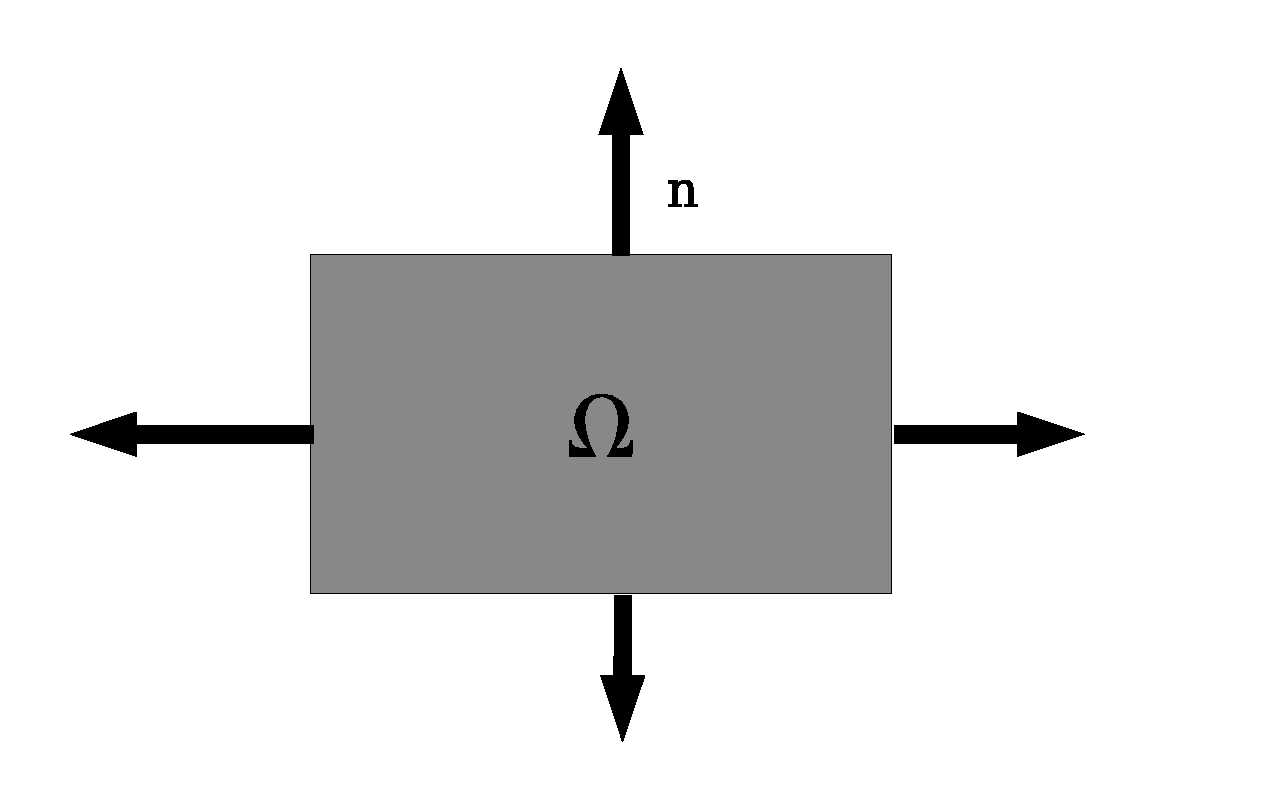
\includegraphics{FirstStepDomain}}
    \caption{Domain $\Omega=[0,1]^2$ with outer normal field $n$.}
    \label{fig:FirstSteps.1}
\end{figure}

$\Delta$ denotes the Laplace operator\index{Laplace operator}, which is defined by
\begin{equation}
\Delta u = (u_{,0})_{,0}+(u_{,1})_{,1}
\label{eq:FirstSteps.1.1}
\end{equation}
where, for any function $u$ and any direction $i$, $u_{,i}$
denotes the partial derivative \index{partial derivative} of $u$ with respect
to $i$.\footnote{You may be more familiar with the Laplace
operator\index{Laplace operator} being written as $\nabla^2$, and written in
the form
\begin{equation*}
    \nabla^2 u = \nabla^t \cdot \nabla u =  \frac{\partial^2 u}{\partial x_0^2} 
    + \frac{\partial^2 u}{\partial  x_1^2}
\end{equation*}
and \eqn{eq:FirstSteps.1} as
\begin{equation*}
    -\nabla^2 u = f
\end{equation*}
}
Basically, in the subindex of a function, any index to the right of the comma denotes a spatial derivative with respect 
to the index. To get a more compact form we will write $u_{,ij}=(u_{,i})_{,j}$
which leads to
\begin{equation}
\Delta u = u_{,00}+u_{,11}=\sum_{i=0}^2 u_{,ii}
\label{eq:FirstSteps.1.1b}
\end{equation}
We often find that use
of nested $\sum$ symbols makes formulas cumbersome, and we use the more
compact Einstein summation convention\index{summation convention}. This 
drops the $\sum$ sign and assumes that a summation is performed over any repeated index.
For instance, 
\begin{eqnarray}
x_{i}y_{i}=\sum_{i=0}^2 x_{i}y_{i}   \\
x_{i}u_{,i}=\sum_{i=0}^2 x_{i}u_{,i}   \\
u_{,ii}=\sum_{i=0}^2 u_{,ii} \\
x_{ij}u_{i,j}=\sum_{j=0}^2\sum_{i=0}^2 x_{ij}u_{i,j}   \\
\label{eq:FirstSteps.1.1c}
\end{eqnarray}
With the summation convention we can write the Poisson equation \index{Poisson equation} as
\begin{equation}
- u_{,ii} =1 
\label{eq:FirstSteps.1.sum}
\end{equation}
where $f=1$ in this example.

On the boundary of the domain $\Omega$ the normal derivative $n_{i} u_{,i}$
of the solution $u$ shall be zero, i.e. $u$ shall fulfill
the homogeneous Neumann boundary condition\index{Neumann
boundary condition!homogeneous}
\begin{equation}
n_{i} u_{,i}= 0 \;.
\label{eq:FirstSteps.2}
\end{equation}
$n=(n_{i})$ denotes the outer normal field
of the domain, see \fig{fig:FirstSteps.1}. Remember that we 
apply the Einstein summation convention \index{summation convention}, i.e. $n_{i} u_{,i}= n_{0} u_{,0} +%
n_{1} u_{,1}$.\footnote{Some readers may be more familiar with the
notation $\frac{\partial u}{\partial n} = n_{i} u_{,i}=\mathbf{n}\cdot \nabla u$.}
The Neumann boundary condition of \eqn{eq:FirstSteps.2} should be fulfilled on the
set $\Gamma^N$, the top and right edge of the domain:
\begin{equation}
    \Gamma^N=\{(x_0;x_1) \in \Omega | x_{0}=1 \mbox{ or } x_{1}=1  \}
    \label{eq:FirstSteps.2b}
\end{equation}
On the bottom and the left edge of the domain, defined
as 
\begin{equation}
    \Gamma^D=\{(x_0;x_1) \in \Omega | x_{0}=0 \mbox{ or } x_{1}=0  \}
    \label{eq:FirstSteps.2c}
\end{equation}
the solution shall be identical to zero:
\begin{equation}
    u=0 \; .
    \label{eq:FirstSteps.2d}
\end{equation}
A homogeneous Dirichlet boundary
condition\index{Dirichlet boundary condition!homogeneous}.
The partial differential equation in \eqn{eq:FirstSteps.1.sum} together
with Neumann  \eqn{eq:FirstSteps.2} and 
Dirichlet boundary conditions in \eqn{eq:FirstSteps.2d} form a so-called
boundary value
problem\index{boundary value problem} (BVP\index{boundary value problem!BVP})
for the unknown function~$u$. 

\begin{figure}[ht]
    \centerline{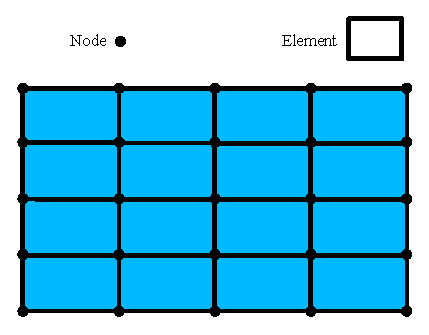
\includegraphics{FirstStepMesh}}
    \caption{Mesh of $4 \times 4$ elements on a rectangular domain. Here
    each element is a quadrilateral and described by four nodes, namely
    the corner points. The solution is interpolated by a bi-linear
    polynomial.}
    \label{fig:FirstSteps.2}
\end{figure}

In general the BVP\index{boundary value problem!BVP} cannot be solved
analytically and numerical methods are used to construct an
approximation of the solution $u$.
Here we will use the finite element method\index{finite element method}
(FEM\index{finite element method!FEM}).
The basic idea is to fill the domain with a set of points called nodes.
The solution is approximated by its values on the nodes\index{finite element method!nodes}.
Moreover, the domain is subdivided into smaller sub-domains called
elements\index{finite element method!element}.
On each element the solution is represented by a polynomial of a certain
degree through its values at the nodes located in the element.
The nodes and their connection through elements is called a
mesh\index{finite element method!mesh}. \fig{fig:FirstSteps.2} shows an
example of a FEM mesh with four elements in the $x_0$ and four elements
in the $x_1$ direction over the unit square.
For more details we refer the reader to the literature, for instance \Refe{Zienc,NumHand}.

The \escript solver we want to use to solve this problem is embedded into the \PYTHON interpreter language.
So you can solve the problem interactively but you will learn quickly that it
is more efficient to use scripts which can be edited with your favorite editor.
To enter the escript environment, use the \program{run-escript}
command\footnote{\program{run-escript} is not available under Windows.
If you run under Windows you can just use the \program{python} command and the
\env{OMP_NUM_THREADS} environment variable to control the number of threads.}:
\begin{verbatim}
run-escript
\end{verbatim}
which will pass you on to the \PYTHON prompt
\begin{verbatim}
Python 2.7.6 (default, Mar 22 2014, 15:40:47) 
[GCC 4.8.2] on linux2
Type "help", "copyright", "credits" or "license" for more information.
>>> 
\end{verbatim}
Here you can use all available \PYTHON commands and language features\footnote{Throughout our examples, we use the python 3 form of 
print. That is, print(1) instead of print 1.}, for instance
\begin{python}
  >>> x=2+3
  >>> print("2+3=",x)
  2+3= 5
\end{python}
We refer to the \PYTHON user's guide if you are not familiar with \PYTHON.

\escript provides the class \Poisson to define a Poisson equation\index{Poisson equation}.
(We will discuss a more general form of a PDE\index{partial differential equation!PDE} 
that can be defined through the \LinearPDE class later.)
The instantiation of a \Poisson class object requires the specification of the domain $\Omega$.
In \escript \Domain class objects are used to describe the geometry of a
domain but it also contains information about the discretization methods and
the solver used to solve the PDE.
Here we use the FEM\index{finite element method} library \finley.
The following statements create the \Domain object \var{mydomain} from the 
\finley function \method{Rectangle}:
\begin{python}
  from esys.finley import Rectangle
  mydomain = Rectangle(l0=1.,l1=1.,n0=40, n1=20)
\end{python}
In this case the domain is a rectangle with the lower left corner at point $(0,0)$
and the upper right corner at $(\var{l0},\var{l1})=(1,1)$.
The arguments \var{n0} and \var{n1} define the number of elements in $x_{0}$ and
$x_{1}$-direction respectively. For more details on \method{Rectangle} and
other \Domain generators see \Chap{chap:finley}, \Chap{chap:ripley}, and
\Chap{chap:speckley}.

The following statements define the \Poisson class object \var{mypde} with domain \var{mydomain} and
the right hand side $f$ of the PDE to constant $1$: 
\begin{python}
  from esys.escript.linearPDEs import Poisson
  mypde = Poisson(mydomain)
  mypde.setValue(f=1)
\end{python}
We have not specified any boundary condition but the \Poisson class implicitly
assumes homogeneous Neuman boundary conditions\index{Neumann boundary condition!homogeneous} defined by \eqn{eq:FirstSteps.2}.
With this boundary condition the BVP\index{boundary value problem!BVP} we have
defined has no unique solution.
In fact, with any solution $u$ and any constant $C$ the function $u+C$ becomes
a solution as well.
We have to add a Dirichlet boundary condition\index{Dirichlet boundary condition}.
This is done by defining a characteristic function\index{characteristic function}
which has positive values at locations $x=(x_{0},x_{1})$
where Dirichlet boundary condition is set and $0$ elsewhere.
In our case of $\Gamma^D$ defined by \eqn{eq:FirstSteps.2c}, we need to
construct a function \var{gammaD} which is positive for the cases $x_{0}=0$ or $x_{1}=0$.
To get an object \var{x} which contains the coordinates of the nodes in the domain use
\begin{python}
  x=mydomain.getX() 
\end{python}
The method \method{getX} of the \Domain \var{mydomain} gives access to locations
in the domain defined by \var{mydomain}.
The object \var{x} is actually a \Data object which will be discussed in
\Chap{ESCRIPT CHAP} in more detail.
What we need to know here is that \var{x} has \Rank (number of dimensions) and
a \Shape (list of dimensions) which can be viewed by calling the \method{getRank} and \method{getShape} methods:
\begin{python}
  print("rank ",x.getRank(),", shape ",x.getShape())
\end{python}
This will print something like
\begin{python}
  rank 1, shape (2,)
\end{python}
The \Data object also maintains type information which is represented by the 
\FunctionSpace of the object. For instance
\begin{python}
  print(x.getFunctionSpace())
\end{python}
will print 
\begin{python}
  Finley_Nodes [ContinuousFunction(domain)] on FinleyMesh 
\end{python}
which tells us that the coordinates are stored on the nodes of (rather than on
points in the interior of) a Finley mesh.
To get the  $x_{0}$ coordinates of the locations we use the statement 
\begin{python}
  x0=x[0]
\end{python}
Object \var{x0} is again a \Data object now with \Rank $0$ and \Shape $()$.
It inherits the \FunctionSpace from \var{x}:
\begin{python}
  print(x0.getRank(), x0.getShape(), x0.getFunctionSpace())
\end{python}
will print
\begin{python}
  0 () Finley_Nodes [ContinuousFunction(domain)] on FinleyMesh
\end{python}
We can now construct a function \var{gammaD} which is only non-zero on the
bottom and left edges of the domain with
\begin{python}
  from esys.escript import whereZero
  gammaD=whereZero(x[0])+whereZero(x[1])
\end{python}

\code{whereZero(x[0])} creates a function which equals $1$ where \code{x[0]} is (almost) equal to zero and $0$ elsewhere. 
Similarly, \code{whereZero(x[1])} creates a function which equals $1$ where \code{x[1]} is equal to zero and $0$ elsewhere.
The sum of the results of \code{whereZero(x[0])} and \code{whereZero(x[1])}
gives a function on the domain \var{mydomain} which is strictly positive where $x_{0}$ or $x_{1}$ is equal to zero.
Note that \var{gammaD} has the same \Rank, \Shape and \FunctionSpace as \var{x0} used to define it.
So from 
\begin{python}
  print(gammaD.getRank(), gammaD.getShape(), gammaD.getFunctionSpace())
\end{python}
one gets 
\begin{python}
  0 () Finley_Nodes [ContinuousFunction(domain)] on FinleyMesh
\end{python}
An additional parameter \var{q} of the \code{setValue} method of the \Poisson
class defines the characteristic function\index{characteristic function} of
the locations of the domain where the homogeneous Dirichlet boundary condition\index{Dirichlet boundary condition!homogeneous} is set.
The complete definition of our example is now:
\begin{python}
  from esys.escript.linearPDEs import Poisson
  x = mydomain.getX()
  gammaD = whereZero(x[0])+whereZero(x[1])
  mypde = Poisson(domain=mydomain)
  mypde.setValue(f=1,q=gammaD)
\end{python}
The first statement imports the \Poisson class definition from the \linearPDEs module.
To get the solution of the Poisson equation defined by \var{mypde} we just have to call its \method{getSolution} method. 

Now we can write the script to solve our Poisson problem
\begin{python}
  from esys.escript import *
  from esys.escript.linearPDEs import Poisson
  from esys.finley import Rectangle
  # generate domain:
  mydomain = Rectangle(l0=1.,l1=1.,n0=40, n1=20)
  # define characteristic function of Gamma^D
  x = mydomain.getX()
  gammaD = whereZero(x[0])+whereZero(x[1])
  # define PDE and get its solution u
  mypde = Poisson(domain=mydomain)
  mypde.setValue(f=1, q=gammaD)
  u = mypde.getSolution()
\end{python}
The question is what we do with the calculated solution \var{u}.
Besides postprocessing, e.g. calculating the gradient or the average value,
which will be discussed later, plotting the solution is one of the things you
might want to do.
\escript offers two ways to do this, both based on external modules or packages.
The first option uses the \MATPLOTLIB module which allows plotting of 2D
results relatively quickly from within the \PYTHON script, see~\cite{matplotlib}.
However, there are limitations when using this tool, especially for large
problems and when solving three-dimensional problems.
Therefore, \escript provides functionality to export data as files which can
subsequently be read by third-party software packages such as
\mayavi\cite{mayavi} or \VisIt~\cite{VisIt}.

\subsection{Plotting Using \MATPLOTLIB}
The \MATPLOTLIB module provides a simple and easy-to-use way to visualize PDE
solutions (or other \Data objects).
To hand over data from \escript to \MATPLOTLIB the values need to be mapped onto
a rectangular grid. We will make use of the \numpy module for this.

First we need to create a rectangular grid which is accomplished by the following statements:
\begin{python}
  import numpy
  x_grid = numpy.linspace(0., 1., 50)
  y_grid = numpy.linspace(0., 1., 50)
\end{python}
\var{x_grid} is an array defining the x coordinates of the grid while
\var{y_grid} defines the y coordinates of the grid.
In this case we use $50$ points over the interval $[0,1]$ in both directions. 

Now the values created by \escript need to be interpolated to this grid.
We will use the \SCIPY \function{interpolate.griddata} function to do this.
Spatial coordinates are easily extracted as a \var{list} by
\begin{python}
  x=mydomain.getX()[0].toListOfTuples()
  y=mydomain.getX()[1].toListOfTuples()
\end{python}
In principle we can apply the same \member{toListOfTuples} method to extract the values from the PDE solution \var{u}.
However, we have to make sure that the \Data object we extract the values from
uses the same \FunctionSpace as we have used when extracting \var{x} and \var{y}.
We apply the \function{interpolation} to \var{u} before extraction to achieve this:
\begin{python}
  z=interpolate(u, mydomain.getX().getFunctionSpace())
\end{python}
The values in \var{z} are the values at the points with the coordinates given by \var{x} and \var{y}.
These values are interpolated to the grid defined by \var{x_grid} and \var{y_grid} by using
\begin{python}
   import scipy.interpolate
   z_grid = scipy.interpolate.griddata((x,y),z,(x_grid[None,:],y_grid[:,None]),'linear')
\end{python}
Now \var{z_grid} gives the values of the PDE solution \var{u} at the grid which can be plotted using \function{contourf}:
\begin{python}
  import matplotlib
  matplotlib.pyplot.contourf(x_grid, y_grid, z_grid, 5)
  matplotlib.pyplot.savefig("u.png")
\end{python}
Here we use 5 contours. The last statement writes the plot to the file \file{u.png} in the PNG format.
Alternatively, one can use 
\begin{python}
  matplotlib.pyplot.contourf(x_grid, y_grid, z_grid, 5)
  matplotlib.pyplot.show()
\end{python}
which gives an interactive browser window.

\begin{figure}
\centerline{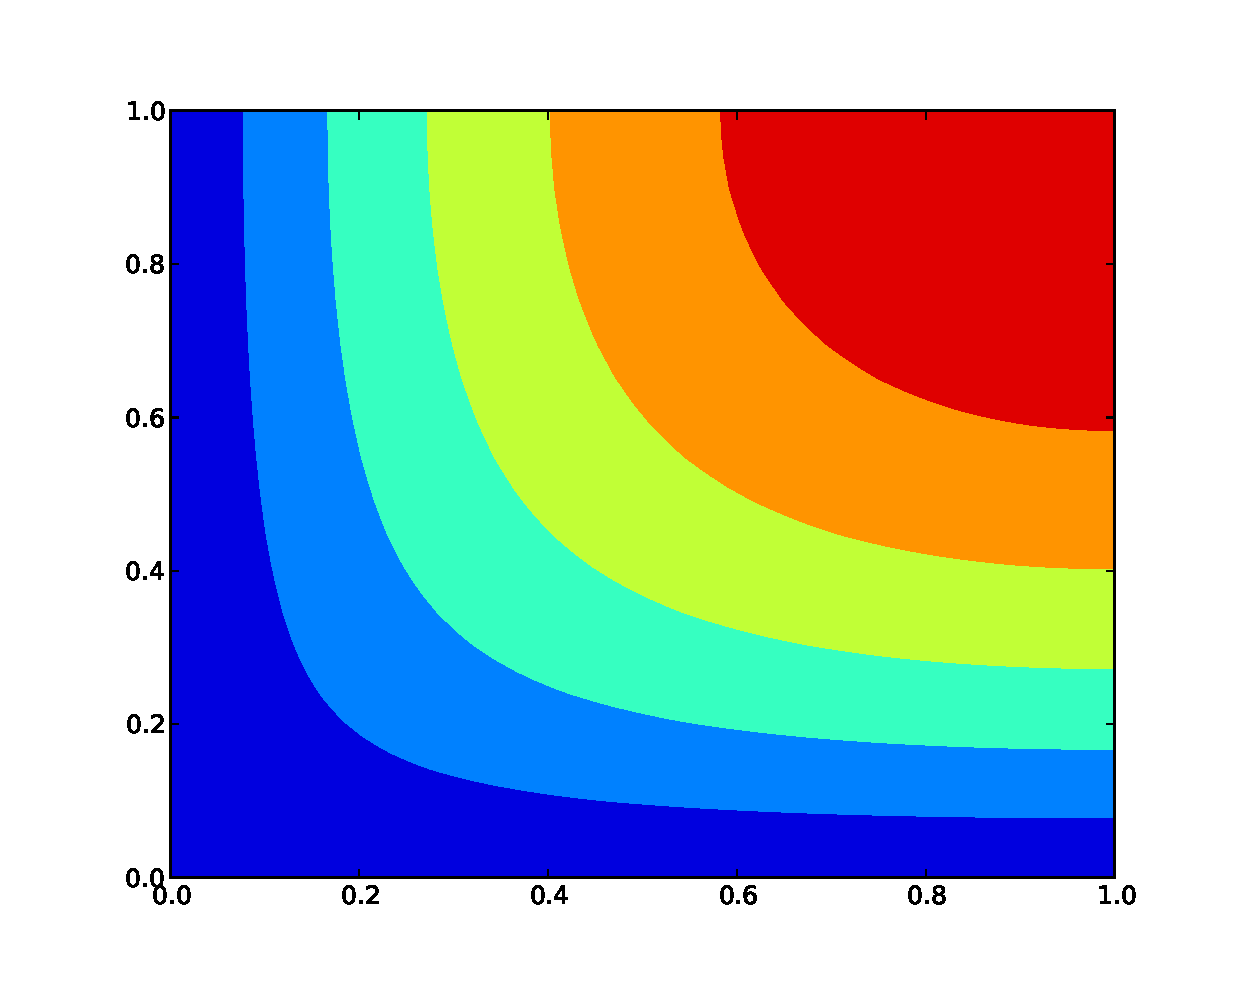
\includegraphics[width=\figwidth]{FirstStepResultMATPLOTLIB}}
\caption{Visualization of the Poisson Equation Solution for $f=1$ using \MATPLOTLIB}
\label{fig:FirstSteps.3b}
\end{figure}

Now we can write the script to solve our Poisson problem
\begin{python}
  from esys.escript import *
  from esys.escript.linearPDEs import Poisson
  from esys.finley import Rectangle
  import scipy.interpolate
  import numpy
  import matplotlib

  import pylab
  # generate domain:
  mydomain = Rectangle(l0=1.,l1=1.,n0=40, n1=20)
  # define characteristic function of Gamma^D
  x = mydomain.getX()
  gammaD = whereZero(x[0])+whereZero(x[1])
  # define PDE and get its solution u
  mypde = Poisson(domain=mydomain)
  mypde.setValue(f=1,q=gammaD)
  u = mypde.getSolution()
  # interpolate u to a matplotlib grid:
  x_grid = numpy.linspace(0.,1.,50)
  y_grid = numpy.linspace(0.,1.,50)
  x=mydomain.getX()[0].toListOfTuples()
  y=mydomain.getX()[1].toListOfTuples()
  z=interpolate(u,mydomain.getX().getFunctionSpace()).toListOfTuples()
  z_grid = scipy.interpolate.griddata((x,y),z,(x_grid[None,:],y_grid[:,None]),'linear')
  # interpolate u to a rectangular grid:
  matplotlib.pyplot.contourf(x_grid, y_grid, z_grid, 5)
  matplotlib.pyplot.savefig("u.png")
\end{python}
The entire code is available as \file{poisson_matplotlib.py} in the \ExampleDirectory.
You can run the script using the {\it escript} environment
\begin{verbatim}
run-escript poisson_matplotlib.py
\end{verbatim}
This will create a file called \file{u.png}, see \fig{fig:FirstSteps.3b}.
For details on the usage of the \MATPLOTLIB module we refer to the documentation~\cite{matplotlib}.

As pointed out, \MATPLOTLIB is restricted to the two-dimensional case and
should be used for small problems only.
It can not be used under \MPI as the \member{toListOfTuples} method is not
safe under \MPI\footnote{The phrase 'safe under \MPI' means that a program
will produce correct results when run on more than one processor under \MPI.}.

\begin{figure}
\centerline{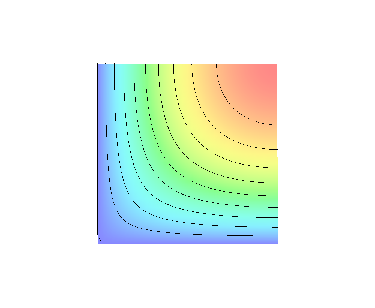
\includegraphics[width=\figwidth]{FirstStepResult}}
\caption{Visualization of the Poisson Equation Solution for $f=1$}
\label{fig:FirstSteps.3}
\end{figure}

\subsection{Visualization using export files}

As an alternative to \MATPLOTLIB, {\it escript} supports exporting data to
\VTK and \SILO files which can be read by visualization tools such as
\mayavi\cite{mayavi} and \VisIt~\cite{VisIt}. This method is \MPI safe and
works with large 2D and 3D problems.

To write the solution \var{u} of the Poisson problem in the \VTK file format
to the file \file{u.vtu} one needs to add:
\begin{python}
  from esys.weipa import saveVTK
  saveVTK("u.vtu", sol=u)
\end{python}
This file can then be opened in a \VTK compatible visualization tool where the
solution is accessible by the name {\it sol}. Similarly,
\begin{python}
  from esys.weipa import saveSilo
  saveSilo("u.silo", sol=u)
\end{python}
will write \var{u} to a \SILO file if escript was compiled with support for
LLNL's \SILO library.

The Poisson problem script is now 
\begin{python}
  from esys.escript import *
  from esys.escript.linearPDEs import Poisson
  from esys.finley import Rectangle
  from esys.weipa import saveVTK
  # generate domain:
  mydomain = Rectangle(l0=1.,l1=1.,n0=40, n1=20)
  # define characteristic function of Gamma^D
  x = mydomain.getX()
  gammaD = whereZero(x[0])+whereZero(x[1])
  # define PDE and get its solution u
  mypde = Poisson(domain=mydomain)
  mypde.setValue(f=1,q=gammaD)
  u = mypde.getSolution()
  # write u to an external file
  saveVTK("u.vtu",sol=u)
\end{python}
The entire code is available as \file{poisson_vtk.py} in the \ExampleDirectory.

You can run the script using the {\it escript} environment and visualize the
solution using \mayavi:
\begin{verbatim}
run-escript poisson_vtk.py
mayavi2 -d u.vtu -m Surface
\end{verbatim}
The result is shown in \fig{fig:FirstSteps.3}.


% $Id$
\chapter{How to Solve The Diffusion Equation}
\label{DIFFUSION CHAP}

\begin{figure}
\centerline{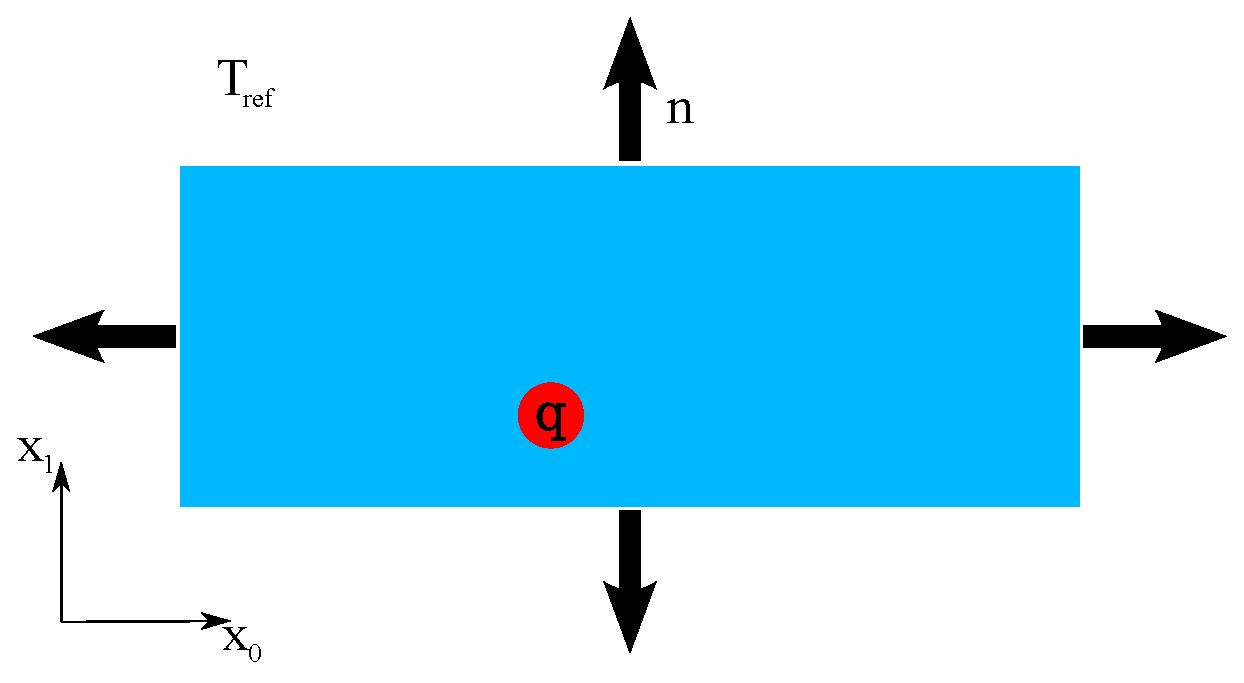
\includegraphics[width=\figwidth]{DiffusionDomain}}
\caption{Temperature Diffusion Problem with Circular Heat Source}
\label{DIFFUSION FIG 1}
\end{figure}

\begin{figure}
\centerline{
\includegraphics[width=\figwidth]{DiffusionRes1}}
\centerline{
\includegraphics[width=\figwidth]{DiffusionRes16}}
\centerline{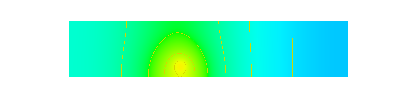
\includegraphics[width=\figwidth]{DiffusionRes32}}
\centerline{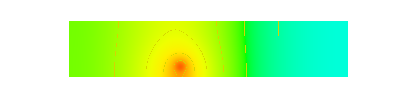
\includegraphics[width=\figwidth]{DiffusionRes48}}
\caption{Results of the Temperture Diffusion Problem for Time Steps $1$ $16$, $32$ and $48$.}
\label{DIFFUSION FIG 2}
\end{figure}


\section{\label{DIFFUSION OUT SEC}Outline}
In this chapter we will discuss how to solve the time depeneded-temperature diffusion\index{diffusion equation} within
a block of material. Within the block there is a heat source which drives the temperature diffusion.
On the surface energy can radiate into the surrounding environment.
\fig{DIFFUSION FIG 1} shows the configuration.

In the next \Sec{DIFFUSION TEMP SEC} we will present the relevant model. A 
time integration scheme is introduced to calculate the temperature at given time nodes $t^{(n)}$. 
We will see that at time step a so-called Helmholtz equation \index{Helmholtz equation} has to be solved. 
The implementation iof a Helmholtz equation solver will be discussed in \Sec{DIFFUSION HELM SEC}. 
In Section~\ref{DIFFUSION TRANS SEC} the solver of the Helmholtz equation is used to build a
solver for the temperature diffusion problem. 

\section{\label{DIFFUSION TEMP SEC}Temperature Diffusion}

The temperature $T$ is a function of its location in the domain and time $t>0$. The governing equation
in the interior of the domain is given by
\begin{equation}
\rho c\hackscore p T\hackscore{,t} - (\kappa T\hackscore{,i})\hackscore{,i} = q
\label{DIFFUSION TEMP EQ 1}
\end{equation}
where $\rho c\hackscore p$ and $\kappa$ are given material constants. In case of a composite
material the parameters are depending on the their location in the domain. $q$ is
a heat source (or sink) within the domain. We are using Einstein summation convention \index{summation convention} 
as introduced in \Chap{FirstSteps}. In our case we assume $q$ to be equal to a constant $q^{c}$
on a circle or sphere with center $x^c$ and radius $r$ and $0$ elsewhere:
\begin{equation}
q(x,t)=
\left\{ 
\begin{array}{lcl}
q^c  & & \|x-x^c\| \le r \\
     & \mbox{if} \\
0    &  & \mbox{else} \\
\end{array}
\right.
\label{DIFFUSION TEMP EQ 1b}
\end{equation}
for all $x$ in the domain and all time  $t>0$.

On the surface of the domain we are 
are specifying a radiation condition 
which precribes the normal component of the flux $J\hackscore i= \kappa T\hackscore{,i}$ to be proportional
to the difference of the current temperature to the surrounding temperature $T\hackscore{ref}$:    
\begin{equation}
 \kappa T\hackscore{,i} n\hackscore i = \eta (T\hackscore{ref}-T) 
\label{DIFFUSION TEMP EQ 2}
\end{equation}
$\eta$ is a given material coefficient depending on the material and the surrounding medium. 
As usual $n_i$ is the $i$-th component of the outer normal field \index{outer normal field}
at the surface of the domain. 

To solve the the time depended \eqn{DIFFUSION TEMP EQ 1} the initial temperature at time 
$t=0$ has to be given. Here we assume that the initial temperature is the surrounding temperature:
\begin{equation}
T(x,0)=T\hackscore{ref} 
\label{DIFFUSION TEMP EQ 4}
\end{equation}
for all $x$ in the domain. It is pointed out that 
the initial conditions is fullfilling the 
boundary condition defined by \eqn{DIFFUSION TEMP EQ 2}. 

The temperature is calculated discrete time nodes $t^{(n)}$ where 
$t^{(0)}=0$ and  $t^{(n)}=t^{(n-1)}+h$ where $h>0$ is the step size which is assumed to be constant. 
In the following the upper index ${(n)}$ is refering to a value at time $t^{(n)}$. The simplest
and most robust scheme to approximate the time derivative of the the temperature is the 
\index{backward Euler} scheme, see~\cite{XXX} for alternatives. The backward Euler scheme bases
on the Taylor expansion
\begin{equation}
T^{(n-1)}\approx T^{(n)}+T\hackscore{,t}^{(n)}(t^{(n-1)}-t^{(n)})
=T^{(n-1)} + h \cdot T\hackscore{,t}^{(n)}
\label{DIFFUSION TEMP EQ 6}
\end{equation}
which is inserted into \eqn{DIFFUSION TEMP EQ 1}. By separating the terms at 
$t^{(n)}$ and  $t^{(n-1)}$ one gets for $n=1,2,3\ldots$
\begin{equation}
\frac{\rho c\hackscore p}{h} T^{(n)} - (\kappa T^{(n)}\hackscore{,i})\hackscore{,i} = q +  \frac{\rho c\hackscore p}{h} T^{(n-1)}
\label{DIFFUSION TEMP EQ 7}
\end{equation}
where $T^{(0)}=T\hackscore{ref}$ is taken form the initial condition given by \eqn{DIFFUSION TEMP EQ 4}.
Together with the natural boundary condition from \eqn{DIFFUSION TEMP EQ 2}.
this forms a boundary value problem that has to be solved for each time step. 
As a first step to implement a solver for the temperature diffusion problem we will 
first implement a solver for the  boundary value problem that has to be solved at each time step.

\section{\label{DIFFUSION HELM SEC}Helmholtz Problem}
The partial differential equation to be solved for $T^{(n)}$ has the form 
\begin{equation}
\omega u  - (\kappa u\hackscore{,i})\hackscore{,i} = f
\label{DIFFUSION HELM EQ 1}
\end{equation}
where $u$ plays the role of $T^{(n)}$ and we set
\begin{equation}
\omega=\frac{\rho c\hackscore p}{h} \mbox{ and } f=q+\frac{\rho c\hackscore p}{h}T^{(n-1)} \;.
\label{DIFFUSION HELM EQ 1b}
\end{equation}
With $g=\eta T\hackscore{ref}$ the radiation condition defined by \eqn{DIFFUSION TEMP EQ 2}
takes the form 
\begin{equation}
\kappa u\hackscore{,i} n\hackscore{i} =  g - \eta u\mbox{ on } \Gamma
\label{DIFFUSION HELM EQ 2}
\end{equation}
The partial differential 
\eqn{DIFFUSION HELM EQ 1} together with boundary conditions of \eqn{DIFFUSION HELM EQ 2}
is called a Helmholtz equation \index{Helmholtz equation}. 

We want to use the \LinearPDE class provided by \escript to define and solve a general linear PDE such as the 
Helmholtz equation. We have used a special case of the \LinearPDE class, namely the
\Poisson class already in \Chap{FirstSteps}. 
Here we will write our own specialized class of the \LinearPDE to solve the Helmholtz equation. 

The general form of a single PDE that can be handeled by the \LinearPDE class is 
\begin{equation}\label{EQU.FEM.1}
-(A\hackscore{jl} u\hackscore{,l})\hackscore{,j}+D u =Y \; .
\end{equation}
The general form and systems is discussed in \Sec{SEC LinearPDE}.  
$A$, $D$ and $Y$ are the known coeffecients of the PDE \index{partial differential equation!coefficients}. 
Notice that $A$ is a matrix or tensor of order 2 and $D$ and $Y$ are scalar. 
They may be constant or may depend on their 
location in the domain but must not depend on the unknown solution $u$. 
The following natural boundary conditions \index{boundary condition!natural} that
are used in the \LinearPDE class have the form
\begin{equation}\label{EQU.FEM.2}
n\hackscore{j}A\hackscore{jl} u\hackscore{,l}+du=y  \;.
\end{equation}
where, as usual, $n$ denotes the outer normal field on the surface of the domain. Notice that 
the coefficient $A$ is already used in the PDE in \eqn{EQU.FEM.1}. $d$ and $y$ are given scalar coefficients.

By inpecting the Helmholtz equation \index{Helmholtz equation} 
we can easily assign values to the coefficients in the 
general PDE of the \LinearPDE class:
\begin{equation}\label{DIFFUSION HELM EQ 3}
\begin{array}{llllll}
A\hackscore{ij}=\kappa \delta\hackscore{ij} & D=\omega & Y=f \\
d=\eta & y= g &  \\
\end{array}
\end{equation}
$\delta\hackscore{ij}$ is the Kronecker symbol \index{Kronecker symbol} defined by $\delta=\hackscore{ij}=1$ for
$i=j$ and $0$ otherwise.

We want to implement a 
new class which we will call \class{Helmholtz} that provides the same methods like the \LinearPDE class but
is defined through the coefficeints $\kappa$, $\omega$, $f$, $\eta$, 
$g$ rather than the general form given by \eqn{EQU.FEM.1}.
Python's
mechanism of inhertence allows doing this in a very easy way. 
The advantage is that our new \class{Helmholtz} can be used in any context 
that works with a \LinearPDE class but with an easier interface to define the PDE.
This improves reuasablity as well as maintainability of program codes.

We want to implement a 
new class which we will call \class{Helmholtz} that provides the same methods like the \LinearPDE class but
is defined through the coefficeints $\kappa$, $\omega$, $f$, $\alpha$, 
$g$ rather than the general form given by \eqn{EQU.FEM.1}. 
Python's mechanism of subclasses allows doing this in a very easy way.
The \Poisson class of the \linearPDEsPack module,
which we have already used in \Chap{FirstSteps}, is in fact a subclass of the 
\LinearPDE class. That means that it all methods (such as the \method{getSolution})
from the parent class \LinearPDE are defined for any \Poisson object. However, new
methods can be added and methods of the parent class can be redefined. In fact,
the \Poisson class redefines the \method{setValue} of the \LinearPDE class which is called to assign 
values to the coefficients of the PDE. This is exactly what we will do when we define 
our new \class{Helmholtz} class:
\begin{python}
from esys.linearPDEs import LinearPDE
import numarray
class Helmholtz(LinearPDE)
   def setValue(self,kappa=0,omega=1,f=0,eta=0,g=0)
        self._setValue(A=kappa*numarray.identity(self.getDim()),D=omega,Y=f,d=eta,y=g)
\end{python}
\code{class Helmholtz(linearPDE)} declares the new \class{Helmholtz} class as a subclass 
of the \LinearPDE which have imported in the first line of the script. 
We add the method \method{setValue} to the class which overwrites the 
\method{setValue} method of the \LinearPDE class. The new methods which has the 
parameters of the Helmholtz \eqn{DIFFUSION HELM EQ 1} as arguments 
maps the parameters of the coefficients of the general PDE defined 
in \eqn{EQU.FEM.1}. The coefficient \var{A} is defined by Kroneckers symbol. we use the
\numarray function \function{identity} which return a square matrix which has ones on the
main diagonal and zeros out side the main diagonal. The argument of \function{identity} gives the order of the matrix.
Here we use
the \method{getDim} of the \LinearPDE class object \var{self} to get the spatial dimension of the domain of the
PDE. As we will make use of the \class{Helmholtz} class several times, it is convient to 
put is definition into a file which we name \file{mytools.py} available in the \ExampleDirectory.
You can use your favourite editor to create and edit the file.   

An object of the \class{Helmholtz} class is created through the statments:
\begin{python}
from mytools import *
mypde=Helmholtz(mydomain)
mypde.setValue(kappa=10.,omega=0.1,f=12)
u=mypde.getSolution()
\end{python}
In the first statement we import all definition from the \file{mytools.py}  \index{scripts!\file{mytools.py}}. Make sure
that \file{mytools.py} is in directory from where you have started Python.
\var{mydomain} is the \Domain of the PDE. In the third statment values are
assigned to the PDE parameters. As no values for arguments \var{eta} and \var{g} are
specified the default values $0$ are used \footnote{It would be better to use the default value 
\var{escript.Data()} rather then $0$ as then the coefficient would be defined as being not present and
would not be processed when the PDE is evaluated.}. In the forth statement the solution of the
PDE is returned. 

We want to test our \class{Helmholtz} class on a rectangular domain
of length $l$ and height $h$. We do this by choosing a simple test solution,
here we take $u=x\hackscore{0}$ and then calculate the right hand side terms $f$ and $g$ such that
the test solution becomes the solution of the problem. If we take $\kappa=1$ 
an easy calculation shows that we have to choose $f=\omega \cdot x\hackscore{0}$. On the boundary we get
$\kappa n\hackscore{i} u\hackscore{,i}=n\hackscore{0}$.  
So we have to set $g=n\hackscore{0}+\eta x\hackscore{0}$. The following script \file{helmholtztest.py} 
\index{scripts!\file{helmholtztest.py}} which is available in the \ExampleDirectory
implements this test problem using the \finley PDE solver:
\begin{python}
from mytools import *
from esys.escript import *
import esys.finley
#... set some parameters ...
omega=0.1
eta=10.
#... generate domain ...
mydomain = esys.finley.Rectangle(l0=5.,l1=1.,n0=50, n1=10)
#... open PDE and set coefficients ...
mypde=Helmholtz(mydomain)
n=mydomain.getNormal()
x=mydomain.getX()
mypde.setValue(1,omega,omega*x[0],eta,n[0]+eta*x[0])
#... calculate error of the PDE solution ...
u=mypde.getSolution()
print "error is ",Lsup(u-x[0])
\end{python}
The script is similar to the script \file{mypoisson.py} dicussed in \Chap{FirstSteps}.
\code{mydomain.getNormal()} returns the outer normal field on the surface of the domain. The function \function{Lsup}
is imported by the \code{from escript import *} statement and returns the maximum absulute value of it argument. To run 
The error shown by the print statement should be in the order of $10^{-7}$. As piecewise linear interpolation is
used to approximate the solution and our solution is a linear function of the spatial coordinates one may 
expect that the error is zero. However, as most PDE packages uses an iterative solver which is terminated
when a given tolerance has been reached. The default tolerance is $10^{-8}$. Thsi value can be altered by using the 
\method{setTolerance} of the \LinearPDE class. 

\section{The Transition Problem}
\label{DIFFUSION TRANS SEC}
Now we are ready to solve the original time dependent problem. The main 
part of the script is the loop over the time $t$ which takes the following form:
\begin{python}
mypde=Helmholtz(mydomain)
while t<t_end:
      mypde.setValue(kappa,rhocp/h,q+rhocp/h*T,eta,eta*Tref)
      T=mypde.getSolution()
      t+=h
\end{python}
\var{kappa}, \var{rhocp}, \var{eta} and \var{Tref} are input parameters of the model. \var{q} is the heat source
in the domain and \var{h} is the time step size which has to be chosen. Notice that the \class{Hemholtz}
is created before the loop over time is entered while in each time step only the coefficients
are reset in each time step. This way some information about the reperesentation of the PDE can be reused 
\footnote{The efficience can be improved further by setting the coefficients in the operator
\var{kappa}, \var{omega} and \var{eta} before entering the \code{while}-loop and only update the coefficients
in the right hand side \var{f} and \var{g}. This needs a more careful implementation of the \method{setValue}
method but gives the advantage that the \LinearPDE class can save rebuilding the PDE operator}. The variable \var{T}
holds the current temperature. It is used to calculate the right hand side coefficient \var{f} in the
Helmholtz \eqn{DIFFUSION HELM EQ 1}. Statement \code{T=mypde.getSolution()} overwrites \var{T} with the 
temperature of the new time step $\var{t}+\var{h}$. To get this iterative process going we need to sepcify the
initial temperature distribution, which equal to $T\hackscore{ref}$.

The heat source \var{q} which is defined in \eqn{DIFFUSION TEMP EQ 1b} shall be \var{q0}
at an area defined as a circle of radius \var{r} and center \var{xc} and zero outside this circle.
\var{q0} is a fixed constant. The following script defines \var{q} as desired:  
\begin{python}
xc=[0.02,0.002]
r=0.001
x=mydomain.getX()
q=q0*(length(x-xc)-r).whereNegative()
\end{python}
\var{x} is a \Data class object of
the \escript module defining the locations of points in the \Domain \var{mydomain}. 
\code{length(x-xc)} calculates the distances in the Euclidean norm 
of the locations \var{x} to the center of the circle \var{xc} where the heat source is acting.
Notice that the coordinates of \var{xc} are defined as a list of floating point numbers. It is independently
converted into a \Data class object before subtracted from \var{x}. The method \method{whereNegative} of
a \Data class object, in this case the result of the expression 
\code{length(x-xc)-r}, returns a \Data class which is equal one where the object negative and
zero elsewhere. After multiplication with \var{q0} we get a function with the deired property.

Now we can put the components together to the script \file{diffusion.py} which is available in the \ExampleDirectory:
\index{scripts!\file{diffusion.py}}:
\begin{python}
from mytools import *
from esys.escript import *
import esys.finley
#... set some parameters ...
x_c=[0.02,0.002]
r=0.001
q0=50.e6
Tref=0.
rhocp=2.6e6
eta=75.
kappa=240.
t_end=5.
# ...time step size and counter ...
h=0.1
i=0
t=0
#... generate domain ...
mydomain = esys.finley.Rectangle(l0=0.05,l1=0.01,n0=250, n1=50)
#... open PDE ...
mypde=Helmholtz(mydomain)
# ... set heat source: ....
x=mydomain.getX()
q=q0*(length(x-x_c)-r).whereNegative()
# ... set initial temperature ....
T=Tref
# ... start iteration:
while t<t_end:
      i+=1
      t+=h
      print "time step :",t
      mypde.setValue(kappa=kappa,omega=rhocp/h,f=q+rhocp/h*T,eta=eta,g=eta*Tref)
      T=mypde.getSolution()
      T.saveDX("T%d.dx"%i)
\end{python}
The script will create the files \file{T.1.dx},
 \file{T.2.dx}, $\ldots$, \file{T.50.dx} in the directory where the script has been started. The files give the 
temperature distributions at time steps $1$, $2$, $\ldots$, $50$ in the \OpenDX file format. 
An easy way to visualize the results is the command
\begin{verbatim}
dx -edit diffusion.net
\end{verbatim}
where \file{diffusion.net} is an \OpenDX script available in the \ExampleDirectory. 
\fig{DIFFUSION FIG 2} shows the result for some selected time steps.


% \input{wavepropagation}

% $Id$

\chapter{The module \escript}

\declaremodule{extension}{escript} \modulesynopsis{Handling data on
data points like \class{Nodes}, \class{Elements}}

The class \Data of the module \escript allows handling
data which are hold on data points \index{data points}. Examples for
data points are nodes or the quadrature points in elements of a finite
element mesh. Another examples a particles or the connection between
particles in the case of discrete element methods.  Handlers to data
points are issued by the structure which contains the data points,
e.g. a \finley mesh.

The simplest form of data attached to a data point is a single scalar
$a$ value which for instance represent the temperature or pressure at
this particular data point. Another example is a velocity field. in
this case each data point holds a vector $a(0),a(1),a(2)$ representing
the velocity at the particular data point. For the case that the
values are representing a stress tensor the value is a matrix of the
form
$a(0,0),a(0,1),a(0,2),a(1,0),a(1,1),a(1,2),a(2,0),a(2,1),a(2,2)$. In
general, values hald by data points can have up to four indices. The
number of indices is called rank \index{rank}. The tuple of length
rank which defines the upper-bound for each index component is called
the shape. A stress has rank 2 and the shape is (3,3). For a vector we
have rank 1 and shape (3,). A scalar can have rank 0 or rank 1 with
shape (1,).

In general, the data are stored for each data point. This status of
the data is called expanded \index{expanded}. But in some cases, all
data points hold the same value. In this case only a single value is
stored, which is refered by each data point if needed. This saves
memory as well as compute time. In some cases, it is very usefull to
have slightly more general way which allows to define piecewise
constant data. For this, each data point has to wear a tag which is an
integer \index{tag}. The tag is used to distingish between various
types of data points. Typical example of the usage of tags is to
assign different material parameters to various subdomains. Then one
assigns the same tag to all elements in a finite element mesh which
lay in the same subdomain.  Later each tag can be assigns individual
material parameters.

The following table shows unitary operations that can be applied to an
\Data object \var{arg}:
\begin{tableii}{l|l}{textrm}{expression}{Description}
\lineii{+\var{arg}} {just \var{arg} \index{+}}
\lineii{-\var{arg}} {swapping the sign\index{-}}
\lineii{\function{abs}(\var{arg})} {absolute value}
\lineii{\function{sin}(\var{arg})} {sine function}
\lineii{\function{cos}(\var{arg})} {cosine function}
\lineii{\function{exp}(\var{arg})} {exponential function}
\lineii{\function{sqrt}(\var{arg})} {square root}
\end{tableii}
An unitary operation returns a \Data objects of the same shape
and defined on the data points like \var{arg}.

The following table shows binary operations that can be applied to
\Data objects:
\begin{tableii}{l|l}{textrm}{expression}{Description}
\lineii{\var{arg1}+\var{arg2}} {adds \var{arg1} and \var{arg2} \index{+}}
\lineii{\var{arg1}*\var{arg2}} {multiplies \var{arg1} and \var{arg2} \index{*}}
\lineii{\var{arg1}-\var{arg2}} {difference \var{arg2} from\var{arg2} \index{-}}
\lineii{\var{arg1}/\var{arg2}} {ratio \var{arg1} by \var{arg2} \index{/}}
\lineii{\var{arg1}**\var{arg2}} {raises \var{arg1} to the power of \var{arg2} \index{**}}
\end{tableii}
At least on of the arguments \var{arg1} or \var{arg2} must be a
\Data object. One of the arguments may be an object that can be
converted into a \Data object. If \var{arg1} or \var{arg2} are
defined on different data points it is tried to interpolate \var{arg1}
onto the data points of \var{arg2} or to interpolate \var{arg2} onto
the data points of \var{arg1}. Boths arguments must have the same
shape or one of the arguments my be of rank 0 or shape (1,). In the
latter case it is assumed that the particular argument is of the same
shape like the other argument but constant over all components.

The returned \Data object has the same shape and is defined on
the data points like \var{arg1} or \var{arg2}.

The following table shows the update operations that can be applied to
\Data objects:
\begin{tableii}{l|l}{textrm}{expression}{Description}
\lineii{\var{arg1}+=\var{arg2}} {adds \var{arg1} to \var{arg2} \index{+}}
\lineii{\var{arg1}*=\var{arg2}} {multiplies \var{arg1} with \var{arg2} \index{*}}
\lineii{\var{arg1}-=\var{arg2}} {subtracts \var{arg2} from\var{arg2} \index{-}}
\lineii{\var{arg1}/=\var{arg2}} {divides \var{arg1} by \var{arg2} \index{/}}
\end{tableii}
\var{arg1} must be a \Data object. \var{arg1} must be a
\Data object or an object that can be converted into a
\Data object. \var{arg1} must have the same shape like
\var{arg1} or has rank 0 or shape (1,).  In the latter case it is
assumed that the values of \var{arg1} are constant for all
components. \var{arg2} must be defined on the same data points like
\var{arg1} or it must be possible to interpolate \var{arg2} onto the
data points where \var{arg1} is hold.


%TODO:
Slicing \index{slicing}.

\begin{classdesc}{Data}{}
A class that holds values assigned to data points.
\end{classdesc}

\begin{classdesc}{Scalar}{value=None,where=None,expand=None}
A class that holds a single value per data point.
\end{classdesc}

\begin{classdesc}{Vector}{value=None,dim=None,where=None,expand=None}
A class that holds a vector per data point.
\end{classdesc}

\begin{classdesc}{Tensor}{value=None,dim=None,where=None,expand=None}
A class that holds a tensor order 2 (matrix) per data point.
\end{classdesc}

\begin{classdesc}{Tensor3}{value=None,dim=None,where=None,expand=None}
A class that holds a tensor order 3 per data point.
\end{classdesc}

\begin{classdesc}{Tensor4}{value=None,dim=None,where=None,expand=None}
A class that holds a tensor order 4 per data point.
\end{classdesc}

\begin{funcdesc}{abs}{arg}
returns the absulute value of \Data \var{arg}. The returned
\Data object has the same rank, shape and is defined on the
same \class{_Atom} like \var{arg}. An entries in the returned object
is the absolute value of the corresponding entry in \var{arg}.
\index{absolute value}
\end{funcdesc}

\begin{funcdesc}{L2}{arg}
  returns the $L^2$-norm of the \Data \var{arg} by using method
\method{arg.L2()}.  \index{$L^2$-norm}
\end{funcdesc}

\begin{funcdesc}{grad}{arg}
returns the gradient of the interpolation function of \Data
\var{arg} by using \method{arg.grad}. \index{gradient}
\end{funcdesc}

\begin{funcdesc}{integrate}{arg}
returns the integral of the interpolation function of \Data
\var{arg} by using \method{arg.integrate}. \index{integral}
\end{funcdesc}

\begin{funcdesc}{interpolate}{arg,where}
interpolates the \Data \var{arg} onto \class{_Atom} where by
using \method{arg.interpolate}. \index{interpolation}
\end{funcdesc}

\begin{funcdesc}{transpose}{arg}
returns the transpose of \var{arg} where \var{arg} has to be
\Data or \class{numarray.array}. If \var{arg} is of
\Data the method \method{arg.transpose} is used otherwise
\function{numarray.transpose} is called. \index{transpose}
\end{funcdesc}

\begin{funcdesc}{trace}{arg}
returns the trace of \var{arg} where \var{arg} has to be \Data
or \class{numarray.array} of rank 2. If \var{arg} is of \Data
the method \method{arg.trace} is used otherwise
\function{numarray.trace} is called. \index{trace}
\end{funcdesc}

\begin{funcdesc}{exp}{arg}
applies the exponential function to \var{arg} where \var{arg} has to
be \Data or \class{numarray.array}. If \var{arg} is of
\Data the method \method{arg.exp} is used otherwise
\function{numarray.exp} is called. \index{exponential function}
\end{funcdesc}

\begin{funcdesc}{sqrt}{arg}
applies the square root function to \var{arg} where \var{arg} has to
be \Data or \class{numarray.array}. If \var{arg} is of
\Data the method \method{arg.sqrt} is used otherwise
\function{numarray.sqrt} is called. \index{square root}
\end{funcdesc}

\begin{funcdesc}{sin}{arg}
applies the sine function to \var{arg} where \var{arg} has to be
\Data or \class{numarray.array}. If \var{arg} is of
\Data the method \method{arg.sin} is used otherwise
\function{numarray.sin} is called. \index{sine function}
\end{funcdesc}

\begin{funcdesc}{cos}{arg}
applies the cosine function to \var{arg} where \var{arg} has to be
\Data or \class{numarray.array}. If \var{arg} is of
\Data the method \method{arg.cos} is used otherwise
\function{numarray.cos} is called. \index{cosine function}
\end{funcdesc}

\begin{funcdesc}{maxval}{arg}
returns for each data point the maximum value over all components of
\Data \var{arg} by using \method{arg.maxval}.  \index{maximum
value}
\end{funcdesc}

\begin{funcdesc}{minval}{arg}
returns for each data point the minimum value over all components of
\Data \var{arg} by using \method{arg.minval}.  \index{minimum
value}
\end{funcdesc}

\begin{funcdesc}{inf}{arg}
returns the minimum value (infimum) over all components and all data
points of \Data \var{arg} by using \method{arg.inf}.
\index{infimum}
\end{funcdesc}

\begin{funcdesc}{sup}{arg}
returns the maximum value (supremum) over all components and all data
points of \Data \var{arg} by using \method{arg.sup}.
\index{supremum}
\end{funcdesc}

\begin{funcdesc}{Lsup}{arg}
returns the maximum absulute value ($L^{sup}$-norm) over all
components and all data points of \Data \var{arg} by using
\method{arg.sup}.  The returned value equals
\function{sup}(\function(arg)).  \index{$L^{sup}$-norm}
\end{funcdesc}

\begin{funcdesc}{matmult}{arg1,arg2}
returns for each data point the matrix-matrix product of \var{arg1}
and \var{arg2} \index{matrix-matrix product}. At least of the
arguments \var{arg1} and \var{arg2} has to be a \Data
object. If the other argument is not a \Data object it must be
convertable into a \Data object. The returned \Data
object has rank \var{arg1.getRank()}+\var{arg2.getRank()}-2 and shape
(\var{arg1.getShape()}[r-1],\var{arg2.getShape()}[1:]), where
\var{r}=\var{arg1.getRank()}. The last dimension of \var{arg1} and the
first dimension of \var{arg2} have to match,
i.e. \var{arg1.getShape()[r-1]}=\var{arg2.getShape()[0]}

For the case that \var{arg1} and \var{arg2} are both of rank $2$ the
result \var{res} is calculated as
\begin{equation}
res(i,j;s)=
arg1(i,0;s) \cdot arg2(0,j;s)+
\ldots
arg1(i,n-1;s) \cdot arg2(n-1,j;s)
\end{equation}
for all $0\le i <$ \var{arg1.getShape()[0]}, $0\le j <$
\var{arg2.getShape()[1]} and all data points $s$, where
$n$=\var{arg2.getShape()[0]},

If the arguments are not defined on the same data points, \var{arg1}
is tried to be interpolated on the data points of \var{arg2} or
\var{arg2} is tried to be interpolated on the data points of
\var{arg1}. What ever case works defines the data points of the
result.
\end{funcdesc}

%==================================================================
\section{\Data class}
\begin{classdesc}{Data}{value=None,shape=None,where=None,expand=None}
\end{classdesc}

\begin{methoddesc}[Data]{getAtoms}{}
returns a handel to the data points on which the object is definded
\index{data points}.  The returned object is of \class{_Atoms}.
\end{methoddesc}

\begin{methoddesc}[Data]{getShape}{}
returns the shape of the data on each data point as a \class{tuple} of
integers. \index{shape}
\end{methoddesc}

\begin{methoddesc}[Data]{getRank}{}
returns the rank of the data on each data point. \index{rank}
\end{methoddesc}

\begin{methoddesc}[Data]{hasShape}{shape}
is true if the object has the shape \var{shape}.
\end{methoddesc}

\begin{methoddesc}[Data]{expand}{}
returns an expanded version of the object if the object is not
expanded. Otherwise it returns itself. \index{expanded}
\end{methoddesc}

\begin{methoddesc}[Data]{makeExpanded}{}
turns the object into an expanded \Data
object. \index{expanded}
\end{methoddesc}

\begin{methoddesc}[Data]{isExpanded}{}
is true if the object is expanded. \index{expanded}
\end{methoddesc}

\begin{methoddesc}[Data]{isTagged}{}
is true if the object is defined using tags. \index{tagged}
\end{methoddesc}

\begin{methoddesc}[Data]{asArray}{}
returns the object as a \class{numarray.array} array. The array is one
rank higher than the rank of the object. The extra dimension is the
number of data points.
% TODO: be more accurate on the shape
\end{methoddesc}

\begin{methoddesc}[Data]{addTaggedValue}{tag,value=0}
assigns the \var{value} to all data points which have the tag
\var{tag} which has to be an integer or a list of
integers. \var{value} must be an object of class
\class{numarray.array} or must be convertable into a
\class{numarray.array} object. \var{value} (or the cooresponding
\class{numarray.array} object) must be of rank $0$ or must have the
same rank like the object. \index{tagged}

If a value has allready be defined for tag \var{tag} within the object
it is overwritten by the new \var{value}.  If the object is expanded,
the value assigned to data points with tag \var{tag} is replaced by
\var{value}.
\end{methoddesc}

\begin{methoddesc}[Data]{getTaggedValue}{tag}
returns the value assigned to \var{tag}. An exception is raised if the
object is not defined by tagged data, e.g. if the object is
expanded.\index{tagged}
\end{methoddesc}

\begin{methoddesc}[Data]{L2}{}
returns the $L^2$-norm of the object. This is square root of sum of
the squares of all values over all components and all data points.
\index{$L^2$-norm}
\end{methoddesc}

\begin{methoddesc}[Data]{grad}{}
returns the gradient of the interpolation function. The returned
\Data object is of rank r+1 where r is the rank of the object.
Typically the object of to be defined on nodes and the returned
gradient is defined on the quadrature points of elements.
\index{gradient}
\end{methoddesc}

\begin{methoddesc}[Data]{integrate}{}
returns the integral of the interpolation function. The method returns
a \class{numarray.array} object of the same shape like the object.  A
component of the returned object is the integral of the corresponding
component of the object.  \index{integral}
\end{methoddesc}

\begin{methoddesc}[Data]{interpolate}{where}
interpolates onto the data points of the \class{_Atom}
\var{where}. The returned \Data object is of the same shape
like the object and is defined on the data points \var{where}.
\index{interpolation}
\end{methoddesc}

\begin{methoddesc}[Data]{transpose}{}
returns the transpose of the object. The return value is an object has
the same shape and is defined on the same data points like the object.
For each data point the value is set to transposed of the
corresponding value of the object by reversing the index of the data.

For the case that object \var{self} is of rank 3 the result \var{res} is
\begin{equation}
res(i,j,k;s)=self(k,j,i;s)
\end{equation}
for all 
$0\le i <$ \var{self.getShape()[2]},
$0\le j <$ \var{self.getShape()[1]},
$0\le k <$ \var{self.getShape()[0]}
and all data points $s$.
\index{transpose}
\end{methoddesc}

\begin{methoddesc}[Data]{trace}{}
returns the trace of the object of rank 2. The return value is an
object has rank 0 or shape (1,) and is defined on the same data points
like the object. For each data point the value is set to sum of the
main diagonal entries.

For the case that object \var{self} is of rank 2 the result \var{res}
is
\begin{equation}
res(0;s)=
self(0,0;s)+
self(1,1;s)+
\ldots +
self(n,n;s)
\end{equation}
for all data points $s$ where
$n=min($\var{self.getShape()[0]},\var{self.getShape()[1]}$)$.
\index{trace}
\end{methoddesc}

\begin{methoddesc}[Data]{exp}{}
applies the exponential function to the values of the object. The
return value is an object has the same shape and is defined on the
same data points like the object.  For each data point and all
components the value is calculated by applying the exponention
function to the corresponding value of the object.  \index{exponential
function}
\end{methoddesc}

\begin{methoddesc}[Data]{sqrt}{}
applies the square root function to the values of the object. The
return value is an object has the same shape and is defined on the
same data points like the object.  For each data point and all
components the value is calculated by applying the square root
function to the corresponding value of the object. An exception is
raised if the value is negative.  \index{square root}
\end{methoddesc}

\begin{methoddesc}[Data]{sin}{}
applies the sine function to the values of the object. The return
value is an object has the same shape and is defined on the same data
points like the object.  For each data point and all components the
value is calculated by applying the sine function to the
corresponding value of the object.  \index{sine function}
\end{methoddesc}

\begin{methoddesc}[Data]{cos}{}
applies the cosine function to the values of the object. The return
value is an object has the same shape and is defined on the same data
points like the object.  For each data point and all components the
value is calculated by applying the cosine function to the
corresponding value of the object.  \index{cosine function}
\end{methoddesc}

\begin{methoddesc}[Data]{maxval}{}
returns for each data point the maximum value over all components. The
return value is an object of rank 0 or shape (1,) and is defined on
the same data points like the object.  \index{maximum value}
\end{methoddesc}

\begin{methoddesc}[Data]{minval}{}
returns for each data point the minimum value over all components. The
return value is an object of rank 0 or shape (1,) and is defined on
the same data points like the object.  \index{minimum value}
\end{methoddesc}

\begin{methoddesc}[Data]{inf}{}
returns the minimum value (infimum) of the object. The minimum is
taken over all components and all data points.  \index{infimum}
\end{methoddesc}

\begin{methoddesc}[Data]{sup}{}
returns the maximum value (supremum) of the object. The maximum is
taken over all components and all data points.  \index{supremum}
\end{methoddesc}

\begin{methoddesc}[Data]{Lsup}{}
returns the $L^{sup}$-norm of the object. This is maximum value of the
absolut values of the object over all data points and all components.
\index{$L^{sup}$-norm}
\end{methoddesc}

\begin{methoddesc}[Data]{wherePositive}{}
returns \Data object which has the same shape and is defined on
the same data points like the object. The returned values are $1$
where the object is positive and $0$ elsewhere.
\end{methoddesc}

\begin{methoddesc}[Data]{whereNonnegative}{}
returns \Data object which has the same shape and is defined on
the same data points like the object. The returned values are $1$
where the object is non-negative and $0$ elsewhere.
\end{methoddesc}

\begin{methoddesc}[Data]{whereNegative}{}
returns \Data object which has the same shape and is defined on
the same data points like the object. The returned values are $1$
where the object is negative and $0$ elsewhere.
\end{methoddesc}

\begin{methoddesc}[Data]{whereZero}{tolerance=Constants.EPSILON}
returns \Data object which has the same shape and is defined on
the same data points like the object. The returned values are $1$
where the object is nearly zero, i.e. where the absolute value is less
than \var{tolerance}, and $0$ elsewhere.
\end{methoddesc}

\begin{methoddesc}[Data]{whereNonzero}{tolerance=Constants.EPSILON}
returns \Data object which has the same shape and is defined on
the same data points like the object. The returned values are $1$
where the object is nearly non-zero, i.e. where the absolute value is
greater or equal than \var{tolerance}, and $0$ elsewhere.
\end{methoddesc}

\begin{methoddesc}[Data]{saveDX}{fileName}
saves the object to an openDX format file of name \var{fileName}, see
\ulink{www.opendx.org}{\url{www.opendx.org}}.  \index{openDX}
\end{methoddesc}

\begin{methoddesc}[Data]{saveMM}{fileName}
saves the object to a matrix market format file of name
\var{fileName}, see
\ulink{maths.nist.gov/MatrixMarket}{\url{http://maths.nist.gov/MatrixMarket}}.
\index{Matrix Market}
\end{methoddesc}

%=====================================================
\section{Subclasses of \var{class}}
\begin{classdesc}{Scalar}{value=None,where=None,expand=None}
\Data object with a single value (scalar) per data
point. \var{value} must be a float number.  If \var{expand} is true,
the \var{value} is copied to each data point.
\end{classdesc}

\begin{classdesc}{Vector}{value=None,dim=None,where=None,expand=None}
\Data object with a vector of length \var{dim} value (scalar)
per data point.  If \var{dim} is not present or equals \var{None},
\var{dim} is assumed to be the spatial dimension of the data points
defined by \var{where}. \var{value} may be a float number or a
\class{numarray.array} object with shape (\var{dim},).  If
\var{expand} is true, the \var{value} is copied to each data point.
\end{classdesc}

\begin{classdesc}{Tensor}{value=None,dim=None,where=None,expand=None}
\Data object with a \var{dim} $\times$ \var{dim} - tensor of
order 2 per data point.  If \var{dim} is not present or equals
\var{None}, \var{dim} is assumed to be the spatial dimension of the
data points defined by \var{where}. \var{value} may be a float number
or a \class{numarray.array} object with shape (\var{dim},\var{dim}).
If \var{expand} is true, the \var{value} is copied to each data point.
\end{classdesc}

\begin{classdesc}{Tensor3}{value=None,dim=None,where=None,expand=None}
\Data object with a \var{dim} $\times$ \var{dim} $\times$
\var{dim} - tensor of order 3 per data point.  If \var{dim} is not
present or equals \var{None}, \var{dim} is assumed to be the spatial
dimension of the data points defined by \var{where}. \var{value} may
be a float number or a \class{numarray.array} object with shape
(\var{dim},\var{dim},var{dim}).  If \var{expand} is true, the
\var{value} is copied to each data point.
\end{classdesc}

\begin{classdesc}{Tensor4}{value=None,dim=None,where=None,expand=None}
\Data object with a \var{dim} $\times$ \var{dim} $\times$
\var{dim} $\times$ \var{dim} - tensor of order 4 per data point.  If
\var{dim} is not present or equals \var{None}, \var{dim} is assumed to
be the spatial dimension of the data points defined by
\var{where}. \var{value} may be a float number or a
\class{numarray.array} object with shape
(\var{dim},\var{dim},var{dim},var{dim}).  If \var{expand} is true, the
\var{value} is copied to each data point.
\end{classdesc}


%%%%%%%%%%%%%%%%%%%%%%%%%%%%%%%%%%%%%%%%%%%%%%%%%%%%%%%%
%
% Copyright (c) 2003-2009 by University of Queensland
% Earth Systems Science Computational Center (ESSCC)
% http://www.uq.edu.au/esscc
%
% Primary Business: Queensland, Australia
% Licensed under the Open Software License version 3.0
% http://www.opensource.org/licenses/osl-3.0.php
%
%%%%%%%%%%%%%%%%%%%%%%%%%%%%%%%%%%%%%%%%%%%%%%%%%%%%%%%%


\chapter{The Module \linearPDEs}



\section{Linear Partial Differential Equations}
\label{SEC LinearPDE}

The \LinearPDE class is used to define a general linear, steady, second order PDE
for an unknown function $u$ on a given $\Omega$ defined through a \Domain object.
In the following $\Gamma$ denotes the boundary of the domain $\Omega$. $n$ denotes
the outer normal field on $\Gamma$.

For a single PDE with a solution with a single component the linear PDE is defined in the
following form:
\begin{equation}\label{LINEARPDE.SINGLE.1}
-(A\hackscore{jl} u\hackscore{,l})\hackscore{,j}-(B\hackscore{j} u)\hackscore{,j}+C\hackscore{l} u\hackscore{,l}+D u =-X\hackscore{j,j}+Y \; .
\end{equation}
$u_{,j}$ denotes the derivative of $u$ with respect to the $j$-th spatial direction. Einstein's summation convention, ie. summation over indexes appearing twice in a term of a sum is performed, is used.
The coefficients $A$, $B$, $C$, $D$, $X$ and $Y$ have to be specified through \Data objects in the
\Function on the PDE or objects that can be converted into such \Data objects.
$A$ is a \RankTwo, $B$, $C$ and $X$ are \RankOne and $D$ and $Y$ are scalar.
The following natural
boundary conditions are considered \index{boundary condition!natural} on $\Gamma$:
\begin{equation}\label{LINEARPDE.SINGLE.2}
n\hackscore{j}(A\hackscore{jl} u\hackscore{,l}+B\hackscore{j} u)+d u=n\hackscore{j}X\hackscore{j} + y  \;.
\end{equation}
Notice that the coefficients $A$, $B$ and $X$ are defined in the PDE. The coefficients $d$ and $y$ are
each a \Scalar in the \FunctionOnBoundary.  Constraints \index{constraint} for the solution prescribing the value of the
solution at certain locations in the domain. They have the form
\begin{equation}\label{LINEARPDE.SINGLE.3}
u=r \mbox{ where } q>0
\end{equation}
$r$ and $q$ are each \Scalar where $q$ is the characteristic function
\index{characteristic function} defining where the constraint is applied.
The constraints defined by \eqn{LINEARPDE.SINGLE.3} override any other condition set by \eqn{LINEARPDE.SINGLE.1}
or \eqn{LINEARPDE.SINGLE.2}.

For a system of PDEs and a solution with several components the PDE has the form
\begin{equation}\label{LINEARPDE.SYSTEM.1}
-(A\hackscore{ijkl} u\hackscore{k,l})\hackscore{,j}-(B\hackscore{ijk} u\hackscore{k})\hackscore{,j}+C\hackscore{ikl} u\hackscore{k,l}+D\hackscore{ik} u\hackscore{k} =-X\hackscore{ij,j}+Y\hackscore{i} \; .
\end{equation}
$A$ is a \RankFour, $B$ and $C$ are each a \RankThree, $D$ and $X$ are each a \RankTwo and $Y$ is a \RankOne.
The natural boundary conditions \index{boundary condition!natural} take the form:
\begin{equation}\label{LINEARPDE.SYSTEM.2}
n\hackscore{j}(A\hackscore{ijkl} u\hackscore{k,l}+B\hackscore{ijk} u\hackscore{k})+d\hackscore{ik} u\hackscore{k}=n\hackscore{j}X\hackscore{ij}+y\hackscore{i}  \;.
\end{equation}
The coefficient $d$ is a \RankTwo and $y$ is a
\RankOne both in the \FunctionOnBoundary. Constraints \index{constraint} take the form
\begin{equation}\label{LINEARPDE.SYSTEM.3}
u\hackscore{i}=r\hackscore{i} \mbox{ where } q\hackscore{i}>0
\end{equation}
$r$ and $q$ are each \RankOne. Notice that not necessarily all components must
have a constraint at all locations.

\LinearPDE also supports solution discontinuities \index{discontinuity} over contact region $\Gamma^{contact}$
in the domain $\Omega$. To specify the conditions across the discontinuity we are using the
generalised flux $J$\footnote{In some applications the definition of flux used here can be different from the commonly used definition. For instance, if $T$ is a temperature field the heat flux $q$ is defined as $q\hackscore{,i}=-\kappa T\hackscore{,i}$ ($\kappa$ is diffusifity) which differs from the definition used here by the sign. This needs to be kept in mind when defining natural boundary conditions.\index{boundary condition!natural}} which is in the case of a systems of PDEs and several components of the solution
defined as
\begin{equation}\label{LINEARPDE.SYSTEM.5}
J\hackscore{ij}=A\hackscore{ijkl}u\hackscore{k,l}+B\hackscore{ijk}u\hackscore{k}-X\hackscore{ij}
\end{equation}
For the case of single solution component and single PDE $J$ is defined
\begin{equation}\label{LINEARPDE.SINGLE.5}
J\hackscore{j}=A\hackscore{jl}u\hackscore{,l}+B\hackscore{j}u\hackscore{k}-X\hackscore{j}
\end{equation}
In the context of discontinuities \index{discontinuity} $n$ denotes the normal on the
discontinuity pointing from side 0 towards side 1. For a system of PDEs
the contact condition takes the form
\begin{equation}\label{LINEARPDE.SYSTEM.6}
n\hackscore{j} J^{0}\hackscore{ij}=n\hackscore{j} J^{1}\hackscore{ij}=y^{contact}\hackscore{i} - d^{contact}\hackscore{ik} [u]\hackscore{k} \; .
\end{equation}
where $J^{0}$ and $J^{1}$ are the fluxes on side $0$ and side $1$ of the
discontinuity $\Gamma^{contact}$, respectively. $[u]$, which is the difference
of the solution at side 1 and at side 0, denotes the jump of $u$ across $\Gamma^{contact}$.
The coefficient $d^{contact}$ is a \RankTwo and $y^{contact}$ is a
\RankOne both in the \FunctionOnContactZero or \FunctionOnContactOne.
In case of a single PDE and a single component solution the contact condition takes the form
\begin{equation}\label{LINEARPDE.SINGLE.6}
n\hackscore{j} J^{0}\hackscore{j}=n\hackscore{j} J^{1}\hackscore{j}=y^{contact} - d^{contact}[u]
\end{equation}
In this case the the coefficient $d^{contact}$ and $y^{contact}$ are each \Scalar
both in the \FunctionOnContactZero or \FunctionOnContactOne.

The PDE is symmetrical \index{symmetrical} if
\begin{equation}\label{LINEARPDE.SINGLE.4}
A\hackscore{jl}=A\hackscore{lj} \mbox{ and } B\hackscore{j}=C\hackscore{j}
\end{equation}
The system of PDEs is symmetrical \index{symmetrical} if
\begin{eqnarray}
\label{LINEARPDE.SYSTEM.4}
A\hackscore{ijkl}&=&A\hackscore{klij} \\
B\hackscore{ijk}&=&C\hackscore{kij} \\
D\hackscore{ik}&=&D\hackscore{ki} \\
d\hackscore{ik}&=&d\hackscore{ki} \\
d^{contact}\hackscore{ik}&=&d^{contact}\hackscore{ki}
\end{eqnarray}
Note that in contrast with the scalar case~\eqn{LINEARPDE.SINGLE.4} now the coefficients $D$, $d$ abd $d^{contact}$
have to be inspected.

The following example illustrates the typical usage of the \LinearPDE class:
\begin{python}
from esys.escript import *
from esys.escript.linearPDEs import LinearPDE
from esys.finley import Rectangle
mydomain = Rectangle(l0=1.,l1=1.,n0=40, n1=20)
mypde=LinearPDE(mydomain)
mypde.setSymmetryOn()
mypde.setValue(A=kappa*kronecker(mydomain),D=1,Y=1)
u=mypde.getSolution()
\end{python}
We refer to chapter~\ref{CHAP: Tutorial} for more details.

An instance of the \SolverOptions class is attached to the \LinearPDE class object. It is used to set options of the solver used to solve the PDE. In the following
code the \method{getSolverOptions} is used to access the  \SolverOptions 
attached to \var{mypde}:
\begin{python}
from esys.escript import *
from esys.escript.linearPDEs import LinearPDE, SolverOptions
from esys.finley import Rectangle
mydomain = Rectangle(l0=1.,l1=1.,n0=40, n1=20)
mypde=LinearPDE(mydomain)
mypde.setValue(A=kappa*kronecker(mydomain),D=1,Y=1)
mypde.getSolverOptions().setVerbosityOn()
mypde.getSolverOptions().setSolverMethod(SolverOptions.PCG)
mypde.getSolverOptions().setPreconditioner(SolverOptions.AMG)
mypde.getSolverOptions().setTolerance(1e-8)
mypde.getSolverOptions().setIterMax(1000)
u=mypde.getSolution()
\end{python}
In this code the preconditoned conjugate gradient method \PCG
with preconditioner \AMG. The relative tolerance is set tto $10^{-8}$ and
the maximum number of iteration steps to $1000$.

Moreover, after a completed solution call
the attached  \SolverOptions object gives access to diagnostic informations: 
\begin{python}
u=mypde.getSolution()
print 'Number of iteration steps =', mypde.getDiagnostics('num_iter')
print 'Total solution time =', mypde.getDiagnostics('time')
print 'Set-up time =', mypde.getDiagnostics('set_up_time')
print 'Net time =', mypde.getDiagnostics('net_time')
print 'Residual norm of returned solution =', mypde.getDiagnostics('residual_norm')
\end{python}
Typically a negative value for a diagnostic value indicates that the value is undefined.

\subsection{Classes}
\declaremodule{extension}{esys.escript.linearPDEs} 
\modulesynopsis{Linear partial differential equation handler}
The module \linearPDEs provides an interface to define and solve linear partial
differential equations within \escript. The module \linearPDEs does not provide any
solver capabilities in itself but hands the PDE over to
the PDE solver library defined through the \Domain of the PDE, eg. \finley.
The general interface is provided through the \LinearPDE class. The \Poisson
class which is also derived form the \LinearPDE class should be used
to define the Poisson equation \index{Poisson}.

\subsection{\LinearPDE class}
This is the general class to define a linear PDE in \escript. We list a selection of the most
important methods of the class. For a complete list, see the reference at \ReferenceGuide.

\begin{classdesc}{LinearPDE}{domain,numEquations=0,numSolutions=0}
opens a linear, steady, second order PDE on the \Domain \var{domain}. \var{numEquations}
and \var{numSolutions} gives the number of equations and the number of solution components.
If \var{numEquations} and \var{numSolutions} is non-positive, the number of equations
and the number solutions, respectively, stay undefined until a coefficient is
defined.
\end{classdesc}

\subsubsection{\LinearPDE methods}

\begin{methoddesc}[LinearPDE]{setValue}{
\optional{A}\optional{, B},
\optional{, C}\optional{, D}
\optional{, X}\optional{, Y}
\optional{, d}\optional{, y}
\optional{, d_contact}\optional{, y_contact}
\optional{, q}\optional{, r}}
assigns new values to coefficients. By default all values are assumed to be zero\footnote{
In fact it is assumed they are not present by assigning the value \code{escript.Data()}. The
can by used by the solver library to reduce computational costs.
}
If the new coefficient value is not a \Data object, it is converted into a \Data object in the
appropriate \FunctionSpace.
\end{methoddesc}

\begin{methoddesc}[LinearPDE]{getCoefficient}{name}
return the value assigned to coefficient \var{name}. If \var{name} is not a valid name
an exception is raised.
\end{methoddesc}

\begin{methoddesc}[LinearPDE]{getShapeOfCoefficient}{name}
returns the shape of coefficient \var{name} even if no value has been assigned to it.
\end{methoddesc}

\begin{methoddesc}[LinearPDE]{getFunctionSpaceForCoefficient}{name}
returns the \FunctionSpace of coefficient \var{name} even if no value has been assigned to it.
\end{methoddesc}

\begin{methoddesc}[LinearPDE]{setDebugOn}{}
switches on debug mode.
\end{methoddesc}

\begin{methoddesc}[LinearPDE]{setDebugOff}{}
switches off debug mode.
\end{methoddesc}

\begin{methoddesc}[LinearPDE]{getSolverOptions}{}
returns the solver options for solving the PDE. In fact the method returns
a \SolverOptions class object which can be used to modify the tolerance, 
the solver or the preconditioner, see Section~\ref{SEC Solver Options} for details.
\end{methoddesc}

\begin{methoddesc}[LinearPDE]{setSolverOptions}{\optional{options=None}}
sets the solver options for solving the PDE. If argument \var{options} is present it
must be a \SolverOptions class object, see Section~\ref{SEC Solver Options} for details. Otherwise the solver options are reset to the default.
\end{methoddesc}


\begin{methoddesc}[LinearPDE]{isUsingLumping}{}
returns \True if \LUMPING is set as the solver for the system of linear equations.
Otherwise \False is returned.
\end{methoddesc}


\begin{methoddesc}[LinearPDE]{getDomain}{}
returns the \Domain of the PDE.
\end{methoddesc}

\begin{methoddesc}[LinearPDE]{getDim}{}
returns the spatial dimension of the PDE.
\end{methoddesc}

\begin{methoddesc}[LinearPDE]{getNumEquations}{}
returns the number of equations.
\end{methoddesc}

\begin{methoddesc}[LinearPDE]{getNumSolutions}{}
returns the number of components of the solution.
\end{methoddesc}

\begin{methoddesc}[LinearPDE]{checkSymmetry}{verbose=\False}
returns \True if the PDE is symmetric and \False otherwise.
The method is very computationally expensive and should only be
called for testing purposes. The symmetry flag is not altered.
If \var{verbose}=\True information about where symmetry is violated
are printed.
\end{methoddesc}

\begin{methoddesc}[LinearPDE]{getFlux}{u}
returns the flux $J\hackscore{ij}$ \index{flux} for given solution \var{u}
defined by \eqn{LINEARPDE.SYSTEM.5} and \eqn{LINEARPDE.SINGLE.5}, respectively.
\end{methoddesc}


\begin{methoddesc}[LinearPDE]{isSymmetric}{}
returns \True if the PDE has been indicated to be symmetric.
Otherwise \False is returned.
\end{methoddesc}

\begin{methoddesc}[LinearPDE]{setSymmetryOn}{}
indicates that the PDE is symmetric.
\end{methoddesc}

\begin{methoddesc}[LinearPDE]{setSymmetryOff}{}
indicates that the PDE is not symmetric.
\end{methoddesc}

\begin{methoddesc}[LinearPDE]{setReducedOrderOn}{}
switches on the reduction of polynomial order for the solution and equation evaluation even if
a quadratic or higher interpolation order is defined in the \Domain. This feature may not
be supported by all PDE libraries.
\end{methoddesc}

\begin{methoddesc}[LinearPDE]{setReducedOrderOff}{}
switches off the reduction of polynomial order for the solution and
equation evaluation.
\end{methoddesc}

\begin{methoddesc}[LinearPDE]{getOperator}{}
returns the \Operator of the PDE.
\end{methoddesc}

\begin{methoddesc}[LinearPDE]{getRightHandSide}{}
returns the right hand side of the PDE as a \Data object. If
\var{ignoreConstraint}=\True, then the constraints are not considered
when building up the right hand side.
\end{methoddesc}

\begin{methoddesc}[LinearPDE]{getSystem}{}
returns the \Operator and right hand side of the PDE.
\end{methoddesc}

\begin{methoddesc}[LinearPDE]{getSolution}{}
returns (an approximation of) the solution of the PDE. This call
will invoke the discretization of the PDE and the solution of the resulting
system of linear equations. Keep in mind that this call is typically computational 
expensive and can - depending on the PDE and the discretiztion - take a long time to complete. 
\end{methoddesc}



\subsection{The \Poisson Class}
The \Poisson class provides an easy way to define and solve the Poisson
equation
\begin{equation}\label{POISSON.1}
-u\hackscore{,ii}=f\; .
\end{equation}
with homogeneous boundary conditions
\begin{equation}\label{POISSON.2}
n\hackscore{i}u\hackscore{,i}=0
\end{equation}
and homogeneous constraints
\begin{equation}\label{POISSON.3}
u=0 \mbox{ where } q>0
\end{equation}
$f$ has to be a \Scalar in the \Function and $q$ must be
a \Scalar in  the \SolutionFS.

\begin{classdesc}{Poisson}{domain}
opens a Poisson equation on the \Domain domain. \Poisson is derived from \LinearPDE.
\end{classdesc}
\begin{methoddesc}[Poisson]{setValue}{f=escript.Data(),q=escript.Data()}
assigns new values to \var{f} and \var{q}.
\end{methoddesc}

\subsection{The \Helmholtz Class}
The \Helmholtz class defines the Helmholtz problem
\begin{equation}\label{HZ.1}
\omega \; u - (k\; u\hackscore{,j})\hackscore{,j} = f
\end{equation}
 with natural boundary conditions
\begin{equation}\label{HZ.2}
k\; u\hackscore{,j} n\hackscore{,j} = g- \alpha \; u 
\end{equation}
and constraints:
\begin{equation}\label{HZ.3}
u=r \mbox{ where } q>0
\end{equation}
$\omega$, $k$, $f$ have to be a \Scalar in the \Function,
$g$ and $\alpha$ must be a \Scalar in  the \FunctionOnBoundary,
and $q$ and $r$ must be a \Scalar in  the \SolutionFS or must be mapped or interpolated into the particular \FunctionSpace.

\begin{classdesc}{Helmholtz}{domain}
opens a Helmholtz equation on the \Domain domain. \Helmholtz is derived from \LinearPDE.
\end{classdesc}
\begin{methoddesc}[Helmholtz]{setValue}{ \optional{omega} \optional{, k} \optional{, f} \optional{, alpha} \optional{, g} \optional{, r} \optional{, q}}
assigns new values to \var{omega}, \var{k}, \var{f}, \var{alpha}, \var{g}, \var{r}, \var{q}. By default all values are set to be zero.
\end{methoddesc}

\subsection{The \Lame Class}
The \Lame class defines a Lame equation problem:
\begin{equation}\label{LE.1}
-\mu (u\hackscore{i,j}+u\hackscore{j,i})+\lambda u\hackscore{k,k})\hackscore{j} = F\hackscore{i}-\sigma\hackscore{ij,j}
\end{equation}
with natural boundary conditions:
\begin{equation}\label{LE.2}
n\hackscore{j}(\mu \; (u\hackscore{i,j}+u\hackscore{j,i})+\lambda*u\hackscore{k,k}) = f\hackscore{i}+n\hackscore{j}\sigma\hackscore{ij}
\end{equation}
and constraint
\begin{equation}\label{LE.3}
u\hackscore{i}=r\hackscore{i} \mbox{ where } q\hackscore{i}>0
\end{equation}
$\mu$, $\lambda$ have to be a \Scalar in the \Function,
$F$ has to be a \Vector in the \Function,
$\sigma$ has to be a \Tensor in the \Function,
$f$ must be a \Vector in  the \FunctionOnBoundary,
and $q$ and $r$ must be a \Vector in  the \SolutionFS or must be mapped or interpolated into the particular \FunctionSpace.

\begin{classdesc}{Lame}{domain}
opens a Lame equation on the \Domain domain. \Lame is derived from \LinearPDE.
\end{classdesc}
\begin{methoddesc}[Lame]{setValue}{ \optional{lame_lambda} \optional{, lame_mu} \optional{, F} \optional{, sigma} \optional{, f} \optional{, r} \optional{, q}}
assigns new values to 
\var{lame_lambda},
\var{lame_mu},
\var{F},
\var{sigma},
\var{f},
\var{r} and
\var{q}
By default all values are set to be zero.
\end{methoddesc}

% \section{Transport Problems}
% \label{SEC Transport}

\section{Solver Options}
\label{SEC Solver Options}

\begin{classdesc}{SolverOptions}{}
This class defines the solver options for a linear or non-linear solver.
The option also supports the handling of diagnostic informations. 
\end{classdesc}

\begin{methoddesc}[SolverOptions]{getSummary}{}
Returns a string reporting the current settings
\end{methoddesc}

\begin{methoddesc}[SolverOptions]{getName}{key}
Returns the name as a string of a given key
\end{methoddesc}

\begin{methoddesc}[SolverOptions]{setSolverMethod}{\optional{method=SolverOptions.DEFAULT}}
Sets the solver method to be used. Use \var{method}=\member{SolverOptions.DIRECT} to indicate that a direct rather than an iterative solver should be used and use \var{method}=\member{SolverOptions.ITERATIVE} to indicate that an iterative rather than a direct solver should be used. 
The value of \var{method} must be one of the constants
 \member{SolverOptions.DEFAULT}, \member{SolverOptions.DIRECT}, \member{SolverOptions.CHOLEVSKY}, \member{SolverOptions.PCG},\member{SolverOptions.CR}, \member{SolverOptions.CGS}, \member{SolverOptions.BICGSTAB}, \member{SolverOptions.SSOR}, 
 \member{SolverOptions.GMRES}, \member{SolverOptions.PRES20}, \member{SolverOptions.LUMPING}, \member{SolverOptions.ITERATIVE}, \member{SolverOptions.AMG}, \member{SolverOptions.NONLINEAR_GMRES}, \member{SolverOptions.TFQMR}, \member{SolverOptions.MINRES}, 
 or \member{SolverOptions.GAUSS_SEIDEL}.
Not all packages support all solvers. It can be assumed that a package makes a reasonable choice if it encounters. See Table~\ref{TAB FINLEY SOLVER OPTIONS 1} for the solvers supported by \finley.
\end{methoddesc}

\begin{methoddesc}[SolverOptions]{getSolverMethod}{}
Returns key of the solver method to be used. 
\end{methoddesc}

\begin{methoddesc}[SolverOptions]{setPreconditioner}{\optional{preconditioner=SolverOptions.JACOBI}}
Sets the preconditioner to be used. 
The value of \var{preconditioner} must be one of the constants
\member{SolverOptions.SSOR}, \member{SolverOptions.ILU0}, \member{SolverOptions.ILUT}, \member{SolverOptions.JACOBI}, 
\member{SolverOptions.AMG}, \member{SolverOptions.REC_ILU}, \member{SolverOptions.GAUSS_SEIDEL}, \member{SolverOptions.RILU}, or
\member{SolverOptions.NO_PRECONDITIONER}.
Not all packages support all preconditioner. It can be assumed that a package makes a reasonable choice if it encounters
an unknown preconditioner. See Table~\ref{TAB FINLEY SOLVER OPTIONS 2} for the solvers supported by \finley.
\end{methoddesc}
   
\begin{methoddesc}[SolverOptions]{getPreconditioner}{}
Returns key of the preconditioner to be used. 
\end{methoddesc}

\begin{methoddesc}[SolverOptions]{setPackage}{\optional{package=SolverOptions.DEFAULT}}
Sets the solver package to be used as a solver.  
The value of \var{method} must be one of the constants in \member{SolverOptions.DEFAULT}, \member{SolverOptions.PASO}, \member{SolverOptions.SUPER_LU}, \member{SolverOptions.PASTIX}, \member{SolverOptions.MKL}, \member{SolverOptions.UMFPACK}, \member{SolverOptions.TRILINOS}.
Not all packages are support on all implementation. An exception may be thrown on some platforms if a particular package is requested. Currently \finley supports \member{SolverOptions.PASO} (as default)
and, if available, \member{SolverOptions.MKL} and \member{SolverOptions.UMFPACK}.
\end{methoddesc}

\begin{methoddesc}[SolverOptions]{getPackage}{}
Returns the solver package key
\end{methoddesc}


\begin{methoddesc}[SolverOptions]{resetDiagnostics}{\optional{all=False}}
resets the diagnostics. If \var{all} is \True all diagnostics including accumulative counters are reset.
\end{methoddesc}

\begin{methoddesc}[SolverOptions]{getDiagnostics}{\optional{ name}}
Returns the diagnostic information \var{name}. The following keywords are
supported:
\begin{itemize}
 \item "num_iter": the number of iteration steps
 \item "cum_num_iter": the cumulative number of iteration steps
 \item "num_level": the number of level in multi level solver
 \item "num_inner_iter": the number of inner iteration steps
 \item"cum_num_inner_iter": the cumulative number of inner iteration steps
 \item"time": execution time 
 \item "cum_time": cumulative execution time
 \item "set_up_time": time to set up of the solver, typically this includes factorization and reordering
 \item "cum_set_up_time": cumulative time to set up of the solver
 \item "net_time": net execution time, excluding setup time for the solver and execution time for preconditioner
 \item "cum_net_time": cumulative net execution time
 \item "residual_norm": norm of the final residual
 \item "converged": return self.__converged     
\end{itemize}
\end{methoddesc}


\begin{methoddesc}[SolverOptions]{hasConverged}{}
Returns \True if the last solver call has been finalized successfully.
If an exception has been thrown by the solver the status of this flag is undefined.
\end{methoddesc}

\begin{methoddesc}[SolverOptions]{setCoarsening}{\optional{method=SolverOptions.DEFAULT}}
Sets the key of the coarsening method to be applied in \AMG.
The value of \var{method} must be one of the constants
\member{SolverOptions.DEFAULT}
\member{SolverOptions.YAIR_SHAPIRA_COARSENING}, \\
\member{SolverOptions.RUGE_STUEBEN_COARSENING}, \\or \member{SolverOptions.AGGREGATION_COARSENING}.
\end{methoddesc}

\begin{methoddesc}[SolverOptions]{getCoarsening}{}
Returns the key of the coarsening algorithm to be applied \AMG.
\end{methoddesc}

\begin{methoddesc}[SolverOptions]{setReordering}{\optional{ordering=SolverOptions.DEFAULT_REORDERING}}
Sets the key of the reordering method to be applied if supported by the solver. Some direct solvers support reordering to optimize compute time and storage use during elimination. The value of \var{ordering} must be one of the constants
 \member{SolverOptions.NO_REORDERING}, \member{SolverOptions.MINIMUM_FILL_IN}, 
        \member{SolverOptions.NESTED_DISSECTION}, or \member{SolverOptions.DEFAULT_REORDERING}.
\end{methoddesc}

\begin{methoddesc}[SolverOptions]{getReordering}{}
Returns the key of the reordering method to be applied if supported by the solver.
\end{methoddesc}

\begin{methoddesc}[SolverOptions]{setRestart}{\optional{restart=None}}
Sets the number of iterations steps after which \GMRES is performing a restart.
If \var{restart} is equal to \var{None} no restart is performed.
\end{methoddesc}


\begin{methoddesc}[SolverOptions]{getRestart}{}
Returns the number of iterations steps after which \GMRES is performing a restart.
\end{methoddesc}

\begin{methoddesc}[SolverOptions]{setTruncation}{\optional{truncation=20}}
Sets the number of residuals in \GMRES to be stored for orthogonalization.  The more residuals are stored the faster \GMRES converged but
\end{methoddesc}

\begin{methoddesc}[SolverOptions]{getTruncation}{}
Returns the number of residuals in \GMRES to be stored for orthogonalization
\end{methoddesc}


\begin{methoddesc}[SolverOptions]{setIterMax}{\optional{iter_max=10000}}
Sets the maximum number of iteration steps
\end{methoddesc}

\begin{methoddesc}[SolverOptions]{getIterMax}{}
Returns maximum number of iteration steps
\end{methoddesc}

\begin{methoddesc}[SolverOptions]{setLevelMax}{\optional{level_max=10}}
Sets the maximum number of coarsening levels to be used in the \AMG solver or preconditioner.
\end{methoddesc}

\begin{methoddesc}[SolverOptions]{getLevelMax}{}
Returns the maximum number of coarsening levels to be used in an algebraic multi level solver or preconditioner
\end{methoddesc}

\begin{methoddesc}[SolverOptions]{setCoarseningThreshold}{\optional{theta=0.05}}
Sets the threshold for coarsening in the \AMG solver or preconditioner
\end{methoddesc}

\begin{methoddesc}[SolverOptions]{getCoarseningThreshold}{}
Returns the threshold for coarsening in the \AMG solver or preconditioner
\end{methoddesc}

\begin{methoddesc}[SolverOptions]{setMinCoarseMatrixSize}{\optional{size=500}}
Sets the minumum size of the coarsest level matrix in AMG.
\end{methoddesc}

\begin{methoddesc}[SolverOptions]{getMinCoarseMatrixSize}{}
Returns the minumum size of the coarsest level matrix in AMG.
\end{methoddesc}

\begin{methoddesc}[SolverOptions]{setNumSweeps}{\optional{sweeps=2}}
Sets the number of sweeps in a \JACOBI or \GAUSSSEIDEL preconditioner.
\end{methoddesc}

\begin{methoddesc}[SolverOptions]{getNumSweeps}{}
Returns the number of sweeps in a \JACOBI or \GAUSSSEIDEL preconditioner.
\end{methoddesc}

\begin{methoddesc}[SolverOptions]{setNumPreSweeps}{\optional{sweeps=2}}
Sets the number of sweeps in the pre-smoothing step of \AMG
\end{methoddesc}

\begin{methoddesc}[SolverOptions]{getNumPreSweeps}{}
Returns the number of sweeps in the pre-smoothing step of \AMG
\end{methoddesc}

\begin{methoddesc}[SolverOptions]{setNumPostSweeps}{\optional{sweeps=2}}
Sets the number of sweeps in the post-smoothing step of \AMG
\end{methoddesc}

\begin{methoddesc}[SolverOptions]{getNumPostSweeps}{}
Returns he number of sweeps sweeps in the post-smoothing step of \AMG
\end{methoddesc}

\begin{methoddesc}[SolverOptions]{setTolerance}{\optional{rtol=1.e-8}}
Sets the relative tolerance for the solver. The actually meaning of tolerance depends 
on the underlying PDE library. In most cases, the tolerance
will only consider the error from solving the discrete problem but will
not consider any discretization error.
\end{methoddesc}

\begin{methoddesc}[SolverOptions]{getTolerance}{}
Returns the relative tolerance for the solver
\end{methoddesc}

\begin{methoddesc}[SolverOptions]{setAbsoluteTolerance}{\optional{atol=0.}}
Sets the absolute tolerance for the solver. The actually meaning of tolerance depends 
on the underlying PDE library. In most cases, the tolerance
will only consider the error from solving the discrete problem but will
not consider any discretization error.
\end{methoddesc}

\begin{methoddesc}[SolverOptions]{getAbsoluteTolerance}{}
Returns the absolute tolerance for the solver
\end{methoddesc}


\begin{methoddesc}[SolverOptions]{setInnerTolerance}{\optional{rtol=0.9}}
Sets the relative tolerance for an inner iteration scheme for instance
on the coarsest level in a multi-level scheme.
\end{methoddesc}

\begin{methoddesc}[SolverOptions]{getInnerTolerance}{}
Returns the relative tolerance for an inner iteration scheme
\end{methoddesc}

\begin{methoddesc}[SolverOptions]{setDropTolerance}{\optional{drop_tol=0.01}}
Sets the relative drop tolerance in ILUT
\end{methoddesc}

\begin{methoddesc}[SolverOptions]{getDropTolerance}{}
Returns the relative drop tolerance in \ILUT
\end{methoddesc}


\begin{methoddesc}[SolverOptions]{setDropStorage}{\optional{storage=2.}}
Sets the maximum allowed increase in storage for \ILUT. \var{storage}=2 would mean that a doubling of the storage needed for the coefficient matrix is allowed in the \ILUT factorization.
\end{methoddesc}

\begin{methoddesc}[SolverOptions]{getDropStorage}{}
Returns the maximum allowed increase in storage for \ILUT
\end{methoddesc}

\begin{methoddesc}[SolverOptions]{setRelaxationFactor}{\optional{factor=0.3}}
Sets the relaxation factor used to add dropped elements in \RILU to the main diagonal.
\end{methoddesc}

\begin{methoddesc}[SolverOptions]{getRelaxationFactor}{}
Returns the relaxation factor used to add dropped elements in RILU to the main diagonal.
\end{methoddesc}

\begin{methoddesc}[SolverOptions]{isSymmetric}{}
Returns \True is the descrete system is indicated as symmetric.
\end{methoddesc}

\begin{methoddesc}[SolverOptions]{setSymmetryOn}{}
Sets the symmetry flag to indicate that the coefficient matrix is symmetric.
\end{methoddesc}

\begin{methoddesc}[SolverOptions]{setSymmetryOff}{}
Clears the symmetry flag for the coefficient matrix.
\end{methoddesc}

\begin{methoddesc}[SolverOptions]{isVerbose}{}
 Returns \True if the solver is expected to be verbose.
\end{methoddesc}


\begin{methoddesc}[SolverOptions]{setVerbosityOn}{}
Switches the verbosity of the solver on.
\end{methoddesc}


\begin{methoddesc}[SolverOptions]{setVerbosityOff}{}
Switches the verbosity of the solver off.
\end{methoddesc}


\begin{methoddesc}[SolverOptions]{adaptInnerTolerance}{}
Returns \True if the tolerance of the inner solver is selected automatically. 
Otherwise the inner tolerance set by \member{setInnerTolerance} is used.
\end{methoddesc}

\begin{methoddesc}[SolverOptions]{setInnerToleranceAdaptionOn}{}
Switches the automatic selection of inner tolerance on 
\end{methoddesc}

\begin{methoddesc}[SolverOptions]{setInnerToleranceAdaptionOff}{}
Switches the automatic selection of inner tolerance off.
\end{methoddesc}

\begin{methoddesc}[SolverOptions]{setInnerIterMax}{\optional{iter_max=10}}
Sets the maximum number of iteration steps for the inner iteration.
\end{methoddesc}

\begin{methoddesc}[SolverOptions]{getInnerIterMax}{}
Returns maximum number of inner iteration steps.
\end{methoddesc}

\begin{methoddesc}[SolverOptions]{acceptConvergenceFailure}{}
Returns \True if a failure to meet the stopping criteria within the
given number of iteration steps is not raising in exception. This is useful 
if a solver is used in a non-linear context where the non-linear solver can 
continue even if the returned the solution does not necessarily meet the
stopping criteria. One can use the \member{hasConverged} method to check if the
last call to the solver was successful.
\end{methoddesc}

\begin{methoddesc}[SolverOptions]{setAcceptanceConvergenceFailureOn}{}
Switches the acceptance of a failure of convergence on.  
\end{methoddesc}

\begin{methoddesc}[SolverOptions]{setAcceptanceConvergenceFailureOff}{}
Switches the acceptance of a failure of convergence off.
\end{methoddesc}
    
\begin{memberdesc}[SolverOptions]{DEFAULT}
default method, preconditioner or package to be used to solve the PDE. An appropriate method should be
chosen by the used PDE solver library.
\end{memberdesc}

\begin{memberdesc}[SolverOptions]{MKL}
the \MKL library by Intel,~\Ref{MKL}\footnote{The \MKL library will only be available when the Intel compilation environment is used.}.
\end{memberdesc}

\begin{memberdesc}[SolverOptions]{UMFPACK}
the \UMFPACK,~\Ref{UMFPACK}. Remark: \UMFPACK is not parallelized.
\end{memberdesc}

\begin{memberdesc}[SolverOptions]{PASO}
\PASO is the solver library of \finley, see \Sec{CHAPTER ON FINLEY}.
\end{memberdesc}

\begin{memberdesc}[SolverOptions]{ITERATIVE}
the default iterative method and preconditioner. The actually used method depends on the PDE solver library and the solver package been chosen. Typically, \PCG is used for symmetric PDEsand \BiCGStab otherwise, both with \JACOBI preconditioner.
\end{memberdesc}

\begin{memberdesc}[SolverOptions]{DIRECT}
the default direct linear solver.
\end{memberdesc}

\begin{memberdesc}[SolverOptions]{CHOLEVSKY}
direct solver based on Cholevsky factorization (or similar), see~\Ref{Saad}. The solver will require a symmetric PDE.
\end{memberdesc}

\begin{memberdesc}[SolverOptions]{PCG}
preconditioned conjugate gradient method, see~\Ref{WEISS}\index{linear solver!PCG}\index{PCG}. The solver will require a symmetric PDE.
\end{memberdesc}

\begin{memberdesc}[SolverOptions]{TFQMR}
transpose-free quasi-minimal residual method, see~\Ref{WEISS}\index{linear solver!TFQMR}\index{TFQMR}. \end{memberdesc}

\begin{memberdesc}[SolverOptions]{GMRES}
the GMRES method, see~\Ref{WEISS}\index{linear solver!GMRES}\index{GMRES}. Truncation and restart are controlled by the parameters
\var{truncation} and \var{restart} of \method{getSolution}.
\end{memberdesc}

\begin{memberdesc}[SolverOptions]{MINRES}
minimal residual method method, \index{linear solver!MINRES}\index{MINRES} \end{memberdesc}

\begin{memberdesc}[SolverOptions]{LUMPING}
uses lumping to solve the system of linear equations~\index{linear solver!lumping}\index{lumping}. This solver technique
condenses the stiffness matrix to a diagonal matrix so the solution of the linear systems becomes very cheap. It can be used when
only \var{D} is present but in any case has to applied with care. The difference in the solutions with and without lumping can be significant
but is expected to converge to zero when the mesh gets finer.
Lumping does not use the linear system solver library.
\end{memberdesc}

\begin{memberdesc}[SolverOptions]{PRES20}
the GMRES method with truncation after five residuals and
restart after 20 steps, see~\Ref{WEISS}.
\end{memberdesc}

\begin{memberdesc}[SolverOptions]{CGS}
conjugate gradient squared method, see~\Ref{WEISS}.
\end{memberdesc}

\begin{memberdesc}[SolverOptions]{BICGSTAB}
stabilized bi-conjugate gradients methods, see~\Ref{WEISS}.
\end{memberdesc}

\begin{memberdesc}[SolverOptions]{SSOR}
symmetric successive over-relaxation method, see~\Ref{WEISS}. Typically used as preconditioner but some linear solver libraries support
this as a solver.
\end{memberdesc}

\begin{memberdesc}[SolverOptions]{ILU0}
the incomplete LU factorization preconditioner with no fill-in, see~\Ref{Saad}.
\end{memberdesc}

\begin{memberdesc}[SolverOptions]{ILUT}
the incomplete LU factorization preconditioner with fill-in, see~\Ref{Saad}. During the  LU-factorization element with
relative size less then \member{getDropTolerance} are dropped. Moreover, the size of the LU-factorization is restricted to the
\member{getDropStorage}-fold of the stiffness matrix. \member{getDropTolerance} and \member{getDropStorage} are both set in the
\method{getSolution} call.
\end{memberdesc}

\begin{memberdesc}[SolverOptions]{JACOBI}
the Jacobi preconditioner, see~\Ref{Saad}.
\end{memberdesc}


\begin{memberdesc}[SolverOptions]{AMG}
the algebraic--multi grid method, see~\Ref{AMG}. This method can be used as linear solver method but is more robust when used
in a preconditioner.
\end{memberdesc}

\begin{memberdesc}[SolverOptions]{GAUSS_SEIDEL}
the symmetric Gauss-Seidel preconditioner, see~\Ref{Saad}.
\member{getNumSweeps()} is the number of sweeps used.
\end{memberdesc}

\begin{memberdesc}[SolverOptions]{RILU}
relaxed incomplete LU factorization preconditioner, see~\Ref{RELAXILU}. This method is similar to \ILU0 but dropped elements are added to the main diagonal 
with the relaxation factor \member{getRelaxationFactor}
\end{memberdesc}

\begin{memberdesc}[SolverOptions]{REC_ILU}
recursive incomplete LU factorization preconditioner, see~\Ref{RILU}. This method is similar to \ILU0 but applies reordering during the factorization.
\end{memberdesc}

\begin{memberdesc}[SolverOptions]{NO_REORDERING}
no ordering is used during factorization.
\end{memberdesc}

\begin{memberdesc}[SolverOptions]{DEFAULT_REORDERING}
the default reordering method during factorization.
\end{memberdesc}

\begin{memberdesc}[SolverOptions]{MINIMUM_FILL_IN}
applies reordering before factorization using a fill-in minimization strategy. You have to check with the particular solver library or
linear solver package if this is supported. In any case, it is advisable to apply reordering on the mesh to minimize fill-in.
\end{memberdesc}

\begin{memberdesc}[SolverOptions]{NESTED_DISSECTION}
applies reordering before factorization using a nested dissection strategy. You have to check with the particular solver library or
linear solver package if this is supported. In any case, it is advisable to apply reordering on the mesh to minimize fill-in.
\end{memberdesc}

\begin{memberdesc}[SolverOptions]{TRILINOS}
the Trilinos library is used as a solver~\Ref{TRILINOS}
\end{memberdesc}

\begin{memberdesc}[SolverOptions]{SUPER_LU}
the SuperLU library is used as a solver~\Ref{SuperLU}
\end{memberdesc}

\begin{memberdesc}[SolverOptions]{PASTIX}
the Pastix library is used as a solver~\Ref{PASTIX}
\end{memberdesc}


\begin{memberdesc}[SolverOptions]{YAIR_SHAPIRA_COARSENING}
\AMG coarsening method by Yair-Shapira
\end{memberdesc}

\begin{memberdesc}[SolverOptions]{RUGE_STUEBEN_COARSENING} \AMG coarsening method by Ruge and Stueben
\end{memberdesc}

\begin{memberdesc}[SolverOptions]{AGGREGATION_COARSENING} \AMG coarsening using (symmetric) aggregation 
\end{memberdesc}

\begin{memberdesc}[SolverOptions]{NO_PRECONDITIONER}
no preconditioner is applied.
\end{memberdesc}


%\input{bruce}
%
% $Id$
%
%%%%%%%%%%%%%%%%%%%%%%%%%%%%%%%%%%%%%%%%%%%%%%%%%%%%%%%
%
%           Copyright 2003-2007 by ACceSS MNRF
%       Copyright 2007 by University of Queensland
%
%                http://esscc.uq.edu.au
%        Primary Business: Queensland, Australia
%  Licensed under the Open Software License version 3.0
%     http://www.opensource.org/licenses/osl-3.0.php
%
%%%%%%%%%%%%%%%%%%%%%%%%%%%%%%%%%%%%%%%%%%%%%%%%%%%%%%%
%

\chapter{ The Module \finley}
 \label{CHAPTER ON FINLEY}

\begin{figure}
\centerline{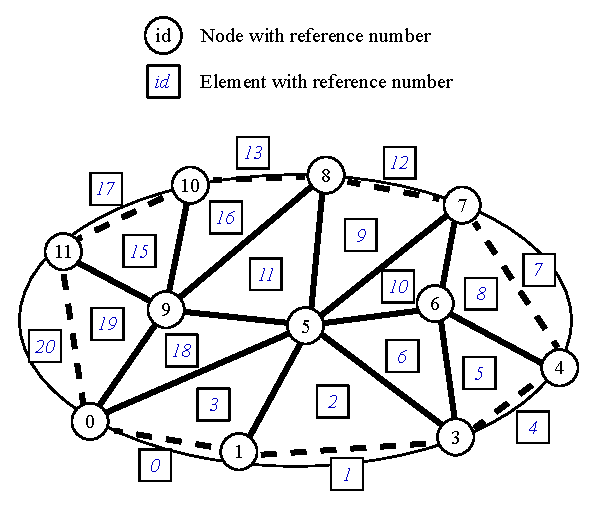
\includegraphics[width=\figwidth]{figures/FinleyMesh.eps}}
\caption{Subdivision of an Ellipse into triangles order 1 (\finleyelement{Tri3})}
\label{FINLEY FIG 0}
\end{figure}

\begin{figure}
\centerline{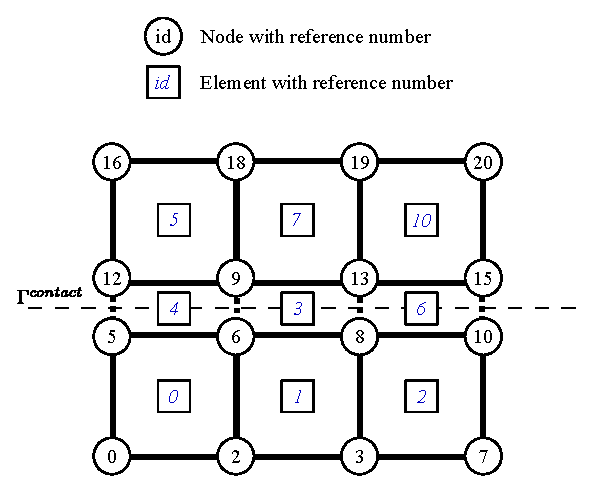
\includegraphics[width=\figwidth]{figures/FinleyContact.eps}}
\caption{Mesh around a contact region (\finleyelement{Rec4})}
\label{FINLEY FIG 01}
\end{figure}

\declaremodule{extension}{finley} \modulesynopsis{Solving linear, steady partial differential equations using
finite elements}

{\it finley} is a library of C functions solving linear, steady partial differential equations
\index{partial differential equations} (PDEs) or systems of PDEs using isoparametrical finite 
elements \index{FEM!isoparametrical}.
It supports unstructured, 1D, 2D and 3D meshes. The module \finley provides an access to the
library through the \LinearPDE class of \escript supporting its full functionality. {\it finley} 
is parallelized using the OpenMP \index{OpenMP} paradigm. 

\section{Formulation}

For a single PDE with a solution with a single component the linear PDE is defined in the
following form:
\begin{equation}\label{FINLEY.SINGLE.1}
\begin{array}{cl} &
\displaystyle{
\int\hackscore{\Omega} 
A\hackscore{jl} \cdot v\hackscore{,j}u\hackscore{,l}+ B\hackscore{j} \cdot v\hackscore{,j} u+ C\hackscore{l} \cdot v u\hackscore{,l}+D \cdot vu \; d\Omega }  \\
+ & \displaystyle{\int\hackscore{\Gamma} d \cdot vu \; d{\Gamma} } 
+  \displaystyle{\int\hackscore{\Gamma^{contact}} d^{contact} \cdot [v][u] \; d{\Gamma} } \\
= & \displaystyle{\int\hackscore{\Omega}  X\hackscore{j} \cdot v\hackscore{,j}+ Y \cdot v \; d\Omega }\\ 
+ & \displaystyle{\int\hackscore{\Gamma} y \cdot v \; d{\Gamma}}  + 
\displaystyle{\int\hackscore{\Gamma^{contact}} y^{contact}\cdot [v] \; d{\Gamma}} \\
\end{array}
\end{equation}

\section{Meshes}
To understand the usage of \finley one needs to have an understanding of how the finite element meshes
\index{FEM!mesh} are defined. \fig{FINLEY FIG 0} shows an example of the
subdivision of an ellipse into so called elements \index{FEM!elements} \index{element}. 
In this case, triangles have been used but other forms of subdivisions
can be constructed, e.g. into quadrilaterals or, in the three dimensional case, into tetrahedrons
and hexahedrons. The idea of the finite element method is to approximate the solution by a function
which is a polynomial of a certain order and is continuous across it boundary to neighbour elements.
In the example of \fig{FINLEY FIG 0} a linear polynomial is used on each triangle. As one can see, the triangulation
is quite a poor approximation of the ellipse. It can be improved by introducing a midpoint on each element edge then
positioning those nodes located on an edge expected to describe the boundary, onto the boundary.
In this case the triangle gets a curved edge which requires a parametrization of the triangle using a 
quadratic polynomial. For this case, the solution is also approximated by a piecewise quadratic polynomial
(which explains the name isoparametrical elements), see \Ref{Zienc,NumHand} for more details.   

The union of all elements defines the domain of the PDE.
Each element is defined by the nodes used to describe its shape. In \fig{FINLEY FIG 0} the element,
which has type \finleyelement{Tri3},
with element reference number $19$ \index{element!reference number} is defined by the nodes
with reference numbers $9$, $11$ and $0$ \index{node!reference number}. Notice that the order is counterclockwise. 
The coefficients of the PDE are evaluated at integration nodes with each individual element. 
For quadrilateral elements a Gauss quadrature scheme is used. In the case of triangular elements a 
modified form is applied. The boundary of the domain is also subdivided into elements. \index{element!face} In \fig{FINLEY FIG 0}
line elements with two nodes are used. The elements are also defined by their describing nodes, e.g.
the face element reference number $20$ which has type \finleyelement{Line2} is defined by the nodes
with the reference numbers $11$ and $0$. Again the order is crucial, if moving from the first
to second node the domain has to lie on the left hand side (in the case of a two dimension surface element
the domain has to lie on the left hand side when moving counterclockwise). If the gradient on the
surface of the domain is to be calculated rich face elements face to be used. Rich elements on a face
are identical to interior elements but with a modified order of nodes such that the 'first' face of the element aligns
with the surface of the domain. In \fig{FINLEY FIG 0}
elements of the type \finleyelement{Tri3Face} are used. 
The face element reference number $20$ as a rich face element is defined by the nodes
with reference numbers $11$, $0$ and $9$. Notice that the face element $20$ is identical to the
interior element $19$ except that, in this case, the order of the node is different to align the first
edge of the triangle (which is the edge starting with the first node) with the boundary of the domain.

Be aware that face elements and elements in the interior of the domain must match, i.e. a face element must be the face
of an interior element or, in case of a rich face element, it must be identical to an interior element.
If no face elements are specified
\finley implicitly assumes homogeneous natural boundary conditions \index{natural boundary conditions!homogeneous},
i.e. \var{d}=$0$ and \var{y}=$0$, on the entire boundary of the domain. For  
inhomogeneous natural boundary conditions \index{natural boundary conditions!inhomogeneous}, 
the boundary must be described by face elements. 

If discontinuities of the PDE solution are considered contact elements 
\index{element!contact}\index{contact conditions} are introduced to describe the contact region $\Gamma^{contact}$ 
even if $d^{contact}$ and $y^{contact}$ are zero. \fig{FINLEY FIG 01} shows a simple example of a mesh
of rectangular elements around a contact region $\Gamma^{contact}$ \index{element!contact}. 
The contact region is described by the
elements $4$, $3$ and $6$. Their element type is \finleyelement{Line2_Contact}. 
The nodes $9$, $12$, $6$, $5$ define contact element $4$, where the coordinates of nodes $12$ and $5$ and
nodes $4$ and $6$ are identical with the idea that nodes $12$ and $9$ are located above and 
nodes $5$ and $6$ below the contact region.  
Again, the order of the nodes within an element is crucial. There is also the option of using rich elements
if the gradient is to be calculated on the contact region. Similarly to the rich face elements 
these are constructed from two interior elements by reordering the nodes such that
the 'first' face of the element above and the 'first' face of the element below the 
contact regions line up.  The rich version of element 
$4$ is of type \finleyelement{Rec4Face_Contact} and is defined by the nodes $9$, $12$, $16$, $18$, $6$, $5$, $0$ and 
$2$.

\tab{FINLEY TAB 1} shows the interior element types and the corresponding element types to be used
on the face and contacts. \fig{FINLEY.FIG:1}, \fig{FINLEY.FIG:2} and \fig{FINLEY.FIG:4} show the ordering of
the nodes within an element.

\begin{table}
\begin{tablev}{l|llll}{textrm}{interior}{face}{rich face}{contact}{rich contact}
\linev{\finleyelement{Line2}}{\finleyelement{Point1}}{\finleyelement{Line2Face}}{\finleyelement{Point1_Contact}}{\finleyelement{Line2Face_Contact}}
\linev{\finleyelement{Line3}}{\finleyelement{Point1}}{\finleyelement{Line3Face}}{\finleyelement{Point1_Contact}}{\finleyelement{Line3Face_Contact}}
\linev{\finleyelement{Tri3}}{\finleyelement{Line2}}{\finleyelement{Tri3Face}}{\finleyelement{Line2_Contact}}{\finleyelement{Tri3Face_Contact}}
\linev{\finleyelement{Tri6}}{\finleyelement{Line3}}{\finleyelement{Tri6Face}}{\finleyelement{Line3_Contact}}{\finleyelement{Tri6Face_Contact}}
\linev{\finleyelement{Rec4}}{\finleyelement{Line2}}{\finleyelement{Rec4Face}}{\finleyelement{Line2_Contact}}{\finleyelement{Rec4Face_Contact}}
\linev{\finleyelement{Rec8}}{\finleyelement{Line3}}{\finleyelement{Rec8Face}}{\finleyelement{Line3_Contact}}{\finleyelement{Rec8Face_Contact}}
\linev{\finleyelement{Rec9}}{\finleyelement{Line3}}{\finleyelement{Rec9Face}}{\finleyelement{Line3_Contact}}{\finleyelement{Rec9Face_Contact}}
\linev{\finleyelement{Tet4}}{\finleyelement{Tri6}}{\finleyelement{Tet4Face}}{\finleyelement{Tri6_Contact}}{\finleyelement{Tet4Face_Contact}}
\linev{\finleyelement{Tet10}}{\finleyelement{Tri9}}{\finleyelement{Tet10Face}}{\finleyelement{Tri9_Contact}}{\finleyelement{Tet10Face_Contact}}
\linev{\finleyelement{Hex8}}{\finleyelement{Rec4}}{\finleyelement{Hex8Face}}{\finleyelement{Rec4_Contact}}{\finleyelement{Hex8Face_Contact}}
\linev{\finleyelement{Hex20}}{\finleyelement{Rec8}}{\finleyelement{Hex20Face}}{\finleyelement{Rec8_Contact}}{\finleyelement{Hex20Face_Contact}}
\end{tablev}
\caption{Finley elements and corresponding elements to be used on domain faces and contacts.
The rich types have to be used if the gradient of function is to be calculated on faces and contacts, respectively.}
\label{FINLEY TAB 1}
\end{table}

The native \finley file format is defined as follows.
Each node \var{i} has \var{dim} spatial coordinates \var{Node[i]}, a reference number
\var{Node_ref[i]}, a degree of freedom \var{Node_DOF[i]} and tag \var{Node_tag[i]}.
In most cases \var{Node_DOF[i]}=\var{Node_ref[i]} however, for periodic boundary conditions,
\var{Node_DOF[i]} is chosen differently, see example below. The tag can be used to mark nodes sharing
the same properties. Element \var{i} is defined by the \var{Element_numNodes} nodes \var{Element_Nodes[i]}
which is a list of node reference numbers. The order is crucial.
It has a reference number \var{Element_ref[i]} and a tag \var{Element_tag[i]}. The tag 
can be used to mark elements  sharing the same properties. For instance elements above 
a contact region are marked with $2$ and elements below a contact region are marked with $1$. 
\var{Element_Type} and \var{Element_Num} give the element type and the number of elements in the mesh.
Analogue notations are used for face and contact elements. The following Python script
prints the mesh definition in the \finley file format:
\begin{python}
print "%s\n"%mesh_name
# node coordinates:
print "%dD-nodes %d\n"%(dim,numNodes)
for i in range(numNodes): 
   print "%d %d %d"%(Node_ref[i],Node_DOF[i],Node_tag[i])
   for j in range(dim): print " %e"%Node[i][j]
   print "\n"
# interior elements
print "%s %d\n"%(Element_Type,Element_Num)
for i in range(Element_Num):
   print "%d %d"%(Element_ref[i],Element_tag[i])
   for j in range(Element_numNodes): print " %d"%Element_Nodes[i][j]
   print "\n"
# face elements
print "%s %d\n"%(FaceElement_Type,FaceElement_Num)
for i in range(FaceElement_Num):
   print "%d %d"%(FaceElement_ref[i],FaceElement_tag[i])
   for j in range(FaceElement_numNodes): print " %d"%FaceElement_Nodes[i][j]
   print "\n"
# contact elements
print "%s %d\n"%(ContactElement_Type,ContactElement_Num)
for i in range(ContactElement_Num):
   print "%d %d"%(ContactElement_ref[i],ContactElement_tag[i])
   for j in range(ContactElement_numNodes): print " %d"%ContactElement_Nodes[i][j]
   print "\n"
# point sources (not supported yet)
write("Point1 0",face_element_type,numFaceElements)
\end{python}

The following example of a mesh file defines the mesh shown in \fig{FINLEY FIG 01}:
\begin{verbatim}
Example 1
2D Nodes 16
0   0 0 0.   0.
2   2 0 0.33 0.
3   3 0 0.66 0.
7   4 0 1.   0.
5   5 0 0.   0.5
6   6 0 0.33 0.5
8   8 0 0.66 0.5
10 10 0 1.0  0.5
12 12 0 0.   0.5
9   9 0 0.33 0.5
13 13 0 0.66 0.5
15 15 0 1.0  0.5
16 16 0 0.   1.0
18 18 0 0.33 1.0
19 19 0 0.66 1.0
20 20 0 1.0  1.0
Rec4 6
 0 1  0  2  6  5
 1 1  2  3  8  6
 2 1  3  7 10  8
 5 2 12  9 18 16
 7 2 13 19 18  9
10 2 20 19 13 15
Line2 0
Line2_Contact 3
 4 0  9 12  6 5
 3 0 13  9  8 6
 6 0 15 13 10 8
Point1 0
\end{verbatim}
Notice that the order in which the nodes and elements are given is arbitrary.
In the case that rich contact elements are used the contact element section gets
 the form
\begin{verbatim}
Rec4Face_Contact 3
 4 0  9 12 16 18  6  5  0  2
 3 0 13  9 18 19  8  6  2  3
 6 0 15 13 19 20 10  8  3  7
\end{verbatim}
Periodic boundary condition \index{boundary conditions!periodic} can be introduced by altering \var{Node_DOF}.
It allows identification of nodes even if they have different physical locations. For instance, to
enforce periodic boundary conditions at the face $x_0=0$ and $x_0=1$ one identifies
the degrees of freedom for nodes $0$, $5$, $12$ and $16$ with the degrees of freedom for
$7$, $10$, $15$ and $20$, respectively. The node section of the \finley mesh gets now the form:  
\begin{verbatim}
2D Nodes 16
0   0 0 0.   0.
2   2 0 0.33 0.
3   3 0 0.66 0.
7   0 0 1.   0.
5   5 0 0.   0.5
6   6 0 0.33 0.5
8   8 0 0.66 0.5
10  5 0 1.0  0.5
12 12 0 0.   0.5
9   9 0 0.33 0.5
13 13 0 0.66 0.5
15 12 0 1.0  0.5
16 16 0 0.   1.0
18 18 0 0.33 1.0
19 19 0 0.66 1.0
20 16 0 1.0  1.0
\end{verbatim}



%%%%%%%%%%%%%%%%%%%%%%%%%%%%%%%%%%%%%%%%%%%%%%%%%%%%%%%%%%%%%%%%%%%%%%%%%%%%%%
% Copyright (c) 2003-2018 by The University of Queensland
% http://www.uq.edu.au
%
% Primary Business: Queensland, Australia
% Licensed under the Apache License, version 2.0
% http://www.apache.org/licenses/LICENSE-2.0
%
% See CREDITS file for contributors and development history
%
%%%%%%%%%%%%%%%%%%%%%%%%%%%%%%%%%%%%%%%%%%%%%%%%%%%%%%%%%%%%%%%%%%%%%%%%%%%%%%

\setlength{\unitlength}{1mm}

\newsavebox{\HLa}
\savebox{\HLa}(0,0)
  {\put(0,0){\circle*{2}}
   \thicklines \put(1,0){\line(1,0){28}}
   \put(30,0){\circle*{2}} }

\newsavebox{\HLathin}
\savebox{\HLathin}(0,0)
  {\put(0,0){\circle{2}}
   \thinlines \put(1,0){\line(1,0){28}}
   \put(30,0){\circle{2}} }

\newsavebox{\VLa}
\savebox{\VLa}(0,30)
  {\put(0,0){\circle*{2}}
   \thicklines \put(0,1){\line(0,1){28}}
   \put(0,30){\circle*{2}} }

\newsavebox{\VLathin}
\savebox{\VLathin}(0,30)
  {\put(0,0){\circle{2}}
   \thinlines \put(0,1){\line(0,1){28}}
   \put(0,30){\circle{2}} }

\newsavebox{\SLax}
\savebox{\SLax}(0,30)
  {\thicklines \put(0,0){\line(-1,1){30}}
   \put(0,0){\circle*{2}}
   \put(-30,30){\circle*{2}} }

\newsavebox{\SLaa}
\savebox{\SLaa}(0,15)
  {\thicklines \put(0,0){\line(-4,3){20}}
   \put(0,0){\circle*{2}}
   \put(-20,15){\circle*{2}} }

\newsavebox{\SLab}
\savebox{\SLab}(0,-15)
  {\thicklines \put(0,0){\line(-4,-3){20}}
   \put(0,0){\circle*{2}}
   \put(-20,-15){\circle*{2}} }

\newsavebox{\SLabthin}
\savebox{\SLabthin}(0,-15)
  {\thinlines \put(-0.7,-0.7){\line(-4,-3){18.7}}
   \put(0,0){\circle{2}}
   \put(-20,-15){\circle{2}} }

\newsavebox{\SLac}
\savebox{\SLac}(0,15)
  {\thicklines \put(0,0){\line(-2,3){10}}
   \put(0,0){\circle*{2}}
   \put(-10,15){\circle*{2}} }

\newsavebox{\SLacthin}
\savebox{\SLacthin}(0,15)
  {\thinlines \put(0,0){\line(-2,3){9.4}}
   \put(0,0){\circle{2}}
   \put(-10,15){\circle{2}} }


\newsavebox{\HLd}
\savebox{\HLd}(0,0)
  {\put(0,0){\circle*{2}}
   \put(10,0){\circle*{2}}
   \thicklines \put(1,0){\line(1,0){28}}
   \put(20,0){\circle*{2}}
   \put(30,0){\circle*{2}} }

\newsavebox{\HLdthin}
\savebox{\HLdthin}(0,0)
  {\put(0,0){\circle{2}}
   \put(10,0){\circle{2}}
   \thinlines \multiput(1,0)(10,0){3}{\line(1,0){8}}
   \put(20,0){\circle{2}}
   \put(30,0){\circle{2}} }

\newsavebox{\VLd}
\savebox{\VLd}(0,30)
  {\put(0,0){\circle*{2}}
   \put(0,10){\circle*{2}}
   \thicklines \put(0,1){\line(0,1){28}}
   \put(0,20){\circle*{2}}
   \put(0,30){\circle*{2}} }

\newsavebox{\VLdthin}
\savebox{\VLdthin}(0,30)
  {\put(0,0){\circle{2}}
   \put(0,10){\circle{2}}
   \thinlines \multiput(0,1)(0,10){3}{\line(0,1){8}}
   \put(0,20){\circle{2}}
   \put(0,30){\circle{2}} }

\newsavebox{\SLf}
\savebox{\SLf}(0,30)
  {\thicklines \put(0,0){\line(-1,1){30}}
   \put(0,0){\circle*{2}}
   \put(-10,10){\circle*{2}}
   \put(-20,20){\circle*{2}}
   \put(-30,30){\circle*{2}} }

\newsavebox{\SLad}
\savebox{\SLad}(0,15)
  {\thicklines \put(0,0){\line(-4,3){20}}
   \put(0,0){\circle*{2}}
   \put(-6.66,5){\circle*{2}}
   \put(-13.33,10){\circle*{2}}
   \put(-20,15){\circle*{2}} }

\newsavebox{\SLbd}
\savebox{\SLbd}(0,-15)
  {\thicklines \put(0,0){\line(-4,-3){20}}
   \put(0,0){\circle*{2}}
   \put(-6.66,-5){\circle*{2}}
   \put(-13.33,-10){\circle*{2}}
   \put(-20,-15){\circle*{2}} }

\newsavebox{\SLbdthin}
\savebox{\SLbdthin}(0,-15)
  {\thinlines \multiput(-0.7,-0.7)(-6.66,-5){3}{\line(-4,-3){5.1}}
   \put(0,0){\circle{2}}
   \put(-6.66,-5){\circle{2}}
   \put(-13.33,-10){\circle{2}}
   \put(-20,-15){\circle{2}} }

\newsavebox{\SLcd}
\savebox{\SLcd}(0,15)
  {\thicklines \put(0,0){\line(-2,3){10}}
   \put(0,0){\circle*{2}}
   \put(-3.33,5){\circle*{2}}
   \put(-6.66,10){\circle*{2}}
   \put(-10,15){\circle*{2}} }

\newsavebox{\SLcdthin}
\savebox{\SLcdthin}(0,15)
  {\thinlines \multiput(-0.6,0.8)(-3.33,5){3}{\line(-2,3){2.35}}
   \put(0,0){\circle{2}}
   \put(-3.33,5){\circle{2}}
   \put(-6.66,10){\circle{2}}
   \put(-10,15){\circle{2}} }

\newsavebox{\HLe}
\savebox{\HLe}(0,0)
  {\put(0,0){\circle*{2}}
   \put(15,0){\circle*{2}}
   \thicklines \put(1,0){\line(1,0){28}}
   \put(30,0){\circle*{2}} }

\newsavebox{\HLethin}
\savebox{\HLethin}(0,0)
  {\put(0,0){\circle{2}}
   \put(15,0){\circle{2}}
   \thinlines \multiput(1,0)(15,0){2}{\line(1,0){13}}
   \put(30,0){\circle{2}} }

\newsavebox{\VLe}
\savebox{\VLe}(0,30)
  {\put(0,0){\circle*{2}}
   \put(0,15){\circle*{2}}
   \thicklines \put(0,1){\line(0,1){28}}
   \put(0,30){\circle*{2}} }

\newsavebox{\VLethin}
\savebox{\VLethin}(0,30)
  {\put(0,0){\circle{2}}
   \put(0,15){\circle{2}}
   \thinlines \multiput(0,1)(0,15){2}{\line(0,1){13}}
   \put(0,30){\circle{2}} }

\newsavebox{\SLe}
\savebox{\SLe}(0,30)
  {\thicklines \put(0,0){\line(-1,1){30}}
   \put(0,0){\circle*{2}}
   \put(-15,15){\circle*{2}}
   \put(-30,30){\circle*{2}} }

\newsavebox{\SLae}
\savebox{\SLae}(0,15)
  {\thicklines \put(0,0){\line(-4,3){20}}
   \put(0,0){\circle*{2}}
   \put(-10,7.5){\circle*{2}}
   \put(-20,15){\circle*{2}} }

\newsavebox{\SLbe}
\savebox{\SLbe}(0,-15)
  {\thicklines \put(0,0){\line(-4,-3){20}}
   \put(0,0){\circle*{2}}
   \put(-10,-7.5){\circle*{2}}
   \put(-20,-15){\circle*{2}} }

\newsavebox{\SLbethin}
\savebox{\SLbethin}(0,-15)
  {\thinlines \multiput(-0.7,-0.7)(-10,-7.5){2}{\line(-4,-3){8.4}}
   \put(0,0){\circle{2}}
   \put(-10,-7.5){\circle{2}}
   \put(-20,-15){\circle{2}} }

\newsavebox{\SLce}
\savebox{\SLce}(0,15)
  {\thicklines \put(0,0){\line(-2,3){10}}
   \put(0,0){\circle*{2}}
   \put(-5,7.5){\circle*{2}}
   \put(-10,15){\circle*{2}} }

\newsavebox{\SLcethin}
\savebox{\SLcethin}(0,15)
  {\thinlines \multiput(-0.6,0.8)(-5,7.5){2}{\line(-2,3){3.9}}
   \put(0,0){\circle{2}}
   \put(-5,7.5){\circle{2}}
   \put(-10,15){\circle{2}} }

%=====================================================================
%
%   order 1
%   -------
%

\begin{figure}
\begin{center}
\begin{picture}(150,160) \thicklines

\put(20,155){\circle*{2}}
\put(15,145){\parbox[t]{45mm}
             \finleyelement{Point1}}

\put(90,155){\usebox{\HLa}}
\put(90,145){\parbox[t]{45mm}
             \finleyelement{Line2} }

\put(10,95){\usebox{\HLa}}
\put(40,95){\usebox{\SLax}}
\put(10,95){\usebox{\VLa}}
\put(10,85){\parbox[t]{45mm}
             \finleyelement{Tri3} }

\put(90,95){\usebox{\HLa}}
\put(90,125){\usebox{\HLa}}
\put(90,95){\usebox{\VLa}}
\put(120,95){\usebox{\VLa}}
\put(90,85){\parbox[t]{45mm}
             \finleyelement{Rec4} }

\put(10,20){\usebox{\HLa}}
\put(40,20){\usebox{\SLax}}
\put(10,20){\usebox{\VLa}}
\put(40,20){\usebox{\SLac}}
\put(30,35){\usebox{\SLabthin}}
\put(30,35){\usebox{\SLaa}}
\put(10,10 ){\parbox[t]{45mm}
             \finleyelement{Tet4} }

\put(90,20){\usebox{\HLa}}
\put(90,50){\usebox{\HLa}}
\put(90,20){\usebox{\VLa}}
\put(120,20){\usebox{\VLa}}
\put(110,35){\usebox{\SLabthin}}
\put(140,35){\usebox{\SLab}}
\put(110,65){\usebox{\SLab}}
\put(140,65){\usebox{\SLab}}
\put(110,35){\usebox{\HLathin}}
\put(110,65){\usebox{\HLa}}
\put(110,35){\usebox{\VLathin}}
\put(140,35){\usebox{\VLa}}
\put(90,10 ){\parbox[t]{45mm}
             \finleyelement{Hex8} }

% numbering the lines:
 % Point
\put(19,158){{\it 1}}
% line
\put(89,158){{\it 1}} 
\put(119,158){{\it 2}}
% Triangle
\put(6,124){{\it 3}}
\put(6,94){{\it 1}}
\put(43,94){{\it 2}}
% quadrilateral
\put(86,124){{\it 4}}
\put(86,94){{\it 1}}
\put(123,124){{\it 3}}
\put(123,94){{\it 2}}
% Tetrahedron
\put(6,49){{\it 4}}
\put(6,19){{\it 1}}
\put(43,19){{\it 2}}
\put(33,34){{\it 3}}
% Hexahedron
\put(86,49){{\it 5}} 
\put(86,19){{\it 1}}
\put(123,49){{\it 6}}
\put(123,19){{\it 2}}
\put(106,64){{\it 8}}
\put(106,34){{\it 4}}
\put(143,64){{\it 7}}
\put(143,34){{\it 3}}
\end{picture}
\caption{\label{FINLEY.FIG:1} Elements of order 1}
\end{center}
\end{figure}
%=====================================================================
%
%
%   order 2
%   -------
%   (boxes in 'fesubelm')


\begin{figure}
\begin{center}
\setlength{\unitlength}{1mm}
\begin{picture}(150,160) \thicklines

\put(20,155){\circle*{2}}
\put(15,145){\parbox[t]{45mm}
             \finleyelement{Point1} }

\put(90,155){\usebox{\HLe}}
\put(90,145){\parbox[t]{45mm}
             \finleyelement{Line3} and \finleyelement{Line3Macro} }

\put(10,95){\usebox{\HLe}}
\put(40,95){\usebox{\SLe}}
\put(10,95){\usebox{\VLe}}
\put(10,85){\parbox[t]{45mm}
             \finleyelement{Tri6} }

\put(90,95){\usebox{\HLe}}
\put(90,125){\usebox{\HLe}}
\put(90,95){\usebox{\VLe}}
\put(120,95){\usebox{\VLe}}
\put(90,85){\parbox[t]{45mm}
             \finleyelement{Rec8} }

\put(10,20){\usebox{\HLe}}
\put(40,20){\usebox{\SLe}}
\put(10,20){\usebox{\VLe}}
\put(40,20){\usebox{\SLce}}
\put(30,35){\usebox{\SLbethin}}
\put(30,35){\usebox{\SLae}}
\put(10,10 ){\parbox[t]{45mm}
             \finleyelement{Tet10} and \finleyelement{Tet10Macro}}

\put(90,20){\usebox{\HLe}}
\put(90,50){\usebox{\HLe}}
\put(90,20){\usebox{\VLe}}
\put(120,20){\usebox{\VLe}}
\put(110,35){\usebox{\SLbethin}}
\put(140,35){\usebox{\SLbe}}
\put(110,65){\usebox{\SLbe}}
\put(140,65){\usebox{\SLbe}}
\put(110,35){\usebox{\HLethin}}
\put(110,65){\usebox{\HLe}}
\put(110,35){\usebox{\VLethin}}
\put(140,35){\usebox{\VLe}}
\put(90,10 ){\parbox[t]{45mm}
             \finleyelement{Hex20} }


% numbering the lines:
% Point
\put(19,158){{\it 1}} 
% line
\put(89,158){{\it 1}} 
\put(104,158){{\it 3}}
\put(119,158){{\it 2}}
% Triangle
\put(6,124){{\it 3}} 
\put(6,109){{\it 6}}
\put(6,94){{\it 1}}
\put(28,109){{\it 5}}
\put(43,94){{\it 2}}
\put(24,90){{\it 4}}
% quaTrilateral
\put(104,90){{\it 5}} 
\put(86,124){{\it 4}}
\put(86,109){{\it 8}}
\put(86,94){{\it 1}}
\put(104,128){{\it 7}}
\put(123,124){{\it 3}}
\put(123,109){{\it 6}}
\put(123,94){{\it 2}}
% Tetrahedron
\put(24,15){{\it 5}} 
\put(6,49){{\it 4}}
\put(6,34){{\it 8}}
\put(6,19){{\it 1}}
\put(21,34){{\it 9}}
\put(43,19){{\it 2}}
\put(16,26.5){{\it 7}}
\put(38,26.5){{\it 6}}
\put(33,34){{\it 3}}
\put(22.5,41.5){{\it 10}}
% Hexahedron
\put(104,15){{\it 9}} 
\put(86,49){{\it 5}}
\put(85,34){{\it 13}}
\put(86,19){{\it 1}}
\put(104,52){{\it 17}}
\put(123,49){{\it 6}}
\put(115,37){{\it 14}}
\put(123,19){{\it 2}}
\put(125,37){{\it 11}}
\put(106,64){{\it 8}}
\put(112,46){{\it 16}}
\put(106,34){{\it 4}}
\put(124,68){{\it 19}}
\put(143,64){{\it 7}}
\put(142,49){{\it 15}}
\put(143,34){{\it 3}}
\put(94.5,26.5){{\it 12}}
\put(132.5,26.5){{\it 10}}
\put(94.5,56.5){{\it 20}}
\put(132.5,56.5){{\it 18}}

\end{picture}
\caption{\label{FINLEY.FIG:2} Elements of order 2 and macro elements}
\end{center}
\end{figure}

%
% additional elements
%
\begin{figure}
\begin{center}
\begin{picture}(50,50) \thicklines
\put(10,10){\usebox{\HLe}}
\put(10,40){\usebox{\HLe}}
\put(10,10){\usebox{\VLe}}
\put(40,10){\usebox{\VLe}}
\put(25,25){\circle*{2}}
% \put(50,085){\parbox[t]{45mm}
%              \finleyelement{Rec9} and  \finleyelement{Rec9Macro}}
\put(24,5){{\it 5}}
\put(6,39){{\it 4}}
\put(6,24){{\it 8}}
\put(6,9){{\it 1}}
\put(24,43){{\it 7}}
\put(43,43){{\it 3}}
\put(43,25){{\it 6}}
\put(43,9){{\it 2}}
\put(24,20){{\it 9}}
\end{picture}
\caption{\label{FINLEY.FIG:4}\finleyelement{Rec9} and  \finleyelement{Rec9Macro}}
\end{center}
\end{figure}


\subsection{Linear Solvers in \LinearPDE}
Currently \finley supports the linear solvers \PCG, \GMRES, \PRESTWENTY and \BiCGStab. 
For \GMRES the options \var{truncation} and \var{restart} of the \method{getSolution} can be
used to control the truncation and restart during iteration. Default values are
\var{truncation}=5 and \var{restart}=20.
The default solver is \BiCGStab  but if the symmetry flag is set \PCG is the default solver.
\finley supports the solver options \var{iter_max} which specifies the maximum number of iterations steps,
\var{verbose}=\True or \False and \var{preconditioner}=\constant{JACOBI} or \constant {ILU0}.
In some installations \finley supports the \Direct solver and the
solver options \var{reordering}=\constant{util.NO_REORDERING}, 
\constant{util.MINIMUM_FILL_IN} or \constant{util.NESTED_DISSECTION} (default is \constant{util.NO_REORDERING}),
\var{drop_tolerance} specifying the threshold for values to be dropped in the 
incomplete elimination process (default is 0.01) and \var{drop_storage} specifying the maximum increase 
in storage allowed in the 
incomplete elimination process (default is 1.20).

\subsection{Functions}
\begin{funcdesc}{Mesh}{fileName,integrationOrder=-1}
creates a \Domain object form the FEM mesh defined in 
file \var{fileName}. The file must be given the \finley file format.
If \var{integrationOrder} is positive, a numerical integration scheme
chosen which is accurate on each element up to a polynomial of
degree \var{integrationOrder} \index{integration order}. Otherwise
an appropriate integration order is chosen independently.
\end{funcdesc}

\begin{funcdesc}{Rectangle}{n0,n1,order=1,l0=1.,l1=1., integrationOrder=-1, \\
  periodic0=\False,periodic1=\False,useElementsOnFace=\False,optimize=\False}
Generates a \Domain object representing a two dimensional rectangle between
$(0,0)$ and $(l0,l1)$ with orthogonal edges. The rectangle is filled with
\var{n0} elements along the $x_0$-axis and
\var{n1} elements along the $x_1$-axis. 
For \var{order}=1 and \var{order}=2
\finleyelement{Rec4} and  
\finleyelement{Rec8} are used, respectively. 
In the case of \var{useElementsOnFace}=\False,
\finleyelement{Line2} and  
\finleyelement{Line3} are used to subdivide the edges of the rectangle, respectively. 
In the case of \var{useElementsOnFace}=\True (this option should be used if gradients
are calculated on domain faces),
\finleyelement{Rec4Face} and  
\finleyelement{Rec8Face} are used on the edges, respectively.  
If \var{integrationOrder} is positive, a numerical integration scheme
chosen which is accurate on each element up to a polynomial of
degree \var{integrationOrder} \index{integration order}. Otherwise
an appropriate integration order is chosen independently. If
\var{periodic0}=\True, periodic boundary conditions \index{periodic boundary conditions}
along the $x_0$-directions are enforced. That means when for any solution of a PDE solved by \finley
the value on the line $x_0=0$ will be identical to the values on $x_0=\var{l0}$.
Correspondingly,
\var{periodic1}=\False sets periodic boundary conditions
in $x_1$-direction.
If \var{optimize}=\True mesh node relabeling will be attempted to reduce the computation and also ParMETIS will be used to improve the mesh partition if running on multiple CPUs with MPI.
\end{funcdesc}

\begin{funcdesc}{Brick}{n0,n1,n2,order=1,l0=1.,l1=1.,l2=1., integrationOrder=-1, \\
  periodic0=\False,periodic1=\False,periodic2=\False,useElementsOnFace=\False,optimize=\False}
Generates a \Domain object representing a three dimensional brick between
$(0,0,0)$ and $(l0,l1,l2)$ with orthogonal faces. The brick is filled with
\var{n0} elements along the $x_0$-axis, 
\var{n1} elements along the $x_1$-axis and 
\var{n2} elements along the $x_2$-axis. 
For \var{order}=1 and \var{order}=2
\finleyelement{Hex8} and  
\finleyelement{Hex20} are used, respectively. 
In the case of \var{useElementsOnFace}=\False,
\finleyelement{Rec4} and  
\finleyelement{Rec8} are used to subdivide the faces of the brick, respectively. 
In the case of \var{useElementsOnFace}=\True (this option should be used if gradients
are calculated on domain faces),
\finleyelement{Hex8Face} and  
\finleyelement{Hex20Face} are used on the brick faces, respectively.  
If \var{integrationOrder} is positive, a numerical integration scheme
chosen which is accurate on each element up to a polynomial of
degree \var{integrationOrder} \index{integration order}. Otherwise
an appropriate integration order is chosen independently. If
\var{periodic0}=\True, periodic boundary conditions \index{periodic boundary conditions}
along the $x_0$-directions are enforced. That means when for any solution of a PDE solved by \finley
the value on the plane $x_0=0$ will be identical to the values on $x_0=\var{l0}$. Correspondingly,
\var{periodic1}=\False and \var{periodic2}=\False sets periodic boundary conditions
in $x_1$-direction and $x_2$-direction, respectively.
If \var{optimize}=\True mesh node relabeling will be attempted to reduce the computation and also ParMETIS will be used to improve the mesh partition if running on multiple CPUs with MPI.
\end{funcdesc}

\begin{funcdesc}{GlueFaces}{meshList,safetyFactor=0.2,tolerance=1.e-13}
Generates a new \Domain object from the list \var{meshList} of \finley meshes.
Nodes in face elements whose difference of coordinates is less then \var{tolerance} times the 
diameter of the domain are merged. The corresponding face elements are removed from the mesh.  

TODO: explain \var{safetyFactor} and show an example.
\end{funcdesc}

\begin{funcdesc}{JoinFaces}{meshList,safetyFactor=0.2,tolerance=1.e-13}
Generates a new \Domain object from the list \var{meshList} of \finley meshes.
Face elements whose nodes coordinates have difference is less then \var{tolerance} times the 
diameter of the domain are combined to form a contact element \index{element!contact} 
The corresponding face elements are removed from the mesh.  

TODO: explain \var{safetyFactor} and show an example.
\end{funcdesc}


\input{troubleshooting}
\makemodindex

\printindex
%% $Id$
\documentclass{manual}

% grab the handy definitions and \usepackage statements etc
% $Id$

\usepackage{epsfig}
\usepackage{graphicx,color}
\usepackage{makeidx}  % handle the index properly
\usepackage{xspace}   % handle spaces after commands more nicely
% use the ams math stuff, as it makes the maths easier to code, and
% nicer output than the standard LaTeX stuff
\usepackage{amsmath,amsfonts,amssymb} % this is handy for mathematicians and physicists
			              % see http://www.ams.org/tex/amslatex.html
\usepackage{alltt}   % handy verbatim stuff


% define some handy commands for escript stuff
\newcommand{\ESyS}{\module{ESyS}\xspace}
\newcommand{\escript}{\module{escript}\xspace}
\newcommand{\finley}{\module{finley}\xspace}
\newcommand{\linearPDE}{\class{linearPDE}\xspace}
\newcommand{\Data}{\class{Data}\xspace}

% default width for figures
\newcommand{\figwidth}{100mm}

% commands useful in cross-referencing
\newcommand {\Ref}[1] {Reference~\cite{#1}}
\newcommand {\Sec}[1] {Section~\ref{#1}}
\newcommand {\App}[1] {Appendix~\ref{#1}}
\newcommand {\Chap}[1] {Chapter~\ref{#1}}
\newcommand {\etal} {\emph{~et~al.}}
\newcommand {\fig}[1] {Figure~\ref{#1}}
\newcommand {\eqn}[1] {Equation~(\ref{#1})} 
\newcommand {\tab}[1] {Table~\ref{#1}}

% improved version of caption handling
\usepackage{ccaption}
\captionnamefont{\scshape}
\captionstyle{}
\makeatletter
\renewcommand{\fnum@figure}[1]{\quad\small\textsc{\figurename~\thefigure}:}
\renewcommand{\@makecaption}[2]{%
\vskip\abovecaptionskip
\sbox\@tempboxa{#1: #2}%
\ifdim \wd\@tempboxa >\hsize
  \def\baselinestretch{1}\@normalsize
  #1: #2\par
  \def\baselinestretch{1.5}\@normalsize
\else
  \global \@minipagefalse
  \hb@xt@\hsize{\hfil\box\@tempboxa\hfil}%
\fi
\vskip\belowcaptionskip}
\makeatother

\usepackage{fancyvrb}  % fancy verbatim stuff.  Needed so code below goes
%%% this code grabbed from the PyScript docs
%%% pyscript.sourceforge.net

% --------------------------------------------------------------
% Code format within \Verb
% --------------------------------------------------------------

\definecolor{pycolor}{rgb}{0,0.4,0}

\DefineVerbatimEnvironment{python}{Verbatim}
{frame=leftline,framerule=.5mm,rulecolor=\color{pycolor},
formatcom=\color{pycolor}\small,fontshape=rm}

%\DefineShortVerb[formatcom=\color{dgreen}\small,fontshape=sl]{\|}

\RecustomVerbatimCommand{\Verb}{Verb}{formatcom=\color{pycolor}\small,fontshape=rm}

%%% end of grabbed code

% this is for when one uses pdflatex and therefore needs to load pdf
% figures into \includegraphics
\ifpdf
	\DeclareGraphicsExtensions{.pdf}  % this command defined in graphicx
	\pdfcompresslevel=9  % 0: no compression, 9: highest compression
			     % or, set compress_level 9 in file pdftex.cfg
\else
	\DeclareGraphicsExtensions{.eps}
\fi


% title, author, etc stuff
\title{ESyS Users Guide}

\author{Lutz Gross (Editor)}
\authoraddress{
Earth Systems Science Computational Centre (ESSCC) \\
The University of Queensland \\
Australia \\
Email: \email{esys@access.edu.au}
}                                                                                         
\date{\today}      
\release{$Id$}
\setreleaseinfo{} 
\setshortversion{}

\makeindex

% the actual start of the document
\begin{document}

\maketitle


%%%%%%%%%%%%%%%%%%%%%%%%%%%%%%%%%%%%%%%%%%%%%%%%%%%%%%%%%%%%%%%%%%%%%%%%%%%%%%
% Copyright (c) 2003-2026 by the esys.escript Group
% https://github.com/LutzGross/esys-escript.github.io
%
% Primary Business: Queensland, Australia
% Licensed under the Apache License, version 2.0
% http://www.apache.org/licenses/LICENSE-2.0
%
% See CREDITS file for contributors and development history
%
%%%%%%%%%%%%%%%%%%%%%%%%%%%%%%%%%%%%%%%%%%%%%%%%%%%%%%%%%%%%%%%%%%%%%%%%%%%%%%

\begin{center}
Copyright (c) 2003-2026 esys.escript Group \\
\url{https://github.com/LutzGross/esys-escript.github.io}\\
Primary Business: Queensland, Australia\\
Licensed under the Apache License, version 2.0\\
\url{http://www.apache.org/licenses/LICENSE-2.0}\\
This work was supported by the AuScope National Collaborative Research
Infrastructure Strategy, the Queensland State Government and The University
of Queensland.
\end{center}



\begin{abstract}
This document is a guide of how to use the \ESyS software and
associated tools.
\end{abstract}

\tableofcontents

% $Id$


\chapter{Introduction}
\label{INTRO}

\subsection{Getting the software}


\escript, \ESyS, all freely available.  Where do people get \finley from?



\begin{enumerate}
 \item general structure 
 \item how to get the software
 \item a few words about the general structure
\item installation
\end{enumerate}

\subsection{Acknowlegements}
\begin{itemize}
\item Margeret Kahn Australian Nationional Unversity, Canberra.
\end{itemize}


%%%%%%%%%%%%%%%%%%%%%%%%%%%%%%%%%%%%%%%%%%%%%%%%%%%%%%%%%%%%%%%%%%%%%%%%%%%%%%
% Copyright (c) 2003-2026 by the esys.escript Group
% https://github.com/LutzGross/esys-escript.github.io
%
% Primary Business: Queensland, Australia
% Licensed under the Apache License, version 2.0
% http://www.apache.org/licenses/LICENSE-2.0
%
% See CREDITS file for contributors and development history
%
%%%%%%%%%%%%%%%%%%%%%%%%%%%%%%%%%%%%%%%%%%%%%%%%%%%%%%%%%%%%%%%%%%%%%%%%%%%%%%

\section{The First Steps}\label{FirstSteps} 
This chapter is an introduction on how to use \escript to solve 
a partial differential equation\index{partial differential equation} (PDE\index{partial differential equation!PDE}).
We assume you are at least a little familiar with \PYTHON.
The knowledge presented in the \PYTHON tutorial at \url{https://docs.python.org/2/tutorial/} is more than sufficient.

The PDE\index{partial differential equation} we wish to solve is the Poisson equation\index{Poisson equation} 
\begin{equation}
    -\Delta u=f 
    \label{eq:FirstSteps.1}
\end{equation}
for the solution $u$. The function $f$ is the given right hand side. The domain of interest, denoted by $\Omega$,
is the unit square 
\begin{equation}
\Omega=[0,1]^2=\{ (x_0;x_1) | 0\le x_{0} \le 1 \mbox{ and } 0\le x_{1} \le 1 \}
\label{eq:FirstSteps.1b}
\end{equation}
The domain is shown in \fig{fig:FirstSteps.1}.
\begin{figure}[ht]
    \centerline{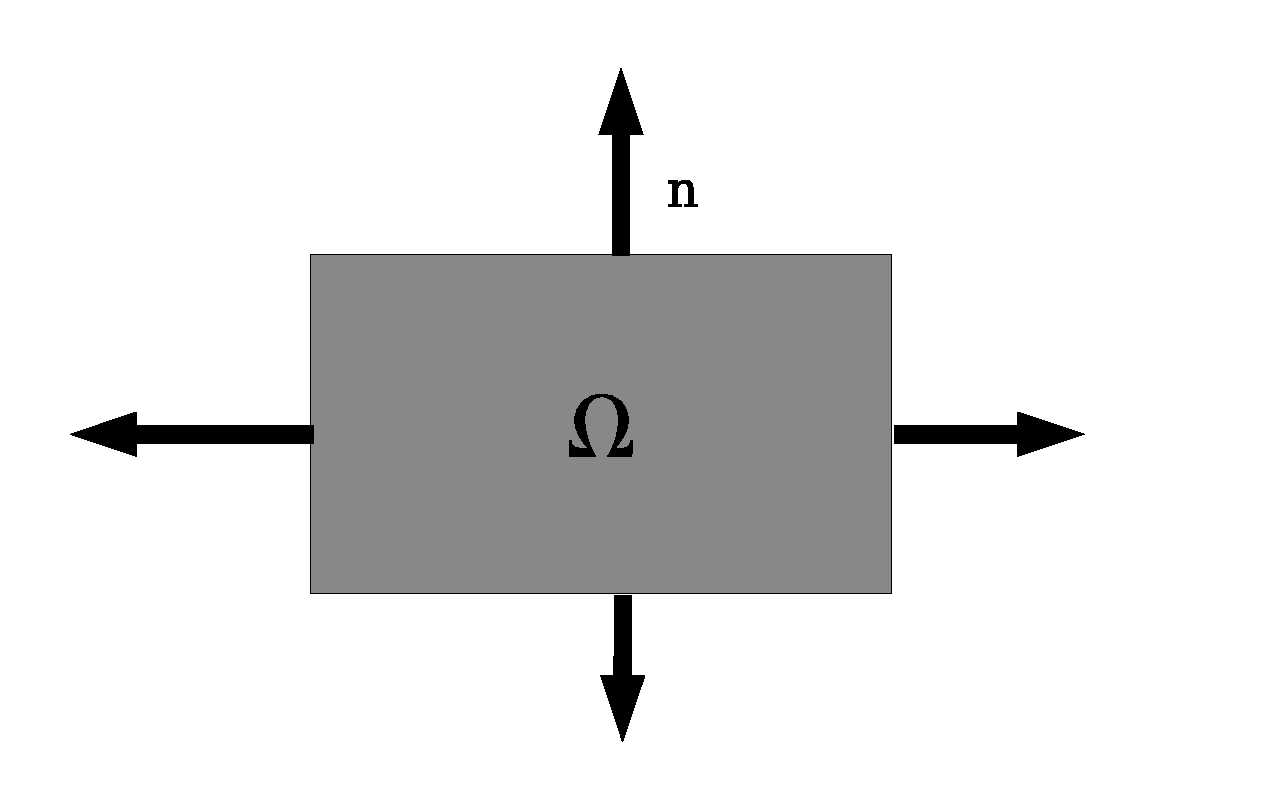
\includegraphics{FirstStepDomain}}
    \caption{Domain $\Omega=[0,1]^2$ with outer normal field $n$.}
    \label{fig:FirstSteps.1}
\end{figure}

$\Delta$ denotes the Laplace operator\index{Laplace operator}, which is defined by
\begin{equation}
\Delta u = (u_{,0})_{,0}+(u_{,1})_{,1}
\label{eq:FirstSteps.1.1}
\end{equation}
where, for any function $u$ and any direction $i$, $u_{,i}$
denotes the partial derivative \index{partial derivative} of $u$ with respect
to $i$.\footnote{You may be more familiar with the Laplace
operator\index{Laplace operator} being written as $\nabla^2$, and written in
the form
\begin{equation*}
    \nabla^2 u = \nabla^t \cdot \nabla u =  \frac{\partial^2 u}{\partial x_0^2} 
    + \frac{\partial^2 u}{\partial  x_1^2}
\end{equation*}
and \eqn{eq:FirstSteps.1} as
\begin{equation*}
    -\nabla^2 u = f
\end{equation*}
}
Basically, in the subindex of a function, any index to the right of the comma denotes a spatial derivative with respect 
to the index. To get a more compact form we will write $u_{,ij}=(u_{,i})_{,j}$
which leads to
\begin{equation}
\Delta u = u_{,00}+u_{,11}=\sum_{i=0}^2 u_{,ii}
\label{eq:FirstSteps.1.1b}
\end{equation}
We often find that use
of nested $\sum$ symbols makes formulas cumbersome, and we use the more
compact Einstein summation convention\index{summation convention}. This 
drops the $\sum$ sign and assumes that a summation is performed over any repeated index.
For instance, 
\begin{eqnarray}
x_{i}y_{i}=\sum_{i=0}^2 x_{i}y_{i}   \\
x_{i}u_{,i}=\sum_{i=0}^2 x_{i}u_{,i}   \\
u_{,ii}=\sum_{i=0}^2 u_{,ii} \\
x_{ij}u_{i,j}=\sum_{j=0}^2\sum_{i=0}^2 x_{ij}u_{i,j}   \\
\label{eq:FirstSteps.1.1c}
\end{eqnarray}
With the summation convention we can write the Poisson equation \index{Poisson equation} as
\begin{equation}
- u_{,ii} =1 
\label{eq:FirstSteps.1.sum}
\end{equation}
where $f=1$ in this example.

On the boundary of the domain $\Omega$ the normal derivative $n_{i} u_{,i}$
of the solution $u$ shall be zero, i.e. $u$ shall fulfill
the homogeneous Neumann boundary condition\index{Neumann
boundary condition!homogeneous}
\begin{equation}
n_{i} u_{,i}= 0 \;.
\label{eq:FirstSteps.2}
\end{equation}
$n=(n_{i})$ denotes the outer normal field
of the domain, see \fig{fig:FirstSteps.1}. Remember that we 
apply the Einstein summation convention \index{summation convention}, i.e. $n_{i} u_{,i}= n_{0} u_{,0} +%
n_{1} u_{,1}$.\footnote{Some readers may be more familiar with the
notation $\frac{\partial u}{\partial n} = n_{i} u_{,i}=\mathbf{n}\cdot \nabla u$.}
The Neumann boundary condition of \eqn{eq:FirstSteps.2} should be fulfilled on the
set $\Gamma^N$, the top and right edge of the domain:
\begin{equation}
    \Gamma^N=\{(x_0;x_1) \in \Omega | x_{0}=1 \mbox{ or } x_{1}=1  \}
    \label{eq:FirstSteps.2b}
\end{equation}
On the bottom and the left edge of the domain, defined
as 
\begin{equation}
    \Gamma^D=\{(x_0;x_1) \in \Omega | x_{0}=0 \mbox{ or } x_{1}=0  \}
    \label{eq:FirstSteps.2c}
\end{equation}
the solution shall be identical to zero:
\begin{equation}
    u=0 \; .
    \label{eq:FirstSteps.2d}
\end{equation}
A homogeneous Dirichlet boundary
condition\index{Dirichlet boundary condition!homogeneous}.
The partial differential equation in \eqn{eq:FirstSteps.1.sum} together
with Neumann  \eqn{eq:FirstSteps.2} and 
Dirichlet boundary conditions in \eqn{eq:FirstSteps.2d} form a so-called
boundary value
problem\index{boundary value problem} (BVP\index{boundary value problem!BVP})
for the unknown function~$u$. 

\begin{figure}[ht]
    \centerline{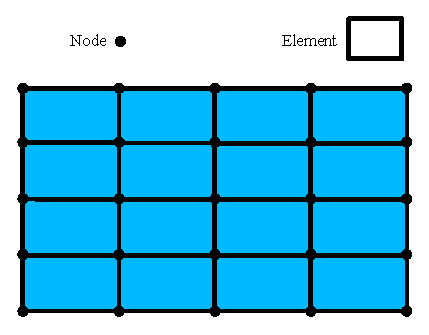
\includegraphics{FirstStepMesh}}
    \caption{Mesh of $4 \times 4$ elements on a rectangular domain. Here
    each element is a quadrilateral and described by four nodes, namely
    the corner points. The solution is interpolated by a bi-linear
    polynomial.}
    \label{fig:FirstSteps.2}
\end{figure}

In general the BVP\index{boundary value problem!BVP} cannot be solved
analytically and numerical methods are used to construct an
approximation of the solution $u$.
Here we will use the finite element method\index{finite element method}
(FEM\index{finite element method!FEM}).
The basic idea is to fill the domain with a set of points called nodes.
The solution is approximated by its values on the nodes\index{finite element method!nodes}.
Moreover, the domain is subdivided into smaller sub-domains called
elements\index{finite element method!element}.
On each element the solution is represented by a polynomial of a certain
degree through its values at the nodes located in the element.
The nodes and their connection through elements is called a
mesh\index{finite element method!mesh}. \fig{fig:FirstSteps.2} shows an
example of a FEM mesh with four elements in the $x_0$ and four elements
in the $x_1$ direction over the unit square.
For more details we refer the reader to the literature, for instance \Refe{Zienc,NumHand}.

The \escript solver we want to use to solve this problem is embedded into the \PYTHON interpreter language.
So you can solve the problem interactively but you will learn quickly that it
is more efficient to use scripts which can be edited with your favorite editor.
To enter the escript environment, use the \program{run-escript}
command\footnote{\program{run-escript} is not available under Windows.
If you run under Windows you can just use the \program{python} command and the
\env{OMP_NUM_THREADS} environment variable to control the number of threads.}:
\begin{verbatim}
run-escript
\end{verbatim}
which will pass you on to the \PYTHON prompt
\begin{verbatim}
Python 2.7.6 (default, Mar 22 2014, 15:40:47) 
[GCC 4.8.2] on linux2
Type "help", "copyright", "credits" or "license" for more information.
>>> 
\end{verbatim}
Here you can use all available \PYTHON commands and language features\footnote{Throughout our examples, we use the python 3 form of 
print. That is, print(1) instead of print 1.}, for instance
\begin{python}
  >>> x=2+3
  >>> print("2+3=",x)
  2+3= 5
\end{python}
We refer to the \PYTHON user's guide if you are not familiar with \PYTHON.

\escript provides the class \Poisson to define a Poisson equation\index{Poisson equation}.
(We will discuss a more general form of a PDE\index{partial differential equation!PDE} 
that can be defined through the \LinearPDE class later.)
The instantiation of a \Poisson class object requires the specification of the domain $\Omega$.
In \escript \Domain class objects are used to describe the geometry of a
domain but it also contains information about the discretization methods and
the solver used to solve the PDE.
Here we use the FEM\index{finite element method} library \finley.
The following statements create the \Domain object \var{mydomain} from the 
\finley function \method{Rectangle}:
\begin{python}
  from esys.finley import Rectangle
  mydomain = Rectangle(l0=1.,l1=1.,n0=40, n1=20)
\end{python}
In this case the domain is a rectangle with the lower left corner at point $(0,0)$
and the upper right corner at $(\var{l0},\var{l1})=(1,1)$.
The arguments \var{n0} and \var{n1} define the number of elements in $x_{0}$ and
$x_{1}$-direction respectively. For more details on \method{Rectangle} and
other \Domain generators see \Chap{chap:finley}, \Chap{chap:ripley}, and
\Chap{chap:speckley}.

The following statements define the \Poisson class object \var{mypde} with domain \var{mydomain} and
the right hand side $f$ of the PDE to constant $1$: 
\begin{python}
  from esys.escript.linearPDEs import Poisson
  mypde = Poisson(mydomain)
  mypde.setValue(f=1)
\end{python}
We have not specified any boundary condition but the \Poisson class implicitly
assumes homogeneous Neuman boundary conditions\index{Neumann boundary condition!homogeneous} defined by \eqn{eq:FirstSteps.2}.
With this boundary condition the BVP\index{boundary value problem!BVP} we have
defined has no unique solution.
In fact, with any solution $u$ and any constant $C$ the function $u+C$ becomes
a solution as well.
We have to add a Dirichlet boundary condition\index{Dirichlet boundary condition}.
This is done by defining a characteristic function\index{characteristic function}
which has positive values at locations $x=(x_{0},x_{1})$
where Dirichlet boundary condition is set and $0$ elsewhere.
In our case of $\Gamma^D$ defined by \eqn{eq:FirstSteps.2c}, we need to
construct a function \var{gammaD} which is positive for the cases $x_{0}=0$ or $x_{1}=0$.
To get an object \var{x} which contains the coordinates of the nodes in the domain use
\begin{python}
  x=mydomain.getX() 
\end{python}
The method \method{getX} of the \Domain \var{mydomain} gives access to locations
in the domain defined by \var{mydomain}.
The object \var{x} is actually a \Data object which will be discussed in
\Chap{ESCRIPT CHAP} in more detail.
What we need to know here is that \var{x} has \Rank (number of dimensions) and
a \Shape (list of dimensions) which can be viewed by calling the \method{getRank} and \method{getShape} methods:
\begin{python}
  print("rank ",x.getRank(),", shape ",x.getShape())
\end{python}
This will print something like
\begin{python}
  rank 1, shape (2,)
\end{python}
The \Data object also maintains type information which is represented by the 
\FunctionSpace of the object. For instance
\begin{python}
  print(x.getFunctionSpace())
\end{python}
will print 
\begin{python}
  Finley_Nodes [ContinuousFunction(domain)] on FinleyMesh 
\end{python}
which tells us that the coordinates are stored on the nodes of (rather than on
points in the interior of) a Finley mesh.
To get the  $x_{0}$ coordinates of the locations we use the statement 
\begin{python}
  x0=x[0]
\end{python}
Object \var{x0} is again a \Data object now with \Rank $0$ and \Shape $()$.
It inherits the \FunctionSpace from \var{x}:
\begin{python}
  print(x0.getRank(), x0.getShape(), x0.getFunctionSpace())
\end{python}
will print
\begin{python}
  0 () Finley_Nodes [ContinuousFunction(domain)] on FinleyMesh
\end{python}
We can now construct a function \var{gammaD} which is only non-zero on the
bottom and left edges of the domain with
\begin{python}
  from esys.escript import whereZero
  gammaD=whereZero(x[0])+whereZero(x[1])
\end{python}

\code{whereZero(x[0])} creates a function which equals $1$ where \code{x[0]} is (almost) equal to zero and $0$ elsewhere. 
Similarly, \code{whereZero(x[1])} creates a function which equals $1$ where \code{x[1]} is equal to zero and $0$ elsewhere.
The sum of the results of \code{whereZero(x[0])} and \code{whereZero(x[1])}
gives a function on the domain \var{mydomain} which is strictly positive where $x_{0}$ or $x_{1}$ is equal to zero.
Note that \var{gammaD} has the same \Rank, \Shape and \FunctionSpace as \var{x0} used to define it.
So from 
\begin{python}
  print(gammaD.getRank(), gammaD.getShape(), gammaD.getFunctionSpace())
\end{python}
one gets 
\begin{python}
  0 () Finley_Nodes [ContinuousFunction(domain)] on FinleyMesh
\end{python}
An additional parameter \var{q} of the \code{setValue} method of the \Poisson
class defines the characteristic function\index{characteristic function} of
the locations of the domain where the homogeneous Dirichlet boundary condition\index{Dirichlet boundary condition!homogeneous} is set.
The complete definition of our example is now:
\begin{python}
  from esys.escript.linearPDEs import Poisson
  x = mydomain.getX()
  gammaD = whereZero(x[0])+whereZero(x[1])
  mypde = Poisson(domain=mydomain)
  mypde.setValue(f=1,q=gammaD)
\end{python}
The first statement imports the \Poisson class definition from the \linearPDEs module.
To get the solution of the Poisson equation defined by \var{mypde} we just have to call its \method{getSolution} method. 

Now we can write the script to solve our Poisson problem
\begin{python}
  from esys.escript import *
  from esys.escript.linearPDEs import Poisson
  from esys.finley import Rectangle
  # generate domain:
  mydomain = Rectangle(l0=1.,l1=1.,n0=40, n1=20)
  # define characteristic function of Gamma^D
  x = mydomain.getX()
  gammaD = whereZero(x[0])+whereZero(x[1])
  # define PDE and get its solution u
  mypde = Poisson(domain=mydomain)
  mypde.setValue(f=1, q=gammaD)
  u = mypde.getSolution()
\end{python}
The question is what we do with the calculated solution \var{u}.
Besides postprocessing, e.g. calculating the gradient or the average value,
which will be discussed later, plotting the solution is one of the things you
might want to do.
\escript offers two ways to do this, both based on external modules or packages.
The first option uses the \MATPLOTLIB module which allows plotting of 2D
results relatively quickly from within the \PYTHON script, see~\cite{matplotlib}.
However, there are limitations when using this tool, especially for large
problems and when solving three-dimensional problems.
Therefore, \escript provides functionality to export data as files which can
subsequently be read by third-party software packages such as
\mayavi\cite{mayavi} or \VisIt~\cite{VisIt}.

\subsection{Plotting Using \MATPLOTLIB}
The \MATPLOTLIB module provides a simple and easy-to-use way to visualize PDE
solutions (or other \Data objects).
To hand over data from \escript to \MATPLOTLIB the values need to be mapped onto
a rectangular grid. We will make use of the \numpy module for this.

First we need to create a rectangular grid which is accomplished by the following statements:
\begin{python}
  import numpy
  x_grid = numpy.linspace(0., 1., 50)
  y_grid = numpy.linspace(0., 1., 50)
\end{python}
\var{x_grid} is an array defining the x coordinates of the grid while
\var{y_grid} defines the y coordinates of the grid.
In this case we use $50$ points over the interval $[0,1]$ in both directions. 

Now the values created by \escript need to be interpolated to this grid.
We will use the \SCIPY \function{interpolate.griddata} function to do this.
Spatial coordinates are easily extracted as a \var{list} by
\begin{python}
  x=mydomain.getX()[0].toListOfTuples()
  y=mydomain.getX()[1].toListOfTuples()
\end{python}
In principle we can apply the same \member{toListOfTuples} method to extract the values from the PDE solution \var{u}.
However, we have to make sure that the \Data object we extract the values from
uses the same \FunctionSpace as we have used when extracting \var{x} and \var{y}.
We apply the \function{interpolation} to \var{u} before extraction to achieve this:
\begin{python}
  z=interpolate(u, mydomain.getX().getFunctionSpace())
\end{python}
The values in \var{z} are the values at the points with the coordinates given by \var{x} and \var{y}.
These values are interpolated to the grid defined by \var{x_grid} and \var{y_grid} by using
\begin{python}
   import scipy.interpolate
   z_grid = scipy.interpolate.griddata((x,y),z,(x_grid[None,:],y_grid[:,None]),'linear')
\end{python}
Now \var{z_grid} gives the values of the PDE solution \var{u} at the grid which can be plotted using \function{contourf}:
\begin{python}
  import matplotlib
  matplotlib.pyplot.contourf(x_grid, y_grid, z_grid, 5)
  matplotlib.pyplot.savefig("u.png")
\end{python}
Here we use 5 contours. The last statement writes the plot to the file \file{u.png} in the PNG format.
Alternatively, one can use 
\begin{python}
  matplotlib.pyplot.contourf(x_grid, y_grid, z_grid, 5)
  matplotlib.pyplot.show()
\end{python}
which gives an interactive browser window.

\begin{figure}
\centerline{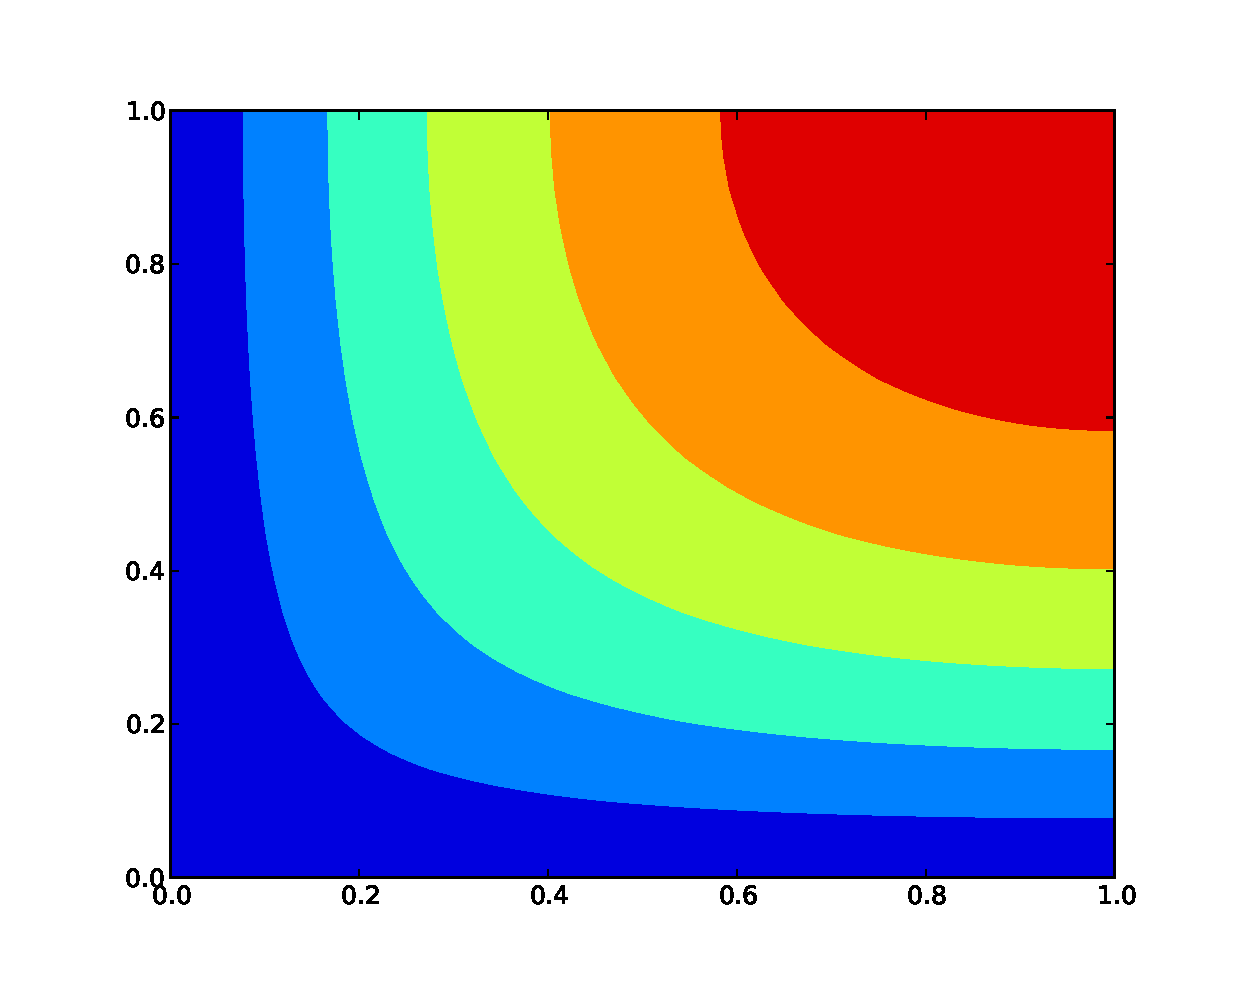
\includegraphics[width=\figwidth]{FirstStepResultMATPLOTLIB}}
\caption{Visualization of the Poisson Equation Solution for $f=1$ using \MATPLOTLIB}
\label{fig:FirstSteps.3b}
\end{figure}

Now we can write the script to solve our Poisson problem
\begin{python}
  from esys.escript import *
  from esys.escript.linearPDEs import Poisson
  from esys.finley import Rectangle
  import scipy.interpolate
  import numpy
  import matplotlib

  import pylab
  # generate domain:
  mydomain = Rectangle(l0=1.,l1=1.,n0=40, n1=20)
  # define characteristic function of Gamma^D
  x = mydomain.getX()
  gammaD = whereZero(x[0])+whereZero(x[1])
  # define PDE and get its solution u
  mypde = Poisson(domain=mydomain)
  mypde.setValue(f=1,q=gammaD)
  u = mypde.getSolution()
  # interpolate u to a matplotlib grid:
  x_grid = numpy.linspace(0.,1.,50)
  y_grid = numpy.linspace(0.,1.,50)
  x=mydomain.getX()[0].toListOfTuples()
  y=mydomain.getX()[1].toListOfTuples()
  z=interpolate(u,mydomain.getX().getFunctionSpace()).toListOfTuples()
  z_grid = scipy.interpolate.griddata((x,y),z,(x_grid[None,:],y_grid[:,None]),'linear')
  # interpolate u to a rectangular grid:
  matplotlib.pyplot.contourf(x_grid, y_grid, z_grid, 5)
  matplotlib.pyplot.savefig("u.png")
\end{python}
The entire code is available as \file{poisson_matplotlib.py} in the \ExampleDirectory.
You can run the script using the {\it escript} environment
\begin{verbatim}
run-escript poisson_matplotlib.py
\end{verbatim}
This will create a file called \file{u.png}, see \fig{fig:FirstSteps.3b}.
For details on the usage of the \MATPLOTLIB module we refer to the documentation~\cite{matplotlib}.

As pointed out, \MATPLOTLIB is restricted to the two-dimensional case and
should be used for small problems only.
It can not be used under \MPI as the \member{toListOfTuples} method is not
safe under \MPI\footnote{The phrase 'safe under \MPI' means that a program
will produce correct results when run on more than one processor under \MPI.}.

\begin{figure}
\centerline{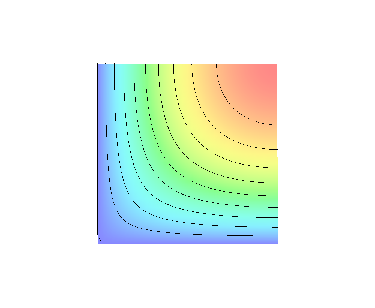
\includegraphics[width=\figwidth]{FirstStepResult}}
\caption{Visualization of the Poisson Equation Solution for $f=1$}
\label{fig:FirstSteps.3}
\end{figure}

\subsection{Visualization using export files}

As an alternative to \MATPLOTLIB, {\it escript} supports exporting data to
\VTK and \SILO files which can be read by visualization tools such as
\mayavi\cite{mayavi} and \VisIt~\cite{VisIt}. This method is \MPI safe and
works with large 2D and 3D problems.

To write the solution \var{u} of the Poisson problem in the \VTK file format
to the file \file{u.vtu} one needs to add:
\begin{python}
  from esys.weipa import saveVTK
  saveVTK("u.vtu", sol=u)
\end{python}
This file can then be opened in a \VTK compatible visualization tool where the
solution is accessible by the name {\it sol}. Similarly,
\begin{python}
  from esys.weipa import saveSilo
  saveSilo("u.silo", sol=u)
\end{python}
will write \var{u} to a \SILO file if escript was compiled with support for
LLNL's \SILO library.

The Poisson problem script is now 
\begin{python}
  from esys.escript import *
  from esys.escript.linearPDEs import Poisson
  from esys.finley import Rectangle
  from esys.weipa import saveVTK
  # generate domain:
  mydomain = Rectangle(l0=1.,l1=1.,n0=40, n1=20)
  # define characteristic function of Gamma^D
  x = mydomain.getX()
  gammaD = whereZero(x[0])+whereZero(x[1])
  # define PDE and get its solution u
  mypde = Poisson(domain=mydomain)
  mypde.setValue(f=1,q=gammaD)
  u = mypde.getSolution()
  # write u to an external file
  saveVTK("u.vtu",sol=u)
\end{python}
The entire code is available as \file{poisson_vtk.py} in the \ExampleDirectory.

You can run the script using the {\it escript} environment and visualize the
solution using \mayavi:
\begin{verbatim}
run-escript poisson_vtk.py
mayavi2 -d u.vtu -m Surface
\end{verbatim}
The result is shown in \fig{fig:FirstSteps.3}.


% $Id$
\chapter{How to Solve The Diffusion Equation}
\label{DIFFUSION CHAP}

\begin{figure}
\centerline{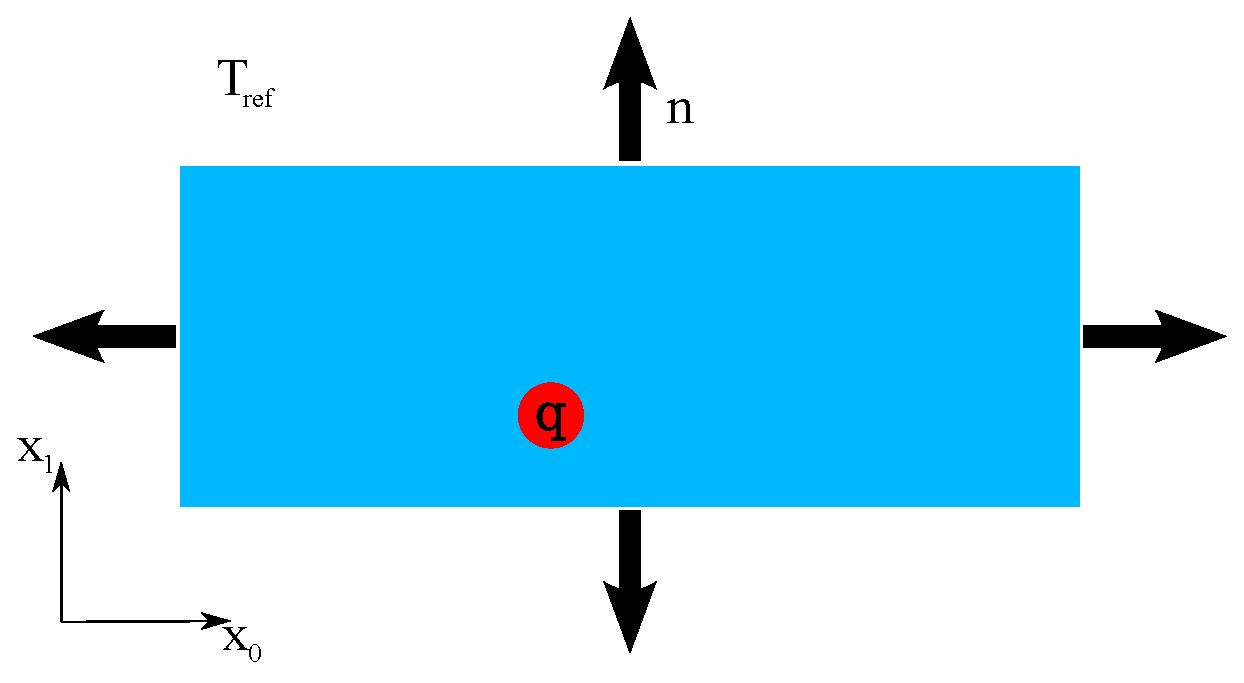
\includegraphics[width=\figwidth]{DiffusionDomain}}
\caption{Temperature Diffusion Problem with Circular Heat Source}
\label{DIFFUSION FIG 1}
\end{figure}

\begin{figure}
\centerline{
\includegraphics[width=\figwidth]{DiffusionRes1}}
\centerline{
\includegraphics[width=\figwidth]{DiffusionRes16}}
\centerline{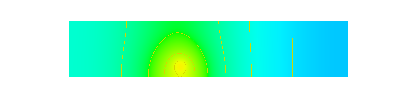
\includegraphics[width=\figwidth]{DiffusionRes32}}
\centerline{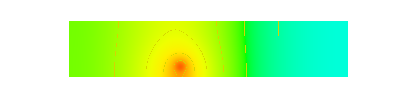
\includegraphics[width=\figwidth]{DiffusionRes48}}
\caption{Results of the Temperture Diffusion Problem for Time Steps $1$ $16$, $32$ and $48$.}
\label{DIFFUSION FIG 2}
\end{figure}


\section{\label{DIFFUSION OUT SEC}Outline}
In this chapter we will discuss how to solve the time depeneded-temperature diffusion\index{diffusion equation} within
a block of material. Within the block there is a heat source which drives the temperature diffusion.
On the surface energy can radiate into the surrounding environment.
\fig{DIFFUSION FIG 1} shows the configuration.

In the next \Sec{DIFFUSION TEMP SEC} we will present the relevant model. A 
time integration scheme is introduced to calculate the temperature at given time nodes $t^{(n)}$. 
We will see that at time step a so-called Helmholtz equation \index{Helmholtz equation} has to be solved. 
The implementation iof a Helmholtz equation solver will be discussed in \Sec{DIFFUSION HELM SEC}. 
In Section~\ref{DIFFUSION TRANS SEC} the solver of the Helmholtz equation is used to build a
solver for the temperature diffusion problem. 

\section{\label{DIFFUSION TEMP SEC}Temperature Diffusion}

The temperature $T$ is a function of its location in the domain and time $t>0$. The governing equation
in the interior of the domain is given by
\begin{equation}
\rho c\hackscore p T\hackscore{,t} - (\kappa T\hackscore{,i})\hackscore{,i} = q
\label{DIFFUSION TEMP EQ 1}
\end{equation}
where $\rho c\hackscore p$ and $\kappa$ are given material constants. In case of a composite
material the parameters are depending on the their location in the domain. $q$ is
a heat source (or sink) within the domain. We are using Einstein summation convention \index{summation convention} 
as introduced in \Chap{FirstSteps}. In our case we assume $q$ to be equal to a constant $q^{c}$
on a circle or sphere with center $x^c$ and radius $r$ and $0$ elsewhere:
\begin{equation}
q(x,t)=
\left\{ 
\begin{array}{lcl}
q^c  & & \|x-x^c\| \le r \\
     & \mbox{if} \\
0    &  & \mbox{else} \\
\end{array}
\right.
\label{DIFFUSION TEMP EQ 1b}
\end{equation}
for all $x$ in the domain and all time  $t>0$.

On the surface of the domain we are 
are specifying a radiation condition 
which precribes the normal component of the flux $J\hackscore i= \kappa T\hackscore{,i}$ to be proportional
to the difference of the current temperature to the surrounding temperature $T\hackscore{ref}$:    
\begin{equation}
 \kappa T\hackscore{,i} n\hackscore i = \eta (T\hackscore{ref}-T) 
\label{DIFFUSION TEMP EQ 2}
\end{equation}
$\eta$ is a given material coefficient depending on the material and the surrounding medium. 
As usual $n_i$ is the $i$-th component of the outer normal field \index{outer normal field}
at the surface of the domain. 

To solve the the time depended \eqn{DIFFUSION TEMP EQ 1} the initial temperature at time 
$t=0$ has to be given. Here we assume that the initial temperature is the surrounding temperature:
\begin{equation}
T(x,0)=T\hackscore{ref} 
\label{DIFFUSION TEMP EQ 4}
\end{equation}
for all $x$ in the domain. It is pointed out that 
the initial conditions is fullfilling the 
boundary condition defined by \eqn{DIFFUSION TEMP EQ 2}. 

The temperature is calculated discrete time nodes $t^{(n)}$ where 
$t^{(0)}=0$ and  $t^{(n)}=t^{(n-1)}+h$ where $h>0$ is the step size which is assumed to be constant. 
In the following the upper index ${(n)}$ is refering to a value at time $t^{(n)}$. The simplest
and most robust scheme to approximate the time derivative of the the temperature is the 
\index{backward Euler} scheme, see~\cite{XXX} for alternatives. The backward Euler scheme bases
on the Taylor expansion
\begin{equation}
T^{(n-1)}\approx T^{(n)}+T\hackscore{,t}^{(n)}(t^{(n-1)}-t^{(n)})
=T^{(n-1)} + h \cdot T\hackscore{,t}^{(n)}
\label{DIFFUSION TEMP EQ 6}
\end{equation}
which is inserted into \eqn{DIFFUSION TEMP EQ 1}. By separating the terms at 
$t^{(n)}$ and  $t^{(n-1)}$ one gets for $n=1,2,3\ldots$
\begin{equation}
\frac{\rho c\hackscore p}{h} T^{(n)} - (\kappa T^{(n)}\hackscore{,i})\hackscore{,i} = q +  \frac{\rho c\hackscore p}{h} T^{(n-1)}
\label{DIFFUSION TEMP EQ 7}
\end{equation}
where $T^{(0)}=T\hackscore{ref}$ is taken form the initial condition given by \eqn{DIFFUSION TEMP EQ 4}.
Together with the natural boundary condition from \eqn{DIFFUSION TEMP EQ 2}.
this forms a boundary value problem that has to be solved for each time step. 
As a first step to implement a solver for the temperature diffusion problem we will 
first implement a solver for the  boundary value problem that has to be solved at each time step.

\section{\label{DIFFUSION HELM SEC}Helmholtz Problem}
The partial differential equation to be solved for $T^{(n)}$ has the form 
\begin{equation}
\omega u  - (\kappa u\hackscore{,i})\hackscore{,i} = f
\label{DIFFUSION HELM EQ 1}
\end{equation}
where $u$ plays the role of $T^{(n)}$ and we set
\begin{equation}
\omega=\frac{\rho c\hackscore p}{h} \mbox{ and } f=q+\frac{\rho c\hackscore p}{h}T^{(n-1)} \;.
\label{DIFFUSION HELM EQ 1b}
\end{equation}
With $g=\eta T\hackscore{ref}$ the radiation condition defined by \eqn{DIFFUSION TEMP EQ 2}
takes the form 
\begin{equation}
\kappa u\hackscore{,i} n\hackscore{i} =  g - \eta u\mbox{ on } \Gamma
\label{DIFFUSION HELM EQ 2}
\end{equation}
The partial differential 
\eqn{DIFFUSION HELM EQ 1} together with boundary conditions of \eqn{DIFFUSION HELM EQ 2}
is called a Helmholtz equation \index{Helmholtz equation}. 

We want to use the \LinearPDE class provided by \escript to define and solve a general linear PDE such as the 
Helmholtz equation. We have used a special case of the \LinearPDE class, namely the
\Poisson class already in \Chap{FirstSteps}. 
Here we will write our own specialized class of the \LinearPDE to solve the Helmholtz equation. 

The general form of a single PDE that can be handeled by the \LinearPDE class is 
\begin{equation}\label{EQU.FEM.1}
-(A\hackscore{jl} u\hackscore{,l})\hackscore{,j}+D u =Y \; .
\end{equation}
The general form and systems is discussed in \Sec{SEC LinearPDE}.  
$A$, $D$ and $Y$ are the known coeffecients of the PDE \index{partial differential equation!coefficients}. 
Notice that $A$ is a matrix or tensor of order 2 and $D$ and $Y$ are scalar. 
They may be constant or may depend on their 
location in the domain but must not depend on the unknown solution $u$. 
The following natural boundary conditions \index{boundary condition!natural} that
are used in the \LinearPDE class have the form
\begin{equation}\label{EQU.FEM.2}
n\hackscore{j}A\hackscore{jl} u\hackscore{,l}+du=y  \;.
\end{equation}
where, as usual, $n$ denotes the outer normal field on the surface of the domain. Notice that 
the coefficient $A$ is already used in the PDE in \eqn{EQU.FEM.1}. $d$ and $y$ are given scalar coefficients.

By inpecting the Helmholtz equation \index{Helmholtz equation} 
we can easily assign values to the coefficients in the 
general PDE of the \LinearPDE class:
\begin{equation}\label{DIFFUSION HELM EQ 3}
\begin{array}{llllll}
A\hackscore{ij}=\kappa \delta\hackscore{ij} & D=\omega & Y=f \\
d=\eta & y= g &  \\
\end{array}
\end{equation}
$\delta\hackscore{ij}$ is the Kronecker symbol \index{Kronecker symbol} defined by $\delta=\hackscore{ij}=1$ for
$i=j$ and $0$ otherwise.

We want to implement a 
new class which we will call \class{Helmholtz} that provides the same methods like the \LinearPDE class but
is defined through the coefficeints $\kappa$, $\omega$, $f$, $\eta$, 
$g$ rather than the general form given by \eqn{EQU.FEM.1}.
Python's
mechanism of inhertence allows doing this in a very easy way. 
The advantage is that our new \class{Helmholtz} can be used in any context 
that works with a \LinearPDE class but with an easier interface to define the PDE.
This improves reuasablity as well as maintainability of program codes.

We want to implement a 
new class which we will call \class{Helmholtz} that provides the same methods like the \LinearPDE class but
is defined through the coefficeints $\kappa$, $\omega$, $f$, $\alpha$, 
$g$ rather than the general form given by \eqn{EQU.FEM.1}. 
Python's mechanism of subclasses allows doing this in a very easy way.
The \Poisson class of the \linearPDEsPack module,
which we have already used in \Chap{FirstSteps}, is in fact a subclass of the 
\LinearPDE class. That means that it all methods (such as the \method{getSolution})
from the parent class \LinearPDE are defined for any \Poisson object. However, new
methods can be added and methods of the parent class can be redefined. In fact,
the \Poisson class redefines the \method{setValue} of the \LinearPDE class which is called to assign 
values to the coefficients of the PDE. This is exactly what we will do when we define 
our new \class{Helmholtz} class:
\begin{python}
from esys.linearPDEs import LinearPDE
import numarray
class Helmholtz(LinearPDE)
   def setValue(self,kappa=0,omega=1,f=0,eta=0,g=0)
        self._setValue(A=kappa*numarray.identity(self.getDim()),D=omega,Y=f,d=eta,y=g)
\end{python}
\code{class Helmholtz(linearPDE)} declares the new \class{Helmholtz} class as a subclass 
of the \LinearPDE which have imported in the first line of the script. 
We add the method \method{setValue} to the class which overwrites the 
\method{setValue} method of the \LinearPDE class. The new methods which has the 
parameters of the Helmholtz \eqn{DIFFUSION HELM EQ 1} as arguments 
maps the parameters of the coefficients of the general PDE defined 
in \eqn{EQU.FEM.1}. The coefficient \var{A} is defined by Kroneckers symbol. we use the
\numarray function \function{identity} which return a square matrix which has ones on the
main diagonal and zeros out side the main diagonal. The argument of \function{identity} gives the order of the matrix.
Here we use
the \method{getDim} of the \LinearPDE class object \var{self} to get the spatial dimension of the domain of the
PDE. As we will make use of the \class{Helmholtz} class several times, it is convient to 
put is definition into a file which we name \file{mytools.py} available in the \ExampleDirectory.
You can use your favourite editor to create and edit the file.   

An object of the \class{Helmholtz} class is created through the statments:
\begin{python}
from mytools import *
mypde=Helmholtz(mydomain)
mypde.setValue(kappa=10.,omega=0.1,f=12)
u=mypde.getSolution()
\end{python}
In the first statement we import all definition from the \file{mytools.py}  \index{scripts!\file{mytools.py}}. Make sure
that \file{mytools.py} is in directory from where you have started Python.
\var{mydomain} is the \Domain of the PDE. In the third statment values are
assigned to the PDE parameters. As no values for arguments \var{eta} and \var{g} are
specified the default values $0$ are used \footnote{It would be better to use the default value 
\var{escript.Data()} rather then $0$ as then the coefficient would be defined as being not present and
would not be processed when the PDE is evaluated.}. In the forth statement the solution of the
PDE is returned. 

We want to test our \class{Helmholtz} class on a rectangular domain
of length $l$ and height $h$. We do this by choosing a simple test solution,
here we take $u=x\hackscore{0}$ and then calculate the right hand side terms $f$ and $g$ such that
the test solution becomes the solution of the problem. If we take $\kappa=1$ 
an easy calculation shows that we have to choose $f=\omega \cdot x\hackscore{0}$. On the boundary we get
$\kappa n\hackscore{i} u\hackscore{,i}=n\hackscore{0}$.  
So we have to set $g=n\hackscore{0}+\eta x\hackscore{0}$. The following script \file{helmholtztest.py} 
\index{scripts!\file{helmholtztest.py}} which is available in the \ExampleDirectory
implements this test problem using the \finley PDE solver:
\begin{python}
from mytools import *
from esys.escript import *
import esys.finley
#... set some parameters ...
omega=0.1
eta=10.
#... generate domain ...
mydomain = esys.finley.Rectangle(l0=5.,l1=1.,n0=50, n1=10)
#... open PDE and set coefficients ...
mypde=Helmholtz(mydomain)
n=mydomain.getNormal()
x=mydomain.getX()
mypde.setValue(1,omega,omega*x[0],eta,n[0]+eta*x[0])
#... calculate error of the PDE solution ...
u=mypde.getSolution()
print "error is ",Lsup(u-x[0])
\end{python}
The script is similar to the script \file{mypoisson.py} dicussed in \Chap{FirstSteps}.
\code{mydomain.getNormal()} returns the outer normal field on the surface of the domain. The function \function{Lsup}
is imported by the \code{from escript import *} statement and returns the maximum absulute value of it argument. To run 
The error shown by the print statement should be in the order of $10^{-7}$. As piecewise linear interpolation is
used to approximate the solution and our solution is a linear function of the spatial coordinates one may 
expect that the error is zero. However, as most PDE packages uses an iterative solver which is terminated
when a given tolerance has been reached. The default tolerance is $10^{-8}$. Thsi value can be altered by using the 
\method{setTolerance} of the \LinearPDE class. 

\section{The Transition Problem}
\label{DIFFUSION TRANS SEC}
Now we are ready to solve the original time dependent problem. The main 
part of the script is the loop over the time $t$ which takes the following form:
\begin{python}
mypde=Helmholtz(mydomain)
while t<t_end:
      mypde.setValue(kappa,rhocp/h,q+rhocp/h*T,eta,eta*Tref)
      T=mypde.getSolution()
      t+=h
\end{python}
\var{kappa}, \var{rhocp}, \var{eta} and \var{Tref} are input parameters of the model. \var{q} is the heat source
in the domain and \var{h} is the time step size which has to be chosen. Notice that the \class{Hemholtz}
is created before the loop over time is entered while in each time step only the coefficients
are reset in each time step. This way some information about the reperesentation of the PDE can be reused 
\footnote{The efficience can be improved further by setting the coefficients in the operator
\var{kappa}, \var{omega} and \var{eta} before entering the \code{while}-loop and only update the coefficients
in the right hand side \var{f} and \var{g}. This needs a more careful implementation of the \method{setValue}
method but gives the advantage that the \LinearPDE class can save rebuilding the PDE operator}. The variable \var{T}
holds the current temperature. It is used to calculate the right hand side coefficient \var{f} in the
Helmholtz \eqn{DIFFUSION HELM EQ 1}. Statement \code{T=mypde.getSolution()} overwrites \var{T} with the 
temperature of the new time step $\var{t}+\var{h}$. To get this iterative process going we need to sepcify the
initial temperature distribution, which equal to $T\hackscore{ref}$.

The heat source \var{q} which is defined in \eqn{DIFFUSION TEMP EQ 1b} shall be \var{q0}
at an area defined as a circle of radius \var{r} and center \var{xc} and zero outside this circle.
\var{q0} is a fixed constant. The following script defines \var{q} as desired:  
\begin{python}
xc=[0.02,0.002]
r=0.001
x=mydomain.getX()
q=q0*(length(x-xc)-r).whereNegative()
\end{python}
\var{x} is a \Data class object of
the \escript module defining the locations of points in the \Domain \var{mydomain}. 
\code{length(x-xc)} calculates the distances in the Euclidean norm 
of the locations \var{x} to the center of the circle \var{xc} where the heat source is acting.
Notice that the coordinates of \var{xc} are defined as a list of floating point numbers. It is independently
converted into a \Data class object before subtracted from \var{x}. The method \method{whereNegative} of
a \Data class object, in this case the result of the expression 
\code{length(x-xc)-r}, returns a \Data class which is equal one where the object negative and
zero elsewhere. After multiplication with \var{q0} we get a function with the deired property.

Now we can put the components together to the script \file{diffusion.py} which is available in the \ExampleDirectory:
\index{scripts!\file{diffusion.py}}:
\begin{python}
from mytools import *
from esys.escript import *
import esys.finley
#... set some parameters ...
x_c=[0.02,0.002]
r=0.001
q0=50.e6
Tref=0.
rhocp=2.6e6
eta=75.
kappa=240.
t_end=5.
# ...time step size and counter ...
h=0.1
i=0
t=0
#... generate domain ...
mydomain = esys.finley.Rectangle(l0=0.05,l1=0.01,n0=250, n1=50)
#... open PDE ...
mypde=Helmholtz(mydomain)
# ... set heat source: ....
x=mydomain.getX()
q=q0*(length(x-x_c)-r).whereNegative()
# ... set initial temperature ....
T=Tref
# ... start iteration:
while t<t_end:
      i+=1
      t+=h
      print "time step :",t
      mypde.setValue(kappa=kappa,omega=rhocp/h,f=q+rhocp/h*T,eta=eta,g=eta*Tref)
      T=mypde.getSolution()
      T.saveDX("T%d.dx"%i)
\end{python}
The script will create the files \file{T.1.dx},
 \file{T.2.dx}, $\ldots$, \file{T.50.dx} in the directory where the script has been started. The files give the 
temperature distributions at time steps $1$, $2$, $\ldots$, $50$ in the \OpenDX file format. 
An easy way to visualize the results is the command
\begin{verbatim}
dx -edit diffusion.net
\end{verbatim}
where \file{diffusion.net} is an \OpenDX script available in the \ExampleDirectory. 
\fig{DIFFUSION FIG 2} shows the result for some selected time steps.


% \input{wavepropagation}

% $Id$

\chapter{The module \escript}

\declaremodule{extension}{escript} \modulesynopsis{Handling data on
data points like \class{Nodes}, \class{Elements}}

The class \Data of the module \escript allows handling
data which are hold on data points \index{data points}. Examples for
data points are nodes or the quadrature points in elements of a finite
element mesh. Another examples a particles or the connection between
particles in the case of discrete element methods.  Handlers to data
points are issued by the structure which contains the data points,
e.g. a \finley mesh.

The simplest form of data attached to a data point is a single scalar
$a$ value which for instance represent the temperature or pressure at
this particular data point. Another example is a velocity field. in
this case each data point holds a vector $a(0),a(1),a(2)$ representing
the velocity at the particular data point. For the case that the
values are representing a stress tensor the value is a matrix of the
form
$a(0,0),a(0,1),a(0,2),a(1,0),a(1,1),a(1,2),a(2,0),a(2,1),a(2,2)$. In
general, values hald by data points can have up to four indices. The
number of indices is called rank \index{rank}. The tuple of length
rank which defines the upper-bound for each index component is called
the shape. A stress has rank 2 and the shape is (3,3). For a vector we
have rank 1 and shape (3,). A scalar can have rank 0 or rank 1 with
shape (1,).

In general, the data are stored for each data point. This status of
the data is called expanded \index{expanded}. But in some cases, all
data points hold the same value. In this case only a single value is
stored, which is refered by each data point if needed. This saves
memory as well as compute time. In some cases, it is very usefull to
have slightly more general way which allows to define piecewise
constant data. For this, each data point has to wear a tag which is an
integer \index{tag}. The tag is used to distingish between various
types of data points. Typical example of the usage of tags is to
assign different material parameters to various subdomains. Then one
assigns the same tag to all elements in a finite element mesh which
lay in the same subdomain.  Later each tag can be assigns individual
material parameters.

The following table shows unitary operations that can be applied to an
\Data object \var{arg}:
\begin{tableii}{l|l}{textrm}{expression}{Description}
\lineii{+\var{arg}} {just \var{arg} \index{+}}
\lineii{-\var{arg}} {swapping the sign\index{-}}
\lineii{\function{abs}(\var{arg})} {absolute value}
\lineii{\function{sin}(\var{arg})} {sine function}
\lineii{\function{cos}(\var{arg})} {cosine function}
\lineii{\function{exp}(\var{arg})} {exponential function}
\lineii{\function{sqrt}(\var{arg})} {square root}
\end{tableii}
An unitary operation returns a \Data objects of the same shape
and defined on the data points like \var{arg}.

The following table shows binary operations that can be applied to
\Data objects:
\begin{tableii}{l|l}{textrm}{expression}{Description}
\lineii{\var{arg1}+\var{arg2}} {adds \var{arg1} and \var{arg2} \index{+}}
\lineii{\var{arg1}*\var{arg2}} {multiplies \var{arg1} and \var{arg2} \index{*}}
\lineii{\var{arg1}-\var{arg2}} {difference \var{arg2} from\var{arg2} \index{-}}
\lineii{\var{arg1}/\var{arg2}} {ratio \var{arg1} by \var{arg2} \index{/}}
\lineii{\var{arg1}**\var{arg2}} {raises \var{arg1} to the power of \var{arg2} \index{**}}
\end{tableii}
At least on of the arguments \var{arg1} or \var{arg2} must be a
\Data object. One of the arguments may be an object that can be
converted into a \Data object. If \var{arg1} or \var{arg2} are
defined on different data points it is tried to interpolate \var{arg1}
onto the data points of \var{arg2} or to interpolate \var{arg2} onto
the data points of \var{arg1}. Boths arguments must have the same
shape or one of the arguments my be of rank 0 or shape (1,). In the
latter case it is assumed that the particular argument is of the same
shape like the other argument but constant over all components.

The returned \Data object has the same shape and is defined on
the data points like \var{arg1} or \var{arg2}.

The following table shows the update operations that can be applied to
\Data objects:
\begin{tableii}{l|l}{textrm}{expression}{Description}
\lineii{\var{arg1}+=\var{arg2}} {adds \var{arg1} to \var{arg2} \index{+}}
\lineii{\var{arg1}*=\var{arg2}} {multiplies \var{arg1} with \var{arg2} \index{*}}
\lineii{\var{arg1}-=\var{arg2}} {subtracts \var{arg2} from\var{arg2} \index{-}}
\lineii{\var{arg1}/=\var{arg2}} {divides \var{arg1} by \var{arg2} \index{/}}
\end{tableii}
\var{arg1} must be a \Data object. \var{arg1} must be a
\Data object or an object that can be converted into a
\Data object. \var{arg1} must have the same shape like
\var{arg1} or has rank 0 or shape (1,).  In the latter case it is
assumed that the values of \var{arg1} are constant for all
components. \var{arg2} must be defined on the same data points like
\var{arg1} or it must be possible to interpolate \var{arg2} onto the
data points where \var{arg1} is hold.


%TODO:
Slicing \index{slicing}.

\begin{classdesc}{Data}{}
A class that holds values assigned to data points.
\end{classdesc}

\begin{classdesc}{Scalar}{value=None,where=None,expand=None}
A class that holds a single value per data point.
\end{classdesc}

\begin{classdesc}{Vector}{value=None,dim=None,where=None,expand=None}
A class that holds a vector per data point.
\end{classdesc}

\begin{classdesc}{Tensor}{value=None,dim=None,where=None,expand=None}
A class that holds a tensor order 2 (matrix) per data point.
\end{classdesc}

\begin{classdesc}{Tensor3}{value=None,dim=None,where=None,expand=None}
A class that holds a tensor order 3 per data point.
\end{classdesc}

\begin{classdesc}{Tensor4}{value=None,dim=None,where=None,expand=None}
A class that holds a tensor order 4 per data point.
\end{classdesc}

\begin{funcdesc}{abs}{arg}
returns the absulute value of \Data \var{arg}. The returned
\Data object has the same rank, shape and is defined on the
same \class{_Atom} like \var{arg}. An entries in the returned object
is the absolute value of the corresponding entry in \var{arg}.
\index{absolute value}
\end{funcdesc}

\begin{funcdesc}{L2}{arg}
  returns the $L^2$-norm of the \Data \var{arg} by using method
\method{arg.L2()}.  \index{$L^2$-norm}
\end{funcdesc}

\begin{funcdesc}{grad}{arg}
returns the gradient of the interpolation function of \Data
\var{arg} by using \method{arg.grad}. \index{gradient}
\end{funcdesc}

\begin{funcdesc}{integrate}{arg}
returns the integral of the interpolation function of \Data
\var{arg} by using \method{arg.integrate}. \index{integral}
\end{funcdesc}

\begin{funcdesc}{interpolate}{arg,where}
interpolates the \Data \var{arg} onto \class{_Atom} where by
using \method{arg.interpolate}. \index{interpolation}
\end{funcdesc}

\begin{funcdesc}{transpose}{arg}
returns the transpose of \var{arg} where \var{arg} has to be
\Data or \class{numarray.array}. If \var{arg} is of
\Data the method \method{arg.transpose} is used otherwise
\function{numarray.transpose} is called. \index{transpose}
\end{funcdesc}

\begin{funcdesc}{trace}{arg}
returns the trace of \var{arg} where \var{arg} has to be \Data
or \class{numarray.array} of rank 2. If \var{arg} is of \Data
the method \method{arg.trace} is used otherwise
\function{numarray.trace} is called. \index{trace}
\end{funcdesc}

\begin{funcdesc}{exp}{arg}
applies the exponential function to \var{arg} where \var{arg} has to
be \Data or \class{numarray.array}. If \var{arg} is of
\Data the method \method{arg.exp} is used otherwise
\function{numarray.exp} is called. \index{exponential function}
\end{funcdesc}

\begin{funcdesc}{sqrt}{arg}
applies the square root function to \var{arg} where \var{arg} has to
be \Data or \class{numarray.array}. If \var{arg} is of
\Data the method \method{arg.sqrt} is used otherwise
\function{numarray.sqrt} is called. \index{square root}
\end{funcdesc}

\begin{funcdesc}{sin}{arg}
applies the sine function to \var{arg} where \var{arg} has to be
\Data or \class{numarray.array}. If \var{arg} is of
\Data the method \method{arg.sin} is used otherwise
\function{numarray.sin} is called. \index{sine function}
\end{funcdesc}

\begin{funcdesc}{cos}{arg}
applies the cosine function to \var{arg} where \var{arg} has to be
\Data or \class{numarray.array}. If \var{arg} is of
\Data the method \method{arg.cos} is used otherwise
\function{numarray.cos} is called. \index{cosine function}
\end{funcdesc}

\begin{funcdesc}{maxval}{arg}
returns for each data point the maximum value over all components of
\Data \var{arg} by using \method{arg.maxval}.  \index{maximum
value}
\end{funcdesc}

\begin{funcdesc}{minval}{arg}
returns for each data point the minimum value over all components of
\Data \var{arg} by using \method{arg.minval}.  \index{minimum
value}
\end{funcdesc}

\begin{funcdesc}{inf}{arg}
returns the minimum value (infimum) over all components and all data
points of \Data \var{arg} by using \method{arg.inf}.
\index{infimum}
\end{funcdesc}

\begin{funcdesc}{sup}{arg}
returns the maximum value (supremum) over all components and all data
points of \Data \var{arg} by using \method{arg.sup}.
\index{supremum}
\end{funcdesc}

\begin{funcdesc}{Lsup}{arg}
returns the maximum absulute value ($L^{sup}$-norm) over all
components and all data points of \Data \var{arg} by using
\method{arg.sup}.  The returned value equals
\function{sup}(\function(arg)).  \index{$L^{sup}$-norm}
\end{funcdesc}

\begin{funcdesc}{matmult}{arg1,arg2}
returns for each data point the matrix-matrix product of \var{arg1}
and \var{arg2} \index{matrix-matrix product}. At least of the
arguments \var{arg1} and \var{arg2} has to be a \Data
object. If the other argument is not a \Data object it must be
convertable into a \Data object. The returned \Data
object has rank \var{arg1.getRank()}+\var{arg2.getRank()}-2 and shape
(\var{arg1.getShape()}[r-1],\var{arg2.getShape()}[1:]), where
\var{r}=\var{arg1.getRank()}. The last dimension of \var{arg1} and the
first dimension of \var{arg2} have to match,
i.e. \var{arg1.getShape()[r-1]}=\var{arg2.getShape()[0]}

For the case that \var{arg1} and \var{arg2} are both of rank $2$ the
result \var{res} is calculated as
\begin{equation}
res(i,j;s)=
arg1(i,0;s) \cdot arg2(0,j;s)+
\ldots
arg1(i,n-1;s) \cdot arg2(n-1,j;s)
\end{equation}
for all $0\le i <$ \var{arg1.getShape()[0]}, $0\le j <$
\var{arg2.getShape()[1]} and all data points $s$, where
$n$=\var{arg2.getShape()[0]},

If the arguments are not defined on the same data points, \var{arg1}
is tried to be interpolated on the data points of \var{arg2} or
\var{arg2} is tried to be interpolated on the data points of
\var{arg1}. What ever case works defines the data points of the
result.
\end{funcdesc}

%==================================================================
\section{\Data class}
\begin{classdesc}{Data}{value=None,shape=None,where=None,expand=None}
\end{classdesc}

\begin{methoddesc}[Data]{getAtoms}{}
returns a handel to the data points on which the object is definded
\index{data points}.  The returned object is of \class{_Atoms}.
\end{methoddesc}

\begin{methoddesc}[Data]{getShape}{}
returns the shape of the data on each data point as a \class{tuple} of
integers. \index{shape}
\end{methoddesc}

\begin{methoddesc}[Data]{getRank}{}
returns the rank of the data on each data point. \index{rank}
\end{methoddesc}

\begin{methoddesc}[Data]{hasShape}{shape}
is true if the object has the shape \var{shape}.
\end{methoddesc}

\begin{methoddesc}[Data]{expand}{}
returns an expanded version of the object if the object is not
expanded. Otherwise it returns itself. \index{expanded}
\end{methoddesc}

\begin{methoddesc}[Data]{makeExpanded}{}
turns the object into an expanded \Data
object. \index{expanded}
\end{methoddesc}

\begin{methoddesc}[Data]{isExpanded}{}
is true if the object is expanded. \index{expanded}
\end{methoddesc}

\begin{methoddesc}[Data]{isTagged}{}
is true if the object is defined using tags. \index{tagged}
\end{methoddesc}

\begin{methoddesc}[Data]{asArray}{}
returns the object as a \class{numarray.array} array. The array is one
rank higher than the rank of the object. The extra dimension is the
number of data points.
% TODO: be more accurate on the shape
\end{methoddesc}

\begin{methoddesc}[Data]{addTaggedValue}{tag,value=0}
assigns the \var{value} to all data points which have the tag
\var{tag} which has to be an integer or a list of
integers. \var{value} must be an object of class
\class{numarray.array} or must be convertable into a
\class{numarray.array} object. \var{value} (or the cooresponding
\class{numarray.array} object) must be of rank $0$ or must have the
same rank like the object. \index{tagged}

If a value has allready be defined for tag \var{tag} within the object
it is overwritten by the new \var{value}.  If the object is expanded,
the value assigned to data points with tag \var{tag} is replaced by
\var{value}.
\end{methoddesc}

\begin{methoddesc}[Data]{getTaggedValue}{tag}
returns the value assigned to \var{tag}. An exception is raised if the
object is not defined by tagged data, e.g. if the object is
expanded.\index{tagged}
\end{methoddesc}

\begin{methoddesc}[Data]{L2}{}
returns the $L^2$-norm of the object. This is square root of sum of
the squares of all values over all components and all data points.
\index{$L^2$-norm}
\end{methoddesc}

\begin{methoddesc}[Data]{grad}{}
returns the gradient of the interpolation function. The returned
\Data object is of rank r+1 where r is the rank of the object.
Typically the object of to be defined on nodes and the returned
gradient is defined on the quadrature points of elements.
\index{gradient}
\end{methoddesc}

\begin{methoddesc}[Data]{integrate}{}
returns the integral of the interpolation function. The method returns
a \class{numarray.array} object of the same shape like the object.  A
component of the returned object is the integral of the corresponding
component of the object.  \index{integral}
\end{methoddesc}

\begin{methoddesc}[Data]{interpolate}{where}
interpolates onto the data points of the \class{_Atom}
\var{where}. The returned \Data object is of the same shape
like the object and is defined on the data points \var{where}.
\index{interpolation}
\end{methoddesc}

\begin{methoddesc}[Data]{transpose}{}
returns the transpose of the object. The return value is an object has
the same shape and is defined on the same data points like the object.
For each data point the value is set to transposed of the
corresponding value of the object by reversing the index of the data.

For the case that object \var{self} is of rank 3 the result \var{res} is
\begin{equation}
res(i,j,k;s)=self(k,j,i;s)
\end{equation}
for all 
$0\le i <$ \var{self.getShape()[2]},
$0\le j <$ \var{self.getShape()[1]},
$0\le k <$ \var{self.getShape()[0]}
and all data points $s$.
\index{transpose}
\end{methoddesc}

\begin{methoddesc}[Data]{trace}{}
returns the trace of the object of rank 2. The return value is an
object has rank 0 or shape (1,) and is defined on the same data points
like the object. For each data point the value is set to sum of the
main diagonal entries.

For the case that object \var{self} is of rank 2 the result \var{res}
is
\begin{equation}
res(0;s)=
self(0,0;s)+
self(1,1;s)+
\ldots +
self(n,n;s)
\end{equation}
for all data points $s$ where
$n=min($\var{self.getShape()[0]},\var{self.getShape()[1]}$)$.
\index{trace}
\end{methoddesc}

\begin{methoddesc}[Data]{exp}{}
applies the exponential function to the values of the object. The
return value is an object has the same shape and is defined on the
same data points like the object.  For each data point and all
components the value is calculated by applying the exponention
function to the corresponding value of the object.  \index{exponential
function}
\end{methoddesc}

\begin{methoddesc}[Data]{sqrt}{}
applies the square root function to the values of the object. The
return value is an object has the same shape and is defined on the
same data points like the object.  For each data point and all
components the value is calculated by applying the square root
function to the corresponding value of the object. An exception is
raised if the value is negative.  \index{square root}
\end{methoddesc}

\begin{methoddesc}[Data]{sin}{}
applies the sine function to the values of the object. The return
value is an object has the same shape and is defined on the same data
points like the object.  For each data point and all components the
value is calculated by applying the sine function to the
corresponding value of the object.  \index{sine function}
\end{methoddesc}

\begin{methoddesc}[Data]{cos}{}
applies the cosine function to the values of the object. The return
value is an object has the same shape and is defined on the same data
points like the object.  For each data point and all components the
value is calculated by applying the cosine function to the
corresponding value of the object.  \index{cosine function}
\end{methoddesc}

\begin{methoddesc}[Data]{maxval}{}
returns for each data point the maximum value over all components. The
return value is an object of rank 0 or shape (1,) and is defined on
the same data points like the object.  \index{maximum value}
\end{methoddesc}

\begin{methoddesc}[Data]{minval}{}
returns for each data point the minimum value over all components. The
return value is an object of rank 0 or shape (1,) and is defined on
the same data points like the object.  \index{minimum value}
\end{methoddesc}

\begin{methoddesc}[Data]{inf}{}
returns the minimum value (infimum) of the object. The minimum is
taken over all components and all data points.  \index{infimum}
\end{methoddesc}

\begin{methoddesc}[Data]{sup}{}
returns the maximum value (supremum) of the object. The maximum is
taken over all components and all data points.  \index{supremum}
\end{methoddesc}

\begin{methoddesc}[Data]{Lsup}{}
returns the $L^{sup}$-norm of the object. This is maximum value of the
absolut values of the object over all data points and all components.
\index{$L^{sup}$-norm}
\end{methoddesc}

\begin{methoddesc}[Data]{wherePositive}{}
returns \Data object which has the same shape and is defined on
the same data points like the object. The returned values are $1$
where the object is positive and $0$ elsewhere.
\end{methoddesc}

\begin{methoddesc}[Data]{whereNonnegative}{}
returns \Data object which has the same shape and is defined on
the same data points like the object. The returned values are $1$
where the object is non-negative and $0$ elsewhere.
\end{methoddesc}

\begin{methoddesc}[Data]{whereNegative}{}
returns \Data object which has the same shape and is defined on
the same data points like the object. The returned values are $1$
where the object is negative and $0$ elsewhere.
\end{methoddesc}

\begin{methoddesc}[Data]{whereZero}{tolerance=Constants.EPSILON}
returns \Data object which has the same shape and is defined on
the same data points like the object. The returned values are $1$
where the object is nearly zero, i.e. where the absolute value is less
than \var{tolerance}, and $0$ elsewhere.
\end{methoddesc}

\begin{methoddesc}[Data]{whereNonzero}{tolerance=Constants.EPSILON}
returns \Data object which has the same shape and is defined on
the same data points like the object. The returned values are $1$
where the object is nearly non-zero, i.e. where the absolute value is
greater or equal than \var{tolerance}, and $0$ elsewhere.
\end{methoddesc}

\begin{methoddesc}[Data]{saveDX}{fileName}
saves the object to an openDX format file of name \var{fileName}, see
\ulink{www.opendx.org}{\url{www.opendx.org}}.  \index{openDX}
\end{methoddesc}

\begin{methoddesc}[Data]{saveMM}{fileName}
saves the object to a matrix market format file of name
\var{fileName}, see
\ulink{maths.nist.gov/MatrixMarket}{\url{http://maths.nist.gov/MatrixMarket}}.
\index{Matrix Market}
\end{methoddesc}

%=====================================================
\section{Subclasses of \var{class}}
\begin{classdesc}{Scalar}{value=None,where=None,expand=None}
\Data object with a single value (scalar) per data
point. \var{value} must be a float number.  If \var{expand} is true,
the \var{value} is copied to each data point.
\end{classdesc}

\begin{classdesc}{Vector}{value=None,dim=None,where=None,expand=None}
\Data object with a vector of length \var{dim} value (scalar)
per data point.  If \var{dim} is not present or equals \var{None},
\var{dim} is assumed to be the spatial dimension of the data points
defined by \var{where}. \var{value} may be a float number or a
\class{numarray.array} object with shape (\var{dim},).  If
\var{expand} is true, the \var{value} is copied to each data point.
\end{classdesc}

\begin{classdesc}{Tensor}{value=None,dim=None,where=None,expand=None}
\Data object with a \var{dim} $\times$ \var{dim} - tensor of
order 2 per data point.  If \var{dim} is not present or equals
\var{None}, \var{dim} is assumed to be the spatial dimension of the
data points defined by \var{where}. \var{value} may be a float number
or a \class{numarray.array} object with shape (\var{dim},\var{dim}).
If \var{expand} is true, the \var{value} is copied to each data point.
\end{classdesc}

\begin{classdesc}{Tensor3}{value=None,dim=None,where=None,expand=None}
\Data object with a \var{dim} $\times$ \var{dim} $\times$
\var{dim} - tensor of order 3 per data point.  If \var{dim} is not
present or equals \var{None}, \var{dim} is assumed to be the spatial
dimension of the data points defined by \var{where}. \var{value} may
be a float number or a \class{numarray.array} object with shape
(\var{dim},\var{dim},var{dim}).  If \var{expand} is true, the
\var{value} is copied to each data point.
\end{classdesc}

\begin{classdesc}{Tensor4}{value=None,dim=None,where=None,expand=None}
\Data object with a \var{dim} $\times$ \var{dim} $\times$
\var{dim} $\times$ \var{dim} - tensor of order 4 per data point.  If
\var{dim} is not present or equals \var{None}, \var{dim} is assumed to
be the spatial dimension of the data points defined by
\var{where}. \var{value} may be a float number or a
\class{numarray.array} object with shape
(\var{dim},\var{dim},var{dim},var{dim}).  If \var{expand} is true, the
\var{value} is copied to each data point.
\end{classdesc}


%%%%%%%%%%%%%%%%%%%%%%%%%%%%%%%%%%%%%%%%%%%%%%%%%%%%%%%%
%
% Copyright (c) 2003-2009 by University of Queensland
% Earth Systems Science Computational Center (ESSCC)
% http://www.uq.edu.au/esscc
%
% Primary Business: Queensland, Australia
% Licensed under the Open Software License version 3.0
% http://www.opensource.org/licenses/osl-3.0.php
%
%%%%%%%%%%%%%%%%%%%%%%%%%%%%%%%%%%%%%%%%%%%%%%%%%%%%%%%%


\chapter{The Module \linearPDEs}



\section{Linear Partial Differential Equations}
\label{SEC LinearPDE}

The \LinearPDE class is used to define a general linear, steady, second order PDE
for an unknown function $u$ on a given $\Omega$ defined through a \Domain object.
In the following $\Gamma$ denotes the boundary of the domain $\Omega$. $n$ denotes
the outer normal field on $\Gamma$.

For a single PDE with a solution with a single component the linear PDE is defined in the
following form:
\begin{equation}\label{LINEARPDE.SINGLE.1}
-(A\hackscore{jl} u\hackscore{,l})\hackscore{,j}-(B\hackscore{j} u)\hackscore{,j}+C\hackscore{l} u\hackscore{,l}+D u =-X\hackscore{j,j}+Y \; .
\end{equation}
$u_{,j}$ denotes the derivative of $u$ with respect to the $j$-th spatial direction. Einstein's summation convention, ie. summation over indexes appearing twice in a term of a sum is performed, is used.
The coefficients $A$, $B$, $C$, $D$, $X$ and $Y$ have to be specified through \Data objects in the
\Function on the PDE or objects that can be converted into such \Data objects.
$A$ is a \RankTwo, $B$, $C$ and $X$ are \RankOne and $D$ and $Y$ are scalar.
The following natural
boundary conditions are considered \index{boundary condition!natural} on $\Gamma$:
\begin{equation}\label{LINEARPDE.SINGLE.2}
n\hackscore{j}(A\hackscore{jl} u\hackscore{,l}+B\hackscore{j} u)+d u=n\hackscore{j}X\hackscore{j} + y  \;.
\end{equation}
Notice that the coefficients $A$, $B$ and $X$ are defined in the PDE. The coefficients $d$ and $y$ are
each a \Scalar in the \FunctionOnBoundary.  Constraints \index{constraint} for the solution prescribing the value of the
solution at certain locations in the domain. They have the form
\begin{equation}\label{LINEARPDE.SINGLE.3}
u=r \mbox{ where } q>0
\end{equation}
$r$ and $q$ are each \Scalar where $q$ is the characteristic function
\index{characteristic function} defining where the constraint is applied.
The constraints defined by \eqn{LINEARPDE.SINGLE.3} override any other condition set by \eqn{LINEARPDE.SINGLE.1}
or \eqn{LINEARPDE.SINGLE.2}.

For a system of PDEs and a solution with several components the PDE has the form
\begin{equation}\label{LINEARPDE.SYSTEM.1}
-(A\hackscore{ijkl} u\hackscore{k,l})\hackscore{,j}-(B\hackscore{ijk} u\hackscore{k})\hackscore{,j}+C\hackscore{ikl} u\hackscore{k,l}+D\hackscore{ik} u\hackscore{k} =-X\hackscore{ij,j}+Y\hackscore{i} \; .
\end{equation}
$A$ is a \RankFour, $B$ and $C$ are each a \RankThree, $D$ and $X$ are each a \RankTwo and $Y$ is a \RankOne.
The natural boundary conditions \index{boundary condition!natural} take the form:
\begin{equation}\label{LINEARPDE.SYSTEM.2}
n\hackscore{j}(A\hackscore{ijkl} u\hackscore{k,l}+B\hackscore{ijk} u\hackscore{k})+d\hackscore{ik} u\hackscore{k}=n\hackscore{j}X\hackscore{ij}+y\hackscore{i}  \;.
\end{equation}
The coefficient $d$ is a \RankTwo and $y$ is a
\RankOne both in the \FunctionOnBoundary. Constraints \index{constraint} take the form
\begin{equation}\label{LINEARPDE.SYSTEM.3}
u\hackscore{i}=r\hackscore{i} \mbox{ where } q\hackscore{i}>0
\end{equation}
$r$ and $q$ are each \RankOne. Notice that not necessarily all components must
have a constraint at all locations.

\LinearPDE also supports solution discontinuities \index{discontinuity} over contact region $\Gamma^{contact}$
in the domain $\Omega$. To specify the conditions across the discontinuity we are using the
generalised flux $J$\footnote{In some applications the definition of flux used here can be different from the commonly used definition. For instance, if $T$ is a temperature field the heat flux $q$ is defined as $q\hackscore{,i}=-\kappa T\hackscore{,i}$ ($\kappa$ is diffusifity) which differs from the definition used here by the sign. This needs to be kept in mind when defining natural boundary conditions.\index{boundary condition!natural}} which is in the case of a systems of PDEs and several components of the solution
defined as
\begin{equation}\label{LINEARPDE.SYSTEM.5}
J\hackscore{ij}=A\hackscore{ijkl}u\hackscore{k,l}+B\hackscore{ijk}u\hackscore{k}-X\hackscore{ij}
\end{equation}
For the case of single solution component and single PDE $J$ is defined
\begin{equation}\label{LINEARPDE.SINGLE.5}
J\hackscore{j}=A\hackscore{jl}u\hackscore{,l}+B\hackscore{j}u\hackscore{k}-X\hackscore{j}
\end{equation}
In the context of discontinuities \index{discontinuity} $n$ denotes the normal on the
discontinuity pointing from side 0 towards side 1. For a system of PDEs
the contact condition takes the form
\begin{equation}\label{LINEARPDE.SYSTEM.6}
n\hackscore{j} J^{0}\hackscore{ij}=n\hackscore{j} J^{1}\hackscore{ij}=y^{contact}\hackscore{i} - d^{contact}\hackscore{ik} [u]\hackscore{k} \; .
\end{equation}
where $J^{0}$ and $J^{1}$ are the fluxes on side $0$ and side $1$ of the
discontinuity $\Gamma^{contact}$, respectively. $[u]$, which is the difference
of the solution at side 1 and at side 0, denotes the jump of $u$ across $\Gamma^{contact}$.
The coefficient $d^{contact}$ is a \RankTwo and $y^{contact}$ is a
\RankOne both in the \FunctionOnContactZero or \FunctionOnContactOne.
In case of a single PDE and a single component solution the contact condition takes the form
\begin{equation}\label{LINEARPDE.SINGLE.6}
n\hackscore{j} J^{0}\hackscore{j}=n\hackscore{j} J^{1}\hackscore{j}=y^{contact} - d^{contact}[u]
\end{equation}
In this case the the coefficient $d^{contact}$ and $y^{contact}$ are each \Scalar
both in the \FunctionOnContactZero or \FunctionOnContactOne.

The PDE is symmetrical \index{symmetrical} if
\begin{equation}\label{LINEARPDE.SINGLE.4}
A\hackscore{jl}=A\hackscore{lj} \mbox{ and } B\hackscore{j}=C\hackscore{j}
\end{equation}
The system of PDEs is symmetrical \index{symmetrical} if
\begin{eqnarray}
\label{LINEARPDE.SYSTEM.4}
A\hackscore{ijkl}&=&A\hackscore{klij} \\
B\hackscore{ijk}&=&C\hackscore{kij} \\
D\hackscore{ik}&=&D\hackscore{ki} \\
d\hackscore{ik}&=&d\hackscore{ki} \\
d^{contact}\hackscore{ik}&=&d^{contact}\hackscore{ki}
\end{eqnarray}
Note that in contrast with the scalar case~\eqn{LINEARPDE.SINGLE.4} now the coefficients $D$, $d$ abd $d^{contact}$
have to be inspected.

The following example illustrates the typical usage of the \LinearPDE class:
\begin{python}
from esys.escript import *
from esys.escript.linearPDEs import LinearPDE
from esys.finley import Rectangle
mydomain = Rectangle(l0=1.,l1=1.,n0=40, n1=20)
mypde=LinearPDE(mydomain)
mypde.setSymmetryOn()
mypde.setValue(A=kappa*kronecker(mydomain),D=1,Y=1)
u=mypde.getSolution()
\end{python}
We refer to chapter~\ref{CHAP: Tutorial} for more details.

An instance of the \SolverOptions class is attached to the \LinearPDE class object. It is used to set options of the solver used to solve the PDE. In the following
code the \method{getSolverOptions} is used to access the  \SolverOptions 
attached to \var{mypde}:
\begin{python}
from esys.escript import *
from esys.escript.linearPDEs import LinearPDE, SolverOptions
from esys.finley import Rectangle
mydomain = Rectangle(l0=1.,l1=1.,n0=40, n1=20)
mypde=LinearPDE(mydomain)
mypde.setValue(A=kappa*kronecker(mydomain),D=1,Y=1)
mypde.getSolverOptions().setVerbosityOn()
mypde.getSolverOptions().setSolverMethod(SolverOptions.PCG)
mypde.getSolverOptions().setPreconditioner(SolverOptions.AMG)
mypde.getSolverOptions().setTolerance(1e-8)
mypde.getSolverOptions().setIterMax(1000)
u=mypde.getSolution()
\end{python}
In this code the preconditoned conjugate gradient method \PCG
with preconditioner \AMG. The relative tolerance is set tto $10^{-8}$ and
the maximum number of iteration steps to $1000$.

Moreover, after a completed solution call
the attached  \SolverOptions object gives access to diagnostic informations: 
\begin{python}
u=mypde.getSolution()
print 'Number of iteration steps =', mypde.getDiagnostics('num_iter')
print 'Total solution time =', mypde.getDiagnostics('time')
print 'Set-up time =', mypde.getDiagnostics('set_up_time')
print 'Net time =', mypde.getDiagnostics('net_time')
print 'Residual norm of returned solution =', mypde.getDiagnostics('residual_norm')
\end{python}
Typically a negative value for a diagnostic value indicates that the value is undefined.

\subsection{Classes}
\declaremodule{extension}{esys.escript.linearPDEs} 
\modulesynopsis{Linear partial differential equation handler}
The module \linearPDEs provides an interface to define and solve linear partial
differential equations within \escript. The module \linearPDEs does not provide any
solver capabilities in itself but hands the PDE over to
the PDE solver library defined through the \Domain of the PDE, eg. \finley.
The general interface is provided through the \LinearPDE class. The \Poisson
class which is also derived form the \LinearPDE class should be used
to define the Poisson equation \index{Poisson}.

\subsection{\LinearPDE class}
This is the general class to define a linear PDE in \escript. We list a selection of the most
important methods of the class. For a complete list, see the reference at \ReferenceGuide.

\begin{classdesc}{LinearPDE}{domain,numEquations=0,numSolutions=0}
opens a linear, steady, second order PDE on the \Domain \var{domain}. \var{numEquations}
and \var{numSolutions} gives the number of equations and the number of solution components.
If \var{numEquations} and \var{numSolutions} is non-positive, the number of equations
and the number solutions, respectively, stay undefined until a coefficient is
defined.
\end{classdesc}

\subsubsection{\LinearPDE methods}

\begin{methoddesc}[LinearPDE]{setValue}{
\optional{A}\optional{, B},
\optional{, C}\optional{, D}
\optional{, X}\optional{, Y}
\optional{, d}\optional{, y}
\optional{, d_contact}\optional{, y_contact}
\optional{, q}\optional{, r}}
assigns new values to coefficients. By default all values are assumed to be zero\footnote{
In fact it is assumed they are not present by assigning the value \code{escript.Data()}. The
can by used by the solver library to reduce computational costs.
}
If the new coefficient value is not a \Data object, it is converted into a \Data object in the
appropriate \FunctionSpace.
\end{methoddesc}

\begin{methoddesc}[LinearPDE]{getCoefficient}{name}
return the value assigned to coefficient \var{name}. If \var{name} is not a valid name
an exception is raised.
\end{methoddesc}

\begin{methoddesc}[LinearPDE]{getShapeOfCoefficient}{name}
returns the shape of coefficient \var{name} even if no value has been assigned to it.
\end{methoddesc}

\begin{methoddesc}[LinearPDE]{getFunctionSpaceForCoefficient}{name}
returns the \FunctionSpace of coefficient \var{name} even if no value has been assigned to it.
\end{methoddesc}

\begin{methoddesc}[LinearPDE]{setDebugOn}{}
switches on debug mode.
\end{methoddesc}

\begin{methoddesc}[LinearPDE]{setDebugOff}{}
switches off debug mode.
\end{methoddesc}

\begin{methoddesc}[LinearPDE]{getSolverOptions}{}
returns the solver options for solving the PDE. In fact the method returns
a \SolverOptions class object which can be used to modify the tolerance, 
the solver or the preconditioner, see Section~\ref{SEC Solver Options} for details.
\end{methoddesc}

\begin{methoddesc}[LinearPDE]{setSolverOptions}{\optional{options=None}}
sets the solver options for solving the PDE. If argument \var{options} is present it
must be a \SolverOptions class object, see Section~\ref{SEC Solver Options} for details. Otherwise the solver options are reset to the default.
\end{methoddesc}


\begin{methoddesc}[LinearPDE]{isUsingLumping}{}
returns \True if \LUMPING is set as the solver for the system of linear equations.
Otherwise \False is returned.
\end{methoddesc}


\begin{methoddesc}[LinearPDE]{getDomain}{}
returns the \Domain of the PDE.
\end{methoddesc}

\begin{methoddesc}[LinearPDE]{getDim}{}
returns the spatial dimension of the PDE.
\end{methoddesc}

\begin{methoddesc}[LinearPDE]{getNumEquations}{}
returns the number of equations.
\end{methoddesc}

\begin{methoddesc}[LinearPDE]{getNumSolutions}{}
returns the number of components of the solution.
\end{methoddesc}

\begin{methoddesc}[LinearPDE]{checkSymmetry}{verbose=\False}
returns \True if the PDE is symmetric and \False otherwise.
The method is very computationally expensive and should only be
called for testing purposes. The symmetry flag is not altered.
If \var{verbose}=\True information about where symmetry is violated
are printed.
\end{methoddesc}

\begin{methoddesc}[LinearPDE]{getFlux}{u}
returns the flux $J\hackscore{ij}$ \index{flux} for given solution \var{u}
defined by \eqn{LINEARPDE.SYSTEM.5} and \eqn{LINEARPDE.SINGLE.5}, respectively.
\end{methoddesc}


\begin{methoddesc}[LinearPDE]{isSymmetric}{}
returns \True if the PDE has been indicated to be symmetric.
Otherwise \False is returned.
\end{methoddesc}

\begin{methoddesc}[LinearPDE]{setSymmetryOn}{}
indicates that the PDE is symmetric.
\end{methoddesc}

\begin{methoddesc}[LinearPDE]{setSymmetryOff}{}
indicates that the PDE is not symmetric.
\end{methoddesc}

\begin{methoddesc}[LinearPDE]{setReducedOrderOn}{}
switches on the reduction of polynomial order for the solution and equation evaluation even if
a quadratic or higher interpolation order is defined in the \Domain. This feature may not
be supported by all PDE libraries.
\end{methoddesc}

\begin{methoddesc}[LinearPDE]{setReducedOrderOff}{}
switches off the reduction of polynomial order for the solution and
equation evaluation.
\end{methoddesc}

\begin{methoddesc}[LinearPDE]{getOperator}{}
returns the \Operator of the PDE.
\end{methoddesc}

\begin{methoddesc}[LinearPDE]{getRightHandSide}{}
returns the right hand side of the PDE as a \Data object. If
\var{ignoreConstraint}=\True, then the constraints are not considered
when building up the right hand side.
\end{methoddesc}

\begin{methoddesc}[LinearPDE]{getSystem}{}
returns the \Operator and right hand side of the PDE.
\end{methoddesc}

\begin{methoddesc}[LinearPDE]{getSolution}{}
returns (an approximation of) the solution of the PDE. This call
will invoke the discretization of the PDE and the solution of the resulting
system of linear equations. Keep in mind that this call is typically computational 
expensive and can - depending on the PDE and the discretiztion - take a long time to complete. 
\end{methoddesc}



\subsection{The \Poisson Class}
The \Poisson class provides an easy way to define and solve the Poisson
equation
\begin{equation}\label{POISSON.1}
-u\hackscore{,ii}=f\; .
\end{equation}
with homogeneous boundary conditions
\begin{equation}\label{POISSON.2}
n\hackscore{i}u\hackscore{,i}=0
\end{equation}
and homogeneous constraints
\begin{equation}\label{POISSON.3}
u=0 \mbox{ where } q>0
\end{equation}
$f$ has to be a \Scalar in the \Function and $q$ must be
a \Scalar in  the \SolutionFS.

\begin{classdesc}{Poisson}{domain}
opens a Poisson equation on the \Domain domain. \Poisson is derived from \LinearPDE.
\end{classdesc}
\begin{methoddesc}[Poisson]{setValue}{f=escript.Data(),q=escript.Data()}
assigns new values to \var{f} and \var{q}.
\end{methoddesc}

\subsection{The \Helmholtz Class}
The \Helmholtz class defines the Helmholtz problem
\begin{equation}\label{HZ.1}
\omega \; u - (k\; u\hackscore{,j})\hackscore{,j} = f
\end{equation}
 with natural boundary conditions
\begin{equation}\label{HZ.2}
k\; u\hackscore{,j} n\hackscore{,j} = g- \alpha \; u 
\end{equation}
and constraints:
\begin{equation}\label{HZ.3}
u=r \mbox{ where } q>0
\end{equation}
$\omega$, $k$, $f$ have to be a \Scalar in the \Function,
$g$ and $\alpha$ must be a \Scalar in  the \FunctionOnBoundary,
and $q$ and $r$ must be a \Scalar in  the \SolutionFS or must be mapped or interpolated into the particular \FunctionSpace.

\begin{classdesc}{Helmholtz}{domain}
opens a Helmholtz equation on the \Domain domain. \Helmholtz is derived from \LinearPDE.
\end{classdesc}
\begin{methoddesc}[Helmholtz]{setValue}{ \optional{omega} \optional{, k} \optional{, f} \optional{, alpha} \optional{, g} \optional{, r} \optional{, q}}
assigns new values to \var{omega}, \var{k}, \var{f}, \var{alpha}, \var{g}, \var{r}, \var{q}. By default all values are set to be zero.
\end{methoddesc}

\subsection{The \Lame Class}
The \Lame class defines a Lame equation problem:
\begin{equation}\label{LE.1}
-\mu (u\hackscore{i,j}+u\hackscore{j,i})+\lambda u\hackscore{k,k})\hackscore{j} = F\hackscore{i}-\sigma\hackscore{ij,j}
\end{equation}
with natural boundary conditions:
\begin{equation}\label{LE.2}
n\hackscore{j}(\mu \; (u\hackscore{i,j}+u\hackscore{j,i})+\lambda*u\hackscore{k,k}) = f\hackscore{i}+n\hackscore{j}\sigma\hackscore{ij}
\end{equation}
and constraint
\begin{equation}\label{LE.3}
u\hackscore{i}=r\hackscore{i} \mbox{ where } q\hackscore{i}>0
\end{equation}
$\mu$, $\lambda$ have to be a \Scalar in the \Function,
$F$ has to be a \Vector in the \Function,
$\sigma$ has to be a \Tensor in the \Function,
$f$ must be a \Vector in  the \FunctionOnBoundary,
and $q$ and $r$ must be a \Vector in  the \SolutionFS or must be mapped or interpolated into the particular \FunctionSpace.

\begin{classdesc}{Lame}{domain}
opens a Lame equation on the \Domain domain. \Lame is derived from \LinearPDE.
\end{classdesc}
\begin{methoddesc}[Lame]{setValue}{ \optional{lame_lambda} \optional{, lame_mu} \optional{, F} \optional{, sigma} \optional{, f} \optional{, r} \optional{, q}}
assigns new values to 
\var{lame_lambda},
\var{lame_mu},
\var{F},
\var{sigma},
\var{f},
\var{r} and
\var{q}
By default all values are set to be zero.
\end{methoddesc}

% \section{Transport Problems}
% \label{SEC Transport}

\section{Solver Options}
\label{SEC Solver Options}

\begin{classdesc}{SolverOptions}{}
This class defines the solver options for a linear or non-linear solver.
The option also supports the handling of diagnostic informations. 
\end{classdesc}

\begin{methoddesc}[SolverOptions]{getSummary}{}
Returns a string reporting the current settings
\end{methoddesc}

\begin{methoddesc}[SolverOptions]{getName}{key}
Returns the name as a string of a given key
\end{methoddesc}

\begin{methoddesc}[SolverOptions]{setSolverMethod}{\optional{method=SolverOptions.DEFAULT}}
Sets the solver method to be used. Use \var{method}=\member{SolverOptions.DIRECT} to indicate that a direct rather than an iterative solver should be used and use \var{method}=\member{SolverOptions.ITERATIVE} to indicate that an iterative rather than a direct solver should be used. 
The value of \var{method} must be one of the constants
 \member{SolverOptions.DEFAULT}, \member{SolverOptions.DIRECT}, \member{SolverOptions.CHOLEVSKY}, \member{SolverOptions.PCG},\member{SolverOptions.CR}, \member{SolverOptions.CGS}, \member{SolverOptions.BICGSTAB}, \member{SolverOptions.SSOR}, 
 \member{SolverOptions.GMRES}, \member{SolverOptions.PRES20}, \member{SolverOptions.LUMPING}, \member{SolverOptions.ITERATIVE}, \member{SolverOptions.AMG}, \member{SolverOptions.NONLINEAR_GMRES}, \member{SolverOptions.TFQMR}, \member{SolverOptions.MINRES}, 
 or \member{SolverOptions.GAUSS_SEIDEL}.
Not all packages support all solvers. It can be assumed that a package makes a reasonable choice if it encounters. See Table~\ref{TAB FINLEY SOLVER OPTIONS 1} for the solvers supported by \finley.
\end{methoddesc}

\begin{methoddesc}[SolverOptions]{getSolverMethod}{}
Returns key of the solver method to be used. 
\end{methoddesc}

\begin{methoddesc}[SolverOptions]{setPreconditioner}{\optional{preconditioner=SolverOptions.JACOBI}}
Sets the preconditioner to be used. 
The value of \var{preconditioner} must be one of the constants
\member{SolverOptions.SSOR}, \member{SolverOptions.ILU0}, \member{SolverOptions.ILUT}, \member{SolverOptions.JACOBI}, 
\member{SolverOptions.AMG}, \member{SolverOptions.REC_ILU}, \member{SolverOptions.GAUSS_SEIDEL}, \member{SolverOptions.RILU}, or
\member{SolverOptions.NO_PRECONDITIONER}.
Not all packages support all preconditioner. It can be assumed that a package makes a reasonable choice if it encounters
an unknown preconditioner. See Table~\ref{TAB FINLEY SOLVER OPTIONS 2} for the solvers supported by \finley.
\end{methoddesc}
   
\begin{methoddesc}[SolverOptions]{getPreconditioner}{}
Returns key of the preconditioner to be used. 
\end{methoddesc}

\begin{methoddesc}[SolverOptions]{setPackage}{\optional{package=SolverOptions.DEFAULT}}
Sets the solver package to be used as a solver.  
The value of \var{method} must be one of the constants in \member{SolverOptions.DEFAULT}, \member{SolverOptions.PASO}, \member{SolverOptions.SUPER_LU}, \member{SolverOptions.PASTIX}, \member{SolverOptions.MKL}, \member{SolverOptions.UMFPACK}, \member{SolverOptions.TRILINOS}.
Not all packages are support on all implementation. An exception may be thrown on some platforms if a particular package is requested. Currently \finley supports \member{SolverOptions.PASO} (as default)
and, if available, \member{SolverOptions.MKL} and \member{SolverOptions.UMFPACK}.
\end{methoddesc}

\begin{methoddesc}[SolverOptions]{getPackage}{}
Returns the solver package key
\end{methoddesc}


\begin{methoddesc}[SolverOptions]{resetDiagnostics}{\optional{all=False}}
resets the diagnostics. If \var{all} is \True all diagnostics including accumulative counters are reset.
\end{methoddesc}

\begin{methoddesc}[SolverOptions]{getDiagnostics}{\optional{ name}}
Returns the diagnostic information \var{name}. The following keywords are
supported:
\begin{itemize}
 \item "num_iter": the number of iteration steps
 \item "cum_num_iter": the cumulative number of iteration steps
 \item "num_level": the number of level in multi level solver
 \item "num_inner_iter": the number of inner iteration steps
 \item"cum_num_inner_iter": the cumulative number of inner iteration steps
 \item"time": execution time 
 \item "cum_time": cumulative execution time
 \item "set_up_time": time to set up of the solver, typically this includes factorization and reordering
 \item "cum_set_up_time": cumulative time to set up of the solver
 \item "net_time": net execution time, excluding setup time for the solver and execution time for preconditioner
 \item "cum_net_time": cumulative net execution time
 \item "residual_norm": norm of the final residual
 \item "converged": return self.__converged     
\end{itemize}
\end{methoddesc}


\begin{methoddesc}[SolverOptions]{hasConverged}{}
Returns \True if the last solver call has been finalized successfully.
If an exception has been thrown by the solver the status of this flag is undefined.
\end{methoddesc}

\begin{methoddesc}[SolverOptions]{setCoarsening}{\optional{method=SolverOptions.DEFAULT}}
Sets the key of the coarsening method to be applied in \AMG.
The value of \var{method} must be one of the constants
\member{SolverOptions.DEFAULT}
\member{SolverOptions.YAIR_SHAPIRA_COARSENING}, \\
\member{SolverOptions.RUGE_STUEBEN_COARSENING}, \\or \member{SolverOptions.AGGREGATION_COARSENING}.
\end{methoddesc}

\begin{methoddesc}[SolverOptions]{getCoarsening}{}
Returns the key of the coarsening algorithm to be applied \AMG.
\end{methoddesc}

\begin{methoddesc}[SolverOptions]{setReordering}{\optional{ordering=SolverOptions.DEFAULT_REORDERING}}
Sets the key of the reordering method to be applied if supported by the solver. Some direct solvers support reordering to optimize compute time and storage use during elimination. The value of \var{ordering} must be one of the constants
 \member{SolverOptions.NO_REORDERING}, \member{SolverOptions.MINIMUM_FILL_IN}, 
        \member{SolverOptions.NESTED_DISSECTION}, or \member{SolverOptions.DEFAULT_REORDERING}.
\end{methoddesc}

\begin{methoddesc}[SolverOptions]{getReordering}{}
Returns the key of the reordering method to be applied if supported by the solver.
\end{methoddesc}

\begin{methoddesc}[SolverOptions]{setRestart}{\optional{restart=None}}
Sets the number of iterations steps after which \GMRES is performing a restart.
If \var{restart} is equal to \var{None} no restart is performed.
\end{methoddesc}


\begin{methoddesc}[SolverOptions]{getRestart}{}
Returns the number of iterations steps after which \GMRES is performing a restart.
\end{methoddesc}

\begin{methoddesc}[SolverOptions]{setTruncation}{\optional{truncation=20}}
Sets the number of residuals in \GMRES to be stored for orthogonalization.  The more residuals are stored the faster \GMRES converged but
\end{methoddesc}

\begin{methoddesc}[SolverOptions]{getTruncation}{}
Returns the number of residuals in \GMRES to be stored for orthogonalization
\end{methoddesc}


\begin{methoddesc}[SolverOptions]{setIterMax}{\optional{iter_max=10000}}
Sets the maximum number of iteration steps
\end{methoddesc}

\begin{methoddesc}[SolverOptions]{getIterMax}{}
Returns maximum number of iteration steps
\end{methoddesc}

\begin{methoddesc}[SolverOptions]{setLevelMax}{\optional{level_max=10}}
Sets the maximum number of coarsening levels to be used in the \AMG solver or preconditioner.
\end{methoddesc}

\begin{methoddesc}[SolverOptions]{getLevelMax}{}
Returns the maximum number of coarsening levels to be used in an algebraic multi level solver or preconditioner
\end{methoddesc}

\begin{methoddesc}[SolverOptions]{setCoarseningThreshold}{\optional{theta=0.05}}
Sets the threshold for coarsening in the \AMG solver or preconditioner
\end{methoddesc}

\begin{methoddesc}[SolverOptions]{getCoarseningThreshold}{}
Returns the threshold for coarsening in the \AMG solver or preconditioner
\end{methoddesc}

\begin{methoddesc}[SolverOptions]{setMinCoarseMatrixSize}{\optional{size=500}}
Sets the minumum size of the coarsest level matrix in AMG.
\end{methoddesc}

\begin{methoddesc}[SolverOptions]{getMinCoarseMatrixSize}{}
Returns the minumum size of the coarsest level matrix in AMG.
\end{methoddesc}

\begin{methoddesc}[SolverOptions]{setNumSweeps}{\optional{sweeps=2}}
Sets the number of sweeps in a \JACOBI or \GAUSSSEIDEL preconditioner.
\end{methoddesc}

\begin{methoddesc}[SolverOptions]{getNumSweeps}{}
Returns the number of sweeps in a \JACOBI or \GAUSSSEIDEL preconditioner.
\end{methoddesc}

\begin{methoddesc}[SolverOptions]{setNumPreSweeps}{\optional{sweeps=2}}
Sets the number of sweeps in the pre-smoothing step of \AMG
\end{methoddesc}

\begin{methoddesc}[SolverOptions]{getNumPreSweeps}{}
Returns the number of sweeps in the pre-smoothing step of \AMG
\end{methoddesc}

\begin{methoddesc}[SolverOptions]{setNumPostSweeps}{\optional{sweeps=2}}
Sets the number of sweeps in the post-smoothing step of \AMG
\end{methoddesc}

\begin{methoddesc}[SolverOptions]{getNumPostSweeps}{}
Returns he number of sweeps sweeps in the post-smoothing step of \AMG
\end{methoddesc}

\begin{methoddesc}[SolverOptions]{setTolerance}{\optional{rtol=1.e-8}}
Sets the relative tolerance for the solver. The actually meaning of tolerance depends 
on the underlying PDE library. In most cases, the tolerance
will only consider the error from solving the discrete problem but will
not consider any discretization error.
\end{methoddesc}

\begin{methoddesc}[SolverOptions]{getTolerance}{}
Returns the relative tolerance for the solver
\end{methoddesc}

\begin{methoddesc}[SolverOptions]{setAbsoluteTolerance}{\optional{atol=0.}}
Sets the absolute tolerance for the solver. The actually meaning of tolerance depends 
on the underlying PDE library. In most cases, the tolerance
will only consider the error from solving the discrete problem but will
not consider any discretization error.
\end{methoddesc}

\begin{methoddesc}[SolverOptions]{getAbsoluteTolerance}{}
Returns the absolute tolerance for the solver
\end{methoddesc}


\begin{methoddesc}[SolverOptions]{setInnerTolerance}{\optional{rtol=0.9}}
Sets the relative tolerance for an inner iteration scheme for instance
on the coarsest level in a multi-level scheme.
\end{methoddesc}

\begin{methoddesc}[SolverOptions]{getInnerTolerance}{}
Returns the relative tolerance for an inner iteration scheme
\end{methoddesc}

\begin{methoddesc}[SolverOptions]{setDropTolerance}{\optional{drop_tol=0.01}}
Sets the relative drop tolerance in ILUT
\end{methoddesc}

\begin{methoddesc}[SolverOptions]{getDropTolerance}{}
Returns the relative drop tolerance in \ILUT
\end{methoddesc}


\begin{methoddesc}[SolverOptions]{setDropStorage}{\optional{storage=2.}}
Sets the maximum allowed increase in storage for \ILUT. \var{storage}=2 would mean that a doubling of the storage needed for the coefficient matrix is allowed in the \ILUT factorization.
\end{methoddesc}

\begin{methoddesc}[SolverOptions]{getDropStorage}{}
Returns the maximum allowed increase in storage for \ILUT
\end{methoddesc}

\begin{methoddesc}[SolverOptions]{setRelaxationFactor}{\optional{factor=0.3}}
Sets the relaxation factor used to add dropped elements in \RILU to the main diagonal.
\end{methoddesc}

\begin{methoddesc}[SolverOptions]{getRelaxationFactor}{}
Returns the relaxation factor used to add dropped elements in RILU to the main diagonal.
\end{methoddesc}

\begin{methoddesc}[SolverOptions]{isSymmetric}{}
Returns \True is the descrete system is indicated as symmetric.
\end{methoddesc}

\begin{methoddesc}[SolverOptions]{setSymmetryOn}{}
Sets the symmetry flag to indicate that the coefficient matrix is symmetric.
\end{methoddesc}

\begin{methoddesc}[SolverOptions]{setSymmetryOff}{}
Clears the symmetry flag for the coefficient matrix.
\end{methoddesc}

\begin{methoddesc}[SolverOptions]{isVerbose}{}
 Returns \True if the solver is expected to be verbose.
\end{methoddesc}


\begin{methoddesc}[SolverOptions]{setVerbosityOn}{}
Switches the verbosity of the solver on.
\end{methoddesc}


\begin{methoddesc}[SolverOptions]{setVerbosityOff}{}
Switches the verbosity of the solver off.
\end{methoddesc}


\begin{methoddesc}[SolverOptions]{adaptInnerTolerance}{}
Returns \True if the tolerance of the inner solver is selected automatically. 
Otherwise the inner tolerance set by \member{setInnerTolerance} is used.
\end{methoddesc}

\begin{methoddesc}[SolverOptions]{setInnerToleranceAdaptionOn}{}
Switches the automatic selection of inner tolerance on 
\end{methoddesc}

\begin{methoddesc}[SolverOptions]{setInnerToleranceAdaptionOff}{}
Switches the automatic selection of inner tolerance off.
\end{methoddesc}

\begin{methoddesc}[SolverOptions]{setInnerIterMax}{\optional{iter_max=10}}
Sets the maximum number of iteration steps for the inner iteration.
\end{methoddesc}

\begin{methoddesc}[SolverOptions]{getInnerIterMax}{}
Returns maximum number of inner iteration steps.
\end{methoddesc}

\begin{methoddesc}[SolverOptions]{acceptConvergenceFailure}{}
Returns \True if a failure to meet the stopping criteria within the
given number of iteration steps is not raising in exception. This is useful 
if a solver is used in a non-linear context where the non-linear solver can 
continue even if the returned the solution does not necessarily meet the
stopping criteria. One can use the \member{hasConverged} method to check if the
last call to the solver was successful.
\end{methoddesc}

\begin{methoddesc}[SolverOptions]{setAcceptanceConvergenceFailureOn}{}
Switches the acceptance of a failure of convergence on.  
\end{methoddesc}

\begin{methoddesc}[SolverOptions]{setAcceptanceConvergenceFailureOff}{}
Switches the acceptance of a failure of convergence off.
\end{methoddesc}
    
\begin{memberdesc}[SolverOptions]{DEFAULT}
default method, preconditioner or package to be used to solve the PDE. An appropriate method should be
chosen by the used PDE solver library.
\end{memberdesc}

\begin{memberdesc}[SolverOptions]{MKL}
the \MKL library by Intel,~\Ref{MKL}\footnote{The \MKL library will only be available when the Intel compilation environment is used.}.
\end{memberdesc}

\begin{memberdesc}[SolverOptions]{UMFPACK}
the \UMFPACK,~\Ref{UMFPACK}. Remark: \UMFPACK is not parallelized.
\end{memberdesc}

\begin{memberdesc}[SolverOptions]{PASO}
\PASO is the solver library of \finley, see \Sec{CHAPTER ON FINLEY}.
\end{memberdesc}

\begin{memberdesc}[SolverOptions]{ITERATIVE}
the default iterative method and preconditioner. The actually used method depends on the PDE solver library and the solver package been chosen. Typically, \PCG is used for symmetric PDEsand \BiCGStab otherwise, both with \JACOBI preconditioner.
\end{memberdesc}

\begin{memberdesc}[SolverOptions]{DIRECT}
the default direct linear solver.
\end{memberdesc}

\begin{memberdesc}[SolverOptions]{CHOLEVSKY}
direct solver based on Cholevsky factorization (or similar), see~\Ref{Saad}. The solver will require a symmetric PDE.
\end{memberdesc}

\begin{memberdesc}[SolverOptions]{PCG}
preconditioned conjugate gradient method, see~\Ref{WEISS}\index{linear solver!PCG}\index{PCG}. The solver will require a symmetric PDE.
\end{memberdesc}

\begin{memberdesc}[SolverOptions]{TFQMR}
transpose-free quasi-minimal residual method, see~\Ref{WEISS}\index{linear solver!TFQMR}\index{TFQMR}. \end{memberdesc}

\begin{memberdesc}[SolverOptions]{GMRES}
the GMRES method, see~\Ref{WEISS}\index{linear solver!GMRES}\index{GMRES}. Truncation and restart are controlled by the parameters
\var{truncation} and \var{restart} of \method{getSolution}.
\end{memberdesc}

\begin{memberdesc}[SolverOptions]{MINRES}
minimal residual method method, \index{linear solver!MINRES}\index{MINRES} \end{memberdesc}

\begin{memberdesc}[SolverOptions]{LUMPING}
uses lumping to solve the system of linear equations~\index{linear solver!lumping}\index{lumping}. This solver technique
condenses the stiffness matrix to a diagonal matrix so the solution of the linear systems becomes very cheap. It can be used when
only \var{D} is present but in any case has to applied with care. The difference in the solutions with and without lumping can be significant
but is expected to converge to zero when the mesh gets finer.
Lumping does not use the linear system solver library.
\end{memberdesc}

\begin{memberdesc}[SolverOptions]{PRES20}
the GMRES method with truncation after five residuals and
restart after 20 steps, see~\Ref{WEISS}.
\end{memberdesc}

\begin{memberdesc}[SolverOptions]{CGS}
conjugate gradient squared method, see~\Ref{WEISS}.
\end{memberdesc}

\begin{memberdesc}[SolverOptions]{BICGSTAB}
stabilized bi-conjugate gradients methods, see~\Ref{WEISS}.
\end{memberdesc}

\begin{memberdesc}[SolverOptions]{SSOR}
symmetric successive over-relaxation method, see~\Ref{WEISS}. Typically used as preconditioner but some linear solver libraries support
this as a solver.
\end{memberdesc}

\begin{memberdesc}[SolverOptions]{ILU0}
the incomplete LU factorization preconditioner with no fill-in, see~\Ref{Saad}.
\end{memberdesc}

\begin{memberdesc}[SolverOptions]{ILUT}
the incomplete LU factorization preconditioner with fill-in, see~\Ref{Saad}. During the  LU-factorization element with
relative size less then \member{getDropTolerance} are dropped. Moreover, the size of the LU-factorization is restricted to the
\member{getDropStorage}-fold of the stiffness matrix. \member{getDropTolerance} and \member{getDropStorage} are both set in the
\method{getSolution} call.
\end{memberdesc}

\begin{memberdesc}[SolverOptions]{JACOBI}
the Jacobi preconditioner, see~\Ref{Saad}.
\end{memberdesc}


\begin{memberdesc}[SolverOptions]{AMG}
the algebraic--multi grid method, see~\Ref{AMG}. This method can be used as linear solver method but is more robust when used
in a preconditioner.
\end{memberdesc}

\begin{memberdesc}[SolverOptions]{GAUSS_SEIDEL}
the symmetric Gauss-Seidel preconditioner, see~\Ref{Saad}.
\member{getNumSweeps()} is the number of sweeps used.
\end{memberdesc}

\begin{memberdesc}[SolverOptions]{RILU}
relaxed incomplete LU factorization preconditioner, see~\Ref{RELAXILU}. This method is similar to \ILU0 but dropped elements are added to the main diagonal 
with the relaxation factor \member{getRelaxationFactor}
\end{memberdesc}

\begin{memberdesc}[SolverOptions]{REC_ILU}
recursive incomplete LU factorization preconditioner, see~\Ref{RILU}. This method is similar to \ILU0 but applies reordering during the factorization.
\end{memberdesc}

\begin{memberdesc}[SolverOptions]{NO_REORDERING}
no ordering is used during factorization.
\end{memberdesc}

\begin{memberdesc}[SolverOptions]{DEFAULT_REORDERING}
the default reordering method during factorization.
\end{memberdesc}

\begin{memberdesc}[SolverOptions]{MINIMUM_FILL_IN}
applies reordering before factorization using a fill-in minimization strategy. You have to check with the particular solver library or
linear solver package if this is supported. In any case, it is advisable to apply reordering on the mesh to minimize fill-in.
\end{memberdesc}

\begin{memberdesc}[SolverOptions]{NESTED_DISSECTION}
applies reordering before factorization using a nested dissection strategy. You have to check with the particular solver library or
linear solver package if this is supported. In any case, it is advisable to apply reordering on the mesh to minimize fill-in.
\end{memberdesc}

\begin{memberdesc}[SolverOptions]{TRILINOS}
the Trilinos library is used as a solver~\Ref{TRILINOS}
\end{memberdesc}

\begin{memberdesc}[SolverOptions]{SUPER_LU}
the SuperLU library is used as a solver~\Ref{SuperLU}
\end{memberdesc}

\begin{memberdesc}[SolverOptions]{PASTIX}
the Pastix library is used as a solver~\Ref{PASTIX}
\end{memberdesc}


\begin{memberdesc}[SolverOptions]{YAIR_SHAPIRA_COARSENING}
\AMG coarsening method by Yair-Shapira
\end{memberdesc}

\begin{memberdesc}[SolverOptions]{RUGE_STUEBEN_COARSENING} \AMG coarsening method by Ruge and Stueben
\end{memberdesc}

\begin{memberdesc}[SolverOptions]{AGGREGATION_COARSENING} \AMG coarsening using (symmetric) aggregation 
\end{memberdesc}

\begin{memberdesc}[SolverOptions]{NO_PRECONDITIONER}
no preconditioner is applied.
\end{memberdesc}


%\input{bruce}
%
% $Id$
%
%%%%%%%%%%%%%%%%%%%%%%%%%%%%%%%%%%%%%%%%%%%%%%%%%%%%%%%
%
%           Copyright 2003-2007 by ACceSS MNRF
%       Copyright 2007 by University of Queensland
%
%                http://esscc.uq.edu.au
%        Primary Business: Queensland, Australia
%  Licensed under the Open Software License version 3.0
%     http://www.opensource.org/licenses/osl-3.0.php
%
%%%%%%%%%%%%%%%%%%%%%%%%%%%%%%%%%%%%%%%%%%%%%%%%%%%%%%%
%

\chapter{ The Module \finley}
 \label{CHAPTER ON FINLEY}

\begin{figure}
\centerline{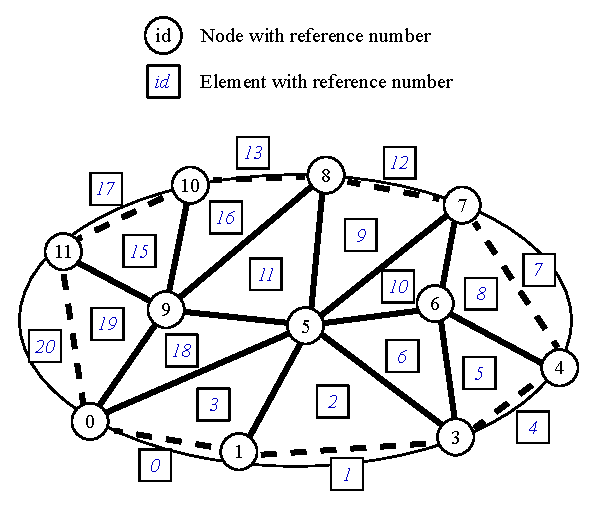
\includegraphics[width=\figwidth]{figures/FinleyMesh.eps}}
\caption{Subdivision of an Ellipse into triangles order 1 (\finleyelement{Tri3})}
\label{FINLEY FIG 0}
\end{figure}

\begin{figure}
\centerline{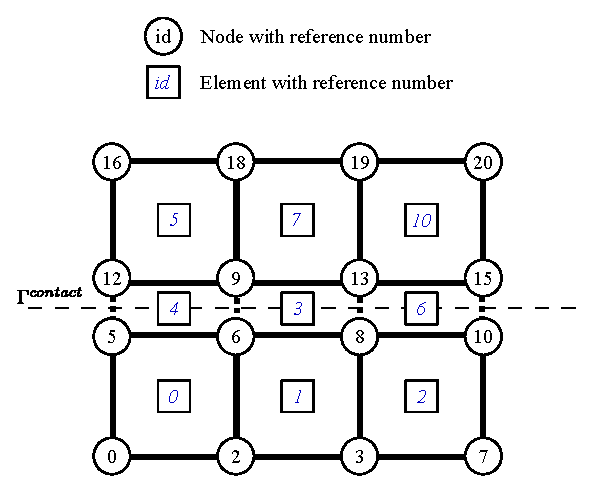
\includegraphics[width=\figwidth]{figures/FinleyContact.eps}}
\caption{Mesh around a contact region (\finleyelement{Rec4})}
\label{FINLEY FIG 01}
\end{figure}

\declaremodule{extension}{finley} \modulesynopsis{Solving linear, steady partial differential equations using
finite elements}

{\it finley} is a library of C functions solving linear, steady partial differential equations
\index{partial differential equations} (PDEs) or systems of PDEs using isoparametrical finite 
elements \index{FEM!isoparametrical}.
It supports unstructured, 1D, 2D and 3D meshes. The module \finley provides an access to the
library through the \LinearPDE class of \escript supporting its full functionality. {\it finley} 
is parallelized using the OpenMP \index{OpenMP} paradigm. 

\section{Formulation}

For a single PDE with a solution with a single component the linear PDE is defined in the
following form:
\begin{equation}\label{FINLEY.SINGLE.1}
\begin{array}{cl} &
\displaystyle{
\int\hackscore{\Omega} 
A\hackscore{jl} \cdot v\hackscore{,j}u\hackscore{,l}+ B\hackscore{j} \cdot v\hackscore{,j} u+ C\hackscore{l} \cdot v u\hackscore{,l}+D \cdot vu \; d\Omega }  \\
+ & \displaystyle{\int\hackscore{\Gamma} d \cdot vu \; d{\Gamma} } 
+  \displaystyle{\int\hackscore{\Gamma^{contact}} d^{contact} \cdot [v][u] \; d{\Gamma} } \\
= & \displaystyle{\int\hackscore{\Omega}  X\hackscore{j} \cdot v\hackscore{,j}+ Y \cdot v \; d\Omega }\\ 
+ & \displaystyle{\int\hackscore{\Gamma} y \cdot v \; d{\Gamma}}  + 
\displaystyle{\int\hackscore{\Gamma^{contact}} y^{contact}\cdot [v] \; d{\Gamma}} \\
\end{array}
\end{equation}

\section{Meshes}
To understand the usage of \finley one needs to have an understanding of how the finite element meshes
\index{FEM!mesh} are defined. \fig{FINLEY FIG 0} shows an example of the
subdivision of an ellipse into so called elements \index{FEM!elements} \index{element}. 
In this case, triangles have been used but other forms of subdivisions
can be constructed, e.g. into quadrilaterals or, in the three dimensional case, into tetrahedrons
and hexahedrons. The idea of the finite element method is to approximate the solution by a function
which is a polynomial of a certain order and is continuous across it boundary to neighbour elements.
In the example of \fig{FINLEY FIG 0} a linear polynomial is used on each triangle. As one can see, the triangulation
is quite a poor approximation of the ellipse. It can be improved by introducing a midpoint on each element edge then
positioning those nodes located on an edge expected to describe the boundary, onto the boundary.
In this case the triangle gets a curved edge which requires a parametrization of the triangle using a 
quadratic polynomial. For this case, the solution is also approximated by a piecewise quadratic polynomial
(which explains the name isoparametrical elements), see \Ref{Zienc,NumHand} for more details.   

The union of all elements defines the domain of the PDE.
Each element is defined by the nodes used to describe its shape. In \fig{FINLEY FIG 0} the element,
which has type \finleyelement{Tri3},
with element reference number $19$ \index{element!reference number} is defined by the nodes
with reference numbers $9$, $11$ and $0$ \index{node!reference number}. Notice that the order is counterclockwise. 
The coefficients of the PDE are evaluated at integration nodes with each individual element. 
For quadrilateral elements a Gauss quadrature scheme is used. In the case of triangular elements a 
modified form is applied. The boundary of the domain is also subdivided into elements. \index{element!face} In \fig{FINLEY FIG 0}
line elements with two nodes are used. The elements are also defined by their describing nodes, e.g.
the face element reference number $20$ which has type \finleyelement{Line2} is defined by the nodes
with the reference numbers $11$ and $0$. Again the order is crucial, if moving from the first
to second node the domain has to lie on the left hand side (in the case of a two dimension surface element
the domain has to lie on the left hand side when moving counterclockwise). If the gradient on the
surface of the domain is to be calculated rich face elements face to be used. Rich elements on a face
are identical to interior elements but with a modified order of nodes such that the 'first' face of the element aligns
with the surface of the domain. In \fig{FINLEY FIG 0}
elements of the type \finleyelement{Tri3Face} are used. 
The face element reference number $20$ as a rich face element is defined by the nodes
with reference numbers $11$, $0$ and $9$. Notice that the face element $20$ is identical to the
interior element $19$ except that, in this case, the order of the node is different to align the first
edge of the triangle (which is the edge starting with the first node) with the boundary of the domain.

Be aware that face elements and elements in the interior of the domain must match, i.e. a face element must be the face
of an interior element or, in case of a rich face element, it must be identical to an interior element.
If no face elements are specified
\finley implicitly assumes homogeneous natural boundary conditions \index{natural boundary conditions!homogeneous},
i.e. \var{d}=$0$ and \var{y}=$0$, on the entire boundary of the domain. For  
inhomogeneous natural boundary conditions \index{natural boundary conditions!inhomogeneous}, 
the boundary must be described by face elements. 

If discontinuities of the PDE solution are considered contact elements 
\index{element!contact}\index{contact conditions} are introduced to describe the contact region $\Gamma^{contact}$ 
even if $d^{contact}$ and $y^{contact}$ are zero. \fig{FINLEY FIG 01} shows a simple example of a mesh
of rectangular elements around a contact region $\Gamma^{contact}$ \index{element!contact}. 
The contact region is described by the
elements $4$, $3$ and $6$. Their element type is \finleyelement{Line2_Contact}. 
The nodes $9$, $12$, $6$, $5$ define contact element $4$, where the coordinates of nodes $12$ and $5$ and
nodes $4$ and $6$ are identical with the idea that nodes $12$ and $9$ are located above and 
nodes $5$ and $6$ below the contact region.  
Again, the order of the nodes within an element is crucial. There is also the option of using rich elements
if the gradient is to be calculated on the contact region. Similarly to the rich face elements 
these are constructed from two interior elements by reordering the nodes such that
the 'first' face of the element above and the 'first' face of the element below the 
contact regions line up.  The rich version of element 
$4$ is of type \finleyelement{Rec4Face_Contact} and is defined by the nodes $9$, $12$, $16$, $18$, $6$, $5$, $0$ and 
$2$.

\tab{FINLEY TAB 1} shows the interior element types and the corresponding element types to be used
on the face and contacts. \fig{FINLEY.FIG:1}, \fig{FINLEY.FIG:2} and \fig{FINLEY.FIG:4} show the ordering of
the nodes within an element.

\begin{table}
\begin{tablev}{l|llll}{textrm}{interior}{face}{rich face}{contact}{rich contact}
\linev{\finleyelement{Line2}}{\finleyelement{Point1}}{\finleyelement{Line2Face}}{\finleyelement{Point1_Contact}}{\finleyelement{Line2Face_Contact}}
\linev{\finleyelement{Line3}}{\finleyelement{Point1}}{\finleyelement{Line3Face}}{\finleyelement{Point1_Contact}}{\finleyelement{Line3Face_Contact}}
\linev{\finleyelement{Tri3}}{\finleyelement{Line2}}{\finleyelement{Tri3Face}}{\finleyelement{Line2_Contact}}{\finleyelement{Tri3Face_Contact}}
\linev{\finleyelement{Tri6}}{\finleyelement{Line3}}{\finleyelement{Tri6Face}}{\finleyelement{Line3_Contact}}{\finleyelement{Tri6Face_Contact}}
\linev{\finleyelement{Rec4}}{\finleyelement{Line2}}{\finleyelement{Rec4Face}}{\finleyelement{Line2_Contact}}{\finleyelement{Rec4Face_Contact}}
\linev{\finleyelement{Rec8}}{\finleyelement{Line3}}{\finleyelement{Rec8Face}}{\finleyelement{Line3_Contact}}{\finleyelement{Rec8Face_Contact}}
\linev{\finleyelement{Rec9}}{\finleyelement{Line3}}{\finleyelement{Rec9Face}}{\finleyelement{Line3_Contact}}{\finleyelement{Rec9Face_Contact}}
\linev{\finleyelement{Tet4}}{\finleyelement{Tri6}}{\finleyelement{Tet4Face}}{\finleyelement{Tri6_Contact}}{\finleyelement{Tet4Face_Contact}}
\linev{\finleyelement{Tet10}}{\finleyelement{Tri9}}{\finleyelement{Tet10Face}}{\finleyelement{Tri9_Contact}}{\finleyelement{Tet10Face_Contact}}
\linev{\finleyelement{Hex8}}{\finleyelement{Rec4}}{\finleyelement{Hex8Face}}{\finleyelement{Rec4_Contact}}{\finleyelement{Hex8Face_Contact}}
\linev{\finleyelement{Hex20}}{\finleyelement{Rec8}}{\finleyelement{Hex20Face}}{\finleyelement{Rec8_Contact}}{\finleyelement{Hex20Face_Contact}}
\end{tablev}
\caption{Finley elements and corresponding elements to be used on domain faces and contacts.
The rich types have to be used if the gradient of function is to be calculated on faces and contacts, respectively.}
\label{FINLEY TAB 1}
\end{table}

The native \finley file format is defined as follows.
Each node \var{i} has \var{dim} spatial coordinates \var{Node[i]}, a reference number
\var{Node_ref[i]}, a degree of freedom \var{Node_DOF[i]} and tag \var{Node_tag[i]}.
In most cases \var{Node_DOF[i]}=\var{Node_ref[i]} however, for periodic boundary conditions,
\var{Node_DOF[i]} is chosen differently, see example below. The tag can be used to mark nodes sharing
the same properties. Element \var{i} is defined by the \var{Element_numNodes} nodes \var{Element_Nodes[i]}
which is a list of node reference numbers. The order is crucial.
It has a reference number \var{Element_ref[i]} and a tag \var{Element_tag[i]}. The tag 
can be used to mark elements  sharing the same properties. For instance elements above 
a contact region are marked with $2$ and elements below a contact region are marked with $1$. 
\var{Element_Type} and \var{Element_Num} give the element type and the number of elements in the mesh.
Analogue notations are used for face and contact elements. The following Python script
prints the mesh definition in the \finley file format:
\begin{python}
print "%s\n"%mesh_name
# node coordinates:
print "%dD-nodes %d\n"%(dim,numNodes)
for i in range(numNodes): 
   print "%d %d %d"%(Node_ref[i],Node_DOF[i],Node_tag[i])
   for j in range(dim): print " %e"%Node[i][j]
   print "\n"
# interior elements
print "%s %d\n"%(Element_Type,Element_Num)
for i in range(Element_Num):
   print "%d %d"%(Element_ref[i],Element_tag[i])
   for j in range(Element_numNodes): print " %d"%Element_Nodes[i][j]
   print "\n"
# face elements
print "%s %d\n"%(FaceElement_Type,FaceElement_Num)
for i in range(FaceElement_Num):
   print "%d %d"%(FaceElement_ref[i],FaceElement_tag[i])
   for j in range(FaceElement_numNodes): print " %d"%FaceElement_Nodes[i][j]
   print "\n"
# contact elements
print "%s %d\n"%(ContactElement_Type,ContactElement_Num)
for i in range(ContactElement_Num):
   print "%d %d"%(ContactElement_ref[i],ContactElement_tag[i])
   for j in range(ContactElement_numNodes): print " %d"%ContactElement_Nodes[i][j]
   print "\n"
# point sources (not supported yet)
write("Point1 0",face_element_type,numFaceElements)
\end{python}

The following example of a mesh file defines the mesh shown in \fig{FINLEY FIG 01}:
\begin{verbatim}
Example 1
2D Nodes 16
0   0 0 0.   0.
2   2 0 0.33 0.
3   3 0 0.66 0.
7   4 0 1.   0.
5   5 0 0.   0.5
6   6 0 0.33 0.5
8   8 0 0.66 0.5
10 10 0 1.0  0.5
12 12 0 0.   0.5
9   9 0 0.33 0.5
13 13 0 0.66 0.5
15 15 0 1.0  0.5
16 16 0 0.   1.0
18 18 0 0.33 1.0
19 19 0 0.66 1.0
20 20 0 1.0  1.0
Rec4 6
 0 1  0  2  6  5
 1 1  2  3  8  6
 2 1  3  7 10  8
 5 2 12  9 18 16
 7 2 13 19 18  9
10 2 20 19 13 15
Line2 0
Line2_Contact 3
 4 0  9 12  6 5
 3 0 13  9  8 6
 6 0 15 13 10 8
Point1 0
\end{verbatim}
Notice that the order in which the nodes and elements are given is arbitrary.
In the case that rich contact elements are used the contact element section gets
 the form
\begin{verbatim}
Rec4Face_Contact 3
 4 0  9 12 16 18  6  5  0  2
 3 0 13  9 18 19  8  6  2  3
 6 0 15 13 19 20 10  8  3  7
\end{verbatim}
Periodic boundary condition \index{boundary conditions!periodic} can be introduced by altering \var{Node_DOF}.
It allows identification of nodes even if they have different physical locations. For instance, to
enforce periodic boundary conditions at the face $x_0=0$ and $x_0=1$ one identifies
the degrees of freedom for nodes $0$, $5$, $12$ and $16$ with the degrees of freedom for
$7$, $10$, $15$ and $20$, respectively. The node section of the \finley mesh gets now the form:  
\begin{verbatim}
2D Nodes 16
0   0 0 0.   0.
2   2 0 0.33 0.
3   3 0 0.66 0.
7   0 0 1.   0.
5   5 0 0.   0.5
6   6 0 0.33 0.5
8   8 0 0.66 0.5
10  5 0 1.0  0.5
12 12 0 0.   0.5
9   9 0 0.33 0.5
13 13 0 0.66 0.5
15 12 0 1.0  0.5
16 16 0 0.   1.0
18 18 0 0.33 1.0
19 19 0 0.66 1.0
20 16 0 1.0  1.0
\end{verbatim}



%%%%%%%%%%%%%%%%%%%%%%%%%%%%%%%%%%%%%%%%%%%%%%%%%%%%%%%%%%%%%%%%%%%%%%%%%%%%%%
% Copyright (c) 2003-2018 by The University of Queensland
% http://www.uq.edu.au
%
% Primary Business: Queensland, Australia
% Licensed under the Apache License, version 2.0
% http://www.apache.org/licenses/LICENSE-2.0
%
% See CREDITS file for contributors and development history
%
%%%%%%%%%%%%%%%%%%%%%%%%%%%%%%%%%%%%%%%%%%%%%%%%%%%%%%%%%%%%%%%%%%%%%%%%%%%%%%

\setlength{\unitlength}{1mm}

\newsavebox{\HLa}
\savebox{\HLa}(0,0)
  {\put(0,0){\circle*{2}}
   \thicklines \put(1,0){\line(1,0){28}}
   \put(30,0){\circle*{2}} }

\newsavebox{\HLathin}
\savebox{\HLathin}(0,0)
  {\put(0,0){\circle{2}}
   \thinlines \put(1,0){\line(1,0){28}}
   \put(30,0){\circle{2}} }

\newsavebox{\VLa}
\savebox{\VLa}(0,30)
  {\put(0,0){\circle*{2}}
   \thicklines \put(0,1){\line(0,1){28}}
   \put(0,30){\circle*{2}} }

\newsavebox{\VLathin}
\savebox{\VLathin}(0,30)
  {\put(0,0){\circle{2}}
   \thinlines \put(0,1){\line(0,1){28}}
   \put(0,30){\circle{2}} }

\newsavebox{\SLax}
\savebox{\SLax}(0,30)
  {\thicklines \put(0,0){\line(-1,1){30}}
   \put(0,0){\circle*{2}}
   \put(-30,30){\circle*{2}} }

\newsavebox{\SLaa}
\savebox{\SLaa}(0,15)
  {\thicklines \put(0,0){\line(-4,3){20}}
   \put(0,0){\circle*{2}}
   \put(-20,15){\circle*{2}} }

\newsavebox{\SLab}
\savebox{\SLab}(0,-15)
  {\thicklines \put(0,0){\line(-4,-3){20}}
   \put(0,0){\circle*{2}}
   \put(-20,-15){\circle*{2}} }

\newsavebox{\SLabthin}
\savebox{\SLabthin}(0,-15)
  {\thinlines \put(-0.7,-0.7){\line(-4,-3){18.7}}
   \put(0,0){\circle{2}}
   \put(-20,-15){\circle{2}} }

\newsavebox{\SLac}
\savebox{\SLac}(0,15)
  {\thicklines \put(0,0){\line(-2,3){10}}
   \put(0,0){\circle*{2}}
   \put(-10,15){\circle*{2}} }

\newsavebox{\SLacthin}
\savebox{\SLacthin}(0,15)
  {\thinlines \put(0,0){\line(-2,3){9.4}}
   \put(0,0){\circle{2}}
   \put(-10,15){\circle{2}} }


\newsavebox{\HLd}
\savebox{\HLd}(0,0)
  {\put(0,0){\circle*{2}}
   \put(10,0){\circle*{2}}
   \thicklines \put(1,0){\line(1,0){28}}
   \put(20,0){\circle*{2}}
   \put(30,0){\circle*{2}} }

\newsavebox{\HLdthin}
\savebox{\HLdthin}(0,0)
  {\put(0,0){\circle{2}}
   \put(10,0){\circle{2}}
   \thinlines \multiput(1,0)(10,0){3}{\line(1,0){8}}
   \put(20,0){\circle{2}}
   \put(30,0){\circle{2}} }

\newsavebox{\VLd}
\savebox{\VLd}(0,30)
  {\put(0,0){\circle*{2}}
   \put(0,10){\circle*{2}}
   \thicklines \put(0,1){\line(0,1){28}}
   \put(0,20){\circle*{2}}
   \put(0,30){\circle*{2}} }

\newsavebox{\VLdthin}
\savebox{\VLdthin}(0,30)
  {\put(0,0){\circle{2}}
   \put(0,10){\circle{2}}
   \thinlines \multiput(0,1)(0,10){3}{\line(0,1){8}}
   \put(0,20){\circle{2}}
   \put(0,30){\circle{2}} }

\newsavebox{\SLf}
\savebox{\SLf}(0,30)
  {\thicklines \put(0,0){\line(-1,1){30}}
   \put(0,0){\circle*{2}}
   \put(-10,10){\circle*{2}}
   \put(-20,20){\circle*{2}}
   \put(-30,30){\circle*{2}} }

\newsavebox{\SLad}
\savebox{\SLad}(0,15)
  {\thicklines \put(0,0){\line(-4,3){20}}
   \put(0,0){\circle*{2}}
   \put(-6.66,5){\circle*{2}}
   \put(-13.33,10){\circle*{2}}
   \put(-20,15){\circle*{2}} }

\newsavebox{\SLbd}
\savebox{\SLbd}(0,-15)
  {\thicklines \put(0,0){\line(-4,-3){20}}
   \put(0,0){\circle*{2}}
   \put(-6.66,-5){\circle*{2}}
   \put(-13.33,-10){\circle*{2}}
   \put(-20,-15){\circle*{2}} }

\newsavebox{\SLbdthin}
\savebox{\SLbdthin}(0,-15)
  {\thinlines \multiput(-0.7,-0.7)(-6.66,-5){3}{\line(-4,-3){5.1}}
   \put(0,0){\circle{2}}
   \put(-6.66,-5){\circle{2}}
   \put(-13.33,-10){\circle{2}}
   \put(-20,-15){\circle{2}} }

\newsavebox{\SLcd}
\savebox{\SLcd}(0,15)
  {\thicklines \put(0,0){\line(-2,3){10}}
   \put(0,0){\circle*{2}}
   \put(-3.33,5){\circle*{2}}
   \put(-6.66,10){\circle*{2}}
   \put(-10,15){\circle*{2}} }

\newsavebox{\SLcdthin}
\savebox{\SLcdthin}(0,15)
  {\thinlines \multiput(-0.6,0.8)(-3.33,5){3}{\line(-2,3){2.35}}
   \put(0,0){\circle{2}}
   \put(-3.33,5){\circle{2}}
   \put(-6.66,10){\circle{2}}
   \put(-10,15){\circle{2}} }

\newsavebox{\HLe}
\savebox{\HLe}(0,0)
  {\put(0,0){\circle*{2}}
   \put(15,0){\circle*{2}}
   \thicklines \put(1,0){\line(1,0){28}}
   \put(30,0){\circle*{2}} }

\newsavebox{\HLethin}
\savebox{\HLethin}(0,0)
  {\put(0,0){\circle{2}}
   \put(15,0){\circle{2}}
   \thinlines \multiput(1,0)(15,0){2}{\line(1,0){13}}
   \put(30,0){\circle{2}} }

\newsavebox{\VLe}
\savebox{\VLe}(0,30)
  {\put(0,0){\circle*{2}}
   \put(0,15){\circle*{2}}
   \thicklines \put(0,1){\line(0,1){28}}
   \put(0,30){\circle*{2}} }

\newsavebox{\VLethin}
\savebox{\VLethin}(0,30)
  {\put(0,0){\circle{2}}
   \put(0,15){\circle{2}}
   \thinlines \multiput(0,1)(0,15){2}{\line(0,1){13}}
   \put(0,30){\circle{2}} }

\newsavebox{\SLe}
\savebox{\SLe}(0,30)
  {\thicklines \put(0,0){\line(-1,1){30}}
   \put(0,0){\circle*{2}}
   \put(-15,15){\circle*{2}}
   \put(-30,30){\circle*{2}} }

\newsavebox{\SLae}
\savebox{\SLae}(0,15)
  {\thicklines \put(0,0){\line(-4,3){20}}
   \put(0,0){\circle*{2}}
   \put(-10,7.5){\circle*{2}}
   \put(-20,15){\circle*{2}} }

\newsavebox{\SLbe}
\savebox{\SLbe}(0,-15)
  {\thicklines \put(0,0){\line(-4,-3){20}}
   \put(0,0){\circle*{2}}
   \put(-10,-7.5){\circle*{2}}
   \put(-20,-15){\circle*{2}} }

\newsavebox{\SLbethin}
\savebox{\SLbethin}(0,-15)
  {\thinlines \multiput(-0.7,-0.7)(-10,-7.5){2}{\line(-4,-3){8.4}}
   \put(0,0){\circle{2}}
   \put(-10,-7.5){\circle{2}}
   \put(-20,-15){\circle{2}} }

\newsavebox{\SLce}
\savebox{\SLce}(0,15)
  {\thicklines \put(0,0){\line(-2,3){10}}
   \put(0,0){\circle*{2}}
   \put(-5,7.5){\circle*{2}}
   \put(-10,15){\circle*{2}} }

\newsavebox{\SLcethin}
\savebox{\SLcethin}(0,15)
  {\thinlines \multiput(-0.6,0.8)(-5,7.5){2}{\line(-2,3){3.9}}
   \put(0,0){\circle{2}}
   \put(-5,7.5){\circle{2}}
   \put(-10,15){\circle{2}} }

%=====================================================================
%
%   order 1
%   -------
%

\begin{figure}
\begin{center}
\begin{picture}(150,160) \thicklines

\put(20,155){\circle*{2}}
\put(15,145){\parbox[t]{45mm}
             \finleyelement{Point1}}

\put(90,155){\usebox{\HLa}}
\put(90,145){\parbox[t]{45mm}
             \finleyelement{Line2} }

\put(10,95){\usebox{\HLa}}
\put(40,95){\usebox{\SLax}}
\put(10,95){\usebox{\VLa}}
\put(10,85){\parbox[t]{45mm}
             \finleyelement{Tri3} }

\put(90,95){\usebox{\HLa}}
\put(90,125){\usebox{\HLa}}
\put(90,95){\usebox{\VLa}}
\put(120,95){\usebox{\VLa}}
\put(90,85){\parbox[t]{45mm}
             \finleyelement{Rec4} }

\put(10,20){\usebox{\HLa}}
\put(40,20){\usebox{\SLax}}
\put(10,20){\usebox{\VLa}}
\put(40,20){\usebox{\SLac}}
\put(30,35){\usebox{\SLabthin}}
\put(30,35){\usebox{\SLaa}}
\put(10,10 ){\parbox[t]{45mm}
             \finleyelement{Tet4} }

\put(90,20){\usebox{\HLa}}
\put(90,50){\usebox{\HLa}}
\put(90,20){\usebox{\VLa}}
\put(120,20){\usebox{\VLa}}
\put(110,35){\usebox{\SLabthin}}
\put(140,35){\usebox{\SLab}}
\put(110,65){\usebox{\SLab}}
\put(140,65){\usebox{\SLab}}
\put(110,35){\usebox{\HLathin}}
\put(110,65){\usebox{\HLa}}
\put(110,35){\usebox{\VLathin}}
\put(140,35){\usebox{\VLa}}
\put(90,10 ){\parbox[t]{45mm}
             \finleyelement{Hex8} }

% numbering the lines:
 % Point
\put(19,158){{\it 1}}
% line
\put(89,158){{\it 1}} 
\put(119,158){{\it 2}}
% Triangle
\put(6,124){{\it 3}}
\put(6,94){{\it 1}}
\put(43,94){{\it 2}}
% quadrilateral
\put(86,124){{\it 4}}
\put(86,94){{\it 1}}
\put(123,124){{\it 3}}
\put(123,94){{\it 2}}
% Tetrahedron
\put(6,49){{\it 4}}
\put(6,19){{\it 1}}
\put(43,19){{\it 2}}
\put(33,34){{\it 3}}
% Hexahedron
\put(86,49){{\it 5}} 
\put(86,19){{\it 1}}
\put(123,49){{\it 6}}
\put(123,19){{\it 2}}
\put(106,64){{\it 8}}
\put(106,34){{\it 4}}
\put(143,64){{\it 7}}
\put(143,34){{\it 3}}
\end{picture}
\caption{\label{FINLEY.FIG:1} Elements of order 1}
\end{center}
\end{figure}
%=====================================================================
%
%
%   order 2
%   -------
%   (boxes in 'fesubelm')


\begin{figure}
\begin{center}
\setlength{\unitlength}{1mm}
\begin{picture}(150,160) \thicklines

\put(20,155){\circle*{2}}
\put(15,145){\parbox[t]{45mm}
             \finleyelement{Point1} }

\put(90,155){\usebox{\HLe}}
\put(90,145){\parbox[t]{45mm}
             \finleyelement{Line3} and \finleyelement{Line3Macro} }

\put(10,95){\usebox{\HLe}}
\put(40,95){\usebox{\SLe}}
\put(10,95){\usebox{\VLe}}
\put(10,85){\parbox[t]{45mm}
             \finleyelement{Tri6} }

\put(90,95){\usebox{\HLe}}
\put(90,125){\usebox{\HLe}}
\put(90,95){\usebox{\VLe}}
\put(120,95){\usebox{\VLe}}
\put(90,85){\parbox[t]{45mm}
             \finleyelement{Rec8} }

\put(10,20){\usebox{\HLe}}
\put(40,20){\usebox{\SLe}}
\put(10,20){\usebox{\VLe}}
\put(40,20){\usebox{\SLce}}
\put(30,35){\usebox{\SLbethin}}
\put(30,35){\usebox{\SLae}}
\put(10,10 ){\parbox[t]{45mm}
             \finleyelement{Tet10} and \finleyelement{Tet10Macro}}

\put(90,20){\usebox{\HLe}}
\put(90,50){\usebox{\HLe}}
\put(90,20){\usebox{\VLe}}
\put(120,20){\usebox{\VLe}}
\put(110,35){\usebox{\SLbethin}}
\put(140,35){\usebox{\SLbe}}
\put(110,65){\usebox{\SLbe}}
\put(140,65){\usebox{\SLbe}}
\put(110,35){\usebox{\HLethin}}
\put(110,65){\usebox{\HLe}}
\put(110,35){\usebox{\VLethin}}
\put(140,35){\usebox{\VLe}}
\put(90,10 ){\parbox[t]{45mm}
             \finleyelement{Hex20} }


% numbering the lines:
% Point
\put(19,158){{\it 1}} 
% line
\put(89,158){{\it 1}} 
\put(104,158){{\it 3}}
\put(119,158){{\it 2}}
% Triangle
\put(6,124){{\it 3}} 
\put(6,109){{\it 6}}
\put(6,94){{\it 1}}
\put(28,109){{\it 5}}
\put(43,94){{\it 2}}
\put(24,90){{\it 4}}
% quaTrilateral
\put(104,90){{\it 5}} 
\put(86,124){{\it 4}}
\put(86,109){{\it 8}}
\put(86,94){{\it 1}}
\put(104,128){{\it 7}}
\put(123,124){{\it 3}}
\put(123,109){{\it 6}}
\put(123,94){{\it 2}}
% Tetrahedron
\put(24,15){{\it 5}} 
\put(6,49){{\it 4}}
\put(6,34){{\it 8}}
\put(6,19){{\it 1}}
\put(21,34){{\it 9}}
\put(43,19){{\it 2}}
\put(16,26.5){{\it 7}}
\put(38,26.5){{\it 6}}
\put(33,34){{\it 3}}
\put(22.5,41.5){{\it 10}}
% Hexahedron
\put(104,15){{\it 9}} 
\put(86,49){{\it 5}}
\put(85,34){{\it 13}}
\put(86,19){{\it 1}}
\put(104,52){{\it 17}}
\put(123,49){{\it 6}}
\put(115,37){{\it 14}}
\put(123,19){{\it 2}}
\put(125,37){{\it 11}}
\put(106,64){{\it 8}}
\put(112,46){{\it 16}}
\put(106,34){{\it 4}}
\put(124,68){{\it 19}}
\put(143,64){{\it 7}}
\put(142,49){{\it 15}}
\put(143,34){{\it 3}}
\put(94.5,26.5){{\it 12}}
\put(132.5,26.5){{\it 10}}
\put(94.5,56.5){{\it 20}}
\put(132.5,56.5){{\it 18}}

\end{picture}
\caption{\label{FINLEY.FIG:2} Elements of order 2 and macro elements}
\end{center}
\end{figure}

%
% additional elements
%
\begin{figure}
\begin{center}
\begin{picture}(50,50) \thicklines
\put(10,10){\usebox{\HLe}}
\put(10,40){\usebox{\HLe}}
\put(10,10){\usebox{\VLe}}
\put(40,10){\usebox{\VLe}}
\put(25,25){\circle*{2}}
% \put(50,085){\parbox[t]{45mm}
%              \finleyelement{Rec9} and  \finleyelement{Rec9Macro}}
\put(24,5){{\it 5}}
\put(6,39){{\it 4}}
\put(6,24){{\it 8}}
\put(6,9){{\it 1}}
\put(24,43){{\it 7}}
\put(43,43){{\it 3}}
\put(43,25){{\it 6}}
\put(43,9){{\it 2}}
\put(24,20){{\it 9}}
\end{picture}
\caption{\label{FINLEY.FIG:4}\finleyelement{Rec9} and  \finleyelement{Rec9Macro}}
\end{center}
\end{figure}


\subsection{Linear Solvers in \LinearPDE}
Currently \finley supports the linear solvers \PCG, \GMRES, \PRESTWENTY and \BiCGStab. 
For \GMRES the options \var{truncation} and \var{restart} of the \method{getSolution} can be
used to control the truncation and restart during iteration. Default values are
\var{truncation}=5 and \var{restart}=20.
The default solver is \BiCGStab  but if the symmetry flag is set \PCG is the default solver.
\finley supports the solver options \var{iter_max} which specifies the maximum number of iterations steps,
\var{verbose}=\True or \False and \var{preconditioner}=\constant{JACOBI} or \constant {ILU0}.
In some installations \finley supports the \Direct solver and the
solver options \var{reordering}=\constant{util.NO_REORDERING}, 
\constant{util.MINIMUM_FILL_IN} or \constant{util.NESTED_DISSECTION} (default is \constant{util.NO_REORDERING}),
\var{drop_tolerance} specifying the threshold for values to be dropped in the 
incomplete elimination process (default is 0.01) and \var{drop_storage} specifying the maximum increase 
in storage allowed in the 
incomplete elimination process (default is 1.20).

\subsection{Functions}
\begin{funcdesc}{Mesh}{fileName,integrationOrder=-1}
creates a \Domain object form the FEM mesh defined in 
file \var{fileName}. The file must be given the \finley file format.
If \var{integrationOrder} is positive, a numerical integration scheme
chosen which is accurate on each element up to a polynomial of
degree \var{integrationOrder} \index{integration order}. Otherwise
an appropriate integration order is chosen independently.
\end{funcdesc}

\begin{funcdesc}{Rectangle}{n0,n1,order=1,l0=1.,l1=1., integrationOrder=-1, \\
  periodic0=\False,periodic1=\False,useElementsOnFace=\False,optimize=\False}
Generates a \Domain object representing a two dimensional rectangle between
$(0,0)$ and $(l0,l1)$ with orthogonal edges. The rectangle is filled with
\var{n0} elements along the $x_0$-axis and
\var{n1} elements along the $x_1$-axis. 
For \var{order}=1 and \var{order}=2
\finleyelement{Rec4} and  
\finleyelement{Rec8} are used, respectively. 
In the case of \var{useElementsOnFace}=\False,
\finleyelement{Line2} and  
\finleyelement{Line3} are used to subdivide the edges of the rectangle, respectively. 
In the case of \var{useElementsOnFace}=\True (this option should be used if gradients
are calculated on domain faces),
\finleyelement{Rec4Face} and  
\finleyelement{Rec8Face} are used on the edges, respectively.  
If \var{integrationOrder} is positive, a numerical integration scheme
chosen which is accurate on each element up to a polynomial of
degree \var{integrationOrder} \index{integration order}. Otherwise
an appropriate integration order is chosen independently. If
\var{periodic0}=\True, periodic boundary conditions \index{periodic boundary conditions}
along the $x_0$-directions are enforced. That means when for any solution of a PDE solved by \finley
the value on the line $x_0=0$ will be identical to the values on $x_0=\var{l0}$.
Correspondingly,
\var{periodic1}=\False sets periodic boundary conditions
in $x_1$-direction.
If \var{optimize}=\True mesh node relabeling will be attempted to reduce the computation and also ParMETIS will be used to improve the mesh partition if running on multiple CPUs with MPI.
\end{funcdesc}

\begin{funcdesc}{Brick}{n0,n1,n2,order=1,l0=1.,l1=1.,l2=1., integrationOrder=-1, \\
  periodic0=\False,periodic1=\False,periodic2=\False,useElementsOnFace=\False,optimize=\False}
Generates a \Domain object representing a three dimensional brick between
$(0,0,0)$ and $(l0,l1,l2)$ with orthogonal faces. The brick is filled with
\var{n0} elements along the $x_0$-axis, 
\var{n1} elements along the $x_1$-axis and 
\var{n2} elements along the $x_2$-axis. 
For \var{order}=1 and \var{order}=2
\finleyelement{Hex8} and  
\finleyelement{Hex20} are used, respectively. 
In the case of \var{useElementsOnFace}=\False,
\finleyelement{Rec4} and  
\finleyelement{Rec8} are used to subdivide the faces of the brick, respectively. 
In the case of \var{useElementsOnFace}=\True (this option should be used if gradients
are calculated on domain faces),
\finleyelement{Hex8Face} and  
\finleyelement{Hex20Face} are used on the brick faces, respectively.  
If \var{integrationOrder} is positive, a numerical integration scheme
chosen which is accurate on each element up to a polynomial of
degree \var{integrationOrder} \index{integration order}. Otherwise
an appropriate integration order is chosen independently. If
\var{periodic0}=\True, periodic boundary conditions \index{periodic boundary conditions}
along the $x_0$-directions are enforced. That means when for any solution of a PDE solved by \finley
the value on the plane $x_0=0$ will be identical to the values on $x_0=\var{l0}$. Correspondingly,
\var{periodic1}=\False and \var{periodic2}=\False sets periodic boundary conditions
in $x_1$-direction and $x_2$-direction, respectively.
If \var{optimize}=\True mesh node relabeling will be attempted to reduce the computation and also ParMETIS will be used to improve the mesh partition if running on multiple CPUs with MPI.
\end{funcdesc}

\begin{funcdesc}{GlueFaces}{meshList,safetyFactor=0.2,tolerance=1.e-13}
Generates a new \Domain object from the list \var{meshList} of \finley meshes.
Nodes in face elements whose difference of coordinates is less then \var{tolerance} times the 
diameter of the domain are merged. The corresponding face elements are removed from the mesh.  

TODO: explain \var{safetyFactor} and show an example.
\end{funcdesc}

\begin{funcdesc}{JoinFaces}{meshList,safetyFactor=0.2,tolerance=1.e-13}
Generates a new \Domain object from the list \var{meshList} of \finley meshes.
Face elements whose nodes coordinates have difference is less then \var{tolerance} times the 
diameter of the domain are combined to form a contact element \index{element!contact} 
The corresponding face elements are removed from the mesh.  

TODO: explain \var{safetyFactor} and show an example.
\end{funcdesc}


\input{troubleshooting}
\makemodindex

\printindex
%% $Id$
\documentclass{manual}

% grab the handy definitions and \usepackage statements etc
% $Id$

\usepackage{epsfig}
\usepackage{graphicx,color}
\usepackage{makeidx}  % handle the index properly
\usepackage{xspace}   % handle spaces after commands more nicely
% use the ams math stuff, as it makes the maths easier to code, and
% nicer output than the standard LaTeX stuff
\usepackage{amsmath,amsfonts,amssymb} % this is handy for mathematicians and physicists
			              % see http://www.ams.org/tex/amslatex.html
\usepackage{alltt}   % handy verbatim stuff


% define some handy commands for escript stuff
\newcommand{\ESyS}{\module{ESyS}\xspace}
\newcommand{\escript}{\module{escript}\xspace}
\newcommand{\finley}{\module{finley}\xspace}
\newcommand{\linearPDE}{\class{linearPDE}\xspace}
\newcommand{\Data}{\class{Data}\xspace}

% default width for figures
\newcommand{\figwidth}{100mm}

% commands useful in cross-referencing
\newcommand {\Ref}[1] {Reference~\cite{#1}}
\newcommand {\Sec}[1] {Section~\ref{#1}}
\newcommand {\App}[1] {Appendix~\ref{#1}}
\newcommand {\Chap}[1] {Chapter~\ref{#1}}
\newcommand {\etal} {\emph{~et~al.}}
\newcommand {\fig}[1] {Figure~\ref{#1}}
\newcommand {\eqn}[1] {Equation~(\ref{#1})} 
\newcommand {\tab}[1] {Table~\ref{#1}}

% improved version of caption handling
\usepackage{ccaption}
\captionnamefont{\scshape}
\captionstyle{}
\makeatletter
\renewcommand{\fnum@figure}[1]{\quad\small\textsc{\figurename~\thefigure}:}
\renewcommand{\@makecaption}[2]{%
\vskip\abovecaptionskip
\sbox\@tempboxa{#1: #2}%
\ifdim \wd\@tempboxa >\hsize
  \def\baselinestretch{1}\@normalsize
  #1: #2\par
  \def\baselinestretch{1.5}\@normalsize
\else
  \global \@minipagefalse
  \hb@xt@\hsize{\hfil\box\@tempboxa\hfil}%
\fi
\vskip\belowcaptionskip}
\makeatother

\usepackage{fancyvrb}  % fancy verbatim stuff.  Needed so code below goes
%%% this code grabbed from the PyScript docs
%%% pyscript.sourceforge.net

% --------------------------------------------------------------
% Code format within \Verb
% --------------------------------------------------------------

\definecolor{pycolor}{rgb}{0,0.4,0}

\DefineVerbatimEnvironment{python}{Verbatim}
{frame=leftline,framerule=.5mm,rulecolor=\color{pycolor},
formatcom=\color{pycolor}\small,fontshape=rm}

%\DefineShortVerb[formatcom=\color{dgreen}\small,fontshape=sl]{\|}

\RecustomVerbatimCommand{\Verb}{Verb}{formatcom=\color{pycolor}\small,fontshape=rm}

%%% end of grabbed code

% this is for when one uses pdflatex and therefore needs to load pdf
% figures into \includegraphics
\ifpdf
	\DeclareGraphicsExtensions{.pdf}  % this command defined in graphicx
	\pdfcompresslevel=9  % 0: no compression, 9: highest compression
			     % or, set compress_level 9 in file pdftex.cfg
\else
	\DeclareGraphicsExtensions{.eps}
\fi


% title, author, etc stuff
\title{ESyS Users Guide}

\author{Lutz Gross (Editor)}
\authoraddress{
Earth Systems Science Computational Centre (ESSCC) \\
The University of Queensland \\
Australia \\
Email: \email{esys@access.edu.au}
}                                                                                         
\date{\today}      
\release{$Id$}
\setreleaseinfo{} 
\setshortversion{}

\makeindex

% the actual start of the document
\begin{document}

\maketitle


%%%%%%%%%%%%%%%%%%%%%%%%%%%%%%%%%%%%%%%%%%%%%%%%%%%%%%%%%%%%%%%%%%%%%%%%%%%%%%
% Copyright (c) 2003-2026 by the esys.escript Group
% https://github.com/LutzGross/esys-escript.github.io
%
% Primary Business: Queensland, Australia
% Licensed under the Apache License, version 2.0
% http://www.apache.org/licenses/LICENSE-2.0
%
% See CREDITS file for contributors and development history
%
%%%%%%%%%%%%%%%%%%%%%%%%%%%%%%%%%%%%%%%%%%%%%%%%%%%%%%%%%%%%%%%%%%%%%%%%%%%%%%

\begin{center}
Copyright (c) 2003-2026 esys.escript Group \\
\url{https://github.com/LutzGross/esys-escript.github.io}\\
Primary Business: Queensland, Australia\\
Licensed under the Apache License, version 2.0\\
\url{http://www.apache.org/licenses/LICENSE-2.0}\\
This work was supported by the AuScope National Collaborative Research
Infrastructure Strategy, the Queensland State Government and The University
of Queensland.
\end{center}



\begin{abstract}
This document is a guide of how to use the \ESyS software and
associated tools.
\end{abstract}

\tableofcontents

% $Id$


\chapter{Introduction}
\label{INTRO}

\subsection{Getting the software}


\escript, \ESyS, all freely available.  Where do people get \finley from?



\begin{enumerate}
 \item general structure 
 \item how to get the software
 \item a few words about the general structure
\item installation
\end{enumerate}

\subsection{Acknowlegements}
\begin{itemize}
\item Margeret Kahn Australian Nationional Unversity, Canberra.
\end{itemize}


%%%%%%%%%%%%%%%%%%%%%%%%%%%%%%%%%%%%%%%%%%%%%%%%%%%%%%%%%%%%%%%%%%%%%%%%%%%%%%
% Copyright (c) 2003-2026 by the esys.escript Group
% https://github.com/LutzGross/esys-escript.github.io
%
% Primary Business: Queensland, Australia
% Licensed under the Apache License, version 2.0
% http://www.apache.org/licenses/LICENSE-2.0
%
% See CREDITS file for contributors and development history
%
%%%%%%%%%%%%%%%%%%%%%%%%%%%%%%%%%%%%%%%%%%%%%%%%%%%%%%%%%%%%%%%%%%%%%%%%%%%%%%

\section{The First Steps}\label{FirstSteps} 
This chapter is an introduction on how to use \escript to solve 
a partial differential equation\index{partial differential equation} (PDE\index{partial differential equation!PDE}).
We assume you are at least a little familiar with \PYTHON.
The knowledge presented in the \PYTHON tutorial at \url{https://docs.python.org/2/tutorial/} is more than sufficient.

The PDE\index{partial differential equation} we wish to solve is the Poisson equation\index{Poisson equation} 
\begin{equation}
    -\Delta u=f 
    \label{eq:FirstSteps.1}
\end{equation}
for the solution $u$. The function $f$ is the given right hand side. The domain of interest, denoted by $\Omega$,
is the unit square 
\begin{equation}
\Omega=[0,1]^2=\{ (x_0;x_1) | 0\le x_{0} \le 1 \mbox{ and } 0\le x_{1} \le 1 \}
\label{eq:FirstSteps.1b}
\end{equation}
The domain is shown in \fig{fig:FirstSteps.1}.
\begin{figure}[ht]
    \centerline{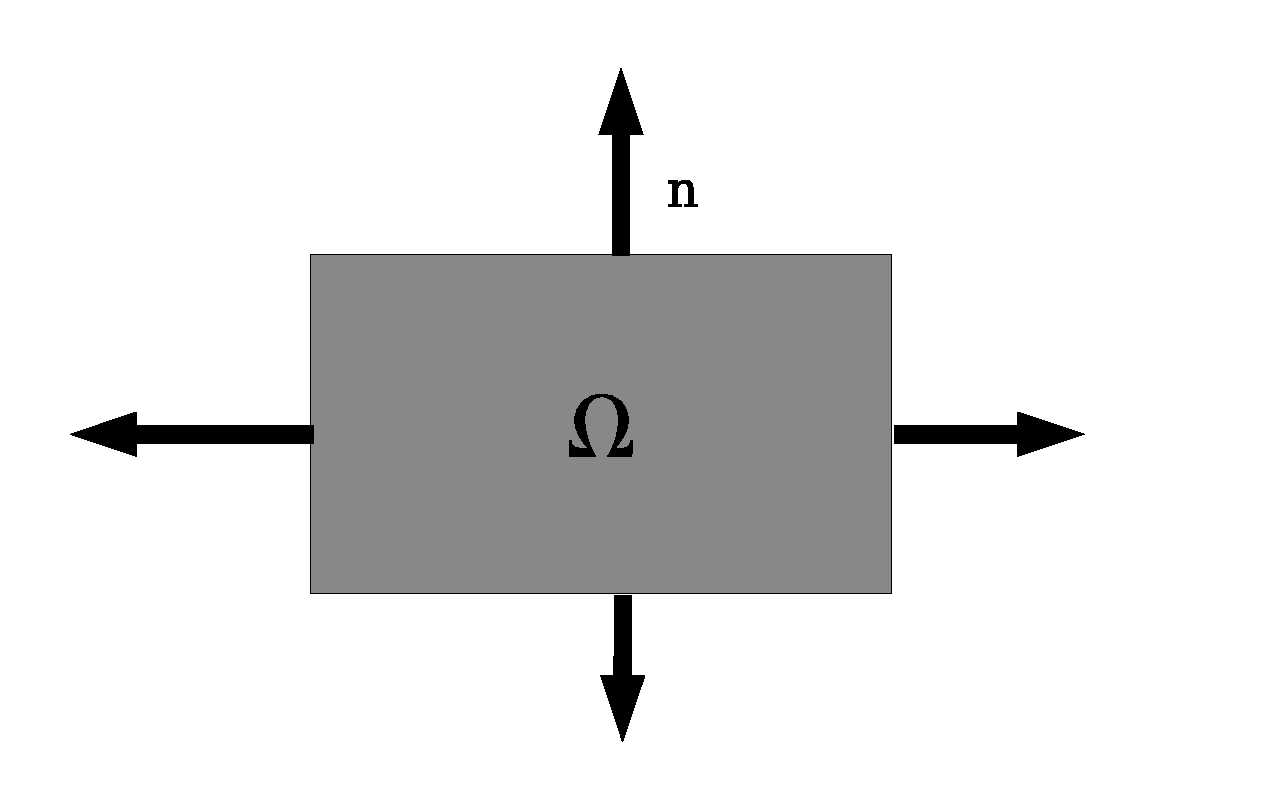
\includegraphics{FirstStepDomain}}
    \caption{Domain $\Omega=[0,1]^2$ with outer normal field $n$.}
    \label{fig:FirstSteps.1}
\end{figure}

$\Delta$ denotes the Laplace operator\index{Laplace operator}, which is defined by
\begin{equation}
\Delta u = (u_{,0})_{,0}+(u_{,1})_{,1}
\label{eq:FirstSteps.1.1}
\end{equation}
where, for any function $u$ and any direction $i$, $u_{,i}$
denotes the partial derivative \index{partial derivative} of $u$ with respect
to $i$.\footnote{You may be more familiar with the Laplace
operator\index{Laplace operator} being written as $\nabla^2$, and written in
the form
\begin{equation*}
    \nabla^2 u = \nabla^t \cdot \nabla u =  \frac{\partial^2 u}{\partial x_0^2} 
    + \frac{\partial^2 u}{\partial  x_1^2}
\end{equation*}
and \eqn{eq:FirstSteps.1} as
\begin{equation*}
    -\nabla^2 u = f
\end{equation*}
}
Basically, in the subindex of a function, any index to the right of the comma denotes a spatial derivative with respect 
to the index. To get a more compact form we will write $u_{,ij}=(u_{,i})_{,j}$
which leads to
\begin{equation}
\Delta u = u_{,00}+u_{,11}=\sum_{i=0}^2 u_{,ii}
\label{eq:FirstSteps.1.1b}
\end{equation}
We often find that use
of nested $\sum$ symbols makes formulas cumbersome, and we use the more
compact Einstein summation convention\index{summation convention}. This 
drops the $\sum$ sign and assumes that a summation is performed over any repeated index.
For instance, 
\begin{eqnarray}
x_{i}y_{i}=\sum_{i=0}^2 x_{i}y_{i}   \\
x_{i}u_{,i}=\sum_{i=0}^2 x_{i}u_{,i}   \\
u_{,ii}=\sum_{i=0}^2 u_{,ii} \\
x_{ij}u_{i,j}=\sum_{j=0}^2\sum_{i=0}^2 x_{ij}u_{i,j}   \\
\label{eq:FirstSteps.1.1c}
\end{eqnarray}
With the summation convention we can write the Poisson equation \index{Poisson equation} as
\begin{equation}
- u_{,ii} =1 
\label{eq:FirstSteps.1.sum}
\end{equation}
where $f=1$ in this example.

On the boundary of the domain $\Omega$ the normal derivative $n_{i} u_{,i}$
of the solution $u$ shall be zero, i.e. $u$ shall fulfill
the homogeneous Neumann boundary condition\index{Neumann
boundary condition!homogeneous}
\begin{equation}
n_{i} u_{,i}= 0 \;.
\label{eq:FirstSteps.2}
\end{equation}
$n=(n_{i})$ denotes the outer normal field
of the domain, see \fig{fig:FirstSteps.1}. Remember that we 
apply the Einstein summation convention \index{summation convention}, i.e. $n_{i} u_{,i}= n_{0} u_{,0} +%
n_{1} u_{,1}$.\footnote{Some readers may be more familiar with the
notation $\frac{\partial u}{\partial n} = n_{i} u_{,i}=\mathbf{n}\cdot \nabla u$.}
The Neumann boundary condition of \eqn{eq:FirstSteps.2} should be fulfilled on the
set $\Gamma^N$, the top and right edge of the domain:
\begin{equation}
    \Gamma^N=\{(x_0;x_1) \in \Omega | x_{0}=1 \mbox{ or } x_{1}=1  \}
    \label{eq:FirstSteps.2b}
\end{equation}
On the bottom and the left edge of the domain, defined
as 
\begin{equation}
    \Gamma^D=\{(x_0;x_1) \in \Omega | x_{0}=0 \mbox{ or } x_{1}=0  \}
    \label{eq:FirstSteps.2c}
\end{equation}
the solution shall be identical to zero:
\begin{equation}
    u=0 \; .
    \label{eq:FirstSteps.2d}
\end{equation}
A homogeneous Dirichlet boundary
condition\index{Dirichlet boundary condition!homogeneous}.
The partial differential equation in \eqn{eq:FirstSteps.1.sum} together
with Neumann  \eqn{eq:FirstSteps.2} and 
Dirichlet boundary conditions in \eqn{eq:FirstSteps.2d} form a so-called
boundary value
problem\index{boundary value problem} (BVP\index{boundary value problem!BVP})
for the unknown function~$u$. 

\begin{figure}[ht]
    \centerline{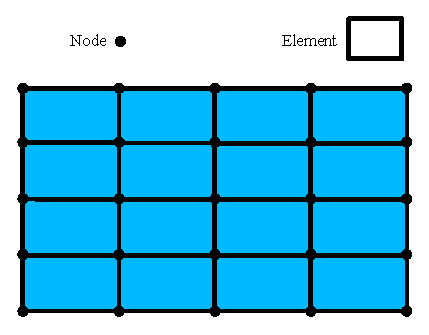
\includegraphics{FirstStepMesh}}
    \caption{Mesh of $4 \times 4$ elements on a rectangular domain. Here
    each element is a quadrilateral and described by four nodes, namely
    the corner points. The solution is interpolated by a bi-linear
    polynomial.}
    \label{fig:FirstSteps.2}
\end{figure}

In general the BVP\index{boundary value problem!BVP} cannot be solved
analytically and numerical methods are used to construct an
approximation of the solution $u$.
Here we will use the finite element method\index{finite element method}
(FEM\index{finite element method!FEM}).
The basic idea is to fill the domain with a set of points called nodes.
The solution is approximated by its values on the nodes\index{finite element method!nodes}.
Moreover, the domain is subdivided into smaller sub-domains called
elements\index{finite element method!element}.
On each element the solution is represented by a polynomial of a certain
degree through its values at the nodes located in the element.
The nodes and their connection through elements is called a
mesh\index{finite element method!mesh}. \fig{fig:FirstSteps.2} shows an
example of a FEM mesh with four elements in the $x_0$ and four elements
in the $x_1$ direction over the unit square.
For more details we refer the reader to the literature, for instance \Refe{Zienc,NumHand}.

The \escript solver we want to use to solve this problem is embedded into the \PYTHON interpreter language.
So you can solve the problem interactively but you will learn quickly that it
is more efficient to use scripts which can be edited with your favorite editor.
To enter the escript environment, use the \program{run-escript}
command\footnote{\program{run-escript} is not available under Windows.
If you run under Windows you can just use the \program{python} command and the
\env{OMP_NUM_THREADS} environment variable to control the number of threads.}:
\begin{verbatim}
run-escript
\end{verbatim}
which will pass you on to the \PYTHON prompt
\begin{verbatim}
Python 2.7.6 (default, Mar 22 2014, 15:40:47) 
[GCC 4.8.2] on linux2
Type "help", "copyright", "credits" or "license" for more information.
>>> 
\end{verbatim}
Here you can use all available \PYTHON commands and language features\footnote{Throughout our examples, we use the python 3 form of 
print. That is, print(1) instead of print 1.}, for instance
\begin{python}
  >>> x=2+3
  >>> print("2+3=",x)
  2+3= 5
\end{python}
We refer to the \PYTHON user's guide if you are not familiar with \PYTHON.

\escript provides the class \Poisson to define a Poisson equation\index{Poisson equation}.
(We will discuss a more general form of a PDE\index{partial differential equation!PDE} 
that can be defined through the \LinearPDE class later.)
The instantiation of a \Poisson class object requires the specification of the domain $\Omega$.
In \escript \Domain class objects are used to describe the geometry of a
domain but it also contains information about the discretization methods and
the solver used to solve the PDE.
Here we use the FEM\index{finite element method} library \finley.
The following statements create the \Domain object \var{mydomain} from the 
\finley function \method{Rectangle}:
\begin{python}
  from esys.finley import Rectangle
  mydomain = Rectangle(l0=1.,l1=1.,n0=40, n1=20)
\end{python}
In this case the domain is a rectangle with the lower left corner at point $(0,0)$
and the upper right corner at $(\var{l0},\var{l1})=(1,1)$.
The arguments \var{n0} and \var{n1} define the number of elements in $x_{0}$ and
$x_{1}$-direction respectively. For more details on \method{Rectangle} and
other \Domain generators see \Chap{chap:finley}, \Chap{chap:ripley}, and
\Chap{chap:speckley}.

The following statements define the \Poisson class object \var{mypde} with domain \var{mydomain} and
the right hand side $f$ of the PDE to constant $1$: 
\begin{python}
  from esys.escript.linearPDEs import Poisson
  mypde = Poisson(mydomain)
  mypde.setValue(f=1)
\end{python}
We have not specified any boundary condition but the \Poisson class implicitly
assumes homogeneous Neuman boundary conditions\index{Neumann boundary condition!homogeneous} defined by \eqn{eq:FirstSteps.2}.
With this boundary condition the BVP\index{boundary value problem!BVP} we have
defined has no unique solution.
In fact, with any solution $u$ and any constant $C$ the function $u+C$ becomes
a solution as well.
We have to add a Dirichlet boundary condition\index{Dirichlet boundary condition}.
This is done by defining a characteristic function\index{characteristic function}
which has positive values at locations $x=(x_{0},x_{1})$
where Dirichlet boundary condition is set and $0$ elsewhere.
In our case of $\Gamma^D$ defined by \eqn{eq:FirstSteps.2c}, we need to
construct a function \var{gammaD} which is positive for the cases $x_{0}=0$ or $x_{1}=0$.
To get an object \var{x} which contains the coordinates of the nodes in the domain use
\begin{python}
  x=mydomain.getX() 
\end{python}
The method \method{getX} of the \Domain \var{mydomain} gives access to locations
in the domain defined by \var{mydomain}.
The object \var{x} is actually a \Data object which will be discussed in
\Chap{ESCRIPT CHAP} in more detail.
What we need to know here is that \var{x} has \Rank (number of dimensions) and
a \Shape (list of dimensions) which can be viewed by calling the \method{getRank} and \method{getShape} methods:
\begin{python}
  print("rank ",x.getRank(),", shape ",x.getShape())
\end{python}
This will print something like
\begin{python}
  rank 1, shape (2,)
\end{python}
The \Data object also maintains type information which is represented by the 
\FunctionSpace of the object. For instance
\begin{python}
  print(x.getFunctionSpace())
\end{python}
will print 
\begin{python}
  Finley_Nodes [ContinuousFunction(domain)] on FinleyMesh 
\end{python}
which tells us that the coordinates are stored on the nodes of (rather than on
points in the interior of) a Finley mesh.
To get the  $x_{0}$ coordinates of the locations we use the statement 
\begin{python}
  x0=x[0]
\end{python}
Object \var{x0} is again a \Data object now with \Rank $0$ and \Shape $()$.
It inherits the \FunctionSpace from \var{x}:
\begin{python}
  print(x0.getRank(), x0.getShape(), x0.getFunctionSpace())
\end{python}
will print
\begin{python}
  0 () Finley_Nodes [ContinuousFunction(domain)] on FinleyMesh
\end{python}
We can now construct a function \var{gammaD} which is only non-zero on the
bottom and left edges of the domain with
\begin{python}
  from esys.escript import whereZero
  gammaD=whereZero(x[0])+whereZero(x[1])
\end{python}

\code{whereZero(x[0])} creates a function which equals $1$ where \code{x[0]} is (almost) equal to zero and $0$ elsewhere. 
Similarly, \code{whereZero(x[1])} creates a function which equals $1$ where \code{x[1]} is equal to zero and $0$ elsewhere.
The sum of the results of \code{whereZero(x[0])} and \code{whereZero(x[1])}
gives a function on the domain \var{mydomain} which is strictly positive where $x_{0}$ or $x_{1}$ is equal to zero.
Note that \var{gammaD} has the same \Rank, \Shape and \FunctionSpace as \var{x0} used to define it.
So from 
\begin{python}
  print(gammaD.getRank(), gammaD.getShape(), gammaD.getFunctionSpace())
\end{python}
one gets 
\begin{python}
  0 () Finley_Nodes [ContinuousFunction(domain)] on FinleyMesh
\end{python}
An additional parameter \var{q} of the \code{setValue} method of the \Poisson
class defines the characteristic function\index{characteristic function} of
the locations of the domain where the homogeneous Dirichlet boundary condition\index{Dirichlet boundary condition!homogeneous} is set.
The complete definition of our example is now:
\begin{python}
  from esys.escript.linearPDEs import Poisson
  x = mydomain.getX()
  gammaD = whereZero(x[0])+whereZero(x[1])
  mypde = Poisson(domain=mydomain)
  mypde.setValue(f=1,q=gammaD)
\end{python}
The first statement imports the \Poisson class definition from the \linearPDEs module.
To get the solution of the Poisson equation defined by \var{mypde} we just have to call its \method{getSolution} method. 

Now we can write the script to solve our Poisson problem
\begin{python}
  from esys.escript import *
  from esys.escript.linearPDEs import Poisson
  from esys.finley import Rectangle
  # generate domain:
  mydomain = Rectangle(l0=1.,l1=1.,n0=40, n1=20)
  # define characteristic function of Gamma^D
  x = mydomain.getX()
  gammaD = whereZero(x[0])+whereZero(x[1])
  # define PDE and get its solution u
  mypde = Poisson(domain=mydomain)
  mypde.setValue(f=1, q=gammaD)
  u = mypde.getSolution()
\end{python}
The question is what we do with the calculated solution \var{u}.
Besides postprocessing, e.g. calculating the gradient or the average value,
which will be discussed later, plotting the solution is one of the things you
might want to do.
\escript offers two ways to do this, both based on external modules or packages.
The first option uses the \MATPLOTLIB module which allows plotting of 2D
results relatively quickly from within the \PYTHON script, see~\cite{matplotlib}.
However, there are limitations when using this tool, especially for large
problems and when solving three-dimensional problems.
Therefore, \escript provides functionality to export data as files which can
subsequently be read by third-party software packages such as
\mayavi\cite{mayavi} or \VisIt~\cite{VisIt}.

\subsection{Plotting Using \MATPLOTLIB}
The \MATPLOTLIB module provides a simple and easy-to-use way to visualize PDE
solutions (or other \Data objects).
To hand over data from \escript to \MATPLOTLIB the values need to be mapped onto
a rectangular grid. We will make use of the \numpy module for this.

First we need to create a rectangular grid which is accomplished by the following statements:
\begin{python}
  import numpy
  x_grid = numpy.linspace(0., 1., 50)
  y_grid = numpy.linspace(0., 1., 50)
\end{python}
\var{x_grid} is an array defining the x coordinates of the grid while
\var{y_grid} defines the y coordinates of the grid.
In this case we use $50$ points over the interval $[0,1]$ in both directions. 

Now the values created by \escript need to be interpolated to this grid.
We will use the \SCIPY \function{interpolate.griddata} function to do this.
Spatial coordinates are easily extracted as a \var{list} by
\begin{python}
  x=mydomain.getX()[0].toListOfTuples()
  y=mydomain.getX()[1].toListOfTuples()
\end{python}
In principle we can apply the same \member{toListOfTuples} method to extract the values from the PDE solution \var{u}.
However, we have to make sure that the \Data object we extract the values from
uses the same \FunctionSpace as we have used when extracting \var{x} and \var{y}.
We apply the \function{interpolation} to \var{u} before extraction to achieve this:
\begin{python}
  z=interpolate(u, mydomain.getX().getFunctionSpace())
\end{python}
The values in \var{z} are the values at the points with the coordinates given by \var{x} and \var{y}.
These values are interpolated to the grid defined by \var{x_grid} and \var{y_grid} by using
\begin{python}
   import scipy.interpolate
   z_grid = scipy.interpolate.griddata((x,y),z,(x_grid[None,:],y_grid[:,None]),'linear')
\end{python}
Now \var{z_grid} gives the values of the PDE solution \var{u} at the grid which can be plotted using \function{contourf}:
\begin{python}
  import matplotlib
  matplotlib.pyplot.contourf(x_grid, y_grid, z_grid, 5)
  matplotlib.pyplot.savefig("u.png")
\end{python}
Here we use 5 contours. The last statement writes the plot to the file \file{u.png} in the PNG format.
Alternatively, one can use 
\begin{python}
  matplotlib.pyplot.contourf(x_grid, y_grid, z_grid, 5)
  matplotlib.pyplot.show()
\end{python}
which gives an interactive browser window.

\begin{figure}
\centerline{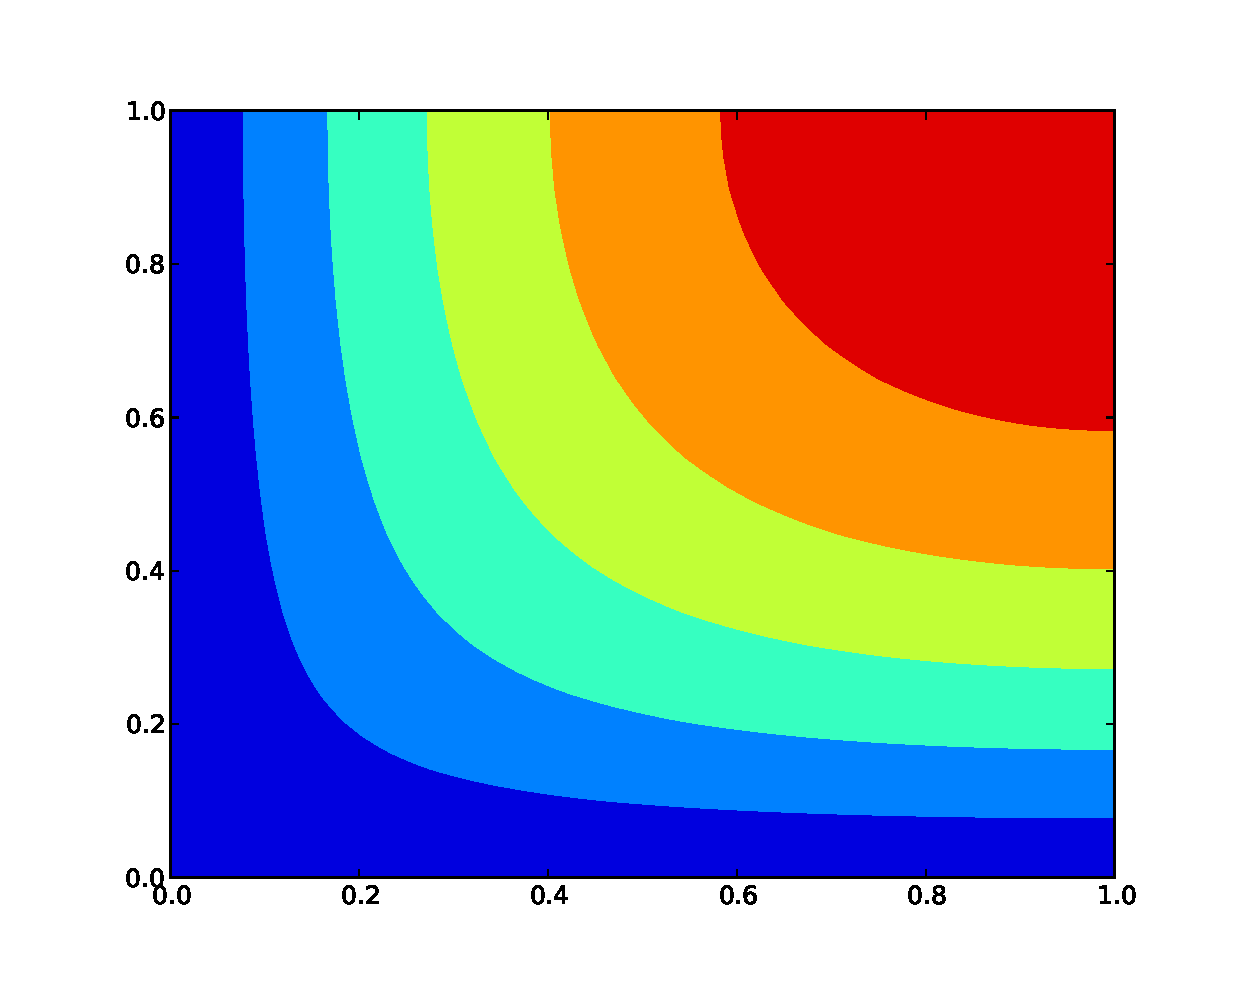
\includegraphics[width=\figwidth]{FirstStepResultMATPLOTLIB}}
\caption{Visualization of the Poisson Equation Solution for $f=1$ using \MATPLOTLIB}
\label{fig:FirstSteps.3b}
\end{figure}

Now we can write the script to solve our Poisson problem
\begin{python}
  from esys.escript import *
  from esys.escript.linearPDEs import Poisson
  from esys.finley import Rectangle
  import scipy.interpolate
  import numpy
  import matplotlib

  import pylab
  # generate domain:
  mydomain = Rectangle(l0=1.,l1=1.,n0=40, n1=20)
  # define characteristic function of Gamma^D
  x = mydomain.getX()
  gammaD = whereZero(x[0])+whereZero(x[1])
  # define PDE and get its solution u
  mypde = Poisson(domain=mydomain)
  mypde.setValue(f=1,q=gammaD)
  u = mypde.getSolution()
  # interpolate u to a matplotlib grid:
  x_grid = numpy.linspace(0.,1.,50)
  y_grid = numpy.linspace(0.,1.,50)
  x=mydomain.getX()[0].toListOfTuples()
  y=mydomain.getX()[1].toListOfTuples()
  z=interpolate(u,mydomain.getX().getFunctionSpace()).toListOfTuples()
  z_grid = scipy.interpolate.griddata((x,y),z,(x_grid[None,:],y_grid[:,None]),'linear')
  # interpolate u to a rectangular grid:
  matplotlib.pyplot.contourf(x_grid, y_grid, z_grid, 5)
  matplotlib.pyplot.savefig("u.png")
\end{python}
The entire code is available as \file{poisson_matplotlib.py} in the \ExampleDirectory.
You can run the script using the {\it escript} environment
\begin{verbatim}
run-escript poisson_matplotlib.py
\end{verbatim}
This will create a file called \file{u.png}, see \fig{fig:FirstSteps.3b}.
For details on the usage of the \MATPLOTLIB module we refer to the documentation~\cite{matplotlib}.

As pointed out, \MATPLOTLIB is restricted to the two-dimensional case and
should be used for small problems only.
It can not be used under \MPI as the \member{toListOfTuples} method is not
safe under \MPI\footnote{The phrase 'safe under \MPI' means that a program
will produce correct results when run on more than one processor under \MPI.}.

\begin{figure}
\centerline{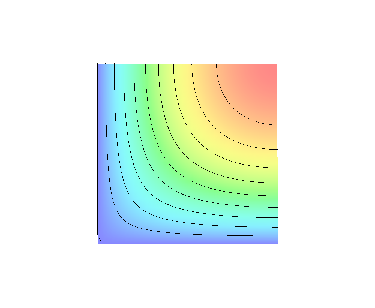
\includegraphics[width=\figwidth]{FirstStepResult}}
\caption{Visualization of the Poisson Equation Solution for $f=1$}
\label{fig:FirstSteps.3}
\end{figure}

\subsection{Visualization using export files}

As an alternative to \MATPLOTLIB, {\it escript} supports exporting data to
\VTK and \SILO files which can be read by visualization tools such as
\mayavi\cite{mayavi} and \VisIt~\cite{VisIt}. This method is \MPI safe and
works with large 2D and 3D problems.

To write the solution \var{u} of the Poisson problem in the \VTK file format
to the file \file{u.vtu} one needs to add:
\begin{python}
  from esys.weipa import saveVTK
  saveVTK("u.vtu", sol=u)
\end{python}
This file can then be opened in a \VTK compatible visualization tool where the
solution is accessible by the name {\it sol}. Similarly,
\begin{python}
  from esys.weipa import saveSilo
  saveSilo("u.silo", sol=u)
\end{python}
will write \var{u} to a \SILO file if escript was compiled with support for
LLNL's \SILO library.

The Poisson problem script is now 
\begin{python}
  from esys.escript import *
  from esys.escript.linearPDEs import Poisson
  from esys.finley import Rectangle
  from esys.weipa import saveVTK
  # generate domain:
  mydomain = Rectangle(l0=1.,l1=1.,n0=40, n1=20)
  # define characteristic function of Gamma^D
  x = mydomain.getX()
  gammaD = whereZero(x[0])+whereZero(x[1])
  # define PDE and get its solution u
  mypde = Poisson(domain=mydomain)
  mypde.setValue(f=1,q=gammaD)
  u = mypde.getSolution()
  # write u to an external file
  saveVTK("u.vtu",sol=u)
\end{python}
The entire code is available as \file{poisson_vtk.py} in the \ExampleDirectory.

You can run the script using the {\it escript} environment and visualize the
solution using \mayavi:
\begin{verbatim}
run-escript poisson_vtk.py
mayavi2 -d u.vtu -m Surface
\end{verbatim}
The result is shown in \fig{fig:FirstSteps.3}.


% $Id$
\chapter{How to Solve The Diffusion Equation}
\label{DIFFUSION CHAP}

\begin{figure}
\centerline{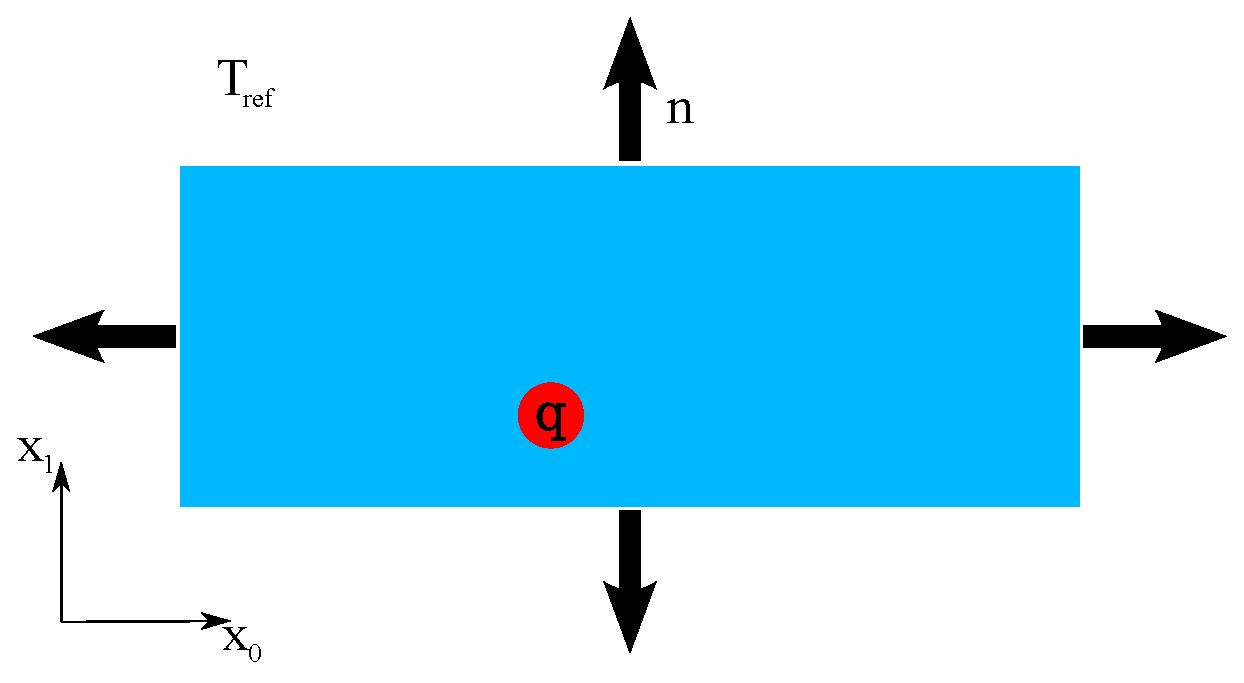
\includegraphics[width=\figwidth]{DiffusionDomain}}
\caption{Temperature Diffusion Problem with Circular Heat Source}
\label{DIFFUSION FIG 1}
\end{figure}

\begin{figure}
\centerline{
\includegraphics[width=\figwidth]{DiffusionRes1}}
\centerline{
\includegraphics[width=\figwidth]{DiffusionRes16}}
\centerline{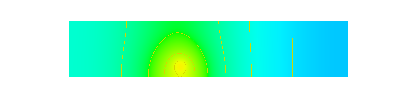
\includegraphics[width=\figwidth]{DiffusionRes32}}
\centerline{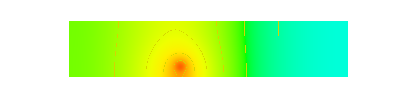
\includegraphics[width=\figwidth]{DiffusionRes48}}
\caption{Results of the Temperture Diffusion Problem for Time Steps $1$ $16$, $32$ and $48$.}
\label{DIFFUSION FIG 2}
\end{figure}


\section{\label{DIFFUSION OUT SEC}Outline}
In this chapter we will discuss how to solve the time depeneded-temperature diffusion\index{diffusion equation} within
a block of material. Within the block there is a heat source which drives the temperature diffusion.
On the surface energy can radiate into the surrounding environment.
\fig{DIFFUSION FIG 1} shows the configuration.

In the next \Sec{DIFFUSION TEMP SEC} we will present the relevant model. A 
time integration scheme is introduced to calculate the temperature at given time nodes $t^{(n)}$. 
We will see that at time step a so-called Helmholtz equation \index{Helmholtz equation} has to be solved. 
The implementation iof a Helmholtz equation solver will be discussed in \Sec{DIFFUSION HELM SEC}. 
In Section~\ref{DIFFUSION TRANS SEC} the solver of the Helmholtz equation is used to build a
solver for the temperature diffusion problem. 

\section{\label{DIFFUSION TEMP SEC}Temperature Diffusion}

The temperature $T$ is a function of its location in the domain and time $t>0$. The governing equation
in the interior of the domain is given by
\begin{equation}
\rho c\hackscore p T\hackscore{,t} - (\kappa T\hackscore{,i})\hackscore{,i} = q
\label{DIFFUSION TEMP EQ 1}
\end{equation}
where $\rho c\hackscore p$ and $\kappa$ are given material constants. In case of a composite
material the parameters are depending on the their location in the domain. $q$ is
a heat source (or sink) within the domain. We are using Einstein summation convention \index{summation convention} 
as introduced in \Chap{FirstSteps}. In our case we assume $q$ to be equal to a constant $q^{c}$
on a circle or sphere with center $x^c$ and radius $r$ and $0$ elsewhere:
\begin{equation}
q(x,t)=
\left\{ 
\begin{array}{lcl}
q^c  & & \|x-x^c\| \le r \\
     & \mbox{if} \\
0    &  & \mbox{else} \\
\end{array}
\right.
\label{DIFFUSION TEMP EQ 1b}
\end{equation}
for all $x$ in the domain and all time  $t>0$.

On the surface of the domain we are 
are specifying a radiation condition 
which precribes the normal component of the flux $J\hackscore i= \kappa T\hackscore{,i}$ to be proportional
to the difference of the current temperature to the surrounding temperature $T\hackscore{ref}$:    
\begin{equation}
 \kappa T\hackscore{,i} n\hackscore i = \eta (T\hackscore{ref}-T) 
\label{DIFFUSION TEMP EQ 2}
\end{equation}
$\eta$ is a given material coefficient depending on the material and the surrounding medium. 
As usual $n_i$ is the $i$-th component of the outer normal field \index{outer normal field}
at the surface of the domain. 

To solve the the time depended \eqn{DIFFUSION TEMP EQ 1} the initial temperature at time 
$t=0$ has to be given. Here we assume that the initial temperature is the surrounding temperature:
\begin{equation}
T(x,0)=T\hackscore{ref} 
\label{DIFFUSION TEMP EQ 4}
\end{equation}
for all $x$ in the domain. It is pointed out that 
the initial conditions is fullfilling the 
boundary condition defined by \eqn{DIFFUSION TEMP EQ 2}. 

The temperature is calculated discrete time nodes $t^{(n)}$ where 
$t^{(0)}=0$ and  $t^{(n)}=t^{(n-1)}+h$ where $h>0$ is the step size which is assumed to be constant. 
In the following the upper index ${(n)}$ is refering to a value at time $t^{(n)}$. The simplest
and most robust scheme to approximate the time derivative of the the temperature is the 
\index{backward Euler} scheme, see~\cite{XXX} for alternatives. The backward Euler scheme bases
on the Taylor expansion
\begin{equation}
T^{(n-1)}\approx T^{(n)}+T\hackscore{,t}^{(n)}(t^{(n-1)}-t^{(n)})
=T^{(n-1)} + h \cdot T\hackscore{,t}^{(n)}
\label{DIFFUSION TEMP EQ 6}
\end{equation}
which is inserted into \eqn{DIFFUSION TEMP EQ 1}. By separating the terms at 
$t^{(n)}$ and  $t^{(n-1)}$ one gets for $n=1,2,3\ldots$
\begin{equation}
\frac{\rho c\hackscore p}{h} T^{(n)} - (\kappa T^{(n)}\hackscore{,i})\hackscore{,i} = q +  \frac{\rho c\hackscore p}{h} T^{(n-1)}
\label{DIFFUSION TEMP EQ 7}
\end{equation}
where $T^{(0)}=T\hackscore{ref}$ is taken form the initial condition given by \eqn{DIFFUSION TEMP EQ 4}.
Together with the natural boundary condition from \eqn{DIFFUSION TEMP EQ 2}.
this forms a boundary value problem that has to be solved for each time step. 
As a first step to implement a solver for the temperature diffusion problem we will 
first implement a solver for the  boundary value problem that has to be solved at each time step.

\section{\label{DIFFUSION HELM SEC}Helmholtz Problem}
The partial differential equation to be solved for $T^{(n)}$ has the form 
\begin{equation}
\omega u  - (\kappa u\hackscore{,i})\hackscore{,i} = f
\label{DIFFUSION HELM EQ 1}
\end{equation}
where $u$ plays the role of $T^{(n)}$ and we set
\begin{equation}
\omega=\frac{\rho c\hackscore p}{h} \mbox{ and } f=q+\frac{\rho c\hackscore p}{h}T^{(n-1)} \;.
\label{DIFFUSION HELM EQ 1b}
\end{equation}
With $g=\eta T\hackscore{ref}$ the radiation condition defined by \eqn{DIFFUSION TEMP EQ 2}
takes the form 
\begin{equation}
\kappa u\hackscore{,i} n\hackscore{i} =  g - \eta u\mbox{ on } \Gamma
\label{DIFFUSION HELM EQ 2}
\end{equation}
The partial differential 
\eqn{DIFFUSION HELM EQ 1} together with boundary conditions of \eqn{DIFFUSION HELM EQ 2}
is called a Helmholtz equation \index{Helmholtz equation}. 

We want to use the \LinearPDE class provided by \escript to define and solve a general linear PDE such as the 
Helmholtz equation. We have used a special case of the \LinearPDE class, namely the
\Poisson class already in \Chap{FirstSteps}. 
Here we will write our own specialized class of the \LinearPDE to solve the Helmholtz equation. 

The general form of a single PDE that can be handeled by the \LinearPDE class is 
\begin{equation}\label{EQU.FEM.1}
-(A\hackscore{jl} u\hackscore{,l})\hackscore{,j}+D u =Y \; .
\end{equation}
The general form and systems is discussed in \Sec{SEC LinearPDE}.  
$A$, $D$ and $Y$ are the known coeffecients of the PDE \index{partial differential equation!coefficients}. 
Notice that $A$ is a matrix or tensor of order 2 and $D$ and $Y$ are scalar. 
They may be constant or may depend on their 
location in the domain but must not depend on the unknown solution $u$. 
The following natural boundary conditions \index{boundary condition!natural} that
are used in the \LinearPDE class have the form
\begin{equation}\label{EQU.FEM.2}
n\hackscore{j}A\hackscore{jl} u\hackscore{,l}+du=y  \;.
\end{equation}
where, as usual, $n$ denotes the outer normal field on the surface of the domain. Notice that 
the coefficient $A$ is already used in the PDE in \eqn{EQU.FEM.1}. $d$ and $y$ are given scalar coefficients.

By inpecting the Helmholtz equation \index{Helmholtz equation} 
we can easily assign values to the coefficients in the 
general PDE of the \LinearPDE class:
\begin{equation}\label{DIFFUSION HELM EQ 3}
\begin{array}{llllll}
A\hackscore{ij}=\kappa \delta\hackscore{ij} & D=\omega & Y=f \\
d=\eta & y= g &  \\
\end{array}
\end{equation}
$\delta\hackscore{ij}$ is the Kronecker symbol \index{Kronecker symbol} defined by $\delta=\hackscore{ij}=1$ for
$i=j$ and $0$ otherwise.

We want to implement a 
new class which we will call \class{Helmholtz} that provides the same methods like the \LinearPDE class but
is defined through the coefficeints $\kappa$, $\omega$, $f$, $\eta$, 
$g$ rather than the general form given by \eqn{EQU.FEM.1}.
Python's
mechanism of inhertence allows doing this in a very easy way. 
The advantage is that our new \class{Helmholtz} can be used in any context 
that works with a \LinearPDE class but with an easier interface to define the PDE.
This improves reuasablity as well as maintainability of program codes.

We want to implement a 
new class which we will call \class{Helmholtz} that provides the same methods like the \LinearPDE class but
is defined through the coefficeints $\kappa$, $\omega$, $f$, $\alpha$, 
$g$ rather than the general form given by \eqn{EQU.FEM.1}. 
Python's mechanism of subclasses allows doing this in a very easy way.
The \Poisson class of the \linearPDEsPack module,
which we have already used in \Chap{FirstSteps}, is in fact a subclass of the 
\LinearPDE class. That means that it all methods (such as the \method{getSolution})
from the parent class \LinearPDE are defined for any \Poisson object. However, new
methods can be added and methods of the parent class can be redefined. In fact,
the \Poisson class redefines the \method{setValue} of the \LinearPDE class which is called to assign 
values to the coefficients of the PDE. This is exactly what we will do when we define 
our new \class{Helmholtz} class:
\begin{python}
from esys.linearPDEs import LinearPDE
import numarray
class Helmholtz(LinearPDE)
   def setValue(self,kappa=0,omega=1,f=0,eta=0,g=0)
        self._setValue(A=kappa*numarray.identity(self.getDim()),D=omega,Y=f,d=eta,y=g)
\end{python}
\code{class Helmholtz(linearPDE)} declares the new \class{Helmholtz} class as a subclass 
of the \LinearPDE which have imported in the first line of the script. 
We add the method \method{setValue} to the class which overwrites the 
\method{setValue} method of the \LinearPDE class. The new methods which has the 
parameters of the Helmholtz \eqn{DIFFUSION HELM EQ 1} as arguments 
maps the parameters of the coefficients of the general PDE defined 
in \eqn{EQU.FEM.1}. The coefficient \var{A} is defined by Kroneckers symbol. we use the
\numarray function \function{identity} which return a square matrix which has ones on the
main diagonal and zeros out side the main diagonal. The argument of \function{identity} gives the order of the matrix.
Here we use
the \method{getDim} of the \LinearPDE class object \var{self} to get the spatial dimension of the domain of the
PDE. As we will make use of the \class{Helmholtz} class several times, it is convient to 
put is definition into a file which we name \file{mytools.py} available in the \ExampleDirectory.
You can use your favourite editor to create and edit the file.   

An object of the \class{Helmholtz} class is created through the statments:
\begin{python}
from mytools import *
mypde=Helmholtz(mydomain)
mypde.setValue(kappa=10.,omega=0.1,f=12)
u=mypde.getSolution()
\end{python}
In the first statement we import all definition from the \file{mytools.py}  \index{scripts!\file{mytools.py}}. Make sure
that \file{mytools.py} is in directory from where you have started Python.
\var{mydomain} is the \Domain of the PDE. In the third statment values are
assigned to the PDE parameters. As no values for arguments \var{eta} and \var{g} are
specified the default values $0$ are used \footnote{It would be better to use the default value 
\var{escript.Data()} rather then $0$ as then the coefficient would be defined as being not present and
would not be processed when the PDE is evaluated.}. In the forth statement the solution of the
PDE is returned. 

We want to test our \class{Helmholtz} class on a rectangular domain
of length $l$ and height $h$. We do this by choosing a simple test solution,
here we take $u=x\hackscore{0}$ and then calculate the right hand side terms $f$ and $g$ such that
the test solution becomes the solution of the problem. If we take $\kappa=1$ 
an easy calculation shows that we have to choose $f=\omega \cdot x\hackscore{0}$. On the boundary we get
$\kappa n\hackscore{i} u\hackscore{,i}=n\hackscore{0}$.  
So we have to set $g=n\hackscore{0}+\eta x\hackscore{0}$. The following script \file{helmholtztest.py} 
\index{scripts!\file{helmholtztest.py}} which is available in the \ExampleDirectory
implements this test problem using the \finley PDE solver:
\begin{python}
from mytools import *
from esys.escript import *
import esys.finley
#... set some parameters ...
omega=0.1
eta=10.
#... generate domain ...
mydomain = esys.finley.Rectangle(l0=5.,l1=1.,n0=50, n1=10)
#... open PDE and set coefficients ...
mypde=Helmholtz(mydomain)
n=mydomain.getNormal()
x=mydomain.getX()
mypde.setValue(1,omega,omega*x[0],eta,n[0]+eta*x[0])
#... calculate error of the PDE solution ...
u=mypde.getSolution()
print "error is ",Lsup(u-x[0])
\end{python}
The script is similar to the script \file{mypoisson.py} dicussed in \Chap{FirstSteps}.
\code{mydomain.getNormal()} returns the outer normal field on the surface of the domain. The function \function{Lsup}
is imported by the \code{from escript import *} statement and returns the maximum absulute value of it argument. To run 
The error shown by the print statement should be in the order of $10^{-7}$. As piecewise linear interpolation is
used to approximate the solution and our solution is a linear function of the spatial coordinates one may 
expect that the error is zero. However, as most PDE packages uses an iterative solver which is terminated
when a given tolerance has been reached. The default tolerance is $10^{-8}$. Thsi value can be altered by using the 
\method{setTolerance} of the \LinearPDE class. 

\section{The Transition Problem}
\label{DIFFUSION TRANS SEC}
Now we are ready to solve the original time dependent problem. The main 
part of the script is the loop over the time $t$ which takes the following form:
\begin{python}
mypde=Helmholtz(mydomain)
while t<t_end:
      mypde.setValue(kappa,rhocp/h,q+rhocp/h*T,eta,eta*Tref)
      T=mypde.getSolution()
      t+=h
\end{python}
\var{kappa}, \var{rhocp}, \var{eta} and \var{Tref} are input parameters of the model. \var{q} is the heat source
in the domain and \var{h} is the time step size which has to be chosen. Notice that the \class{Hemholtz}
is created before the loop over time is entered while in each time step only the coefficients
are reset in each time step. This way some information about the reperesentation of the PDE can be reused 
\footnote{The efficience can be improved further by setting the coefficients in the operator
\var{kappa}, \var{omega} and \var{eta} before entering the \code{while}-loop and only update the coefficients
in the right hand side \var{f} and \var{g}. This needs a more careful implementation of the \method{setValue}
method but gives the advantage that the \LinearPDE class can save rebuilding the PDE operator}. The variable \var{T}
holds the current temperature. It is used to calculate the right hand side coefficient \var{f} in the
Helmholtz \eqn{DIFFUSION HELM EQ 1}. Statement \code{T=mypde.getSolution()} overwrites \var{T} with the 
temperature of the new time step $\var{t}+\var{h}$. To get this iterative process going we need to sepcify the
initial temperature distribution, which equal to $T\hackscore{ref}$.

The heat source \var{q} which is defined in \eqn{DIFFUSION TEMP EQ 1b} shall be \var{q0}
at an area defined as a circle of radius \var{r} and center \var{xc} and zero outside this circle.
\var{q0} is a fixed constant. The following script defines \var{q} as desired:  
\begin{python}
xc=[0.02,0.002]
r=0.001
x=mydomain.getX()
q=q0*(length(x-xc)-r).whereNegative()
\end{python}
\var{x} is a \Data class object of
the \escript module defining the locations of points in the \Domain \var{mydomain}. 
\code{length(x-xc)} calculates the distances in the Euclidean norm 
of the locations \var{x} to the center of the circle \var{xc} where the heat source is acting.
Notice that the coordinates of \var{xc} are defined as a list of floating point numbers. It is independently
converted into a \Data class object before subtracted from \var{x}. The method \method{whereNegative} of
a \Data class object, in this case the result of the expression 
\code{length(x-xc)-r}, returns a \Data class which is equal one where the object negative and
zero elsewhere. After multiplication with \var{q0} we get a function with the deired property.

Now we can put the components together to the script \file{diffusion.py} which is available in the \ExampleDirectory:
\index{scripts!\file{diffusion.py}}:
\begin{python}
from mytools import *
from esys.escript import *
import esys.finley
#... set some parameters ...
x_c=[0.02,0.002]
r=0.001
q0=50.e6
Tref=0.
rhocp=2.6e6
eta=75.
kappa=240.
t_end=5.
# ...time step size and counter ...
h=0.1
i=0
t=0
#... generate domain ...
mydomain = esys.finley.Rectangle(l0=0.05,l1=0.01,n0=250, n1=50)
#... open PDE ...
mypde=Helmholtz(mydomain)
# ... set heat source: ....
x=mydomain.getX()
q=q0*(length(x-x_c)-r).whereNegative()
# ... set initial temperature ....
T=Tref
# ... start iteration:
while t<t_end:
      i+=1
      t+=h
      print "time step :",t
      mypde.setValue(kappa=kappa,omega=rhocp/h,f=q+rhocp/h*T,eta=eta,g=eta*Tref)
      T=mypde.getSolution()
      T.saveDX("T%d.dx"%i)
\end{python}
The script will create the files \file{T.1.dx},
 \file{T.2.dx}, $\ldots$, \file{T.50.dx} in the directory where the script has been started. The files give the 
temperature distributions at time steps $1$, $2$, $\ldots$, $50$ in the \OpenDX file format. 
An easy way to visualize the results is the command
\begin{verbatim}
dx -edit diffusion.net
\end{verbatim}
where \file{diffusion.net} is an \OpenDX script available in the \ExampleDirectory. 
\fig{DIFFUSION FIG 2} shows the result for some selected time steps.


% \input{wavepropagation}

% $Id$

\chapter{The module \escript}

\declaremodule{extension}{escript} \modulesynopsis{Handling data on
data points like \class{Nodes}, \class{Elements}}

The class \Data of the module \escript allows handling
data which are hold on data points \index{data points}. Examples for
data points are nodes or the quadrature points in elements of a finite
element mesh. Another examples a particles or the connection between
particles in the case of discrete element methods.  Handlers to data
points are issued by the structure which contains the data points,
e.g. a \finley mesh.

The simplest form of data attached to a data point is a single scalar
$a$ value which for instance represent the temperature or pressure at
this particular data point. Another example is a velocity field. in
this case each data point holds a vector $a(0),a(1),a(2)$ representing
the velocity at the particular data point. For the case that the
values are representing a stress tensor the value is a matrix of the
form
$a(0,0),a(0,1),a(0,2),a(1,0),a(1,1),a(1,2),a(2,0),a(2,1),a(2,2)$. In
general, values hald by data points can have up to four indices. The
number of indices is called rank \index{rank}. The tuple of length
rank which defines the upper-bound for each index component is called
the shape. A stress has rank 2 and the shape is (3,3). For a vector we
have rank 1 and shape (3,). A scalar can have rank 0 or rank 1 with
shape (1,).

In general, the data are stored for each data point. This status of
the data is called expanded \index{expanded}. But in some cases, all
data points hold the same value. In this case only a single value is
stored, which is refered by each data point if needed. This saves
memory as well as compute time. In some cases, it is very usefull to
have slightly more general way which allows to define piecewise
constant data. For this, each data point has to wear a tag which is an
integer \index{tag}. The tag is used to distingish between various
types of data points. Typical example of the usage of tags is to
assign different material parameters to various subdomains. Then one
assigns the same tag to all elements in a finite element mesh which
lay in the same subdomain.  Later each tag can be assigns individual
material parameters.

The following table shows unitary operations that can be applied to an
\Data object \var{arg}:
\begin{tableii}{l|l}{textrm}{expression}{Description}
\lineii{+\var{arg}} {just \var{arg} \index{+}}
\lineii{-\var{arg}} {swapping the sign\index{-}}
\lineii{\function{abs}(\var{arg})} {absolute value}
\lineii{\function{sin}(\var{arg})} {sine function}
\lineii{\function{cos}(\var{arg})} {cosine function}
\lineii{\function{exp}(\var{arg})} {exponential function}
\lineii{\function{sqrt}(\var{arg})} {square root}
\end{tableii}
An unitary operation returns a \Data objects of the same shape
and defined on the data points like \var{arg}.

The following table shows binary operations that can be applied to
\Data objects:
\begin{tableii}{l|l}{textrm}{expression}{Description}
\lineii{\var{arg1}+\var{arg2}} {adds \var{arg1} and \var{arg2} \index{+}}
\lineii{\var{arg1}*\var{arg2}} {multiplies \var{arg1} and \var{arg2} \index{*}}
\lineii{\var{arg1}-\var{arg2}} {difference \var{arg2} from\var{arg2} \index{-}}
\lineii{\var{arg1}/\var{arg2}} {ratio \var{arg1} by \var{arg2} \index{/}}
\lineii{\var{arg1}**\var{arg2}} {raises \var{arg1} to the power of \var{arg2} \index{**}}
\end{tableii}
At least on of the arguments \var{arg1} or \var{arg2} must be a
\Data object. One of the arguments may be an object that can be
converted into a \Data object. If \var{arg1} or \var{arg2} are
defined on different data points it is tried to interpolate \var{arg1}
onto the data points of \var{arg2} or to interpolate \var{arg2} onto
the data points of \var{arg1}. Boths arguments must have the same
shape or one of the arguments my be of rank 0 or shape (1,). In the
latter case it is assumed that the particular argument is of the same
shape like the other argument but constant over all components.

The returned \Data object has the same shape and is defined on
the data points like \var{arg1} or \var{arg2}.

The following table shows the update operations that can be applied to
\Data objects:
\begin{tableii}{l|l}{textrm}{expression}{Description}
\lineii{\var{arg1}+=\var{arg2}} {adds \var{arg1} to \var{arg2} \index{+}}
\lineii{\var{arg1}*=\var{arg2}} {multiplies \var{arg1} with \var{arg2} \index{*}}
\lineii{\var{arg1}-=\var{arg2}} {subtracts \var{arg2} from\var{arg2} \index{-}}
\lineii{\var{arg1}/=\var{arg2}} {divides \var{arg1} by \var{arg2} \index{/}}
\end{tableii}
\var{arg1} must be a \Data object. \var{arg1} must be a
\Data object or an object that can be converted into a
\Data object. \var{arg1} must have the same shape like
\var{arg1} or has rank 0 or shape (1,).  In the latter case it is
assumed that the values of \var{arg1} are constant for all
components. \var{arg2} must be defined on the same data points like
\var{arg1} or it must be possible to interpolate \var{arg2} onto the
data points where \var{arg1} is hold.


%TODO:
Slicing \index{slicing}.

\begin{classdesc}{Data}{}
A class that holds values assigned to data points.
\end{classdesc}

\begin{classdesc}{Scalar}{value=None,where=None,expand=None}
A class that holds a single value per data point.
\end{classdesc}

\begin{classdesc}{Vector}{value=None,dim=None,where=None,expand=None}
A class that holds a vector per data point.
\end{classdesc}

\begin{classdesc}{Tensor}{value=None,dim=None,where=None,expand=None}
A class that holds a tensor order 2 (matrix) per data point.
\end{classdesc}

\begin{classdesc}{Tensor3}{value=None,dim=None,where=None,expand=None}
A class that holds a tensor order 3 per data point.
\end{classdesc}

\begin{classdesc}{Tensor4}{value=None,dim=None,where=None,expand=None}
A class that holds a tensor order 4 per data point.
\end{classdesc}

\begin{funcdesc}{abs}{arg}
returns the absulute value of \Data \var{arg}. The returned
\Data object has the same rank, shape and is defined on the
same \class{_Atom} like \var{arg}. An entries in the returned object
is the absolute value of the corresponding entry in \var{arg}.
\index{absolute value}
\end{funcdesc}

\begin{funcdesc}{L2}{arg}
  returns the $L^2$-norm of the \Data \var{arg} by using method
\method{arg.L2()}.  \index{$L^2$-norm}
\end{funcdesc}

\begin{funcdesc}{grad}{arg}
returns the gradient of the interpolation function of \Data
\var{arg} by using \method{arg.grad}. \index{gradient}
\end{funcdesc}

\begin{funcdesc}{integrate}{arg}
returns the integral of the interpolation function of \Data
\var{arg} by using \method{arg.integrate}. \index{integral}
\end{funcdesc}

\begin{funcdesc}{interpolate}{arg,where}
interpolates the \Data \var{arg} onto \class{_Atom} where by
using \method{arg.interpolate}. \index{interpolation}
\end{funcdesc}

\begin{funcdesc}{transpose}{arg}
returns the transpose of \var{arg} where \var{arg} has to be
\Data or \class{numarray.array}. If \var{arg} is of
\Data the method \method{arg.transpose} is used otherwise
\function{numarray.transpose} is called. \index{transpose}
\end{funcdesc}

\begin{funcdesc}{trace}{arg}
returns the trace of \var{arg} where \var{arg} has to be \Data
or \class{numarray.array} of rank 2. If \var{arg} is of \Data
the method \method{arg.trace} is used otherwise
\function{numarray.trace} is called. \index{trace}
\end{funcdesc}

\begin{funcdesc}{exp}{arg}
applies the exponential function to \var{arg} where \var{arg} has to
be \Data or \class{numarray.array}. If \var{arg} is of
\Data the method \method{arg.exp} is used otherwise
\function{numarray.exp} is called. \index{exponential function}
\end{funcdesc}

\begin{funcdesc}{sqrt}{arg}
applies the square root function to \var{arg} where \var{arg} has to
be \Data or \class{numarray.array}. If \var{arg} is of
\Data the method \method{arg.sqrt} is used otherwise
\function{numarray.sqrt} is called. \index{square root}
\end{funcdesc}

\begin{funcdesc}{sin}{arg}
applies the sine function to \var{arg} where \var{arg} has to be
\Data or \class{numarray.array}. If \var{arg} is of
\Data the method \method{arg.sin} is used otherwise
\function{numarray.sin} is called. \index{sine function}
\end{funcdesc}

\begin{funcdesc}{cos}{arg}
applies the cosine function to \var{arg} where \var{arg} has to be
\Data or \class{numarray.array}. If \var{arg} is of
\Data the method \method{arg.cos} is used otherwise
\function{numarray.cos} is called. \index{cosine function}
\end{funcdesc}

\begin{funcdesc}{maxval}{arg}
returns for each data point the maximum value over all components of
\Data \var{arg} by using \method{arg.maxval}.  \index{maximum
value}
\end{funcdesc}

\begin{funcdesc}{minval}{arg}
returns for each data point the minimum value over all components of
\Data \var{arg} by using \method{arg.minval}.  \index{minimum
value}
\end{funcdesc}

\begin{funcdesc}{inf}{arg}
returns the minimum value (infimum) over all components and all data
points of \Data \var{arg} by using \method{arg.inf}.
\index{infimum}
\end{funcdesc}

\begin{funcdesc}{sup}{arg}
returns the maximum value (supremum) over all components and all data
points of \Data \var{arg} by using \method{arg.sup}.
\index{supremum}
\end{funcdesc}

\begin{funcdesc}{Lsup}{arg}
returns the maximum absulute value ($L^{sup}$-norm) over all
components and all data points of \Data \var{arg} by using
\method{arg.sup}.  The returned value equals
\function{sup}(\function(arg)).  \index{$L^{sup}$-norm}
\end{funcdesc}

\begin{funcdesc}{matmult}{arg1,arg2}
returns for each data point the matrix-matrix product of \var{arg1}
and \var{arg2} \index{matrix-matrix product}. At least of the
arguments \var{arg1} and \var{arg2} has to be a \Data
object. If the other argument is not a \Data object it must be
convertable into a \Data object. The returned \Data
object has rank \var{arg1.getRank()}+\var{arg2.getRank()}-2 and shape
(\var{arg1.getShape()}[r-1],\var{arg2.getShape()}[1:]), where
\var{r}=\var{arg1.getRank()}. The last dimension of \var{arg1} and the
first dimension of \var{arg2} have to match,
i.e. \var{arg1.getShape()[r-1]}=\var{arg2.getShape()[0]}

For the case that \var{arg1} and \var{arg2} are both of rank $2$ the
result \var{res} is calculated as
\begin{equation}
res(i,j;s)=
arg1(i,0;s) \cdot arg2(0,j;s)+
\ldots
arg1(i,n-1;s) \cdot arg2(n-1,j;s)
\end{equation}
for all $0\le i <$ \var{arg1.getShape()[0]}, $0\le j <$
\var{arg2.getShape()[1]} and all data points $s$, where
$n$=\var{arg2.getShape()[0]},

If the arguments are not defined on the same data points, \var{arg1}
is tried to be interpolated on the data points of \var{arg2} or
\var{arg2} is tried to be interpolated on the data points of
\var{arg1}. What ever case works defines the data points of the
result.
\end{funcdesc}

%==================================================================
\section{\Data class}
\begin{classdesc}{Data}{value=None,shape=None,where=None,expand=None}
\end{classdesc}

\begin{methoddesc}[Data]{getAtoms}{}
returns a handel to the data points on which the object is definded
\index{data points}.  The returned object is of \class{_Atoms}.
\end{methoddesc}

\begin{methoddesc}[Data]{getShape}{}
returns the shape of the data on each data point as a \class{tuple} of
integers. \index{shape}
\end{methoddesc}

\begin{methoddesc}[Data]{getRank}{}
returns the rank of the data on each data point. \index{rank}
\end{methoddesc}

\begin{methoddesc}[Data]{hasShape}{shape}
is true if the object has the shape \var{shape}.
\end{methoddesc}

\begin{methoddesc}[Data]{expand}{}
returns an expanded version of the object if the object is not
expanded. Otherwise it returns itself. \index{expanded}
\end{methoddesc}

\begin{methoddesc}[Data]{makeExpanded}{}
turns the object into an expanded \Data
object. \index{expanded}
\end{methoddesc}

\begin{methoddesc}[Data]{isExpanded}{}
is true if the object is expanded. \index{expanded}
\end{methoddesc}

\begin{methoddesc}[Data]{isTagged}{}
is true if the object is defined using tags. \index{tagged}
\end{methoddesc}

\begin{methoddesc}[Data]{asArray}{}
returns the object as a \class{numarray.array} array. The array is one
rank higher than the rank of the object. The extra dimension is the
number of data points.
% TODO: be more accurate on the shape
\end{methoddesc}

\begin{methoddesc}[Data]{addTaggedValue}{tag,value=0}
assigns the \var{value} to all data points which have the tag
\var{tag} which has to be an integer or a list of
integers. \var{value} must be an object of class
\class{numarray.array} or must be convertable into a
\class{numarray.array} object. \var{value} (or the cooresponding
\class{numarray.array} object) must be of rank $0$ or must have the
same rank like the object. \index{tagged}

If a value has allready be defined for tag \var{tag} within the object
it is overwritten by the new \var{value}.  If the object is expanded,
the value assigned to data points with tag \var{tag} is replaced by
\var{value}.
\end{methoddesc}

\begin{methoddesc}[Data]{getTaggedValue}{tag}
returns the value assigned to \var{tag}. An exception is raised if the
object is not defined by tagged data, e.g. if the object is
expanded.\index{tagged}
\end{methoddesc}

\begin{methoddesc}[Data]{L2}{}
returns the $L^2$-norm of the object. This is square root of sum of
the squares of all values over all components and all data points.
\index{$L^2$-norm}
\end{methoddesc}

\begin{methoddesc}[Data]{grad}{}
returns the gradient of the interpolation function. The returned
\Data object is of rank r+1 where r is the rank of the object.
Typically the object of to be defined on nodes and the returned
gradient is defined on the quadrature points of elements.
\index{gradient}
\end{methoddesc}

\begin{methoddesc}[Data]{integrate}{}
returns the integral of the interpolation function. The method returns
a \class{numarray.array} object of the same shape like the object.  A
component of the returned object is the integral of the corresponding
component of the object.  \index{integral}
\end{methoddesc}

\begin{methoddesc}[Data]{interpolate}{where}
interpolates onto the data points of the \class{_Atom}
\var{where}. The returned \Data object is of the same shape
like the object and is defined on the data points \var{where}.
\index{interpolation}
\end{methoddesc}

\begin{methoddesc}[Data]{transpose}{}
returns the transpose of the object. The return value is an object has
the same shape and is defined on the same data points like the object.
For each data point the value is set to transposed of the
corresponding value of the object by reversing the index of the data.

For the case that object \var{self} is of rank 3 the result \var{res} is
\begin{equation}
res(i,j,k;s)=self(k,j,i;s)
\end{equation}
for all 
$0\le i <$ \var{self.getShape()[2]},
$0\le j <$ \var{self.getShape()[1]},
$0\le k <$ \var{self.getShape()[0]}
and all data points $s$.
\index{transpose}
\end{methoddesc}

\begin{methoddesc}[Data]{trace}{}
returns the trace of the object of rank 2. The return value is an
object has rank 0 or shape (1,) and is defined on the same data points
like the object. For each data point the value is set to sum of the
main diagonal entries.

For the case that object \var{self} is of rank 2 the result \var{res}
is
\begin{equation}
res(0;s)=
self(0,0;s)+
self(1,1;s)+
\ldots +
self(n,n;s)
\end{equation}
for all data points $s$ where
$n=min($\var{self.getShape()[0]},\var{self.getShape()[1]}$)$.
\index{trace}
\end{methoddesc}

\begin{methoddesc}[Data]{exp}{}
applies the exponential function to the values of the object. The
return value is an object has the same shape and is defined on the
same data points like the object.  For each data point and all
components the value is calculated by applying the exponention
function to the corresponding value of the object.  \index{exponential
function}
\end{methoddesc}

\begin{methoddesc}[Data]{sqrt}{}
applies the square root function to the values of the object. The
return value is an object has the same shape and is defined on the
same data points like the object.  For each data point and all
components the value is calculated by applying the square root
function to the corresponding value of the object. An exception is
raised if the value is negative.  \index{square root}
\end{methoddesc}

\begin{methoddesc}[Data]{sin}{}
applies the sine function to the values of the object. The return
value is an object has the same shape and is defined on the same data
points like the object.  For each data point and all components the
value is calculated by applying the sine function to the
corresponding value of the object.  \index{sine function}
\end{methoddesc}

\begin{methoddesc}[Data]{cos}{}
applies the cosine function to the values of the object. The return
value is an object has the same shape and is defined on the same data
points like the object.  For each data point and all components the
value is calculated by applying the cosine function to the
corresponding value of the object.  \index{cosine function}
\end{methoddesc}

\begin{methoddesc}[Data]{maxval}{}
returns for each data point the maximum value over all components. The
return value is an object of rank 0 or shape (1,) and is defined on
the same data points like the object.  \index{maximum value}
\end{methoddesc}

\begin{methoddesc}[Data]{minval}{}
returns for each data point the minimum value over all components. The
return value is an object of rank 0 or shape (1,) and is defined on
the same data points like the object.  \index{minimum value}
\end{methoddesc}

\begin{methoddesc}[Data]{inf}{}
returns the minimum value (infimum) of the object. The minimum is
taken over all components and all data points.  \index{infimum}
\end{methoddesc}

\begin{methoddesc}[Data]{sup}{}
returns the maximum value (supremum) of the object. The maximum is
taken over all components and all data points.  \index{supremum}
\end{methoddesc}

\begin{methoddesc}[Data]{Lsup}{}
returns the $L^{sup}$-norm of the object. This is maximum value of the
absolut values of the object over all data points and all components.
\index{$L^{sup}$-norm}
\end{methoddesc}

\begin{methoddesc}[Data]{wherePositive}{}
returns \Data object which has the same shape and is defined on
the same data points like the object. The returned values are $1$
where the object is positive and $0$ elsewhere.
\end{methoddesc}

\begin{methoddesc}[Data]{whereNonnegative}{}
returns \Data object which has the same shape and is defined on
the same data points like the object. The returned values are $1$
where the object is non-negative and $0$ elsewhere.
\end{methoddesc}

\begin{methoddesc}[Data]{whereNegative}{}
returns \Data object which has the same shape and is defined on
the same data points like the object. The returned values are $1$
where the object is negative and $0$ elsewhere.
\end{methoddesc}

\begin{methoddesc}[Data]{whereZero}{tolerance=Constants.EPSILON}
returns \Data object which has the same shape and is defined on
the same data points like the object. The returned values are $1$
where the object is nearly zero, i.e. where the absolute value is less
than \var{tolerance}, and $0$ elsewhere.
\end{methoddesc}

\begin{methoddesc}[Data]{whereNonzero}{tolerance=Constants.EPSILON}
returns \Data object which has the same shape and is defined on
the same data points like the object. The returned values are $1$
where the object is nearly non-zero, i.e. where the absolute value is
greater or equal than \var{tolerance}, and $0$ elsewhere.
\end{methoddesc}

\begin{methoddesc}[Data]{saveDX}{fileName}
saves the object to an openDX format file of name \var{fileName}, see
\ulink{www.opendx.org}{\url{www.opendx.org}}.  \index{openDX}
\end{methoddesc}

\begin{methoddesc}[Data]{saveMM}{fileName}
saves the object to a matrix market format file of name
\var{fileName}, see
\ulink{maths.nist.gov/MatrixMarket}{\url{http://maths.nist.gov/MatrixMarket}}.
\index{Matrix Market}
\end{methoddesc}

%=====================================================
\section{Subclasses of \var{class}}
\begin{classdesc}{Scalar}{value=None,where=None,expand=None}
\Data object with a single value (scalar) per data
point. \var{value} must be a float number.  If \var{expand} is true,
the \var{value} is copied to each data point.
\end{classdesc}

\begin{classdesc}{Vector}{value=None,dim=None,where=None,expand=None}
\Data object with a vector of length \var{dim} value (scalar)
per data point.  If \var{dim} is not present or equals \var{None},
\var{dim} is assumed to be the spatial dimension of the data points
defined by \var{where}. \var{value} may be a float number or a
\class{numarray.array} object with shape (\var{dim},).  If
\var{expand} is true, the \var{value} is copied to each data point.
\end{classdesc}

\begin{classdesc}{Tensor}{value=None,dim=None,where=None,expand=None}
\Data object with a \var{dim} $\times$ \var{dim} - tensor of
order 2 per data point.  If \var{dim} is not present or equals
\var{None}, \var{dim} is assumed to be the spatial dimension of the
data points defined by \var{where}. \var{value} may be a float number
or a \class{numarray.array} object with shape (\var{dim},\var{dim}).
If \var{expand} is true, the \var{value} is copied to each data point.
\end{classdesc}

\begin{classdesc}{Tensor3}{value=None,dim=None,where=None,expand=None}
\Data object with a \var{dim} $\times$ \var{dim} $\times$
\var{dim} - tensor of order 3 per data point.  If \var{dim} is not
present or equals \var{None}, \var{dim} is assumed to be the spatial
dimension of the data points defined by \var{where}. \var{value} may
be a float number or a \class{numarray.array} object with shape
(\var{dim},\var{dim},var{dim}).  If \var{expand} is true, the
\var{value} is copied to each data point.
\end{classdesc}

\begin{classdesc}{Tensor4}{value=None,dim=None,where=None,expand=None}
\Data object with a \var{dim} $\times$ \var{dim} $\times$
\var{dim} $\times$ \var{dim} - tensor of order 4 per data point.  If
\var{dim} is not present or equals \var{None}, \var{dim} is assumed to
be the spatial dimension of the data points defined by
\var{where}. \var{value} may be a float number or a
\class{numarray.array} object with shape
(\var{dim},\var{dim},var{dim},var{dim}).  If \var{expand} is true, the
\var{value} is copied to each data point.
\end{classdesc}


%%%%%%%%%%%%%%%%%%%%%%%%%%%%%%%%%%%%%%%%%%%%%%%%%%%%%%%%
%
% Copyright (c) 2003-2009 by University of Queensland
% Earth Systems Science Computational Center (ESSCC)
% http://www.uq.edu.au/esscc
%
% Primary Business: Queensland, Australia
% Licensed under the Open Software License version 3.0
% http://www.opensource.org/licenses/osl-3.0.php
%
%%%%%%%%%%%%%%%%%%%%%%%%%%%%%%%%%%%%%%%%%%%%%%%%%%%%%%%%


\chapter{The Module \linearPDEs}



\section{Linear Partial Differential Equations}
\label{SEC LinearPDE}

The \LinearPDE class is used to define a general linear, steady, second order PDE
for an unknown function $u$ on a given $\Omega$ defined through a \Domain object.
In the following $\Gamma$ denotes the boundary of the domain $\Omega$. $n$ denotes
the outer normal field on $\Gamma$.

For a single PDE with a solution with a single component the linear PDE is defined in the
following form:
\begin{equation}\label{LINEARPDE.SINGLE.1}
-(A\hackscore{jl} u\hackscore{,l})\hackscore{,j}-(B\hackscore{j} u)\hackscore{,j}+C\hackscore{l} u\hackscore{,l}+D u =-X\hackscore{j,j}+Y \; .
\end{equation}
$u_{,j}$ denotes the derivative of $u$ with respect to the $j$-th spatial direction. Einstein's summation convention, ie. summation over indexes appearing twice in a term of a sum is performed, is used.
The coefficients $A$, $B$, $C$, $D$, $X$ and $Y$ have to be specified through \Data objects in the
\Function on the PDE or objects that can be converted into such \Data objects.
$A$ is a \RankTwo, $B$, $C$ and $X$ are \RankOne and $D$ and $Y$ are scalar.
The following natural
boundary conditions are considered \index{boundary condition!natural} on $\Gamma$:
\begin{equation}\label{LINEARPDE.SINGLE.2}
n\hackscore{j}(A\hackscore{jl} u\hackscore{,l}+B\hackscore{j} u)+d u=n\hackscore{j}X\hackscore{j} + y  \;.
\end{equation}
Notice that the coefficients $A$, $B$ and $X$ are defined in the PDE. The coefficients $d$ and $y$ are
each a \Scalar in the \FunctionOnBoundary.  Constraints \index{constraint} for the solution prescribing the value of the
solution at certain locations in the domain. They have the form
\begin{equation}\label{LINEARPDE.SINGLE.3}
u=r \mbox{ where } q>0
\end{equation}
$r$ and $q$ are each \Scalar where $q$ is the characteristic function
\index{characteristic function} defining where the constraint is applied.
The constraints defined by \eqn{LINEARPDE.SINGLE.3} override any other condition set by \eqn{LINEARPDE.SINGLE.1}
or \eqn{LINEARPDE.SINGLE.2}.

For a system of PDEs and a solution with several components the PDE has the form
\begin{equation}\label{LINEARPDE.SYSTEM.1}
-(A\hackscore{ijkl} u\hackscore{k,l})\hackscore{,j}-(B\hackscore{ijk} u\hackscore{k})\hackscore{,j}+C\hackscore{ikl} u\hackscore{k,l}+D\hackscore{ik} u\hackscore{k} =-X\hackscore{ij,j}+Y\hackscore{i} \; .
\end{equation}
$A$ is a \RankFour, $B$ and $C$ are each a \RankThree, $D$ and $X$ are each a \RankTwo and $Y$ is a \RankOne.
The natural boundary conditions \index{boundary condition!natural} take the form:
\begin{equation}\label{LINEARPDE.SYSTEM.2}
n\hackscore{j}(A\hackscore{ijkl} u\hackscore{k,l}+B\hackscore{ijk} u\hackscore{k})+d\hackscore{ik} u\hackscore{k}=n\hackscore{j}X\hackscore{ij}+y\hackscore{i}  \;.
\end{equation}
The coefficient $d$ is a \RankTwo and $y$ is a
\RankOne both in the \FunctionOnBoundary. Constraints \index{constraint} take the form
\begin{equation}\label{LINEARPDE.SYSTEM.3}
u\hackscore{i}=r\hackscore{i} \mbox{ where } q\hackscore{i}>0
\end{equation}
$r$ and $q$ are each \RankOne. Notice that not necessarily all components must
have a constraint at all locations.

\LinearPDE also supports solution discontinuities \index{discontinuity} over contact region $\Gamma^{contact}$
in the domain $\Omega$. To specify the conditions across the discontinuity we are using the
generalised flux $J$\footnote{In some applications the definition of flux used here can be different from the commonly used definition. For instance, if $T$ is a temperature field the heat flux $q$ is defined as $q\hackscore{,i}=-\kappa T\hackscore{,i}$ ($\kappa$ is diffusifity) which differs from the definition used here by the sign. This needs to be kept in mind when defining natural boundary conditions.\index{boundary condition!natural}} which is in the case of a systems of PDEs and several components of the solution
defined as
\begin{equation}\label{LINEARPDE.SYSTEM.5}
J\hackscore{ij}=A\hackscore{ijkl}u\hackscore{k,l}+B\hackscore{ijk}u\hackscore{k}-X\hackscore{ij}
\end{equation}
For the case of single solution component and single PDE $J$ is defined
\begin{equation}\label{LINEARPDE.SINGLE.5}
J\hackscore{j}=A\hackscore{jl}u\hackscore{,l}+B\hackscore{j}u\hackscore{k}-X\hackscore{j}
\end{equation}
In the context of discontinuities \index{discontinuity} $n$ denotes the normal on the
discontinuity pointing from side 0 towards side 1. For a system of PDEs
the contact condition takes the form
\begin{equation}\label{LINEARPDE.SYSTEM.6}
n\hackscore{j} J^{0}\hackscore{ij}=n\hackscore{j} J^{1}\hackscore{ij}=y^{contact}\hackscore{i} - d^{contact}\hackscore{ik} [u]\hackscore{k} \; .
\end{equation}
where $J^{0}$ and $J^{1}$ are the fluxes on side $0$ and side $1$ of the
discontinuity $\Gamma^{contact}$, respectively. $[u]$, which is the difference
of the solution at side 1 and at side 0, denotes the jump of $u$ across $\Gamma^{contact}$.
The coefficient $d^{contact}$ is a \RankTwo and $y^{contact}$ is a
\RankOne both in the \FunctionOnContactZero or \FunctionOnContactOne.
In case of a single PDE and a single component solution the contact condition takes the form
\begin{equation}\label{LINEARPDE.SINGLE.6}
n\hackscore{j} J^{0}\hackscore{j}=n\hackscore{j} J^{1}\hackscore{j}=y^{contact} - d^{contact}[u]
\end{equation}
In this case the the coefficient $d^{contact}$ and $y^{contact}$ are each \Scalar
both in the \FunctionOnContactZero or \FunctionOnContactOne.

The PDE is symmetrical \index{symmetrical} if
\begin{equation}\label{LINEARPDE.SINGLE.4}
A\hackscore{jl}=A\hackscore{lj} \mbox{ and } B\hackscore{j}=C\hackscore{j}
\end{equation}
The system of PDEs is symmetrical \index{symmetrical} if
\begin{eqnarray}
\label{LINEARPDE.SYSTEM.4}
A\hackscore{ijkl}&=&A\hackscore{klij} \\
B\hackscore{ijk}&=&C\hackscore{kij} \\
D\hackscore{ik}&=&D\hackscore{ki} \\
d\hackscore{ik}&=&d\hackscore{ki} \\
d^{contact}\hackscore{ik}&=&d^{contact}\hackscore{ki}
\end{eqnarray}
Note that in contrast with the scalar case~\eqn{LINEARPDE.SINGLE.4} now the coefficients $D$, $d$ abd $d^{contact}$
have to be inspected.

The following example illustrates the typical usage of the \LinearPDE class:
\begin{python}
from esys.escript import *
from esys.escript.linearPDEs import LinearPDE
from esys.finley import Rectangle
mydomain = Rectangle(l0=1.,l1=1.,n0=40, n1=20)
mypde=LinearPDE(mydomain)
mypde.setSymmetryOn()
mypde.setValue(A=kappa*kronecker(mydomain),D=1,Y=1)
u=mypde.getSolution()
\end{python}
We refer to chapter~\ref{CHAP: Tutorial} for more details.

An instance of the \SolverOptions class is attached to the \LinearPDE class object. It is used to set options of the solver used to solve the PDE. In the following
code the \method{getSolverOptions} is used to access the  \SolverOptions 
attached to \var{mypde}:
\begin{python}
from esys.escript import *
from esys.escript.linearPDEs import LinearPDE, SolverOptions
from esys.finley import Rectangle
mydomain = Rectangle(l0=1.,l1=1.,n0=40, n1=20)
mypde=LinearPDE(mydomain)
mypde.setValue(A=kappa*kronecker(mydomain),D=1,Y=1)
mypde.getSolverOptions().setVerbosityOn()
mypde.getSolverOptions().setSolverMethod(SolverOptions.PCG)
mypde.getSolverOptions().setPreconditioner(SolverOptions.AMG)
mypde.getSolverOptions().setTolerance(1e-8)
mypde.getSolverOptions().setIterMax(1000)
u=mypde.getSolution()
\end{python}
In this code the preconditoned conjugate gradient method \PCG
with preconditioner \AMG. The relative tolerance is set tto $10^{-8}$ and
the maximum number of iteration steps to $1000$.

Moreover, after a completed solution call
the attached  \SolverOptions object gives access to diagnostic informations: 
\begin{python}
u=mypde.getSolution()
print 'Number of iteration steps =', mypde.getDiagnostics('num_iter')
print 'Total solution time =', mypde.getDiagnostics('time')
print 'Set-up time =', mypde.getDiagnostics('set_up_time')
print 'Net time =', mypde.getDiagnostics('net_time')
print 'Residual norm of returned solution =', mypde.getDiagnostics('residual_norm')
\end{python}
Typically a negative value for a diagnostic value indicates that the value is undefined.

\subsection{Classes}
\declaremodule{extension}{esys.escript.linearPDEs} 
\modulesynopsis{Linear partial differential equation handler}
The module \linearPDEs provides an interface to define and solve linear partial
differential equations within \escript. The module \linearPDEs does not provide any
solver capabilities in itself but hands the PDE over to
the PDE solver library defined through the \Domain of the PDE, eg. \finley.
The general interface is provided through the \LinearPDE class. The \Poisson
class which is also derived form the \LinearPDE class should be used
to define the Poisson equation \index{Poisson}.

\subsection{\LinearPDE class}
This is the general class to define a linear PDE in \escript. We list a selection of the most
important methods of the class. For a complete list, see the reference at \ReferenceGuide.

\begin{classdesc}{LinearPDE}{domain,numEquations=0,numSolutions=0}
opens a linear, steady, second order PDE on the \Domain \var{domain}. \var{numEquations}
and \var{numSolutions} gives the number of equations and the number of solution components.
If \var{numEquations} and \var{numSolutions} is non-positive, the number of equations
and the number solutions, respectively, stay undefined until a coefficient is
defined.
\end{classdesc}

\subsubsection{\LinearPDE methods}

\begin{methoddesc}[LinearPDE]{setValue}{
\optional{A}\optional{, B},
\optional{, C}\optional{, D}
\optional{, X}\optional{, Y}
\optional{, d}\optional{, y}
\optional{, d_contact}\optional{, y_contact}
\optional{, q}\optional{, r}}
assigns new values to coefficients. By default all values are assumed to be zero\footnote{
In fact it is assumed they are not present by assigning the value \code{escript.Data()}. The
can by used by the solver library to reduce computational costs.
}
If the new coefficient value is not a \Data object, it is converted into a \Data object in the
appropriate \FunctionSpace.
\end{methoddesc}

\begin{methoddesc}[LinearPDE]{getCoefficient}{name}
return the value assigned to coefficient \var{name}. If \var{name} is not a valid name
an exception is raised.
\end{methoddesc}

\begin{methoddesc}[LinearPDE]{getShapeOfCoefficient}{name}
returns the shape of coefficient \var{name} even if no value has been assigned to it.
\end{methoddesc}

\begin{methoddesc}[LinearPDE]{getFunctionSpaceForCoefficient}{name}
returns the \FunctionSpace of coefficient \var{name} even if no value has been assigned to it.
\end{methoddesc}

\begin{methoddesc}[LinearPDE]{setDebugOn}{}
switches on debug mode.
\end{methoddesc}

\begin{methoddesc}[LinearPDE]{setDebugOff}{}
switches off debug mode.
\end{methoddesc}

\begin{methoddesc}[LinearPDE]{getSolverOptions}{}
returns the solver options for solving the PDE. In fact the method returns
a \SolverOptions class object which can be used to modify the tolerance, 
the solver or the preconditioner, see Section~\ref{SEC Solver Options} for details.
\end{methoddesc}

\begin{methoddesc}[LinearPDE]{setSolverOptions}{\optional{options=None}}
sets the solver options for solving the PDE. If argument \var{options} is present it
must be a \SolverOptions class object, see Section~\ref{SEC Solver Options} for details. Otherwise the solver options are reset to the default.
\end{methoddesc}


\begin{methoddesc}[LinearPDE]{isUsingLumping}{}
returns \True if \LUMPING is set as the solver for the system of linear equations.
Otherwise \False is returned.
\end{methoddesc}


\begin{methoddesc}[LinearPDE]{getDomain}{}
returns the \Domain of the PDE.
\end{methoddesc}

\begin{methoddesc}[LinearPDE]{getDim}{}
returns the spatial dimension of the PDE.
\end{methoddesc}

\begin{methoddesc}[LinearPDE]{getNumEquations}{}
returns the number of equations.
\end{methoddesc}

\begin{methoddesc}[LinearPDE]{getNumSolutions}{}
returns the number of components of the solution.
\end{methoddesc}

\begin{methoddesc}[LinearPDE]{checkSymmetry}{verbose=\False}
returns \True if the PDE is symmetric and \False otherwise.
The method is very computationally expensive and should only be
called for testing purposes. The symmetry flag is not altered.
If \var{verbose}=\True information about where symmetry is violated
are printed.
\end{methoddesc}

\begin{methoddesc}[LinearPDE]{getFlux}{u}
returns the flux $J\hackscore{ij}$ \index{flux} for given solution \var{u}
defined by \eqn{LINEARPDE.SYSTEM.5} and \eqn{LINEARPDE.SINGLE.5}, respectively.
\end{methoddesc}


\begin{methoddesc}[LinearPDE]{isSymmetric}{}
returns \True if the PDE has been indicated to be symmetric.
Otherwise \False is returned.
\end{methoddesc}

\begin{methoddesc}[LinearPDE]{setSymmetryOn}{}
indicates that the PDE is symmetric.
\end{methoddesc}

\begin{methoddesc}[LinearPDE]{setSymmetryOff}{}
indicates that the PDE is not symmetric.
\end{methoddesc}

\begin{methoddesc}[LinearPDE]{setReducedOrderOn}{}
switches on the reduction of polynomial order for the solution and equation evaluation even if
a quadratic or higher interpolation order is defined in the \Domain. This feature may not
be supported by all PDE libraries.
\end{methoddesc}

\begin{methoddesc}[LinearPDE]{setReducedOrderOff}{}
switches off the reduction of polynomial order for the solution and
equation evaluation.
\end{methoddesc}

\begin{methoddesc}[LinearPDE]{getOperator}{}
returns the \Operator of the PDE.
\end{methoddesc}

\begin{methoddesc}[LinearPDE]{getRightHandSide}{}
returns the right hand side of the PDE as a \Data object. If
\var{ignoreConstraint}=\True, then the constraints are not considered
when building up the right hand side.
\end{methoddesc}

\begin{methoddesc}[LinearPDE]{getSystem}{}
returns the \Operator and right hand side of the PDE.
\end{methoddesc}

\begin{methoddesc}[LinearPDE]{getSolution}{}
returns (an approximation of) the solution of the PDE. This call
will invoke the discretization of the PDE and the solution of the resulting
system of linear equations. Keep in mind that this call is typically computational 
expensive and can - depending on the PDE and the discretiztion - take a long time to complete. 
\end{methoddesc}



\subsection{The \Poisson Class}
The \Poisson class provides an easy way to define and solve the Poisson
equation
\begin{equation}\label{POISSON.1}
-u\hackscore{,ii}=f\; .
\end{equation}
with homogeneous boundary conditions
\begin{equation}\label{POISSON.2}
n\hackscore{i}u\hackscore{,i}=0
\end{equation}
and homogeneous constraints
\begin{equation}\label{POISSON.3}
u=0 \mbox{ where } q>0
\end{equation}
$f$ has to be a \Scalar in the \Function and $q$ must be
a \Scalar in  the \SolutionFS.

\begin{classdesc}{Poisson}{domain}
opens a Poisson equation on the \Domain domain. \Poisson is derived from \LinearPDE.
\end{classdesc}
\begin{methoddesc}[Poisson]{setValue}{f=escript.Data(),q=escript.Data()}
assigns new values to \var{f} and \var{q}.
\end{methoddesc}

\subsection{The \Helmholtz Class}
The \Helmholtz class defines the Helmholtz problem
\begin{equation}\label{HZ.1}
\omega \; u - (k\; u\hackscore{,j})\hackscore{,j} = f
\end{equation}
 with natural boundary conditions
\begin{equation}\label{HZ.2}
k\; u\hackscore{,j} n\hackscore{,j} = g- \alpha \; u 
\end{equation}
and constraints:
\begin{equation}\label{HZ.3}
u=r \mbox{ where } q>0
\end{equation}
$\omega$, $k$, $f$ have to be a \Scalar in the \Function,
$g$ and $\alpha$ must be a \Scalar in  the \FunctionOnBoundary,
and $q$ and $r$ must be a \Scalar in  the \SolutionFS or must be mapped or interpolated into the particular \FunctionSpace.

\begin{classdesc}{Helmholtz}{domain}
opens a Helmholtz equation on the \Domain domain. \Helmholtz is derived from \LinearPDE.
\end{classdesc}
\begin{methoddesc}[Helmholtz]{setValue}{ \optional{omega} \optional{, k} \optional{, f} \optional{, alpha} \optional{, g} \optional{, r} \optional{, q}}
assigns new values to \var{omega}, \var{k}, \var{f}, \var{alpha}, \var{g}, \var{r}, \var{q}. By default all values are set to be zero.
\end{methoddesc}

\subsection{The \Lame Class}
The \Lame class defines a Lame equation problem:
\begin{equation}\label{LE.1}
-\mu (u\hackscore{i,j}+u\hackscore{j,i})+\lambda u\hackscore{k,k})\hackscore{j} = F\hackscore{i}-\sigma\hackscore{ij,j}
\end{equation}
with natural boundary conditions:
\begin{equation}\label{LE.2}
n\hackscore{j}(\mu \; (u\hackscore{i,j}+u\hackscore{j,i})+\lambda*u\hackscore{k,k}) = f\hackscore{i}+n\hackscore{j}\sigma\hackscore{ij}
\end{equation}
and constraint
\begin{equation}\label{LE.3}
u\hackscore{i}=r\hackscore{i} \mbox{ where } q\hackscore{i}>0
\end{equation}
$\mu$, $\lambda$ have to be a \Scalar in the \Function,
$F$ has to be a \Vector in the \Function,
$\sigma$ has to be a \Tensor in the \Function,
$f$ must be a \Vector in  the \FunctionOnBoundary,
and $q$ and $r$ must be a \Vector in  the \SolutionFS or must be mapped or interpolated into the particular \FunctionSpace.

\begin{classdesc}{Lame}{domain}
opens a Lame equation on the \Domain domain. \Lame is derived from \LinearPDE.
\end{classdesc}
\begin{methoddesc}[Lame]{setValue}{ \optional{lame_lambda} \optional{, lame_mu} \optional{, F} \optional{, sigma} \optional{, f} \optional{, r} \optional{, q}}
assigns new values to 
\var{lame_lambda},
\var{lame_mu},
\var{F},
\var{sigma},
\var{f},
\var{r} and
\var{q}
By default all values are set to be zero.
\end{methoddesc}

% \section{Transport Problems}
% \label{SEC Transport}

\section{Solver Options}
\label{SEC Solver Options}

\begin{classdesc}{SolverOptions}{}
This class defines the solver options for a linear or non-linear solver.
The option also supports the handling of diagnostic informations. 
\end{classdesc}

\begin{methoddesc}[SolverOptions]{getSummary}{}
Returns a string reporting the current settings
\end{methoddesc}

\begin{methoddesc}[SolverOptions]{getName}{key}
Returns the name as a string of a given key
\end{methoddesc}

\begin{methoddesc}[SolverOptions]{setSolverMethod}{\optional{method=SolverOptions.DEFAULT}}
Sets the solver method to be used. Use \var{method}=\member{SolverOptions.DIRECT} to indicate that a direct rather than an iterative solver should be used and use \var{method}=\member{SolverOptions.ITERATIVE} to indicate that an iterative rather than a direct solver should be used. 
The value of \var{method} must be one of the constants
 \member{SolverOptions.DEFAULT}, \member{SolverOptions.DIRECT}, \member{SolverOptions.CHOLEVSKY}, \member{SolverOptions.PCG},\member{SolverOptions.CR}, \member{SolverOptions.CGS}, \member{SolverOptions.BICGSTAB}, \member{SolverOptions.SSOR}, 
 \member{SolverOptions.GMRES}, \member{SolverOptions.PRES20}, \member{SolverOptions.LUMPING}, \member{SolverOptions.ITERATIVE}, \member{SolverOptions.AMG}, \member{SolverOptions.NONLINEAR_GMRES}, \member{SolverOptions.TFQMR}, \member{SolverOptions.MINRES}, 
 or \member{SolverOptions.GAUSS_SEIDEL}.
Not all packages support all solvers. It can be assumed that a package makes a reasonable choice if it encounters. See Table~\ref{TAB FINLEY SOLVER OPTIONS 1} for the solvers supported by \finley.
\end{methoddesc}

\begin{methoddesc}[SolverOptions]{getSolverMethod}{}
Returns key of the solver method to be used. 
\end{methoddesc}

\begin{methoddesc}[SolverOptions]{setPreconditioner}{\optional{preconditioner=SolverOptions.JACOBI}}
Sets the preconditioner to be used. 
The value of \var{preconditioner} must be one of the constants
\member{SolverOptions.SSOR}, \member{SolverOptions.ILU0}, \member{SolverOptions.ILUT}, \member{SolverOptions.JACOBI}, 
\member{SolverOptions.AMG}, \member{SolverOptions.REC_ILU}, \member{SolverOptions.GAUSS_SEIDEL}, \member{SolverOptions.RILU}, or
\member{SolverOptions.NO_PRECONDITIONER}.
Not all packages support all preconditioner. It can be assumed that a package makes a reasonable choice if it encounters
an unknown preconditioner. See Table~\ref{TAB FINLEY SOLVER OPTIONS 2} for the solvers supported by \finley.
\end{methoddesc}
   
\begin{methoddesc}[SolverOptions]{getPreconditioner}{}
Returns key of the preconditioner to be used. 
\end{methoddesc}

\begin{methoddesc}[SolverOptions]{setPackage}{\optional{package=SolverOptions.DEFAULT}}
Sets the solver package to be used as a solver.  
The value of \var{method} must be one of the constants in \member{SolverOptions.DEFAULT}, \member{SolverOptions.PASO}, \member{SolverOptions.SUPER_LU}, \member{SolverOptions.PASTIX}, \member{SolverOptions.MKL}, \member{SolverOptions.UMFPACK}, \member{SolverOptions.TRILINOS}.
Not all packages are support on all implementation. An exception may be thrown on some platforms if a particular package is requested. Currently \finley supports \member{SolverOptions.PASO} (as default)
and, if available, \member{SolverOptions.MKL} and \member{SolverOptions.UMFPACK}.
\end{methoddesc}

\begin{methoddesc}[SolverOptions]{getPackage}{}
Returns the solver package key
\end{methoddesc}


\begin{methoddesc}[SolverOptions]{resetDiagnostics}{\optional{all=False}}
resets the diagnostics. If \var{all} is \True all diagnostics including accumulative counters are reset.
\end{methoddesc}

\begin{methoddesc}[SolverOptions]{getDiagnostics}{\optional{ name}}
Returns the diagnostic information \var{name}. The following keywords are
supported:
\begin{itemize}
 \item "num_iter": the number of iteration steps
 \item "cum_num_iter": the cumulative number of iteration steps
 \item "num_level": the number of level in multi level solver
 \item "num_inner_iter": the number of inner iteration steps
 \item"cum_num_inner_iter": the cumulative number of inner iteration steps
 \item"time": execution time 
 \item "cum_time": cumulative execution time
 \item "set_up_time": time to set up of the solver, typically this includes factorization and reordering
 \item "cum_set_up_time": cumulative time to set up of the solver
 \item "net_time": net execution time, excluding setup time for the solver and execution time for preconditioner
 \item "cum_net_time": cumulative net execution time
 \item "residual_norm": norm of the final residual
 \item "converged": return self.__converged     
\end{itemize}
\end{methoddesc}


\begin{methoddesc}[SolverOptions]{hasConverged}{}
Returns \True if the last solver call has been finalized successfully.
If an exception has been thrown by the solver the status of this flag is undefined.
\end{methoddesc}

\begin{methoddesc}[SolverOptions]{setCoarsening}{\optional{method=SolverOptions.DEFAULT}}
Sets the key of the coarsening method to be applied in \AMG.
The value of \var{method} must be one of the constants
\member{SolverOptions.DEFAULT}
\member{SolverOptions.YAIR_SHAPIRA_COARSENING}, \\
\member{SolverOptions.RUGE_STUEBEN_COARSENING}, \\or \member{SolverOptions.AGGREGATION_COARSENING}.
\end{methoddesc}

\begin{methoddesc}[SolverOptions]{getCoarsening}{}
Returns the key of the coarsening algorithm to be applied \AMG.
\end{methoddesc}

\begin{methoddesc}[SolverOptions]{setReordering}{\optional{ordering=SolverOptions.DEFAULT_REORDERING}}
Sets the key of the reordering method to be applied if supported by the solver. Some direct solvers support reordering to optimize compute time and storage use during elimination. The value of \var{ordering} must be one of the constants
 \member{SolverOptions.NO_REORDERING}, \member{SolverOptions.MINIMUM_FILL_IN}, 
        \member{SolverOptions.NESTED_DISSECTION}, or \member{SolverOptions.DEFAULT_REORDERING}.
\end{methoddesc}

\begin{methoddesc}[SolverOptions]{getReordering}{}
Returns the key of the reordering method to be applied if supported by the solver.
\end{methoddesc}

\begin{methoddesc}[SolverOptions]{setRestart}{\optional{restart=None}}
Sets the number of iterations steps after which \GMRES is performing a restart.
If \var{restart} is equal to \var{None} no restart is performed.
\end{methoddesc}


\begin{methoddesc}[SolverOptions]{getRestart}{}
Returns the number of iterations steps after which \GMRES is performing a restart.
\end{methoddesc}

\begin{methoddesc}[SolverOptions]{setTruncation}{\optional{truncation=20}}
Sets the number of residuals in \GMRES to be stored for orthogonalization.  The more residuals are stored the faster \GMRES converged but
\end{methoddesc}

\begin{methoddesc}[SolverOptions]{getTruncation}{}
Returns the number of residuals in \GMRES to be stored for orthogonalization
\end{methoddesc}


\begin{methoddesc}[SolverOptions]{setIterMax}{\optional{iter_max=10000}}
Sets the maximum number of iteration steps
\end{methoddesc}

\begin{methoddesc}[SolverOptions]{getIterMax}{}
Returns maximum number of iteration steps
\end{methoddesc}

\begin{methoddesc}[SolverOptions]{setLevelMax}{\optional{level_max=10}}
Sets the maximum number of coarsening levels to be used in the \AMG solver or preconditioner.
\end{methoddesc}

\begin{methoddesc}[SolverOptions]{getLevelMax}{}
Returns the maximum number of coarsening levels to be used in an algebraic multi level solver or preconditioner
\end{methoddesc}

\begin{methoddesc}[SolverOptions]{setCoarseningThreshold}{\optional{theta=0.05}}
Sets the threshold for coarsening in the \AMG solver or preconditioner
\end{methoddesc}

\begin{methoddesc}[SolverOptions]{getCoarseningThreshold}{}
Returns the threshold for coarsening in the \AMG solver or preconditioner
\end{methoddesc}

\begin{methoddesc}[SolverOptions]{setMinCoarseMatrixSize}{\optional{size=500}}
Sets the minumum size of the coarsest level matrix in AMG.
\end{methoddesc}

\begin{methoddesc}[SolverOptions]{getMinCoarseMatrixSize}{}
Returns the minumum size of the coarsest level matrix in AMG.
\end{methoddesc}

\begin{methoddesc}[SolverOptions]{setNumSweeps}{\optional{sweeps=2}}
Sets the number of sweeps in a \JACOBI or \GAUSSSEIDEL preconditioner.
\end{methoddesc}

\begin{methoddesc}[SolverOptions]{getNumSweeps}{}
Returns the number of sweeps in a \JACOBI or \GAUSSSEIDEL preconditioner.
\end{methoddesc}

\begin{methoddesc}[SolverOptions]{setNumPreSweeps}{\optional{sweeps=2}}
Sets the number of sweeps in the pre-smoothing step of \AMG
\end{methoddesc}

\begin{methoddesc}[SolverOptions]{getNumPreSweeps}{}
Returns the number of sweeps in the pre-smoothing step of \AMG
\end{methoddesc}

\begin{methoddesc}[SolverOptions]{setNumPostSweeps}{\optional{sweeps=2}}
Sets the number of sweeps in the post-smoothing step of \AMG
\end{methoddesc}

\begin{methoddesc}[SolverOptions]{getNumPostSweeps}{}
Returns he number of sweeps sweeps in the post-smoothing step of \AMG
\end{methoddesc}

\begin{methoddesc}[SolverOptions]{setTolerance}{\optional{rtol=1.e-8}}
Sets the relative tolerance for the solver. The actually meaning of tolerance depends 
on the underlying PDE library. In most cases, the tolerance
will only consider the error from solving the discrete problem but will
not consider any discretization error.
\end{methoddesc}

\begin{methoddesc}[SolverOptions]{getTolerance}{}
Returns the relative tolerance for the solver
\end{methoddesc}

\begin{methoddesc}[SolverOptions]{setAbsoluteTolerance}{\optional{atol=0.}}
Sets the absolute tolerance for the solver. The actually meaning of tolerance depends 
on the underlying PDE library. In most cases, the tolerance
will only consider the error from solving the discrete problem but will
not consider any discretization error.
\end{methoddesc}

\begin{methoddesc}[SolverOptions]{getAbsoluteTolerance}{}
Returns the absolute tolerance for the solver
\end{methoddesc}


\begin{methoddesc}[SolverOptions]{setInnerTolerance}{\optional{rtol=0.9}}
Sets the relative tolerance for an inner iteration scheme for instance
on the coarsest level in a multi-level scheme.
\end{methoddesc}

\begin{methoddesc}[SolverOptions]{getInnerTolerance}{}
Returns the relative tolerance for an inner iteration scheme
\end{methoddesc}

\begin{methoddesc}[SolverOptions]{setDropTolerance}{\optional{drop_tol=0.01}}
Sets the relative drop tolerance in ILUT
\end{methoddesc}

\begin{methoddesc}[SolverOptions]{getDropTolerance}{}
Returns the relative drop tolerance in \ILUT
\end{methoddesc}


\begin{methoddesc}[SolverOptions]{setDropStorage}{\optional{storage=2.}}
Sets the maximum allowed increase in storage for \ILUT. \var{storage}=2 would mean that a doubling of the storage needed for the coefficient matrix is allowed in the \ILUT factorization.
\end{methoddesc}

\begin{methoddesc}[SolverOptions]{getDropStorage}{}
Returns the maximum allowed increase in storage for \ILUT
\end{methoddesc}

\begin{methoddesc}[SolverOptions]{setRelaxationFactor}{\optional{factor=0.3}}
Sets the relaxation factor used to add dropped elements in \RILU to the main diagonal.
\end{methoddesc}

\begin{methoddesc}[SolverOptions]{getRelaxationFactor}{}
Returns the relaxation factor used to add dropped elements in RILU to the main diagonal.
\end{methoddesc}

\begin{methoddesc}[SolverOptions]{isSymmetric}{}
Returns \True is the descrete system is indicated as symmetric.
\end{methoddesc}

\begin{methoddesc}[SolverOptions]{setSymmetryOn}{}
Sets the symmetry flag to indicate that the coefficient matrix is symmetric.
\end{methoddesc}

\begin{methoddesc}[SolverOptions]{setSymmetryOff}{}
Clears the symmetry flag for the coefficient matrix.
\end{methoddesc}

\begin{methoddesc}[SolverOptions]{isVerbose}{}
 Returns \True if the solver is expected to be verbose.
\end{methoddesc}


\begin{methoddesc}[SolverOptions]{setVerbosityOn}{}
Switches the verbosity of the solver on.
\end{methoddesc}


\begin{methoddesc}[SolverOptions]{setVerbosityOff}{}
Switches the verbosity of the solver off.
\end{methoddesc}


\begin{methoddesc}[SolverOptions]{adaptInnerTolerance}{}
Returns \True if the tolerance of the inner solver is selected automatically. 
Otherwise the inner tolerance set by \member{setInnerTolerance} is used.
\end{methoddesc}

\begin{methoddesc}[SolverOptions]{setInnerToleranceAdaptionOn}{}
Switches the automatic selection of inner tolerance on 
\end{methoddesc}

\begin{methoddesc}[SolverOptions]{setInnerToleranceAdaptionOff}{}
Switches the automatic selection of inner tolerance off.
\end{methoddesc}

\begin{methoddesc}[SolverOptions]{setInnerIterMax}{\optional{iter_max=10}}
Sets the maximum number of iteration steps for the inner iteration.
\end{methoddesc}

\begin{methoddesc}[SolverOptions]{getInnerIterMax}{}
Returns maximum number of inner iteration steps.
\end{methoddesc}

\begin{methoddesc}[SolverOptions]{acceptConvergenceFailure}{}
Returns \True if a failure to meet the stopping criteria within the
given number of iteration steps is not raising in exception. This is useful 
if a solver is used in a non-linear context where the non-linear solver can 
continue even if the returned the solution does not necessarily meet the
stopping criteria. One can use the \member{hasConverged} method to check if the
last call to the solver was successful.
\end{methoddesc}

\begin{methoddesc}[SolverOptions]{setAcceptanceConvergenceFailureOn}{}
Switches the acceptance of a failure of convergence on.  
\end{methoddesc}

\begin{methoddesc}[SolverOptions]{setAcceptanceConvergenceFailureOff}{}
Switches the acceptance of a failure of convergence off.
\end{methoddesc}
    
\begin{memberdesc}[SolverOptions]{DEFAULT}
default method, preconditioner or package to be used to solve the PDE. An appropriate method should be
chosen by the used PDE solver library.
\end{memberdesc}

\begin{memberdesc}[SolverOptions]{MKL}
the \MKL library by Intel,~\Ref{MKL}\footnote{The \MKL library will only be available when the Intel compilation environment is used.}.
\end{memberdesc}

\begin{memberdesc}[SolverOptions]{UMFPACK}
the \UMFPACK,~\Ref{UMFPACK}. Remark: \UMFPACK is not parallelized.
\end{memberdesc}

\begin{memberdesc}[SolverOptions]{PASO}
\PASO is the solver library of \finley, see \Sec{CHAPTER ON FINLEY}.
\end{memberdesc}

\begin{memberdesc}[SolverOptions]{ITERATIVE}
the default iterative method and preconditioner. The actually used method depends on the PDE solver library and the solver package been chosen. Typically, \PCG is used for symmetric PDEsand \BiCGStab otherwise, both with \JACOBI preconditioner.
\end{memberdesc}

\begin{memberdesc}[SolverOptions]{DIRECT}
the default direct linear solver.
\end{memberdesc}

\begin{memberdesc}[SolverOptions]{CHOLEVSKY}
direct solver based on Cholevsky factorization (or similar), see~\Ref{Saad}. The solver will require a symmetric PDE.
\end{memberdesc}

\begin{memberdesc}[SolverOptions]{PCG}
preconditioned conjugate gradient method, see~\Ref{WEISS}\index{linear solver!PCG}\index{PCG}. The solver will require a symmetric PDE.
\end{memberdesc}

\begin{memberdesc}[SolverOptions]{TFQMR}
transpose-free quasi-minimal residual method, see~\Ref{WEISS}\index{linear solver!TFQMR}\index{TFQMR}. \end{memberdesc}

\begin{memberdesc}[SolverOptions]{GMRES}
the GMRES method, see~\Ref{WEISS}\index{linear solver!GMRES}\index{GMRES}. Truncation and restart are controlled by the parameters
\var{truncation} and \var{restart} of \method{getSolution}.
\end{memberdesc}

\begin{memberdesc}[SolverOptions]{MINRES}
minimal residual method method, \index{linear solver!MINRES}\index{MINRES} \end{memberdesc}

\begin{memberdesc}[SolverOptions]{LUMPING}
uses lumping to solve the system of linear equations~\index{linear solver!lumping}\index{lumping}. This solver technique
condenses the stiffness matrix to a diagonal matrix so the solution of the linear systems becomes very cheap. It can be used when
only \var{D} is present but in any case has to applied with care. The difference in the solutions with and without lumping can be significant
but is expected to converge to zero when the mesh gets finer.
Lumping does not use the linear system solver library.
\end{memberdesc}

\begin{memberdesc}[SolverOptions]{PRES20}
the GMRES method with truncation after five residuals and
restart after 20 steps, see~\Ref{WEISS}.
\end{memberdesc}

\begin{memberdesc}[SolverOptions]{CGS}
conjugate gradient squared method, see~\Ref{WEISS}.
\end{memberdesc}

\begin{memberdesc}[SolverOptions]{BICGSTAB}
stabilized bi-conjugate gradients methods, see~\Ref{WEISS}.
\end{memberdesc}

\begin{memberdesc}[SolverOptions]{SSOR}
symmetric successive over-relaxation method, see~\Ref{WEISS}. Typically used as preconditioner but some linear solver libraries support
this as a solver.
\end{memberdesc}

\begin{memberdesc}[SolverOptions]{ILU0}
the incomplete LU factorization preconditioner with no fill-in, see~\Ref{Saad}.
\end{memberdesc}

\begin{memberdesc}[SolverOptions]{ILUT}
the incomplete LU factorization preconditioner with fill-in, see~\Ref{Saad}. During the  LU-factorization element with
relative size less then \member{getDropTolerance} are dropped. Moreover, the size of the LU-factorization is restricted to the
\member{getDropStorage}-fold of the stiffness matrix. \member{getDropTolerance} and \member{getDropStorage} are both set in the
\method{getSolution} call.
\end{memberdesc}

\begin{memberdesc}[SolverOptions]{JACOBI}
the Jacobi preconditioner, see~\Ref{Saad}.
\end{memberdesc}


\begin{memberdesc}[SolverOptions]{AMG}
the algebraic--multi grid method, see~\Ref{AMG}. This method can be used as linear solver method but is more robust when used
in a preconditioner.
\end{memberdesc}

\begin{memberdesc}[SolverOptions]{GAUSS_SEIDEL}
the symmetric Gauss-Seidel preconditioner, see~\Ref{Saad}.
\member{getNumSweeps()} is the number of sweeps used.
\end{memberdesc}

\begin{memberdesc}[SolverOptions]{RILU}
relaxed incomplete LU factorization preconditioner, see~\Ref{RELAXILU}. This method is similar to \ILU0 but dropped elements are added to the main diagonal 
with the relaxation factor \member{getRelaxationFactor}
\end{memberdesc}

\begin{memberdesc}[SolverOptions]{REC_ILU}
recursive incomplete LU factorization preconditioner, see~\Ref{RILU}. This method is similar to \ILU0 but applies reordering during the factorization.
\end{memberdesc}

\begin{memberdesc}[SolverOptions]{NO_REORDERING}
no ordering is used during factorization.
\end{memberdesc}

\begin{memberdesc}[SolverOptions]{DEFAULT_REORDERING}
the default reordering method during factorization.
\end{memberdesc}

\begin{memberdesc}[SolverOptions]{MINIMUM_FILL_IN}
applies reordering before factorization using a fill-in minimization strategy. You have to check with the particular solver library or
linear solver package if this is supported. In any case, it is advisable to apply reordering on the mesh to minimize fill-in.
\end{memberdesc}

\begin{memberdesc}[SolverOptions]{NESTED_DISSECTION}
applies reordering before factorization using a nested dissection strategy. You have to check with the particular solver library or
linear solver package if this is supported. In any case, it is advisable to apply reordering on the mesh to minimize fill-in.
\end{memberdesc}

\begin{memberdesc}[SolverOptions]{TRILINOS}
the Trilinos library is used as a solver~\Ref{TRILINOS}
\end{memberdesc}

\begin{memberdesc}[SolverOptions]{SUPER_LU}
the SuperLU library is used as a solver~\Ref{SuperLU}
\end{memberdesc}

\begin{memberdesc}[SolverOptions]{PASTIX}
the Pastix library is used as a solver~\Ref{PASTIX}
\end{memberdesc}


\begin{memberdesc}[SolverOptions]{YAIR_SHAPIRA_COARSENING}
\AMG coarsening method by Yair-Shapira
\end{memberdesc}

\begin{memberdesc}[SolverOptions]{RUGE_STUEBEN_COARSENING} \AMG coarsening method by Ruge and Stueben
\end{memberdesc}

\begin{memberdesc}[SolverOptions]{AGGREGATION_COARSENING} \AMG coarsening using (symmetric) aggregation 
\end{memberdesc}

\begin{memberdesc}[SolverOptions]{NO_PRECONDITIONER}
no preconditioner is applied.
\end{memberdesc}


%\input{bruce}
%
% $Id$
%
%%%%%%%%%%%%%%%%%%%%%%%%%%%%%%%%%%%%%%%%%%%%%%%%%%%%%%%
%
%           Copyright 2003-2007 by ACceSS MNRF
%       Copyright 2007 by University of Queensland
%
%                http://esscc.uq.edu.au
%        Primary Business: Queensland, Australia
%  Licensed under the Open Software License version 3.0
%     http://www.opensource.org/licenses/osl-3.0.php
%
%%%%%%%%%%%%%%%%%%%%%%%%%%%%%%%%%%%%%%%%%%%%%%%%%%%%%%%
%

\chapter{ The Module \finley}
 \label{CHAPTER ON FINLEY}

\begin{figure}
\centerline{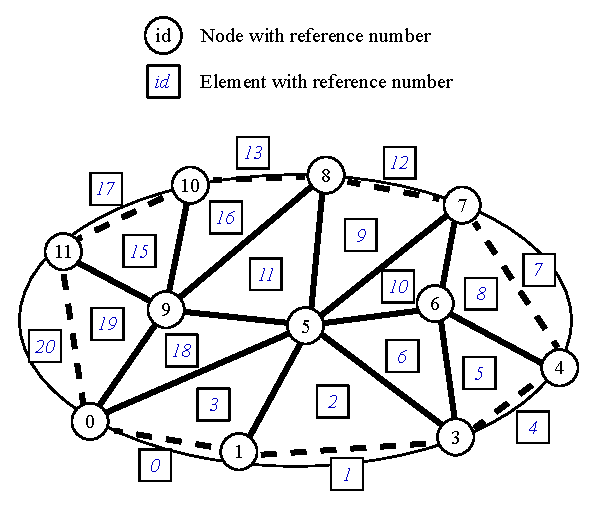
\includegraphics[width=\figwidth]{figures/FinleyMesh.eps}}
\caption{Subdivision of an Ellipse into triangles order 1 (\finleyelement{Tri3})}
\label{FINLEY FIG 0}
\end{figure}

\begin{figure}
\centerline{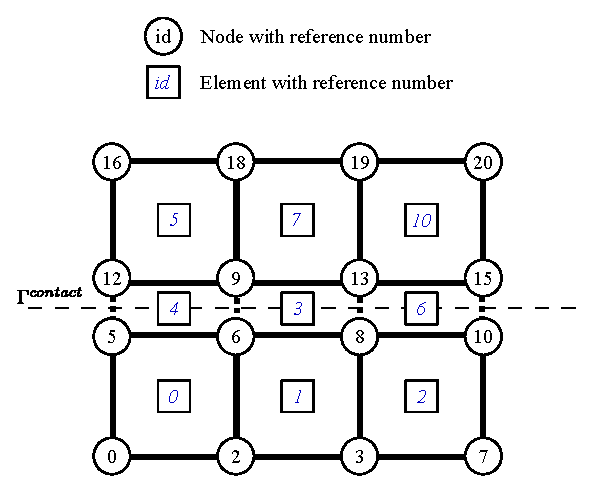
\includegraphics[width=\figwidth]{figures/FinleyContact.eps}}
\caption{Mesh around a contact region (\finleyelement{Rec4})}
\label{FINLEY FIG 01}
\end{figure}

\declaremodule{extension}{finley} \modulesynopsis{Solving linear, steady partial differential equations using
finite elements}

{\it finley} is a library of C functions solving linear, steady partial differential equations
\index{partial differential equations} (PDEs) or systems of PDEs using isoparametrical finite 
elements \index{FEM!isoparametrical}.
It supports unstructured, 1D, 2D and 3D meshes. The module \finley provides an access to the
library through the \LinearPDE class of \escript supporting its full functionality. {\it finley} 
is parallelized using the OpenMP \index{OpenMP} paradigm. 

\section{Formulation}

For a single PDE with a solution with a single component the linear PDE is defined in the
following form:
\begin{equation}\label{FINLEY.SINGLE.1}
\begin{array}{cl} &
\displaystyle{
\int\hackscore{\Omega} 
A\hackscore{jl} \cdot v\hackscore{,j}u\hackscore{,l}+ B\hackscore{j} \cdot v\hackscore{,j} u+ C\hackscore{l} \cdot v u\hackscore{,l}+D \cdot vu \; d\Omega }  \\
+ & \displaystyle{\int\hackscore{\Gamma} d \cdot vu \; d{\Gamma} } 
+  \displaystyle{\int\hackscore{\Gamma^{contact}} d^{contact} \cdot [v][u] \; d{\Gamma} } \\
= & \displaystyle{\int\hackscore{\Omega}  X\hackscore{j} \cdot v\hackscore{,j}+ Y \cdot v \; d\Omega }\\ 
+ & \displaystyle{\int\hackscore{\Gamma} y \cdot v \; d{\Gamma}}  + 
\displaystyle{\int\hackscore{\Gamma^{contact}} y^{contact}\cdot [v] \; d{\Gamma}} \\
\end{array}
\end{equation}

\section{Meshes}
To understand the usage of \finley one needs to have an understanding of how the finite element meshes
\index{FEM!mesh} are defined. \fig{FINLEY FIG 0} shows an example of the
subdivision of an ellipse into so called elements \index{FEM!elements} \index{element}. 
In this case, triangles have been used but other forms of subdivisions
can be constructed, e.g. into quadrilaterals or, in the three dimensional case, into tetrahedrons
and hexahedrons. The idea of the finite element method is to approximate the solution by a function
which is a polynomial of a certain order and is continuous across it boundary to neighbour elements.
In the example of \fig{FINLEY FIG 0} a linear polynomial is used on each triangle. As one can see, the triangulation
is quite a poor approximation of the ellipse. It can be improved by introducing a midpoint on each element edge then
positioning those nodes located on an edge expected to describe the boundary, onto the boundary.
In this case the triangle gets a curved edge which requires a parametrization of the triangle using a 
quadratic polynomial. For this case, the solution is also approximated by a piecewise quadratic polynomial
(which explains the name isoparametrical elements), see \Ref{Zienc,NumHand} for more details.   

The union of all elements defines the domain of the PDE.
Each element is defined by the nodes used to describe its shape. In \fig{FINLEY FIG 0} the element,
which has type \finleyelement{Tri3},
with element reference number $19$ \index{element!reference number} is defined by the nodes
with reference numbers $9$, $11$ and $0$ \index{node!reference number}. Notice that the order is counterclockwise. 
The coefficients of the PDE are evaluated at integration nodes with each individual element. 
For quadrilateral elements a Gauss quadrature scheme is used. In the case of triangular elements a 
modified form is applied. The boundary of the domain is also subdivided into elements. \index{element!face} In \fig{FINLEY FIG 0}
line elements with two nodes are used. The elements are also defined by their describing nodes, e.g.
the face element reference number $20$ which has type \finleyelement{Line2} is defined by the nodes
with the reference numbers $11$ and $0$. Again the order is crucial, if moving from the first
to second node the domain has to lie on the left hand side (in the case of a two dimension surface element
the domain has to lie on the left hand side when moving counterclockwise). If the gradient on the
surface of the domain is to be calculated rich face elements face to be used. Rich elements on a face
are identical to interior elements but with a modified order of nodes such that the 'first' face of the element aligns
with the surface of the domain. In \fig{FINLEY FIG 0}
elements of the type \finleyelement{Tri3Face} are used. 
The face element reference number $20$ as a rich face element is defined by the nodes
with reference numbers $11$, $0$ and $9$. Notice that the face element $20$ is identical to the
interior element $19$ except that, in this case, the order of the node is different to align the first
edge of the triangle (which is the edge starting with the first node) with the boundary of the domain.

Be aware that face elements and elements in the interior of the domain must match, i.e. a face element must be the face
of an interior element or, in case of a rich face element, it must be identical to an interior element.
If no face elements are specified
\finley implicitly assumes homogeneous natural boundary conditions \index{natural boundary conditions!homogeneous},
i.e. \var{d}=$0$ and \var{y}=$0$, on the entire boundary of the domain. For  
inhomogeneous natural boundary conditions \index{natural boundary conditions!inhomogeneous}, 
the boundary must be described by face elements. 

If discontinuities of the PDE solution are considered contact elements 
\index{element!contact}\index{contact conditions} are introduced to describe the contact region $\Gamma^{contact}$ 
even if $d^{contact}$ and $y^{contact}$ are zero. \fig{FINLEY FIG 01} shows a simple example of a mesh
of rectangular elements around a contact region $\Gamma^{contact}$ \index{element!contact}. 
The contact region is described by the
elements $4$, $3$ and $6$. Their element type is \finleyelement{Line2_Contact}. 
The nodes $9$, $12$, $6$, $5$ define contact element $4$, where the coordinates of nodes $12$ and $5$ and
nodes $4$ and $6$ are identical with the idea that nodes $12$ and $9$ are located above and 
nodes $5$ and $6$ below the contact region.  
Again, the order of the nodes within an element is crucial. There is also the option of using rich elements
if the gradient is to be calculated on the contact region. Similarly to the rich face elements 
these are constructed from two interior elements by reordering the nodes such that
the 'first' face of the element above and the 'first' face of the element below the 
contact regions line up.  The rich version of element 
$4$ is of type \finleyelement{Rec4Face_Contact} and is defined by the nodes $9$, $12$, $16$, $18$, $6$, $5$, $0$ and 
$2$.

\tab{FINLEY TAB 1} shows the interior element types and the corresponding element types to be used
on the face and contacts. \fig{FINLEY.FIG:1}, \fig{FINLEY.FIG:2} and \fig{FINLEY.FIG:4} show the ordering of
the nodes within an element.

\begin{table}
\begin{tablev}{l|llll}{textrm}{interior}{face}{rich face}{contact}{rich contact}
\linev{\finleyelement{Line2}}{\finleyelement{Point1}}{\finleyelement{Line2Face}}{\finleyelement{Point1_Contact}}{\finleyelement{Line2Face_Contact}}
\linev{\finleyelement{Line3}}{\finleyelement{Point1}}{\finleyelement{Line3Face}}{\finleyelement{Point1_Contact}}{\finleyelement{Line3Face_Contact}}
\linev{\finleyelement{Tri3}}{\finleyelement{Line2}}{\finleyelement{Tri3Face}}{\finleyelement{Line2_Contact}}{\finleyelement{Tri3Face_Contact}}
\linev{\finleyelement{Tri6}}{\finleyelement{Line3}}{\finleyelement{Tri6Face}}{\finleyelement{Line3_Contact}}{\finleyelement{Tri6Face_Contact}}
\linev{\finleyelement{Rec4}}{\finleyelement{Line2}}{\finleyelement{Rec4Face}}{\finleyelement{Line2_Contact}}{\finleyelement{Rec4Face_Contact}}
\linev{\finleyelement{Rec8}}{\finleyelement{Line3}}{\finleyelement{Rec8Face}}{\finleyelement{Line3_Contact}}{\finleyelement{Rec8Face_Contact}}
\linev{\finleyelement{Rec9}}{\finleyelement{Line3}}{\finleyelement{Rec9Face}}{\finleyelement{Line3_Contact}}{\finleyelement{Rec9Face_Contact}}
\linev{\finleyelement{Tet4}}{\finleyelement{Tri6}}{\finleyelement{Tet4Face}}{\finleyelement{Tri6_Contact}}{\finleyelement{Tet4Face_Contact}}
\linev{\finleyelement{Tet10}}{\finleyelement{Tri9}}{\finleyelement{Tet10Face}}{\finleyelement{Tri9_Contact}}{\finleyelement{Tet10Face_Contact}}
\linev{\finleyelement{Hex8}}{\finleyelement{Rec4}}{\finleyelement{Hex8Face}}{\finleyelement{Rec4_Contact}}{\finleyelement{Hex8Face_Contact}}
\linev{\finleyelement{Hex20}}{\finleyelement{Rec8}}{\finleyelement{Hex20Face}}{\finleyelement{Rec8_Contact}}{\finleyelement{Hex20Face_Contact}}
\end{tablev}
\caption{Finley elements and corresponding elements to be used on domain faces and contacts.
The rich types have to be used if the gradient of function is to be calculated on faces and contacts, respectively.}
\label{FINLEY TAB 1}
\end{table}

The native \finley file format is defined as follows.
Each node \var{i} has \var{dim} spatial coordinates \var{Node[i]}, a reference number
\var{Node_ref[i]}, a degree of freedom \var{Node_DOF[i]} and tag \var{Node_tag[i]}.
In most cases \var{Node_DOF[i]}=\var{Node_ref[i]} however, for periodic boundary conditions,
\var{Node_DOF[i]} is chosen differently, see example below. The tag can be used to mark nodes sharing
the same properties. Element \var{i} is defined by the \var{Element_numNodes} nodes \var{Element_Nodes[i]}
which is a list of node reference numbers. The order is crucial.
It has a reference number \var{Element_ref[i]} and a tag \var{Element_tag[i]}. The tag 
can be used to mark elements  sharing the same properties. For instance elements above 
a contact region are marked with $2$ and elements below a contact region are marked with $1$. 
\var{Element_Type} and \var{Element_Num} give the element type and the number of elements in the mesh.
Analogue notations are used for face and contact elements. The following Python script
prints the mesh definition in the \finley file format:
\begin{python}
print "%s\n"%mesh_name
# node coordinates:
print "%dD-nodes %d\n"%(dim,numNodes)
for i in range(numNodes): 
   print "%d %d %d"%(Node_ref[i],Node_DOF[i],Node_tag[i])
   for j in range(dim): print " %e"%Node[i][j]
   print "\n"
# interior elements
print "%s %d\n"%(Element_Type,Element_Num)
for i in range(Element_Num):
   print "%d %d"%(Element_ref[i],Element_tag[i])
   for j in range(Element_numNodes): print " %d"%Element_Nodes[i][j]
   print "\n"
# face elements
print "%s %d\n"%(FaceElement_Type,FaceElement_Num)
for i in range(FaceElement_Num):
   print "%d %d"%(FaceElement_ref[i],FaceElement_tag[i])
   for j in range(FaceElement_numNodes): print " %d"%FaceElement_Nodes[i][j]
   print "\n"
# contact elements
print "%s %d\n"%(ContactElement_Type,ContactElement_Num)
for i in range(ContactElement_Num):
   print "%d %d"%(ContactElement_ref[i],ContactElement_tag[i])
   for j in range(ContactElement_numNodes): print " %d"%ContactElement_Nodes[i][j]
   print "\n"
# point sources (not supported yet)
write("Point1 0",face_element_type,numFaceElements)
\end{python}

The following example of a mesh file defines the mesh shown in \fig{FINLEY FIG 01}:
\begin{verbatim}
Example 1
2D Nodes 16
0   0 0 0.   0.
2   2 0 0.33 0.
3   3 0 0.66 0.
7   4 0 1.   0.
5   5 0 0.   0.5
6   6 0 0.33 0.5
8   8 0 0.66 0.5
10 10 0 1.0  0.5
12 12 0 0.   0.5
9   9 0 0.33 0.5
13 13 0 0.66 0.5
15 15 0 1.0  0.5
16 16 0 0.   1.0
18 18 0 0.33 1.0
19 19 0 0.66 1.0
20 20 0 1.0  1.0
Rec4 6
 0 1  0  2  6  5
 1 1  2  3  8  6
 2 1  3  7 10  8
 5 2 12  9 18 16
 7 2 13 19 18  9
10 2 20 19 13 15
Line2 0
Line2_Contact 3
 4 0  9 12  6 5
 3 0 13  9  8 6
 6 0 15 13 10 8
Point1 0
\end{verbatim}
Notice that the order in which the nodes and elements are given is arbitrary.
In the case that rich contact elements are used the contact element section gets
 the form
\begin{verbatim}
Rec4Face_Contact 3
 4 0  9 12 16 18  6  5  0  2
 3 0 13  9 18 19  8  6  2  3
 6 0 15 13 19 20 10  8  3  7
\end{verbatim}
Periodic boundary condition \index{boundary conditions!periodic} can be introduced by altering \var{Node_DOF}.
It allows identification of nodes even if they have different physical locations. For instance, to
enforce periodic boundary conditions at the face $x_0=0$ and $x_0=1$ one identifies
the degrees of freedom for nodes $0$, $5$, $12$ and $16$ with the degrees of freedom for
$7$, $10$, $15$ and $20$, respectively. The node section of the \finley mesh gets now the form:  
\begin{verbatim}
2D Nodes 16
0   0 0 0.   0.
2   2 0 0.33 0.
3   3 0 0.66 0.
7   0 0 1.   0.
5   5 0 0.   0.5
6   6 0 0.33 0.5
8   8 0 0.66 0.5
10  5 0 1.0  0.5
12 12 0 0.   0.5
9   9 0 0.33 0.5
13 13 0 0.66 0.5
15 12 0 1.0  0.5
16 16 0 0.   1.0
18 18 0 0.33 1.0
19 19 0 0.66 1.0
20 16 0 1.0  1.0
\end{verbatim}


\include{finleyelements}

\subsection{Linear Solvers in \LinearPDE}
Currently \finley supports the linear solvers \PCG, \GMRES, \PRESTWENTY and \BiCGStab. 
For \GMRES the options \var{truncation} and \var{restart} of the \method{getSolution} can be
used to control the truncation and restart during iteration. Default values are
\var{truncation}=5 and \var{restart}=20.
The default solver is \BiCGStab  but if the symmetry flag is set \PCG is the default solver.
\finley supports the solver options \var{iter_max} which specifies the maximum number of iterations steps,
\var{verbose}=\True or \False and \var{preconditioner}=\constant{JACOBI} or \constant {ILU0}.
In some installations \finley supports the \Direct solver and the
solver options \var{reordering}=\constant{util.NO_REORDERING}, 
\constant{util.MINIMUM_FILL_IN} or \constant{util.NESTED_DISSECTION} (default is \constant{util.NO_REORDERING}),
\var{drop_tolerance} specifying the threshold for values to be dropped in the 
incomplete elimination process (default is 0.01) and \var{drop_storage} specifying the maximum increase 
in storage allowed in the 
incomplete elimination process (default is 1.20).

\subsection{Functions}
\begin{funcdesc}{Mesh}{fileName,integrationOrder=-1}
creates a \Domain object form the FEM mesh defined in 
file \var{fileName}. The file must be given the \finley file format.
If \var{integrationOrder} is positive, a numerical integration scheme
chosen which is accurate on each element up to a polynomial of
degree \var{integrationOrder} \index{integration order}. Otherwise
an appropriate integration order is chosen independently.
\end{funcdesc}

\begin{funcdesc}{Rectangle}{n0,n1,order=1,l0=1.,l1=1., integrationOrder=-1, \\
  periodic0=\False,periodic1=\False,useElementsOnFace=\False,optimize=\False}
Generates a \Domain object representing a two dimensional rectangle between
$(0,0)$ and $(l0,l1)$ with orthogonal edges. The rectangle is filled with
\var{n0} elements along the $x_0$-axis and
\var{n1} elements along the $x_1$-axis. 
For \var{order}=1 and \var{order}=2
\finleyelement{Rec4} and  
\finleyelement{Rec8} are used, respectively. 
In the case of \var{useElementsOnFace}=\False,
\finleyelement{Line2} and  
\finleyelement{Line3} are used to subdivide the edges of the rectangle, respectively. 
In the case of \var{useElementsOnFace}=\True (this option should be used if gradients
are calculated on domain faces),
\finleyelement{Rec4Face} and  
\finleyelement{Rec8Face} are used on the edges, respectively.  
If \var{integrationOrder} is positive, a numerical integration scheme
chosen which is accurate on each element up to a polynomial of
degree \var{integrationOrder} \index{integration order}. Otherwise
an appropriate integration order is chosen independently. If
\var{periodic0}=\True, periodic boundary conditions \index{periodic boundary conditions}
along the $x_0$-directions are enforced. That means when for any solution of a PDE solved by \finley
the value on the line $x_0=0$ will be identical to the values on $x_0=\var{l0}$.
Correspondingly,
\var{periodic1}=\False sets periodic boundary conditions
in $x_1$-direction.
If \var{optimize}=\True mesh node relabeling will be attempted to reduce the computation and also ParMETIS will be used to improve the mesh partition if running on multiple CPUs with MPI.
\end{funcdesc}

\begin{funcdesc}{Brick}{n0,n1,n2,order=1,l0=1.,l1=1.,l2=1., integrationOrder=-1, \\
  periodic0=\False,periodic1=\False,periodic2=\False,useElementsOnFace=\False,optimize=\False}
Generates a \Domain object representing a three dimensional brick between
$(0,0,0)$ and $(l0,l1,l2)$ with orthogonal faces. The brick is filled with
\var{n0} elements along the $x_0$-axis, 
\var{n1} elements along the $x_1$-axis and 
\var{n2} elements along the $x_2$-axis. 
For \var{order}=1 and \var{order}=2
\finleyelement{Hex8} and  
\finleyelement{Hex20} are used, respectively. 
In the case of \var{useElementsOnFace}=\False,
\finleyelement{Rec4} and  
\finleyelement{Rec8} are used to subdivide the faces of the brick, respectively. 
In the case of \var{useElementsOnFace}=\True (this option should be used if gradients
are calculated on domain faces),
\finleyelement{Hex8Face} and  
\finleyelement{Hex20Face} are used on the brick faces, respectively.  
If \var{integrationOrder} is positive, a numerical integration scheme
chosen which is accurate on each element up to a polynomial of
degree \var{integrationOrder} \index{integration order}. Otherwise
an appropriate integration order is chosen independently. If
\var{periodic0}=\True, periodic boundary conditions \index{periodic boundary conditions}
along the $x_0$-directions are enforced. That means when for any solution of a PDE solved by \finley
the value on the plane $x_0=0$ will be identical to the values on $x_0=\var{l0}$. Correspondingly,
\var{periodic1}=\False and \var{periodic2}=\False sets periodic boundary conditions
in $x_1$-direction and $x_2$-direction, respectively.
If \var{optimize}=\True mesh node relabeling will be attempted to reduce the computation and also ParMETIS will be used to improve the mesh partition if running on multiple CPUs with MPI.
\end{funcdesc}

\begin{funcdesc}{GlueFaces}{meshList,safetyFactor=0.2,tolerance=1.e-13}
Generates a new \Domain object from the list \var{meshList} of \finley meshes.
Nodes in face elements whose difference of coordinates is less then \var{tolerance} times the 
diameter of the domain are merged. The corresponding face elements are removed from the mesh.  

TODO: explain \var{safetyFactor} and show an example.
\end{funcdesc}

\begin{funcdesc}{JoinFaces}{meshList,safetyFactor=0.2,tolerance=1.e-13}
Generates a new \Domain object from the list \var{meshList} of \finley meshes.
Face elements whose nodes coordinates have difference is less then \var{tolerance} times the 
diameter of the domain are combined to form a contact element \index{element!contact} 
The corresponding face elements are removed from the mesh.  

TODO: explain \var{safetyFactor} and show an example.
\end{funcdesc}


\input{troubleshooting}
\makemodindex

\printindex
%% $Id$
\documentclass{manual}

% grab the handy definitions and \usepackage statements etc
\input{guide_defs}

% title, author, etc stuff
\title{ESyS Users Guide}

\author{Lutz Gross (Editor)}
\authoraddress{
Earth Systems Science Computational Centre (ESSCC) \\
The University of Queensland \\
Australia \\
Email: \email{esys@access.edu.au}
}                                                                                         
\date{\today}      
\release{$Id$}
\setreleaseinfo{} 
\setshortversion{}

\makeindex

% the actual start of the document
\begin{document}

\maketitle

\input{copyrights}

\begin{abstract}
This document is a guide of how to use the \ESyS software and
associated tools.
\end{abstract}

\tableofcontents

\input{introduction}
\input{firststep}
\input{diffusion}
% \input{wavepropagation}

\input{escript}
\input{linearPDE}
%\input{bruce}
\input{finley}

\input{troubleshooting}
\makemodindex

\printindex
%\input{guide.ind}

\bibliographystyle{plain}
\bibliography{esys}

\end{document}


\bibliographystyle{plain}
\bibliography{esys}

\end{document}


\bibliographystyle{plain}
\bibliography{esys}

\end{document}


\bibliographystyle{plain}
\bibliography{esys}

\end{document}
